\graphicspath{{capitulos/Capitulo5-Resultados-experimentales/recursos/}}

\section{Resultados experimentales} \label{capitulo:5}
%En este capítulo se detallan los casos de prueba empleados para la parte de experimentación realizada para este TFM. La metaheurística de la \fasedos{} del sistema (definida en la \autoref{sec:3:metaheurística}) consta de un conjunto de parámetros, enumerados en esta sección, que afectan al rendimiento de esta. Se ha analizado para cada caso, los valores de cada parámetro que mejores resultados ofrecen.

En este capítulo se detallan los procesos realizados para la parte de experimentación realizada en este TFM. En primer lugar, se definen los casos de prueba empleados, posteriormente se detalla el proceso de ajuste de los parámetros, presente en toda metaheurística y que nos permite fijar los parámetros del VNS empleado en la \fasedos{} del sistema (definida en la \autoref{sec:3:metaheurística}) a aquellos valores que ofrecen mejores resultados. A continuación, se ha hecho una comparación de rendimiento de la metaheurística implementada frente a la ya mencionada metaheurística \sa{}, y se hace un análisis en profundidad de algunos de los casos.

Las ejecuciones presentadas a lo largo de este capítulo han sido realizadas en un ordenador con las características recopiladas en la \autoref{table:5:caracteristicas-pc}.

\begin{table}[h]
	\centering
	\caption{Características del ordenador empleado para la experimentación}
	\begin{tabular}{lcc}
		\hline
		Procesador   & Intel Core i7 &  \\
		Memoria      &     16GB      &  \\
		Version Java &    JDK 8.1    &  \\ \hline
		             &               &
	\end{tabular}
\label{table:5:caracteristicas-pc}
\end{table}

\subsection{Definición de los casos de prueba}
\label{sec:5:def-casos}

Para este capítulo se han utilizado un conjunto de casos (instancias) de prueba reales que fueron proporcionados por CRIDA. Inicialmente, CRIDA facilitó la información en los formatos de ficheros propuestos (véase \autoref{sec:4:req-io} y \autoref{Anexo:formato-planificacion-inicial}) que fue adaptada para conformar los 8 casos de prueba distintos que se han empleado y definiremos a continuación. Una descripción de los casos de prueba más detallada se encuentra incluida en el \autoref{Anexo:tabla-casos}, junto con una tabla resumen de los casos que permite ver de forma más detallada y clara las características de cada uno de ellos.

Los casos de prueba se numeran del 1 al 9, a excepción del Caso 2, para el que \gls{CRIDA} no facilitó todos los datos y se decidió mantener el número identificativo de los demás casos por si en un futuro se completase con la información restante.

Los casos prueban el sistema empleando distintas Unidades de Control: Madrid, Barcelona y Palma de Mallorca; variando en cada uno el problema a resolver: modificación de la sectorización, baja (y alta en algún caso) de un controlador, o incluso ambos.

Los casos 5 y 7 resuelven los dos problemas a la vez: el cambio de sectorización y baja+alta de un controlador, por lo que son las instancias del problema más costosas de todas, y como veremos, son las que peores resultados alcanzan.

Por otro lado, cabe destacar que el Caso 5, 8 y 9 requiere del uso de un controlador imaginario (para la inicialización realizada en la \faseuno{}), y el Caso 7 requiere de cuatro (3 para un nuevo sector, 1 para la baja del controlador), mientras que el resto no necesitan ningún controlador imaginario para la inicialización. En los citados casos, el objetivo \ref{O1} tomará la máxima importancia hasta que alcance su valor máximo de 1, mientras que en los demás, el valor inicial de este ya es de uno, por lo que la búsqueda se dedicará exclusivamente al resto de los objetivos.

% % % % % % % % % % % % % % % % % % % % % % %
% % % % % % % % % % % % % % % % % % % % % % %
% % %		ESTE DOCUMENTO ES UN		% % %
% % %       COPIA-PEGA ADAPTADO		    % % %
% % %       DEL ORIGINAL ANEXO D		% % %
% % % % % % % % % % % % % % % % % % % % % % %
% % % % % % % % % % % % % % % % % % % % % % %


A continuación, detallamos los casos de prueba empleados en el TFM. Recuérdese que ésta información está resumida para una consulta más sencilla en una tabla adjunta en el \autoref{Anexo:tabla-casos}. En la \autoref{sec:5:comparacion-metaheuristicas} se describen los resultados de cada caso en cada una de las fases.

Las abreviaturas que representan los tipos de turno son las siguientes:

\begin{enumerate}[align=left]
	\item[M] Mañana
	\item[T] Tarde 
	\item[ML] Mañana Largo
	\item[MC] Mañana Corto
	\item[TL] Tarde Largo
	\item[TC] Tarde Corto
	\item[N] Noche
\end{enumerate}

\subsubsection{Caso 1}

\textbf{Unidad de Control}: Barcelona

\textbf{Turno}: MC, 7:30 -- 15:00

\textbf{Núcleos}: Ruta Este, Ruta Oeste

\textbf{Situación inicial}:
\begin{itemize}[label={}]
		
	\item \textbf{Recursos}: \\
	7 PTD Barcelona Ruta Este \\
	17 PTD Barcelona Ruta Oeste
	
	
	\item \textbf{Sectorización}: véase la \autoref{table:5:caso1-inicial}
	
	\item Planificación inicial: véase la \autoref{fig:caso1-fase0}
	
	\begin{figure}[h]
		\centering
		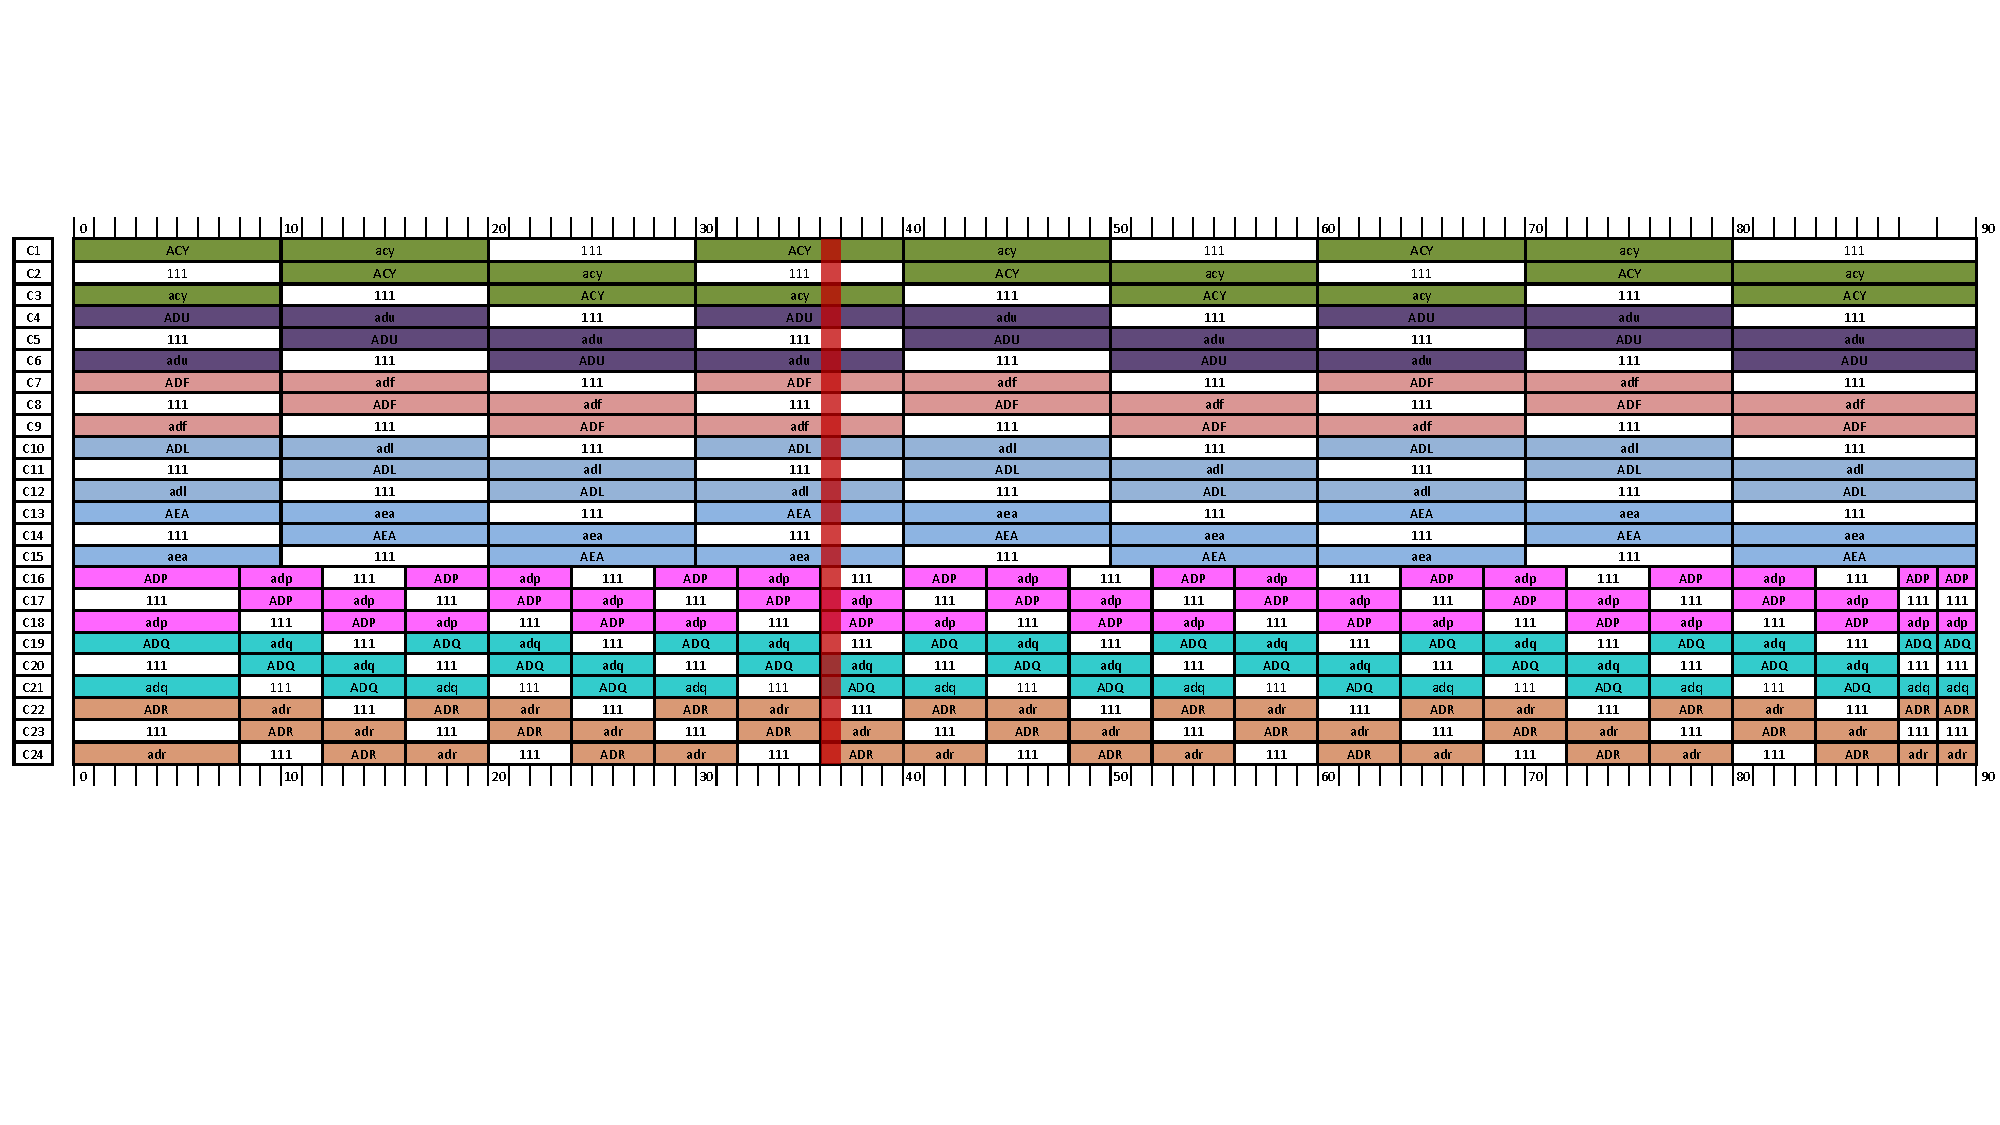
\includegraphics[width=\linewidth]{caso1/caso1-fase0}
		\caption{Planificación inicial del Caso 1}
		\label{fig:caso1-fase0}
	\end{figure}
	
	\begin{table}[h]
		\centering
		\caption{Sectorización inicial del Caso 1}
		\begin{tabular}{ccc}
			\hline
			\textbf{Núcleo}      & \textbf{Configuración} & \textbf{Intervalo}   \\ \hline
			\multicolumn{1}{l}{} & \multicolumn{1}{l}{}   & \multicolumn{1}{l}{} \\
			Barcelona Ruta Este  & 3D                     & 7:30:00--15:00:00    \\
			\multicolumn{1}{l}{} & \multicolumn{1}{l}{}   & \multicolumn{1}{l}{} \\
			Barcelona Ruta Oeste & 5A                     & 10:30:00--15:00:00   \\ \hline
		\end{tabular}
		\label{table:5:caso1-inicial}
	\end{table}
	
\end{itemize}

\textbf{Momento del Cambio}: 10:30:00

\textbf{Tipo incidencia}: Modificación de sectorizaciones

\textbf{Descripción}: Pasamos de una 3D a una 5A, lo que implica el cierre de un sector y la apertura de otros dos. Además se abre un sector adicional en el núcleo \textit{Barcelona Ruta Oeste}. La nueva sectorización es la de la \autoref{table:5:caso1-modif}. Se necesitan 3 controladores imaginarios para inicializar este caso.

\begin{table}[h]
	\centering
	\caption{Sectorización modificada del Caso 1}
	\begin{tabular}{ccc}
		\hline
		\textbf{Núcleo}                                           & \textbf{Configuración} & \textbf{Intervalo}   \\ \hline
		\multicolumn{1}{l}{}                                      & \multicolumn{1}{l}{}   & \multicolumn{1}{l}{} \\
		\multicolumn{1}{c|}{\multirow{2}{*}{Barcelona Ruta Este}} & 3D                     & 7:30:00--15:00:00    \\
		\multicolumn{1}{c|}{}                                     & 5A                     & 7:30:00--10:30:00    \\
		\multicolumn{1}{l}{}                                      & \multicolumn{1}{l}{}   & \multicolumn{1}{l}{} \\
		Barcelona Ruta Oeste                                      & 6C                     & 10:30:00--15:00:00   \\ \hline
	\end{tabular}
	\label{table:5:caso1-modif}
\end{table}


\subsubsection[Caso 3]{Caso 3\footnote{Nótese que se ha saltado el Caso 2. Esto se debe a que el correspondiente Caso 2 enviado por \gls{CRIDA} tenía una falta de datos que impedía su uso. Se ha decidido mantener la misma nomenclatura para una concordancia total con el código entregado.}}

\textbf{Unidad de Control}: Barcelona

\textbf{Turno}: MC, 7:30 -- 15:00

\textbf{Núcleos}: Ruta Este, Ruta Oeste

\textbf{Situación inicial}:
\begin{itemize}[label={}]
	
	\item \textbf{Recursos}: \\
	7 PTD Barcelona Ruta Este \\
	17 PTD Barcelona Ruta Oeste
	
	
	\item \textbf{Sectorización}: véase la \autoref{table:5:caso3-inicial}
	
	\item Planificación inicial: véase la \autoref{fig:5:caso3-fase0}
	
	\begin{figure}[!h]
		\centering
		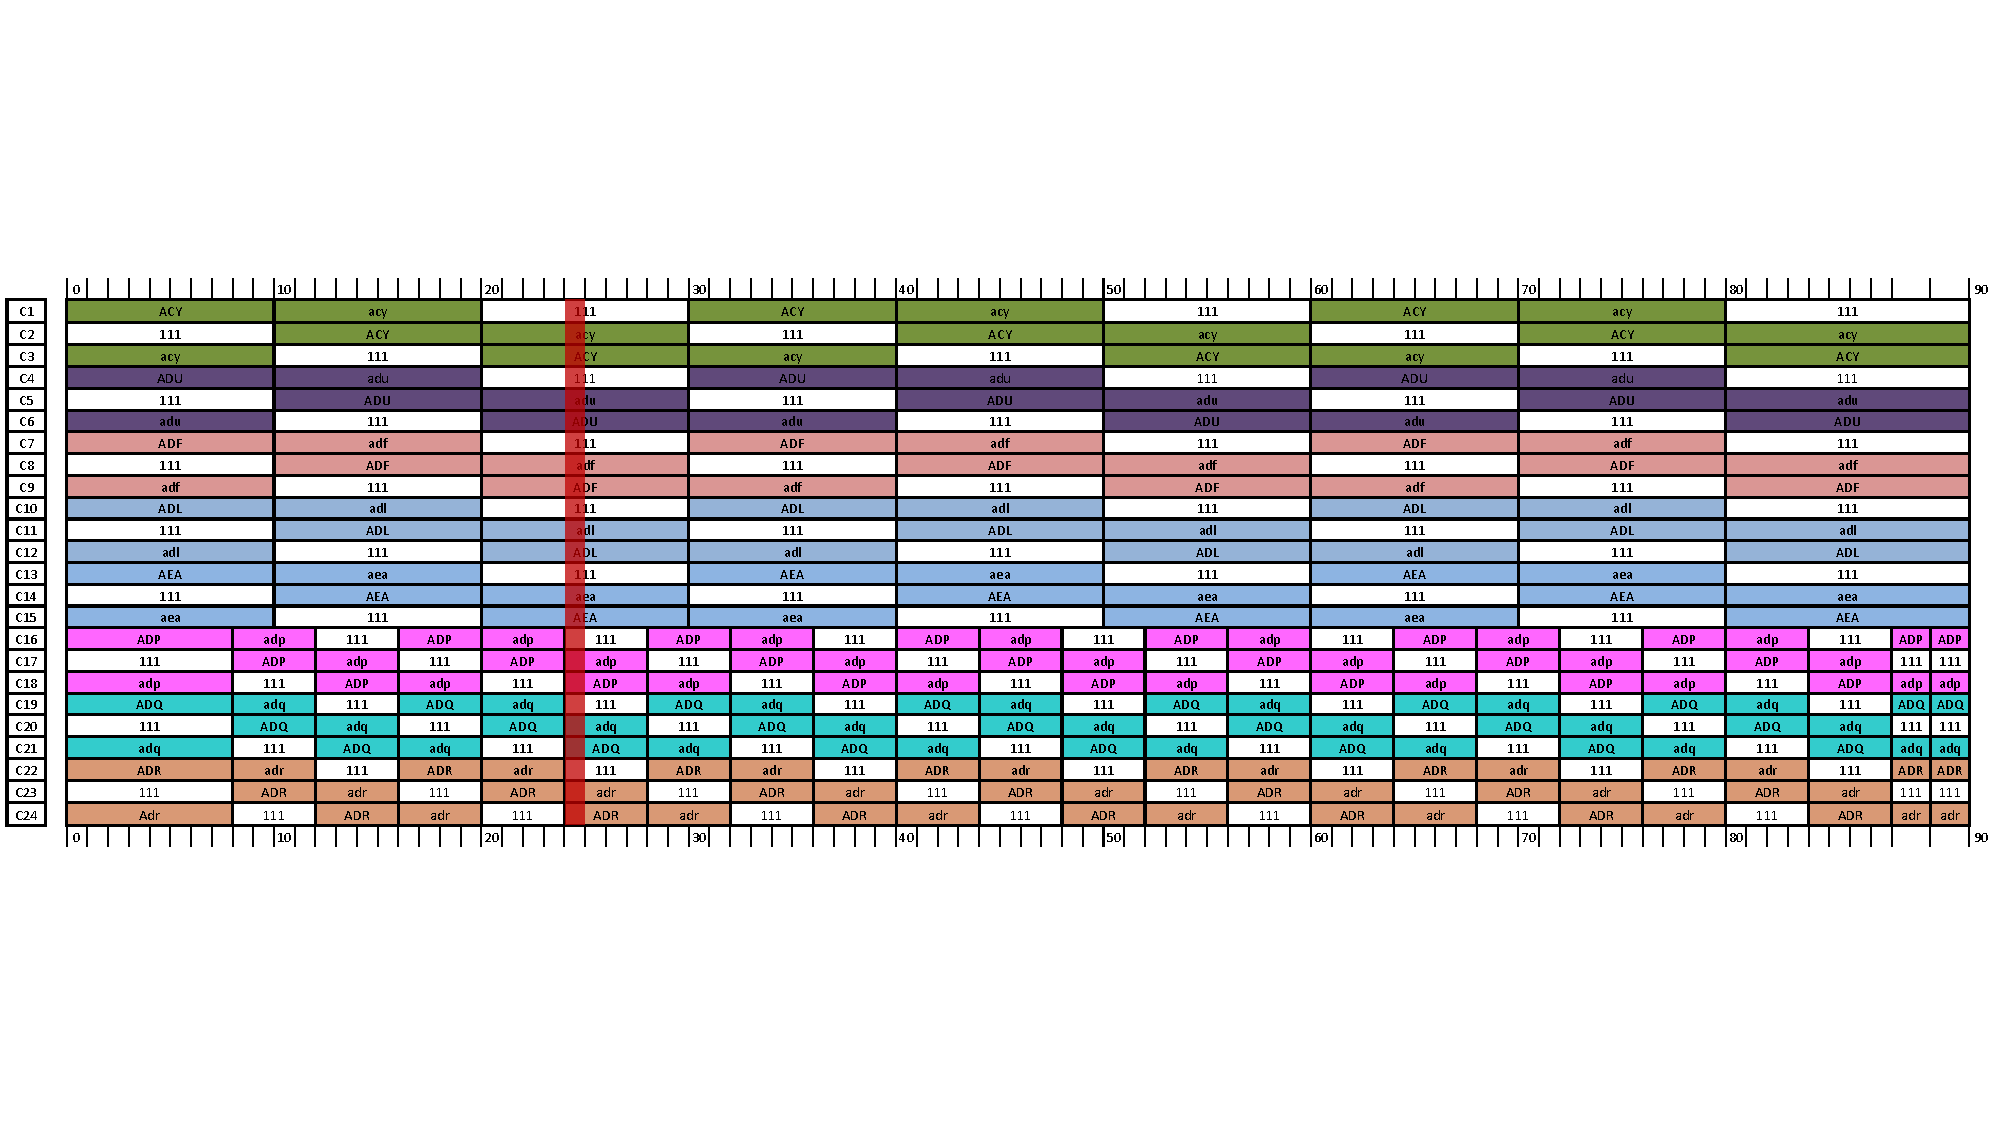
\includegraphics[width=\linewidth]{caso3/caso3-fase0}
		\caption{Planificación inicial del Caso 3}
		\label{fig:5:caso3-fase0}
	\end{figure}

	\begin{table}[h]
		\centering
		\caption{Sectorización inicial del Caso 1}
		\begin{tabular}{ccc}
			\hline
			\textbf{Núcleo}      & \textbf{Configuración} & \textbf{Intervalo}   \\ \hline
			\multicolumn{1}{l}{} & \multicolumn{1}{l}{}   & \multicolumn{1}{l}{} \\
			Barcelona Ruta Este  & 3D                     & 7:30:00--15:00:00    \\
			\multicolumn{1}{l}{} & \multicolumn{1}{l}{}   & \multicolumn{1}{l}{} \\
			Barcelona Ruta Oeste & 5A                     & 10:30:00--15:00:00   \\ \hline
		\end{tabular}
		\label{table:5:caso3-inicial}
	\end{table}
	
\end{itemize}

\textbf{Momento del Cambio}: 9:30:00 (slot 24)

\textbf{Tipo incidencia}: Baja de un controlador

\textbf{Descripción}: Se produce una baja del controlador C23 a las 9:30 (slot 24). No se producen altas. Se necesita 1 controlador imaginario para inicializar este caso.


\subsubsection{Caso 4}

\textbf{Unidad de Control}: Madrid

\textbf{Turno}: TC, 15:00 -- 22:30

\textbf{Núcleo}: Madrid TMA

\textbf{Situación inicial}:
\begin{itemize}[label={}]
	
	\item \textbf{Recursos}: \\
	19 PTD Madrid TMA
	
	
	\item \textbf{Sectorización}: véase la \autoref{table:5:caso4-inicial}
	
	\item Planificación inicial: véase la \autoref{fig:5:caso4-fase0}
	
	\begin{figure}[!h]
		\centering
		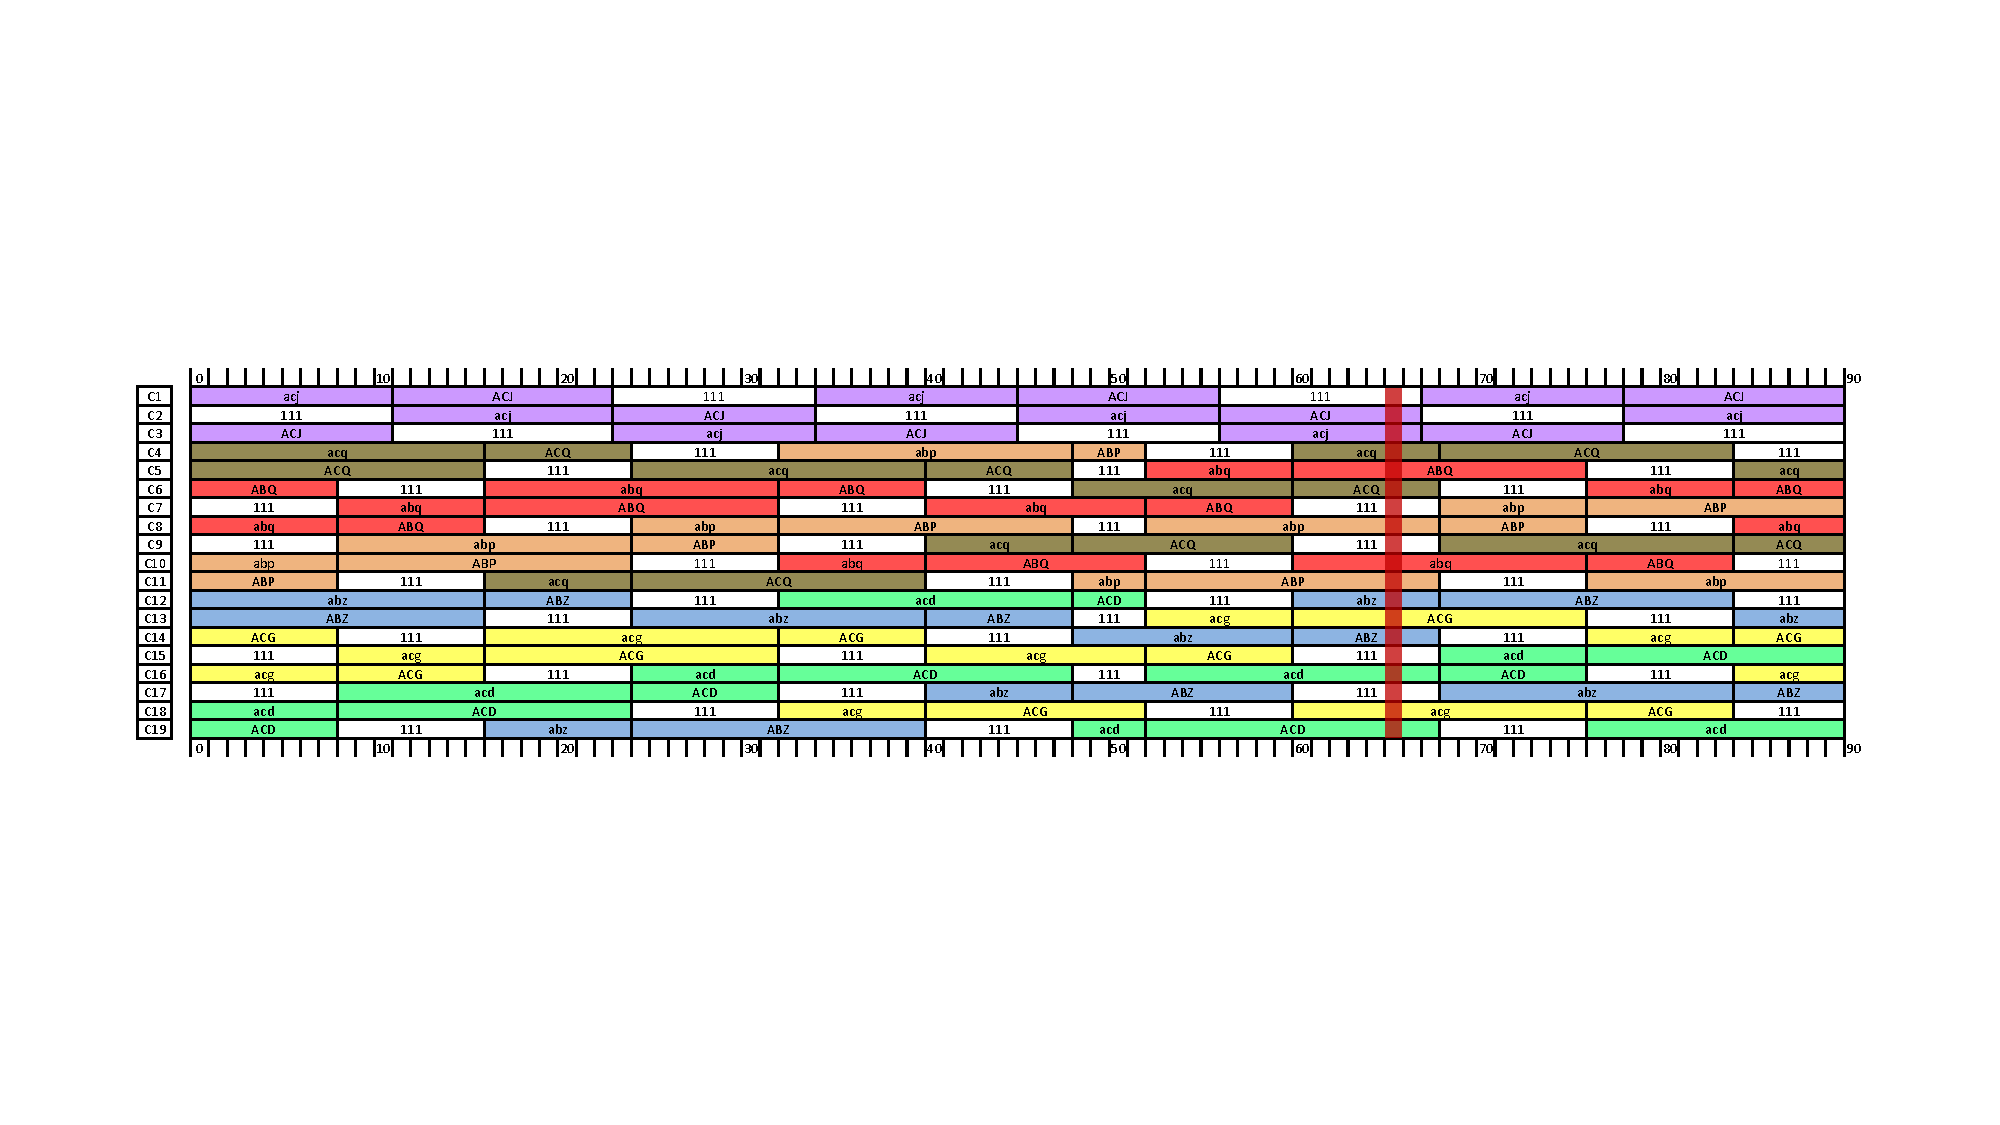
\includegraphics[width=\linewidth]{caso4/caso4-fase0}
		\caption{Planificación inicial del Caso 4}
		\label{fig:5:caso4-fase0}
	\end{figure}

	\begin{table}[h]
		\centering
		\caption{Sectorización inicial del Caso 4}
		\label{table:5:caso4-inicial}
		\begin{tabular}{ccc}
			\hline
			\textbf{Núcleo} & \textbf{Configuración} & \textbf{Intervalo} \\ \hline
			Madrid TMA             & 7BN                                      & 15:00:00 -- 22:30:00                \\ \hline
		\end{tabular}
	\end{table}
\end{itemize}

\textbf{Momento del Cambio}: 20:40:00  (slot 65)

\textbf{Tipo incidencia}: Modificación de sectorizaciones.

\textbf{Descripción}: Se divide la sectorización en cuatro intervalos sucesivos: 7 sectores durante 5:40 horas, 4 durante los 40 minutos siguientes y 3 durante los 10 últimos minutos, como se muestra en la \autoref{table:D:caso4-modif}. No se emplean controladores imaginarios.

\begin{table}[h]
	\centering
	\caption{Sectorización modificada del Caso 4.}
	\label{table:D:caso4-modif}
	\begin{tabular}{lcl}
		\hline
		\multicolumn{1}{c}{\textbf{Núcleo}}              & \textbf{Configuración} & \multicolumn{1}{c}{\textbf{Intervalo}} \\ \hline
		& \multicolumn{1}{l}{}   &                                        \\
		\multicolumn{1}{l|}{\multirow{4}{*}{Madrid TMA}} & 7BN                    & 15:00 -- 20:40                         \\
		\multicolumn{1}{l|}{}                            & 5DN                    & 20:40 -- 21:00                         \\
		\multicolumn{1}{l|}{}                            & 4CN                    & 21:00 -- 21:40                         \\
		\multicolumn{1}{l|}{}                            & 3AN                    & 21:40 -- 22:30                         \\
		\multicolumn{1}{c}{}                             &                        & \multicolumn{1}{c}{}                   \\ \hline
	\end{tabular}
\end{table}

\subsubsection{Caso 5}

\textbf{Unidad de Control}: Madrid

\textbf{Turno}: TC, 15:00 -- 22:30

\textbf{Núcleo}: Madrid TMA

\textbf{Situación inicial}:
\begin{itemize}[label={}]
	
	\item \textbf{Recursos}: \\
	7 PTD Barcelona Ruta Este \\
	17 PTD Barcelona Ruta Oeste
	
	
	\item \textbf{Sectorización}: véase la \autoref{table:5:caso4-inicial}
	
	\item Planificación inicial: véase la \autoref{fig:caso5-fase0}

	\begin{figure}[!h]
		\centering
		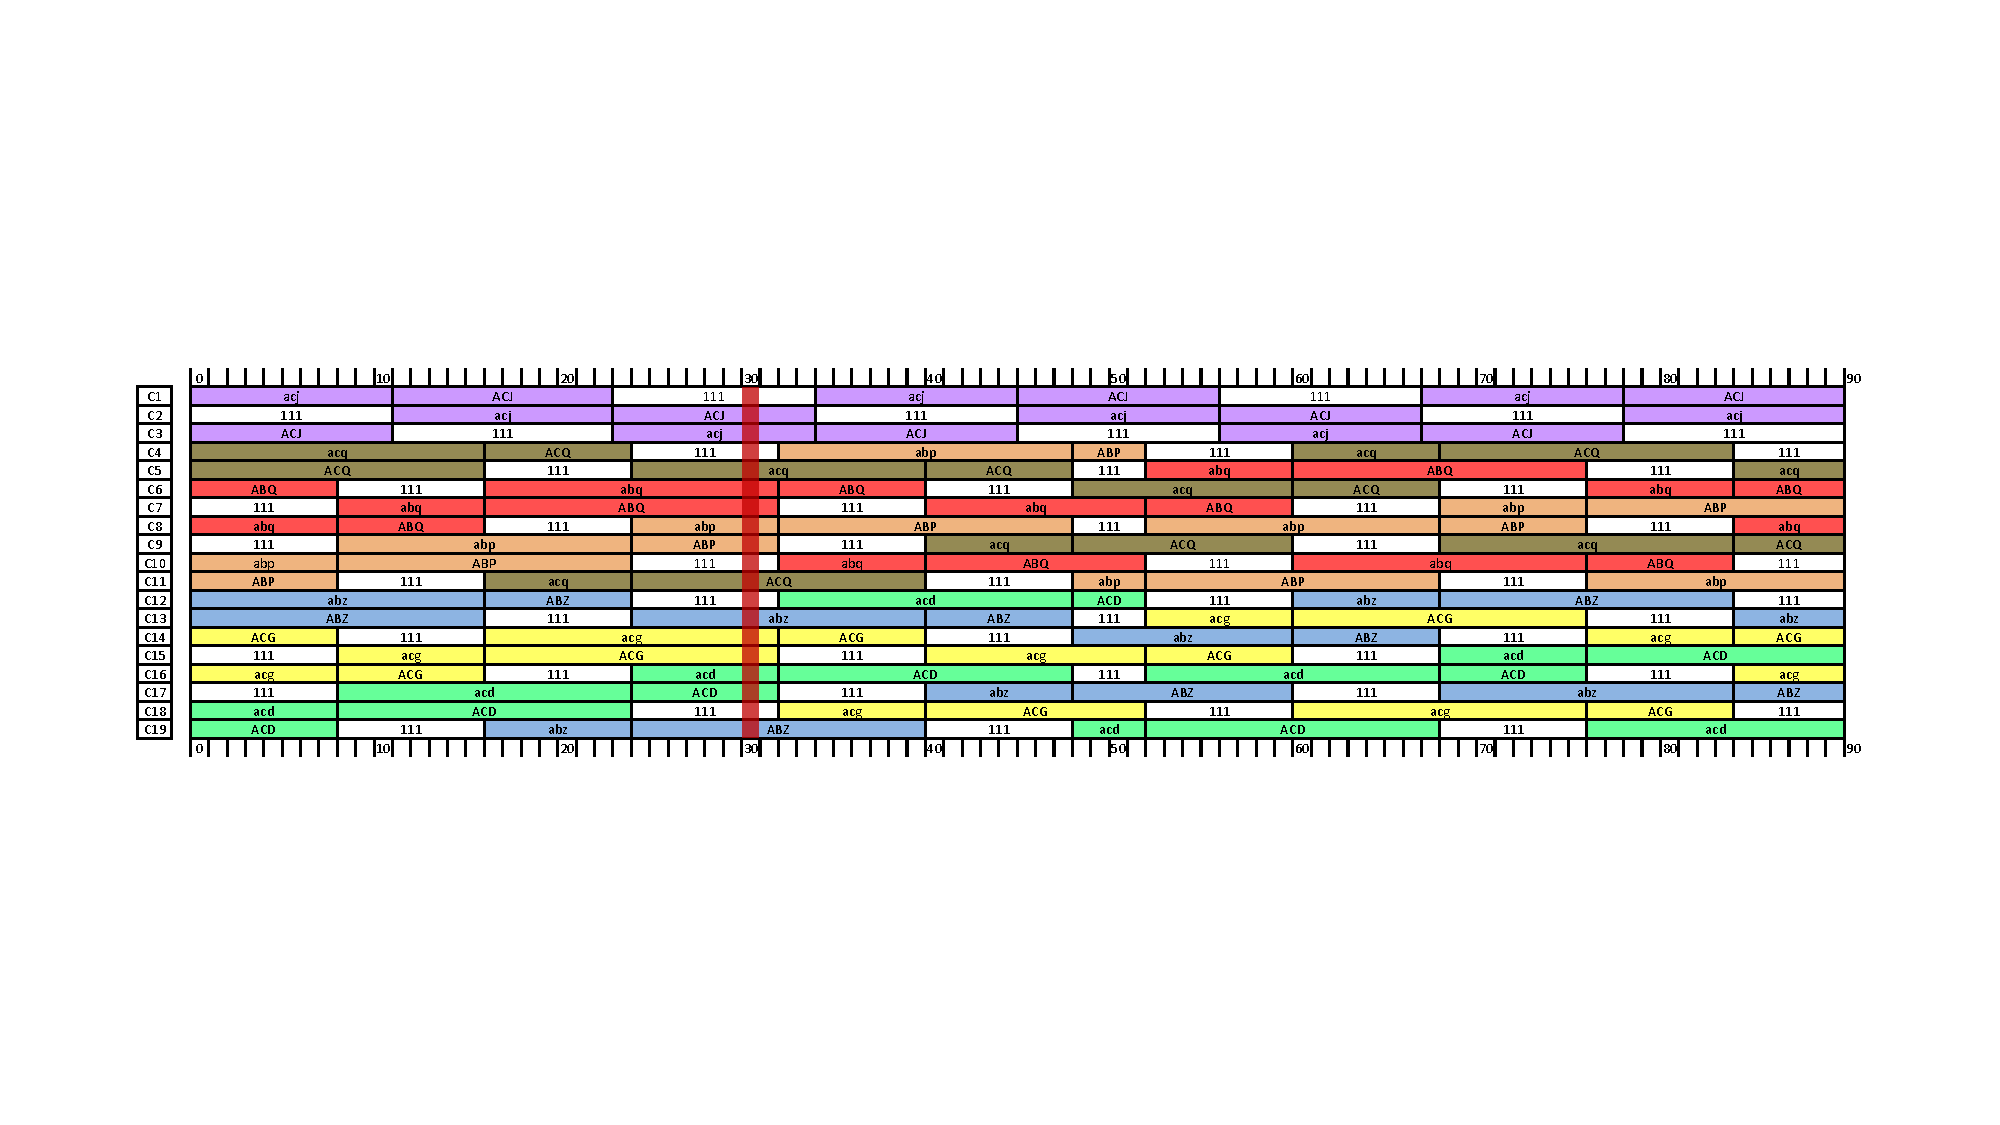
\includegraphics[width=\linewidth]{caso5/caso5-fase0}
		\caption{Planificación inicial del Caso 5}
		\label{fig:5:caso5-fase0}
	\end{figure}

\end{itemize}

\textbf{Momento del Cambio}: 17:30:00 (slot 30)

\textbf{Tipo incidencia}: Modificación de sectorizaciones, baja de un controlador, alta de un controlador.

\textbf{Descripción}: Además de la incidencia del Caso 4 (\autoref{table:D:caso4-modif}), también se produce la baja del controlador C8 a las 17:30 (slot 30) y el alta de un nuevo controlador a las 20:20 (slot 64). Se requiere del uso de un controlador imaginario.

\subsubsection{Caso 6}

\textbf{Unidad de Control}: Madrid

\textbf{Turno}: TC, 15:00 -- 22:30

\textbf{Núcleo}: Madrid TMA

\textbf{Situación inicial}:
\begin{itemize}[label={}]
	
	\item \textbf{Recursos}: \\
	7 PTD Barcelona Ruta Este \\
	17 PTD Barcelona Ruta Oeste
	
	
	\item \textbf{Sectorización}: véase la \autoref{table:5:caso4-inicial}
	
	\item Planificación inicial: véase la \autoref{fig:5:caso6-fase0}
	
	\begin{figure}[!h]
		\centering
		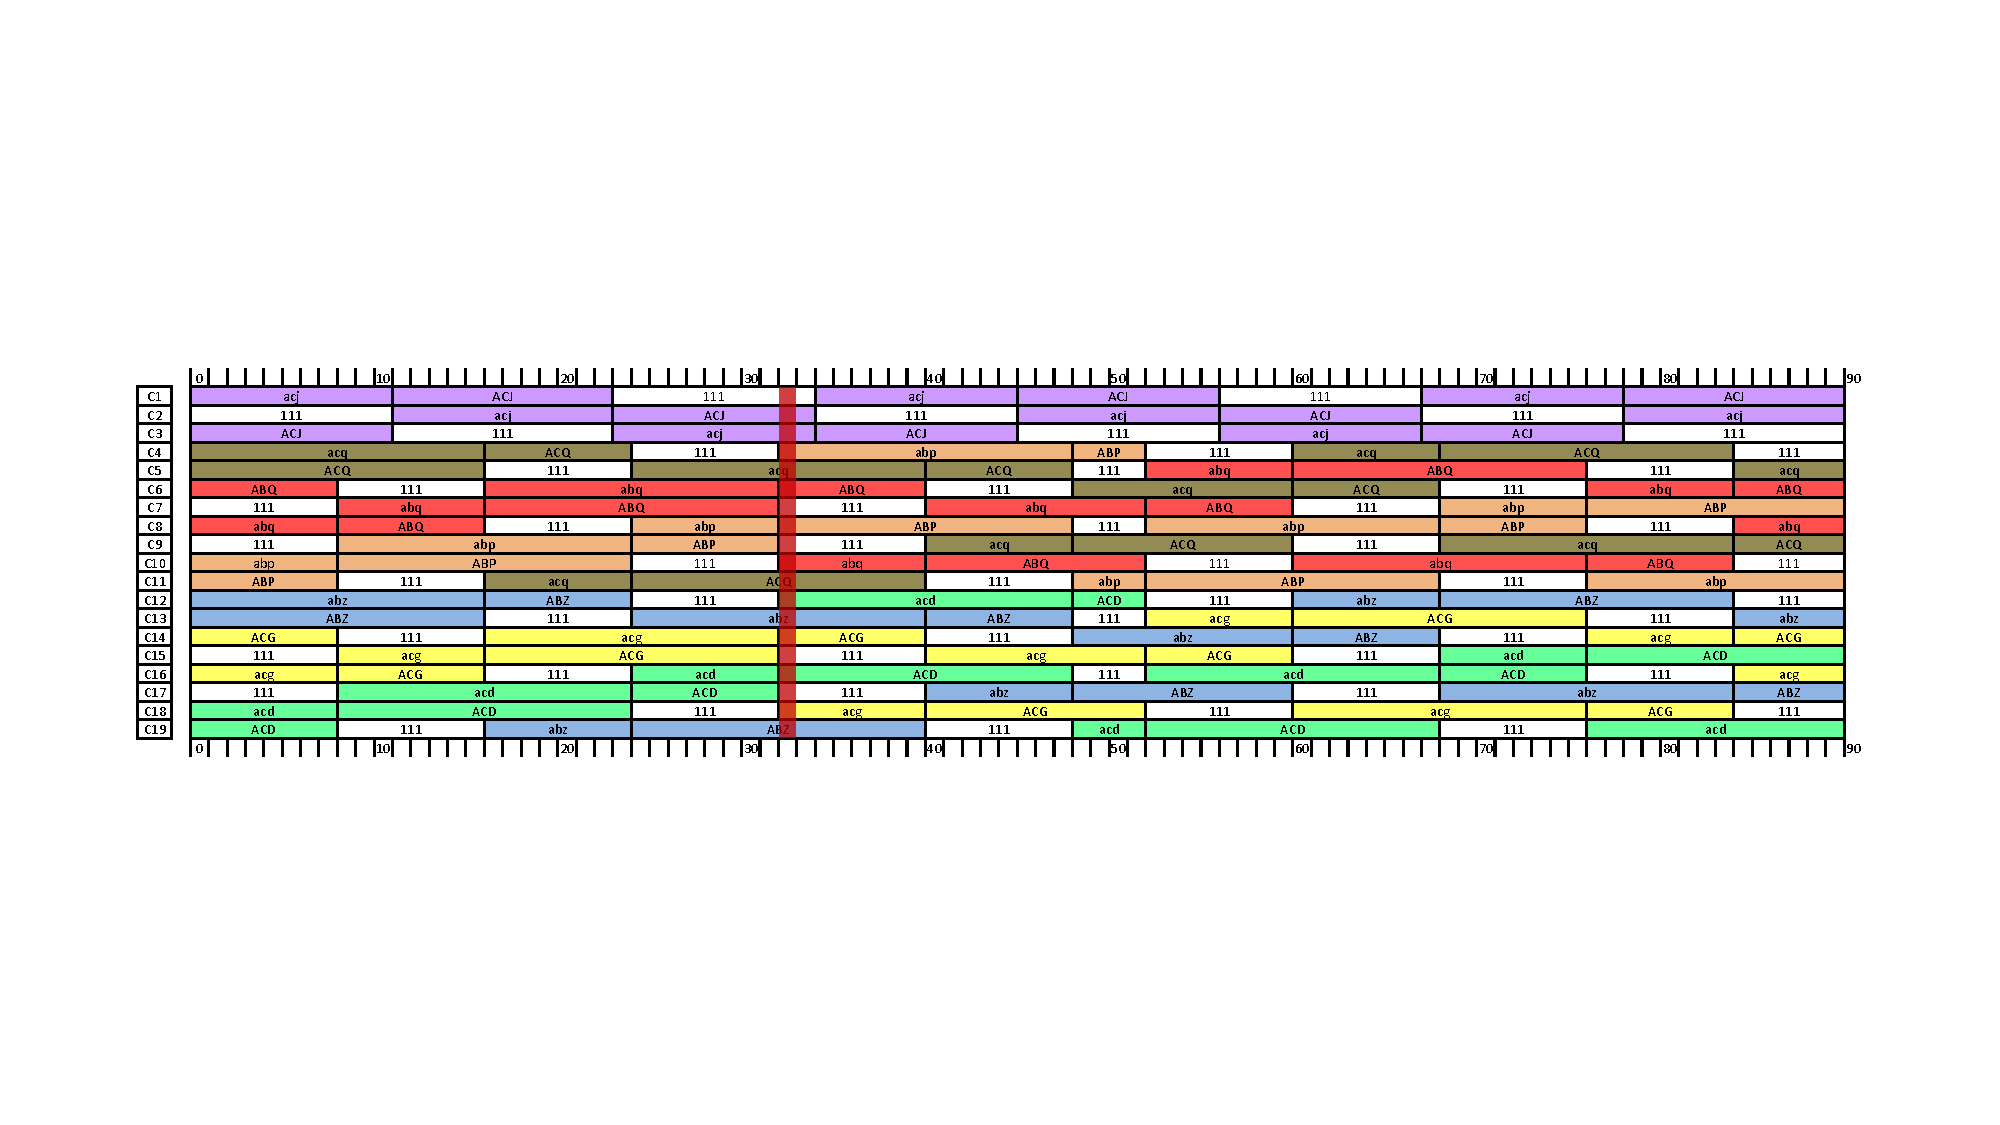
\includegraphics[width=\linewidth]{caso6/caso6-fase0}
		\caption{Planificación inicial del Caso 6}
		\label{fig:5:caso6-fase0}
	\end{figure}
	
	
\end{itemize}

\textbf{Momento del Cambio}: 17:40:00 (slot 32)

\textbf{Tipo incidencia}: Modificación de sectorizaciones.

\textbf{Descripción}: Se divide la sectorización en cuatro intervalos sucesivos: 7 sectores durante 5:40 horas, 4 durante los 40 minutos siguientes y 3 durante los 10 últimos minutos, como se muestra en la \autoref{table:D:caso6-modif}. No es necesario el uso de ningún controlador imaginario.

% Please add the following required packages to your document preamble:
% \usepackage{multirow}
\begin{table}[h]
	\centering
	\caption{Sectorización modificada del Caso 6.}
	\label{table:D:caso6-modif}
	\begin{tabular}{ccc}
		\hline
		\multicolumn{1}{c}{\textbf{Núcleo}}              & \multicolumn{1}{c}{\textbf{Configuración}} & \multicolumn{1}{c}{\textbf{Intervalo}} \\ \hline
		&                                            &                                        \\
		\multicolumn{1}{l|}{\multirow{5}{*}{Madrid TMA}} & 7BN                                        & 15:00 -- 17:40                         \\
		\multicolumn{1}{l|}{}                            & 8DN                                        & 17:40 -- 20:40                         \\
		\multicolumn{1}{l|}{}                            & 7BN                                        & 20:40 -- 21:00                         \\
		\multicolumn{1}{l|}{}                            & 4BN                                        & 21:00 -- 21:20                         \\
		\multicolumn{1}{l|}{}                            & 3AN                                        & 21:20 -- 22:30                         \\
		\multicolumn{1}{c}{}                             &                                            &                                        \\ \hline
	\end{tabular}
\end{table}


\subsubsection{Caso 7}

\textbf{Unidad de Control}: Barcelona

\textbf{Turno}: TC, 15:00 -- 21:35


\textbf{Núcleos}: Ruta Este, Ruta Oeste

\textbf{Situación inicial}:
\begin{itemize}[label={}]
	
	\item \textbf{Recursos}: \\
	11 PTD Barcelona Ruta Este \\
	14 PTD Barcelona Ruta Oeste
	
	
	\item \textbf{Sectorización}: véase la \autoref{table:D:caso7-inicial}
	
	\item Planificación inicial: véase la \autoref{fig:caso7-fase0}
	
	\begin{figure}[!h]
		\centering
		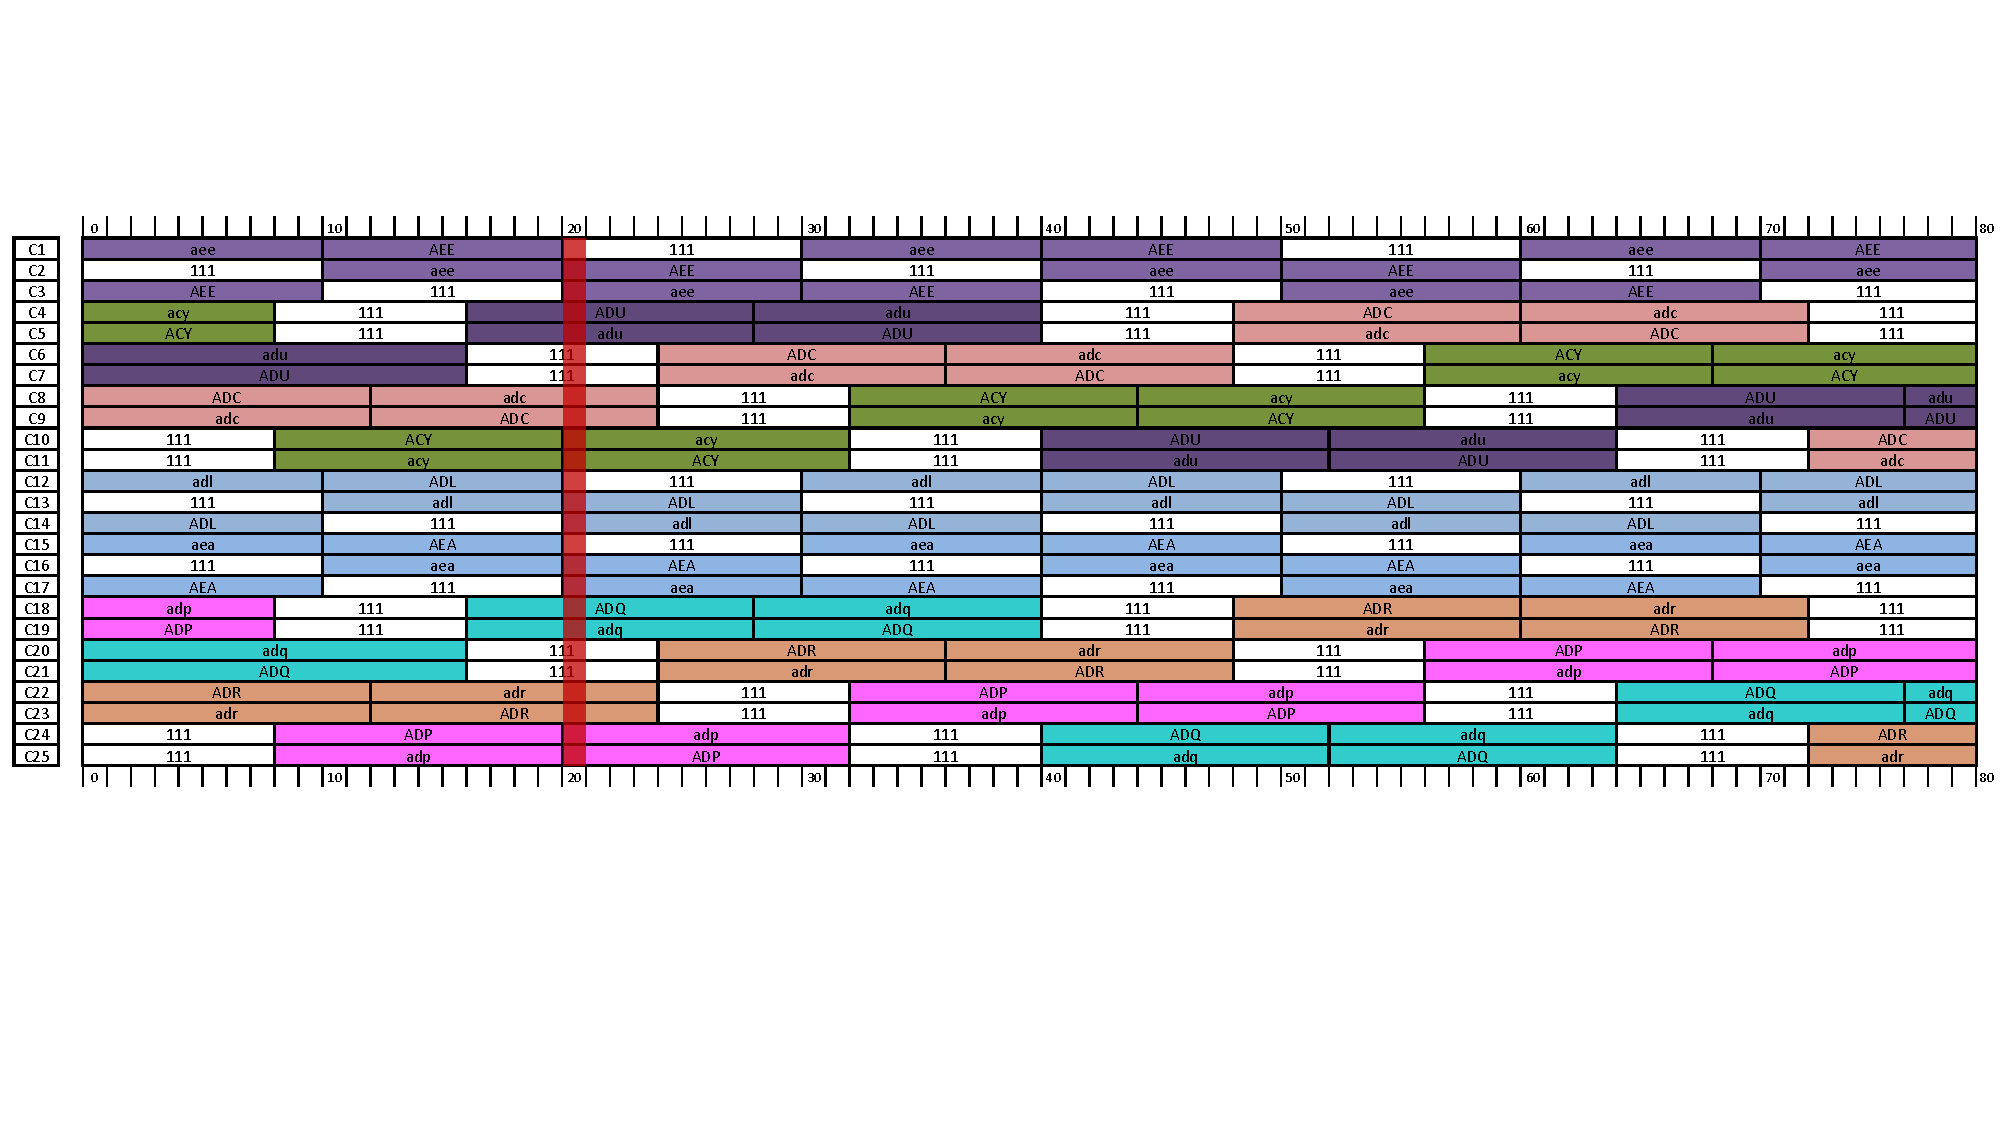
\includegraphics[width=\linewidth]{caso7/caso7-fase0}
		\caption{Planificación inicial del Caso 7}
		\label{fig:caso7-fase0}
	\end{figure}

	\begin{table}[h]
		\centering
		\caption{Sectorización inicial del Caso 7.}
		\label{table:D:caso7-inicial}
		\begin{tabular}{ccc}
			\hline
			\multicolumn{1}{c}{\textbf{Núcleo}} & \multicolumn{1}{c}{\textbf{Configuración}} & \multicolumn{1}{c}{\textbf{Intervalo}} \\ \hline
			&                                            &                                        \\
			Barcelona Ruta Este                 & 4A                                         & 15:00 -- 21:35                         \\
			Barcelona Ruta   Oeste              & 5A                                         & 15:00 -- 21:35                         \\
			\multicolumn{1}{c}{}                &                                            &                                        \\ \hline
		\end{tabular}
	\end{table}
\end{itemize}

\textbf{Momento del Cambio}: 16:40:00 (slot 20)

\textbf{Tipo incidencia}: Modificación sectorizaciones, baja de un controlador, alta de un controlador.

\textbf{Descripción}: El núcleo Este pasa de 4A a 3A, cerrándose un sector durante las últimas 1:15 horas. El núcleo Oeste se desglosa tras las primeras 1:40 horas de una 5A a 5C, que se mantiene durante 3:20 horas, luego a una 4A durante 40 minutos y finalmente 3A durante los últimos 55 minutos, como se muestra en la \autoref{table:D:caso7-modif}. Además se produce una baja del C23 a las 18:30 (slot 42) que se reemplaza con un alta de un nuevo controlador a las 20:00 (slot 60). Es necesario el uso de 4 controladores imaginario (3 para un sector, 1 para la baja del controlador).

\begin{table}[h]
	\centering
	\caption{Sectorización modificada del Caso 7.}
	\label{table:D:caso7-modif}
	\begin{tabular}{ccc}
		\hline
		\textbf{Núcleo}                                              & \textbf{Configuración} & \textbf{Intervalo} \\ \hline
		&                        &                    \\
		\multicolumn{1}{c|}{\multirow{2}{*}{Barcelona Ruta Este}}    & 4A                     & 15:00 -- 20:00     \\
		\multicolumn{1}{c|}{}                                        & 3A                     & 20:00 -- 21:35     \\
		&                        &                    \\
		\multicolumn{1}{c|}{\multirow{4}{*}{Barcelona Ruta   Oeste}} & 5A                     & 15:00 -- 16:40     \\
		\multicolumn{1}{c|}{}                                        & 5C                     & 16:40 -- 20:00     \\
		\multicolumn{1}{c|}{}                                        & 4A                     & 20:00 -- 20:40     \\
		\multicolumn{1}{c|}{}                                        & 3A                     & 20:40 -- 21:35     \\
		&                        &                    \\ \hline
	\end{tabular}
\end{table}


\subsubsection{Caso 8}

\textbf{Unidad de Control}: Palma

\textbf{Turno}: MC, 7:00 -- 15:00

\textbf{Núcleo}: Palma APP

\textbf{Situación inicial}:
\begin{itemize}[label={}]
	
	\item \textbf{Recursos}: \\
	22 PTD Palma APP \\
	
	
	\item \textbf{Sectorización}: véase la \autoref{table:5:caso8-inicial}
	
	\item Planificación inicial: véase la \autoref{fig:5:caso8-fase0}
	
	\begin{figure}[!h]
		\centering
		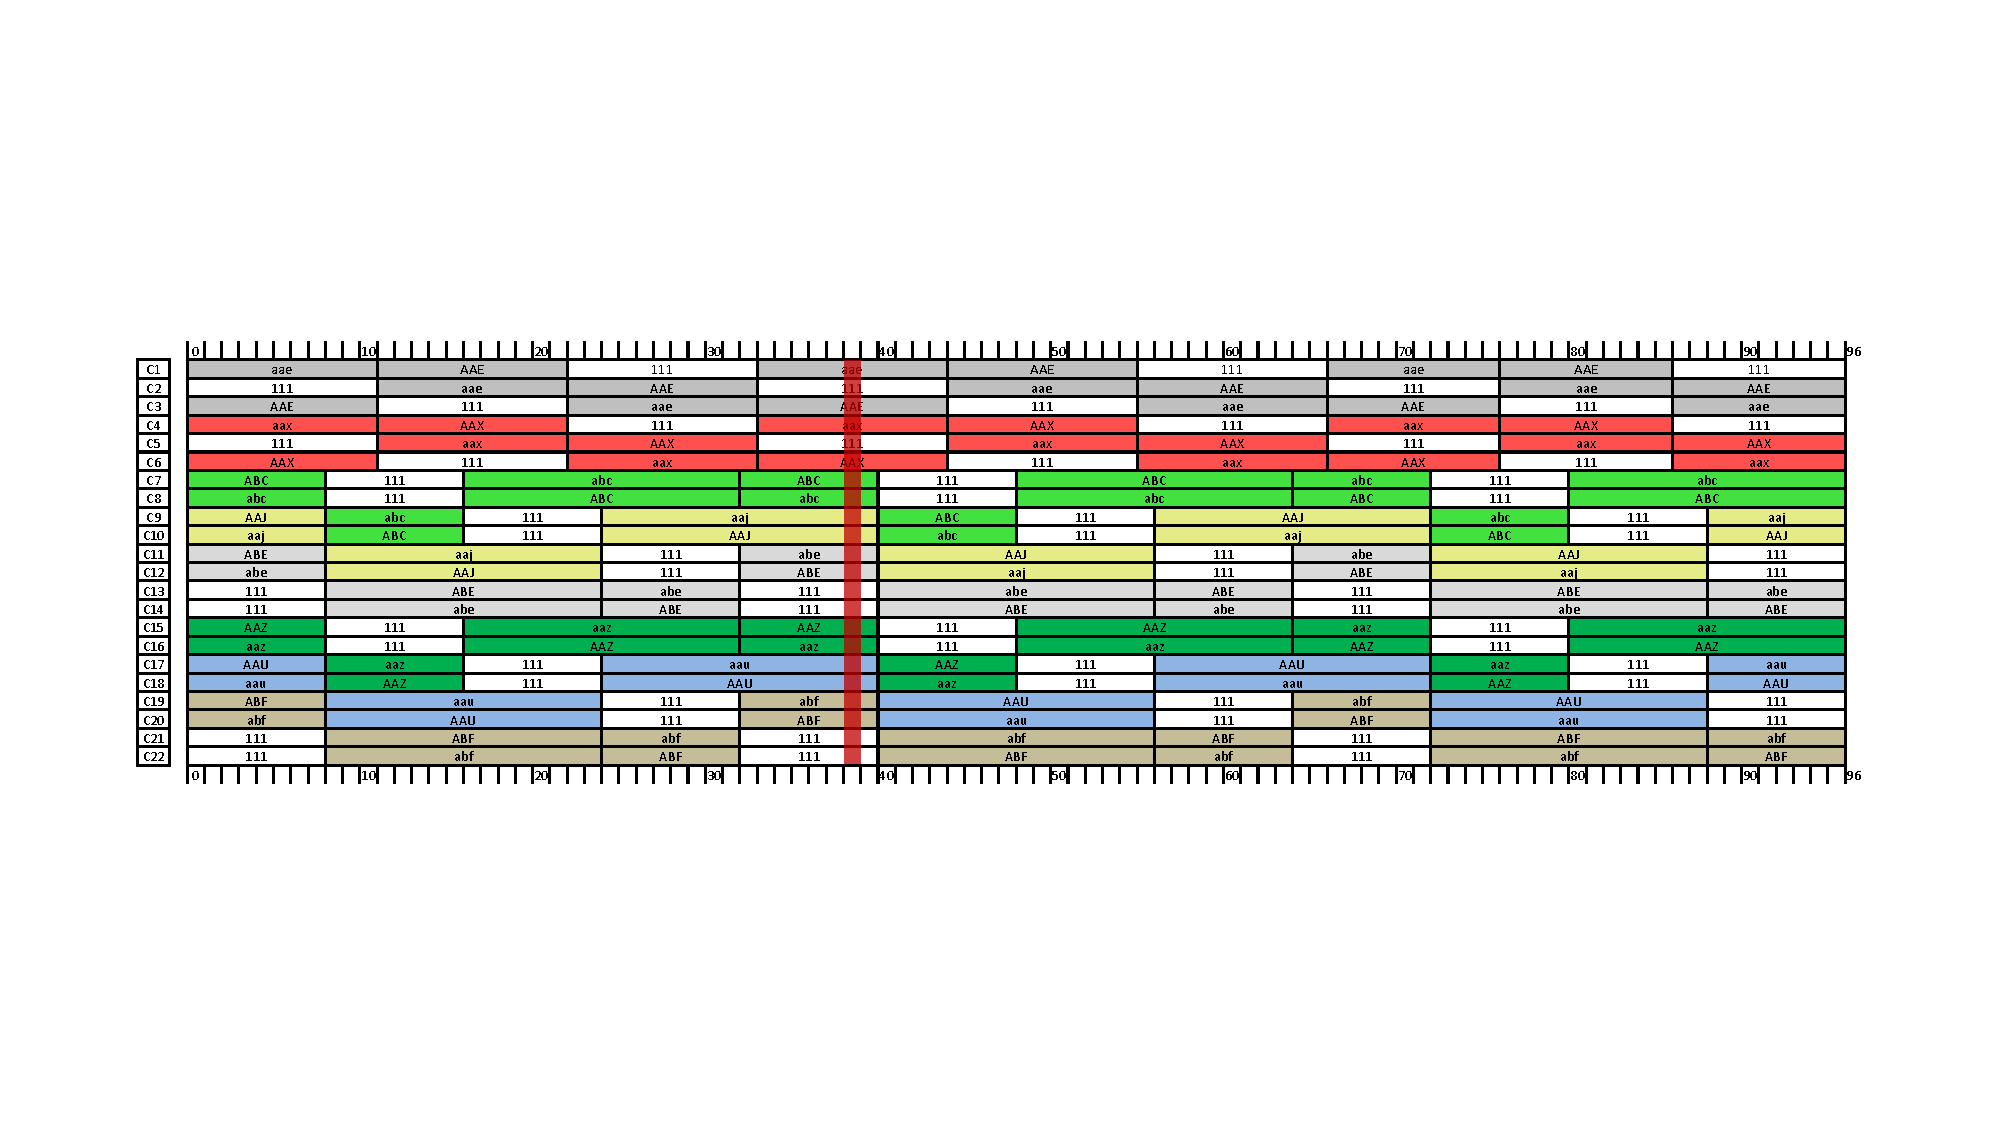
\includegraphics[width=\linewidth]{caso8/caso8-fase0}
		\caption{Planificación inicial del Caso 8}
		\label{fig:5:caso8-fase0}
	\end{figure}

	\begin{table}[h]
		\centering
		\caption{Sectorización inicial del Caso 1}
		\begin{tabular}{ccc}
			\hline
			\textbf{Núcleo}      & \textbf{Configuración} & \textbf{Intervalo}   \\ \hline
			\multicolumn{1}{l}{} & \multicolumn{1}{l}{}   & \multicolumn{1}{l}{} \\
			Barcelona Ruta Este  & 3D                     & 7:30:00--15:00:00    \\
			\multicolumn{1}{l}{} & \multicolumn{1}{l}{}   & \multicolumn{1}{l}{} \\
			Barcelona Ruta Oeste & 5A                     & 10:30:00--15:00:00   \\ \hline
		\end{tabular}
		\label{table:5:caso8-inicial}
	\end{table}
	
\end{itemize}

\textbf{Momento del Cambio}: 10:10:00 (slot 38)

\textbf{Tipo incidencia}: Baja de un controlador

\textbf{Descripción}: Se produce la baja del controlador C16 a las 10:10 (slot 38) y no es sustituido por nadie. Es necesario el uso de un controlador imaginario.


\subsubsection{Caso 9}

\textbf{Unidad de Control}: Palma

\textbf{Turno}: MC, 7:00 -- 15:00

\textbf{Núcleo}: Palma APP

\textbf{Situación inicial}:
\begin{itemize}[label={}]
	
	\item \textbf{Recursos}: \\
	22 PTD Palma APP \\
	
	\item \textbf{Sectorización}: véase la \autoref{table:5:caso8-inicial}
	
	\item Planificación inicial: véase la \autoref{fig:5:caso9-fase0}
	
	\begin{figure}[!h]
		\centering
		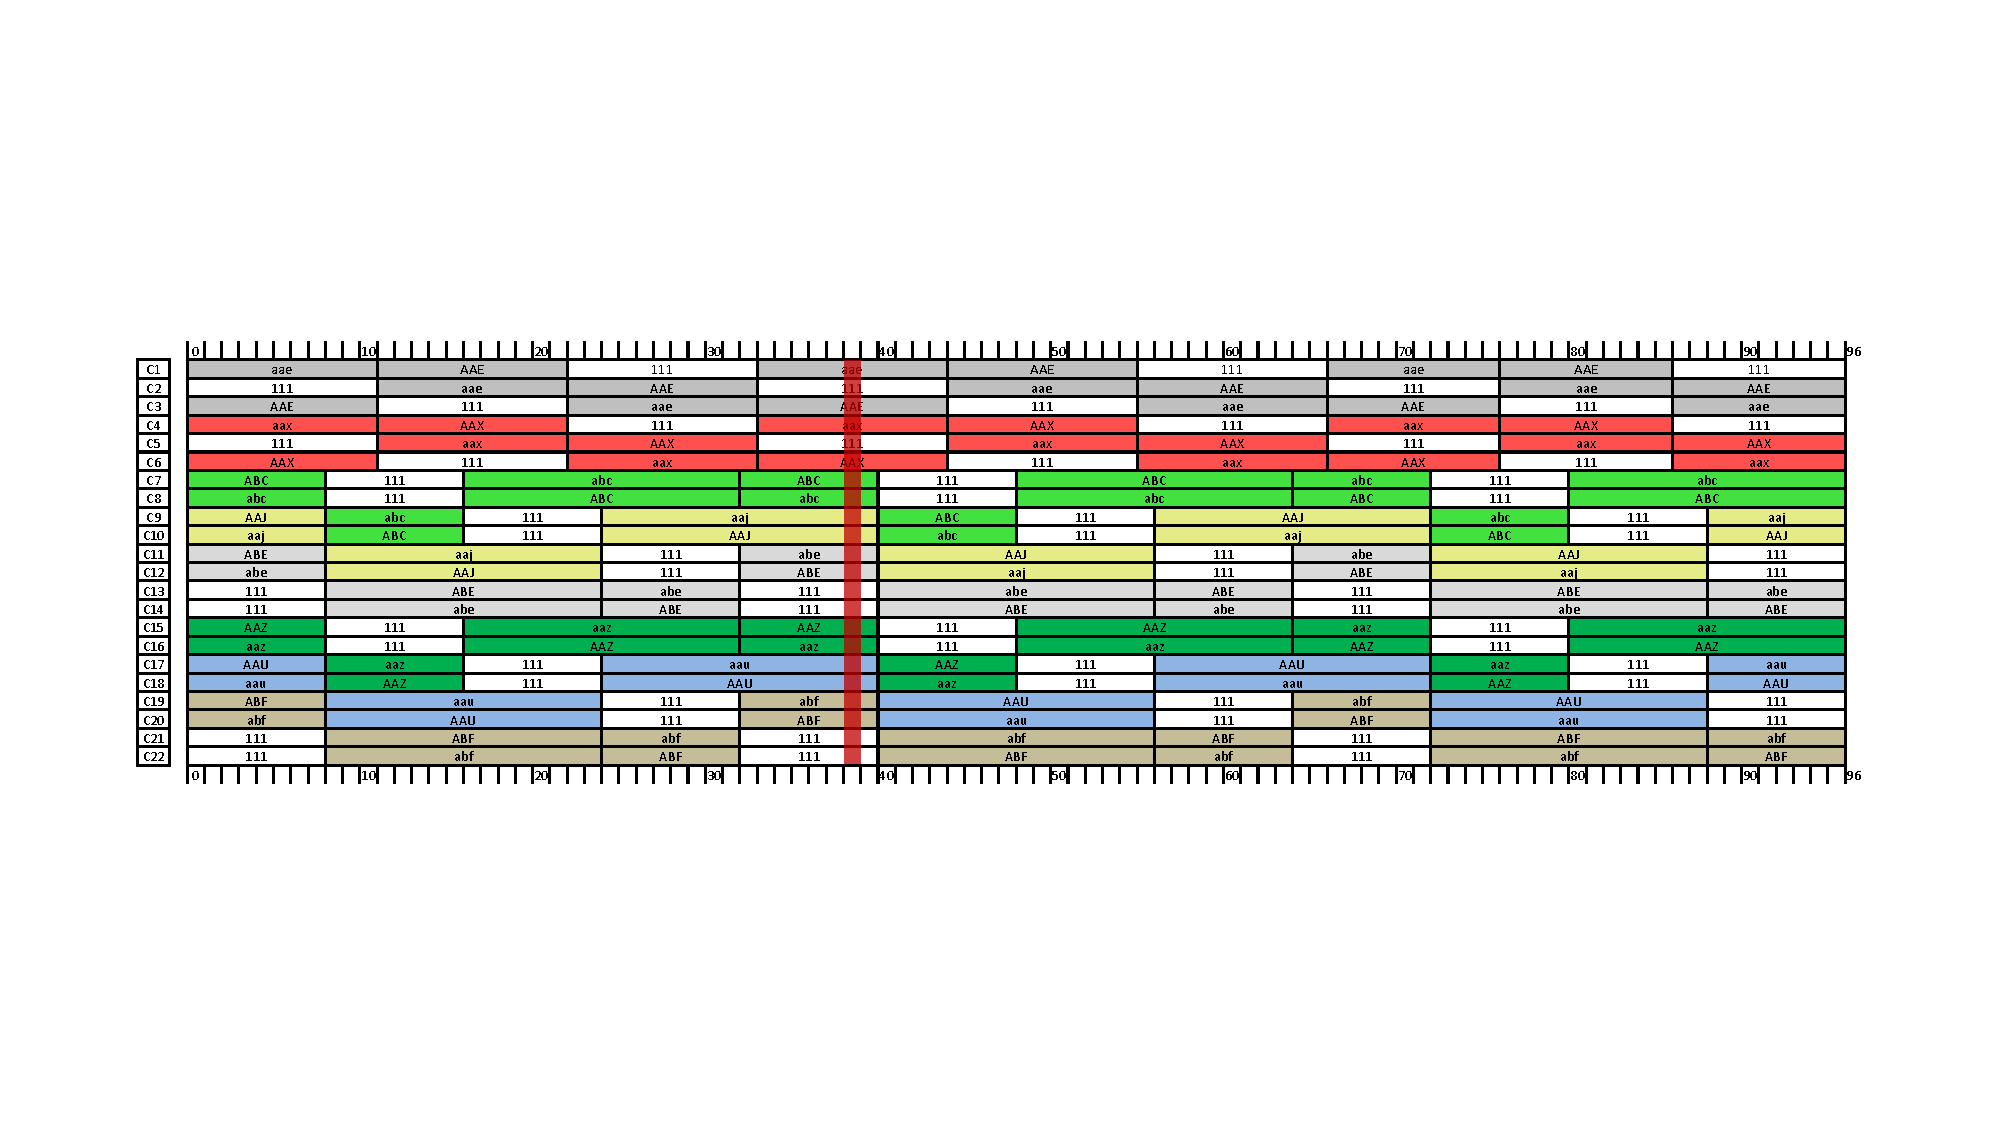
\includegraphics[width=\linewidth]{caso9/caso9-fase0}
		\caption{Planificación inicial del Caso 9}
		\label{fig:5:caso9-fase0}
	\end{figure}
	
\end{itemize}

\textbf{Momento del Cambio}: 10:10:00 (slot 38)

\textbf{Tipo incidencia}: Baja de un controlador, alta de un controlador

\textbf{Descripción}: Al igual que el Caso 8 pero la baja sí es cubierta por otro controlador a las 12:40 (2h después, slot 68). Es necesario el uso de un controlador imaginario.

\subsection{Ajuste paramétrico}
Toda metaheurística y demás sistemas de optimización tiene un conjunto de parámetros que pueden tomar un conjunto de valores posibles y que afectan activamente al rendimiento del sistema. Para poder fijar estos valores, se lleva a cambio un proceso denominado \textit{ajuste paramétrico}, o \textit{parameter tunning}, que se puede realizar de diferentes formas.

\NEW{El enfoque de inicialización \textit{off-line} consiste en fijar los valores previamente a la ejecución de la metaheurística de forma empírica para cada instancia del problema dado. Este proceso suele realizarse de forma secuencial, es decir, de uno en uno. Sin embargo, esta estrategia no considera las interacciones entre los parámetros y no garantiza hallar la configuración óptima de los mismos. Existen otras estrategias como \textit{Latin Hypercube}~\cite{latin-hypercube}, que consiste en muestrear del llamado ``Hipercubo Latino'' de tantas dimensiones como parámetros, presuponiendo que la configuración optima se encuentra en dicho cubo; limitar los valores a puntos de intersección de una cuadrícula de una granularidad dada y aproximar la localización de la configuración optima mediante el modelo estadístico de la bondad de ajuste.
Otra opción sería emplear el llamado \textit{F-Race}~\cite{F-Race}, un tipo de \textit{Racing Algorithm} que parte de un conjunto de instancias de prueba y va descartando, iterativa o factorialmente, la configuración de cada instancia cuando encuentra evidencia estadística de que la configuración es peor que al menos otra candidata~\cite{F-Race-2}. 
E incluso, podemos incluso plantear el ajuste paramétrico como otro problema de optimización a resolver mediante otra metaheurística.}

Por otro lado, se considera el enfoque de inicialización de parámetros \textit{on-line}, que permite una evolución dinámica, en tiempo de ejecución, de los valores de cada parámetro en función del rendimiento del sistema u otro criterio determinista o estocástico.

En este TFM, por ser lo más común y sencillo, se decidió emplear un enfoque \textit{off-line} de forma secuencial. Para ello, se han de ordenar los parámetros en función de su robustez, es decir, lo mucho que afecta un pequeño cambio en el parámetro al desempeño total del algoritmo. A continuación, se ajustan secuencialmente en ese orden de la siguiente manera: se fija el valor de todos los demás parámetros y se realizan ejecuciones de la metaheurística con diferentes valores para el parámetro en cuestión, y finalmente se selecciona aquel valor que mejores resultados ofrece. A continuación, se repite el proceso para el siguiente parámetro, sucesivamente.
Una vez ajustados todos los parámetros, se repite el proceso desde el principio hasta que ningún parámetro cambie de valor.

Para que los datos sean más robustos y fiables, cada configuración ha sido ejecutada un total de 10 veces y se han hecho datos medios. En el \autoref{Anexo:ejemplo-ajuste-parametrico} pueden verse con detenimiento la forma de realizar el ajuste para la instancia concreta del Caso 1.

Sin embargo, en el caso de SA ésto no fue realizado de la manera descrita. Aunque no forme parte de éste TFM, al realizar comparativas en secciones futuras describiremos brevemente el proceso de ajuste de parámetros llevado a cabo.
El objetivo del SA era realizar una búsqueda diversificada al inicio con una evolución gradual hacia la intensificación, por lo que el ajuste paramétrico se realizó mediante un análisis de las gráficas del comportamiento del proceso de búsqueda de la metaheurística, observando aquellos valores que mejor se ajustaban a ese proceso de búsqueda deseado.

% ALFONSO SAID:
% Empieza por aquel parámetro que creas que es menos robusto, es decir, aquel que al realizar un pequeño cambio en el parámetro pueda hacer que cambie significativamente el desempeño del algoritmo. Una vez que determines su valor más adecuado, lo fijas y analizas el segundo parámetro menos robusto. Una vez que determines su valor más adecuado, lo fijas y analizas el tercer parámetro menos robusto. Y así sucesivamente, hasta el último y vuelves a empezar para realizar otro ciclo hasta que los parámetros no cambien o cambien muy poco. Siempre cambias un parámetro, nunca realices cambios en más de un parámetro a la vez.

\subsubsection{Parámetros del sistema} \label{sec:5:parametros-sistema}
Los parámetros del sistema, descritos anteriormente en la \autoref{sec:3:metaheurística}, ordenados por su robustez son:
\begin{enumerate}
	\item Tipo de VNS
	\begin{enumerate}[label={},left=-1pt]
		\item Para skewed:
	\end{enumerate}
	\begin{enumerate}[label*={\arabic*}]
		\item $\alpha$
		\item Función de distancia 
	\end{enumerate}
	\item Estructuras de vecindad y orden
	\item Naturaleza del orden de los entornos (determinísticos o probabilísticos)
	\begin{enumerate}[label={},left=-1pt]
		\item Para Probabilístico:
	\end{enumerate}
	\begin{enumerate}[label*={\arabic*}]
		\item Probabilidad de diversificación
		\item Variación de la probabilidad de diversificación 
		\item Número de iteraciones sin variar la probabilidad de diversificación 
	\end{enumerate}
	\item Número de iteraciones para comprobar el porcentaje de mejoría (ciclos)
	\item Porcentaje mínimo de mejoría
	\item Número máximo de iteraciones sin mejora para la búsqueda local
	\item Porcentaje mínimo de mejoría para la búsqueda local
\end{enumerate}

En el proceso de ajuste paramétrico se han empleado, para cada uno de los parámetros, los valores iniciales recogidos en la \autoref{table:5:valores-parametros-iniciales}.

\begin{table}[h]
	\centering
	\caption{Valores iniciales empleados para el ajuste paramétrico}
	\label{table:5:valores-parametros-iniciales}
	\begin{tabular}{llcl}
		\hline
		& Parámetro       & Valor inicial &  \\ \hline
		& \quad \quad 1               &      VND      &  \\
		& \quad \quad 1.1             &       5       &  \\
		& \quad \quad 1.2             &   por slots   &  \\
		& \quad \quad 2               &      (b)      &  \\
		& \quad \quad 3               & Determinista  &  \\
		& \quad \quad 3.1             &      0.9      &  \\
		& \quad \quad 3.2             &      0.1      &  \\
		& \quad \quad 3.3             &       5       &  \\
		& \quad \quad 4               &     5 000     &  \\
		& \quad \quad 5               &     0.035     &  \\
		& \quad \quad 6               &       5       &  \\
		& \quad \quad 7               &       0       &  \\ 
		& Semilla inicial &      20       &  \\ \hline
	\end{tabular}
\end{table}


Para el parámetro relativo al orden de los entornos se ha usado la siguiente nomenclatura:

\begin{enumerate}[label={(\alph*)}]
	\item movRejilla, movMaxCarga\_1, movMaxCarga\_2, movMaxCarga\_3, movMaxCarga\_4, movLibre
	\item movMaxCarga, movRejilla\_1, movRejilla\_2, movRejilla\_3, movRejilla\_4, movLibre
	\item movMaxCarga\_1, movMaxCarga\_2, movMaxCarga\_3, movMaxCarga\_4, movRejilla\_1, movRejilla\_2, movRejilla\_3, movRejilla\_4, movLibre
	\item movRejilla\_1, movRejilla\_2, movRejilla\_3, movRejilla\_4, movMaxCarga\_1, movMaxCarga\_2, movMaxCarga\_3, movMaxCarga\_4, movLibre
\end{enumerate}


\subsubsection{Análisis de los resultados del ajuste}
\label{sec:5:resultados-ajuste}

El proceso que nos ocupa fue realizado siguiendo el procedimiento descrito anteriormente, obteniéndose los resultados que se encuentran recogidos en la \autoref{table:5:tunning-results}. Por límites espaciales, se han empleado los números identificativos asignados en la sección anterior.

\begin{table}[h]
	\centering
	\caption{Resultados del ajuste paramétrico.}
	\label{table:5:tunning-results}
	\resizebox{\textwidth}{!}{%
		\begin{tabular}{lcccccccc}
			\hline
			Parámetro &        Caso 1        &        Caso 3        &        Caso 4        &        Caso 5        &        Caso 6        &        Caso 7        &        Caso 8        &        Caso 9        \\ \hline
			1         &         VND          &         VND          &         BVNS         &         BVNS         &         VND          &         VND          &         BVNS         &         BVNS         \\
			1.1       &          -           &          -           &          -           &          -           &          -           &          -           &          -           &          -           \\
			1.2       &          -           &          -           &          -           &          -           &          -           &          -           &          -           &          -           \\
			2         &         (b)          &         (b)          &         (d)          &         (c)          &         (d)          &         (c)          &         (c)          &         (b)          \\
			3         &     Determinista     &     Determinista     &     Determinista     &    Probabilístico    &     Determinista     &     Determinista     &     Determinista     &    Probabilístico    \\
			3.1       &          -           &          -           &          -           &         0.7          &          -           &          -           &          -           &         0.1          \\
			3.2       &          -           &          -           &          -           &        0.001         &          -           &          -           &          -           &        0.005         \\
			3.3       &          -           &          -           &          -           &          5           &          -           &          -           &          -           &          5           \\
			4         &        30 000        &        45 000        &        10 000        &        45 000        &        6 000         &        40 000        &        20 000        &        25 000        \\
			5         &        0.015         &         0.1          &         0.01         &        0.005         &         0.3          &        0.015         &        0.005         &         0.05         \\
			6         &          1           &          3           &          20          &          5           &          5           &          5           &          20          &          5           \\
			7         &         0.5          &          0           &          1           &          0           &         0.05         &        0.005         &         0.01         &         0.1          \\ \hline
			          & \multicolumn{1}{l}{} & \multicolumn{1}{l}{} & \multicolumn{1}{l}{} & \multicolumn{1}{l}{} & \multicolumn{1}{l}{} & \multicolumn{1}{l}{} & \multicolumn{1}{l}{} & \multicolumn{1}{l}{}
		\end{tabular}%
	}
\end{table}

Como puede verse, por lo general la implementación de VNS que mejores resultados alcanza para la mayoría de los casos es su versión más sencilla: el \textit{VND}. No obstante, encontrarnos cuatro casos en los que la variante Basic, \textit{BVNS}, aporta resultados significativamente mejores en las soluciones que logra alcanzar el sistema. Sin embargo, tal y como muestra la \autoref{fig:caso4-tipo-orden-tiempo} las variaciones no suelen ser muy grandes entre sí, a excepción del \textit{SVNS}, que es el que peores resultados obtiene.

\begin{figure}
	\centering
	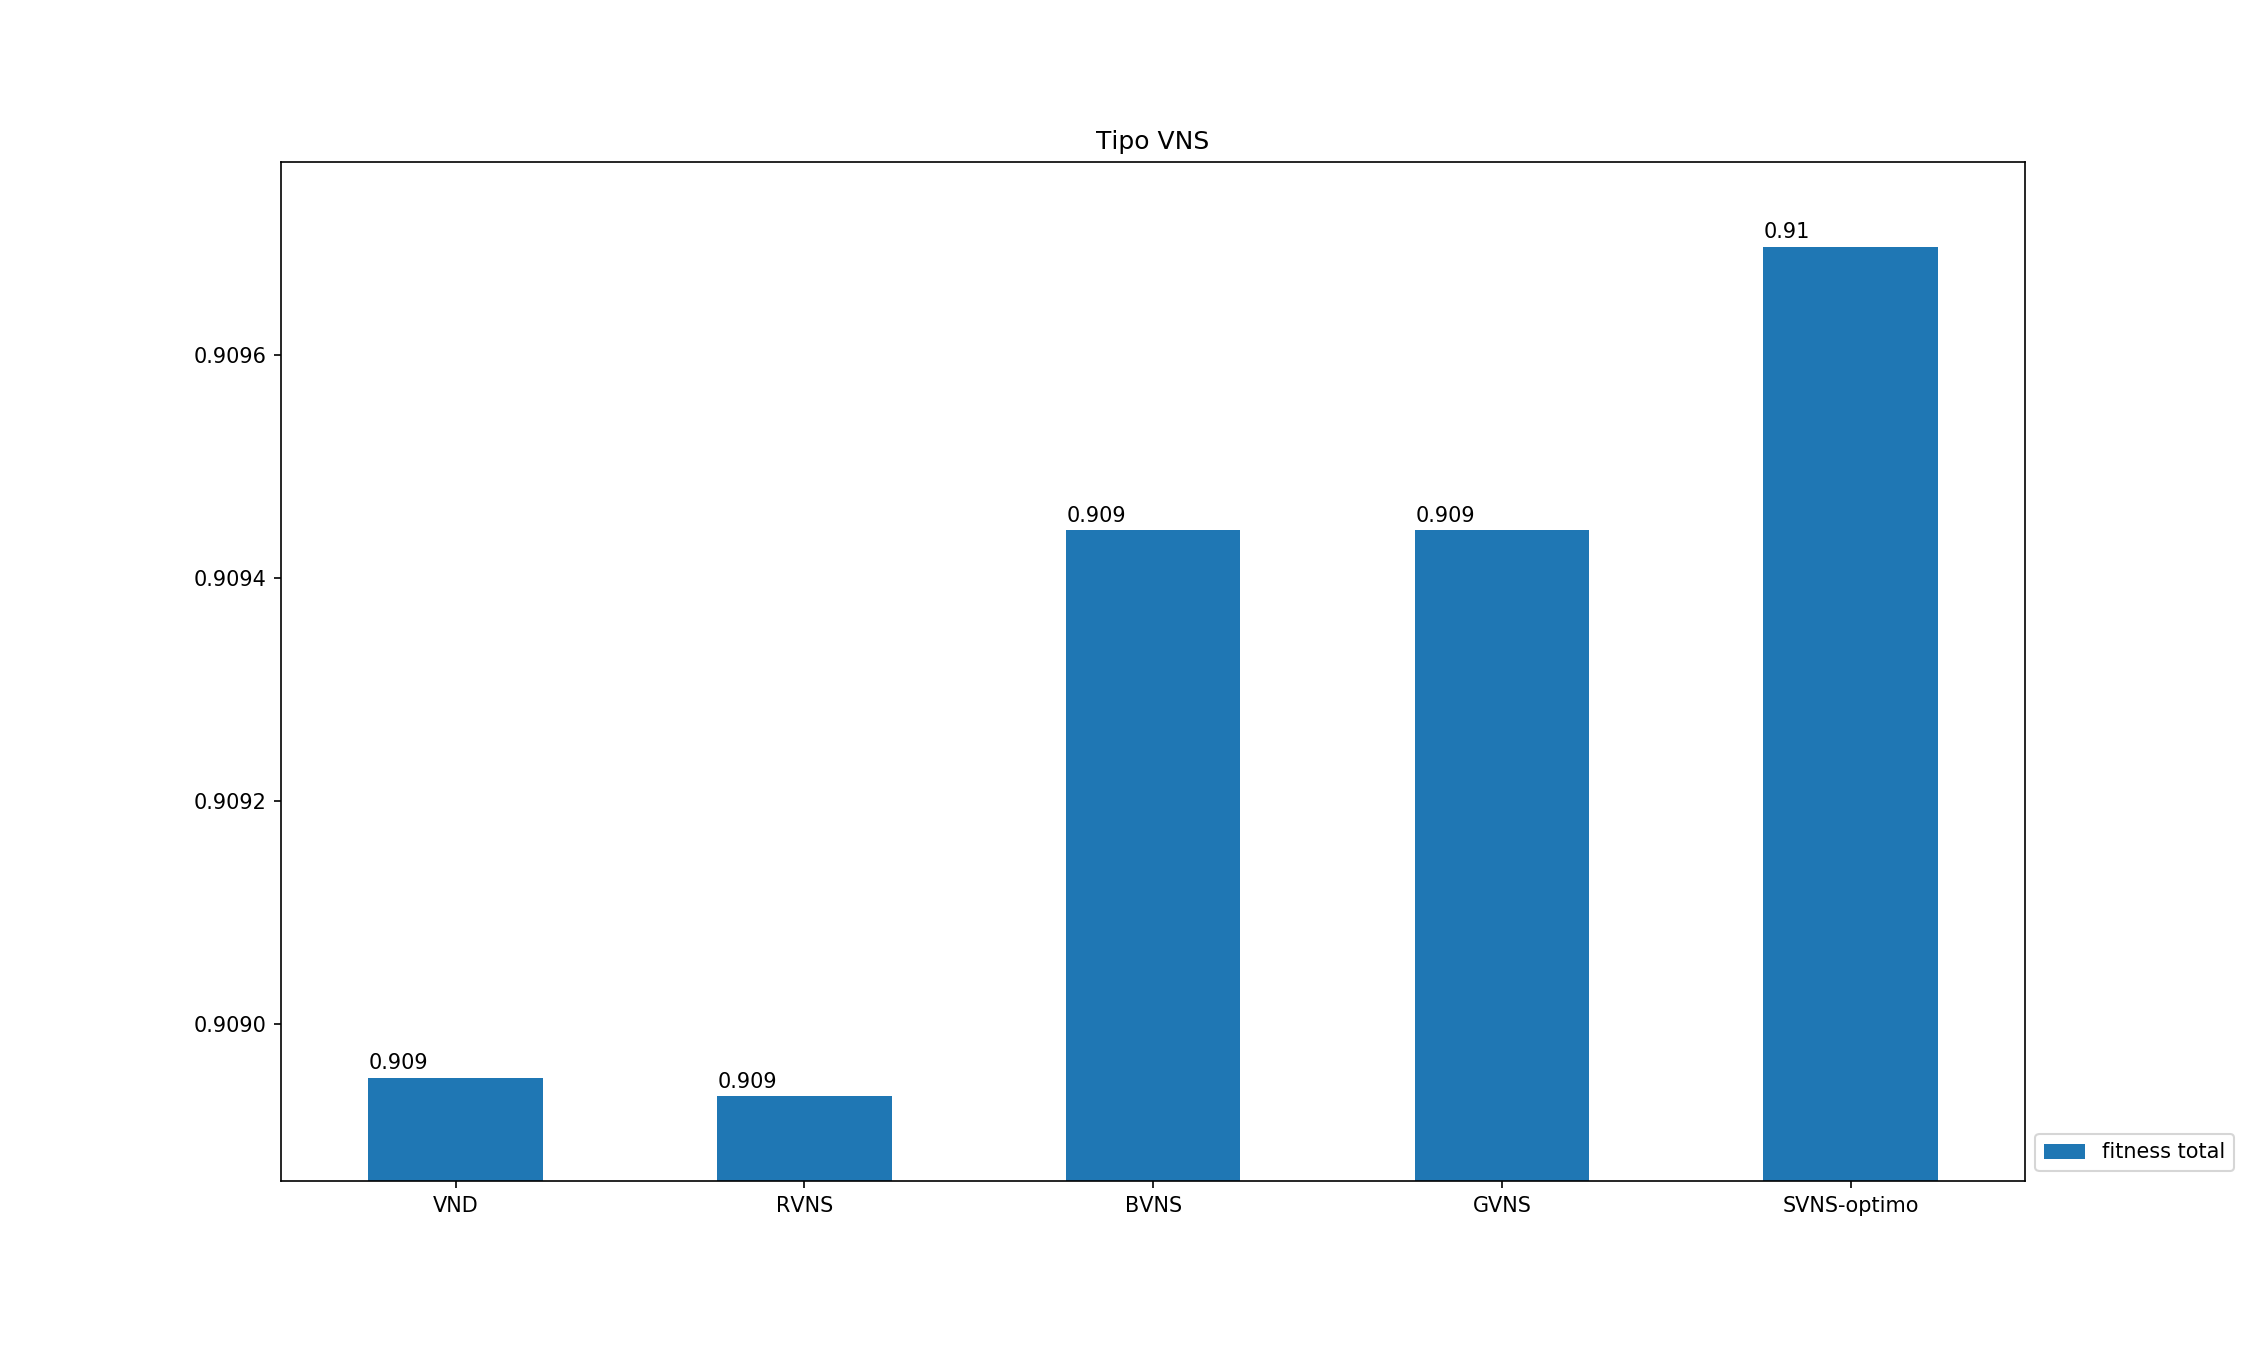
\includegraphics[width=\linewidth]{caso4-tipo-orden-tiempo}
	\caption{Variación del fitness según el tipo de VNS para el Caso 4. Ordenado según el tiempo de ejecución de cada uno}
	\label{fig:caso4-tipo-orden-tiempo}
\end{figure}

Sin embargo, esta mejora se obtiene a costa de una mayor necesidad de tiempo de cómputo, con una diferencia de $31.2762$ segundos para el Caso 4 del \textit{BVNS} frente al \textit{VND}. Sin duda, hemos observado que el \textit{RVND} es el tipo de VNS que menos tiempo de cómputo requiere, pero suele ser el que peores resultados alcanza después del \textit{SVNS}. 

La \autoref{fig:caso4-tipo-orden-tiempo} ofrece adicionalmente un ranking donde nos muestra de forma ordenada los tipos de VNS que más tiempo consumen. Como era de esperar, el \textit{SVNS} y el \textit{GVNS} son los más costosos, mientras que el \textit{VND} y \textit{RVNS} los que menos. Por su parte, el \textit{GVNS} y el \textit{BVNS} dan resultados que en la mayoría de los casos son muy similares entre sí, a excepción de en el Caso 1 y el 3, donde los resultados son más dispares. En aquellos casos donde ha habido empate, se ha optado por usar la versión menos costosa computacionalmente, que es el \textit{BVNS}.

En la \autoref{fig:caso4y9comparativa-tipos-vnsiteracion} podemos observar la evolución por iteraciones de cada VNS, donde podemos apreciar cómo, a diferencia del resto, el \textit{SVNS} no es estrictamente creciente, aceptando soluciones peores. La línea \textit{SVNS-óptimo} señala la mejor solución alcanzada hasta el momento por el \textit{SVNS}, que como podemos ver, no alcanza resultados tan buenos como los del resto. Cada ejecución termina cuando se alcanza la condición de parada del porcentaje mínimo de mejora. Además, el desempeño del \textit{BVNS} y el \textit{GVNS} es el mismo en ambos casos, aunque esto no siempre sucede en todas las iteraciones ni en todos los casos.

\begin{figure}
	\begin{subfigure}{\linewidth}
		\centering
		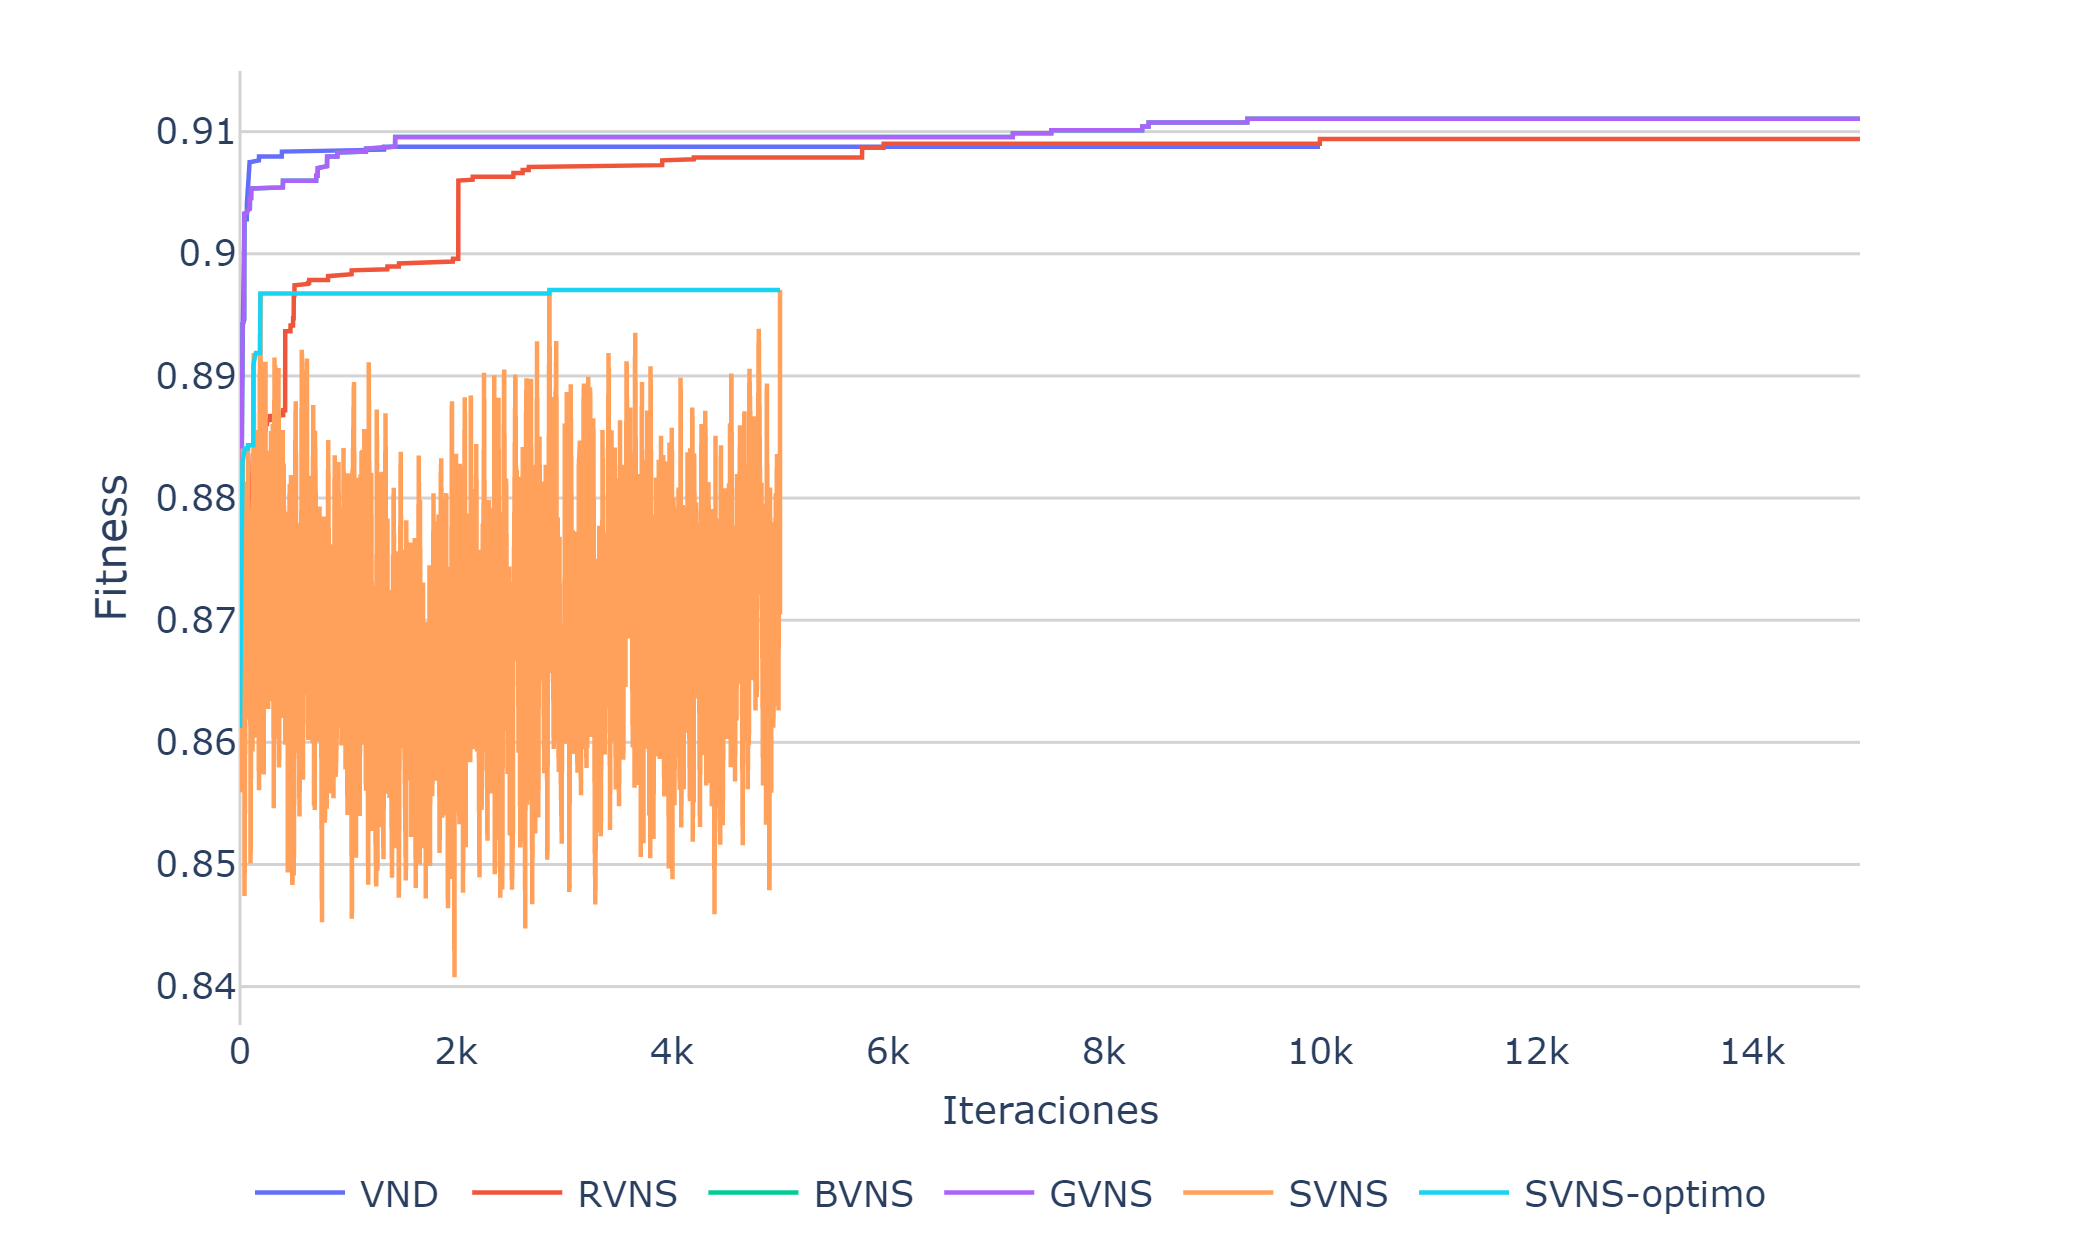
\includegraphics[width=\linewidth]{Caso4_comparativa-tipos-vns_iteracion}
		\caption{Caso 4}
		\label{fig:caso4comparativa-tipos-vnsiteracion}
	\end{subfigure}

	\begin{subfigure}{\linewidth}
		\centering
		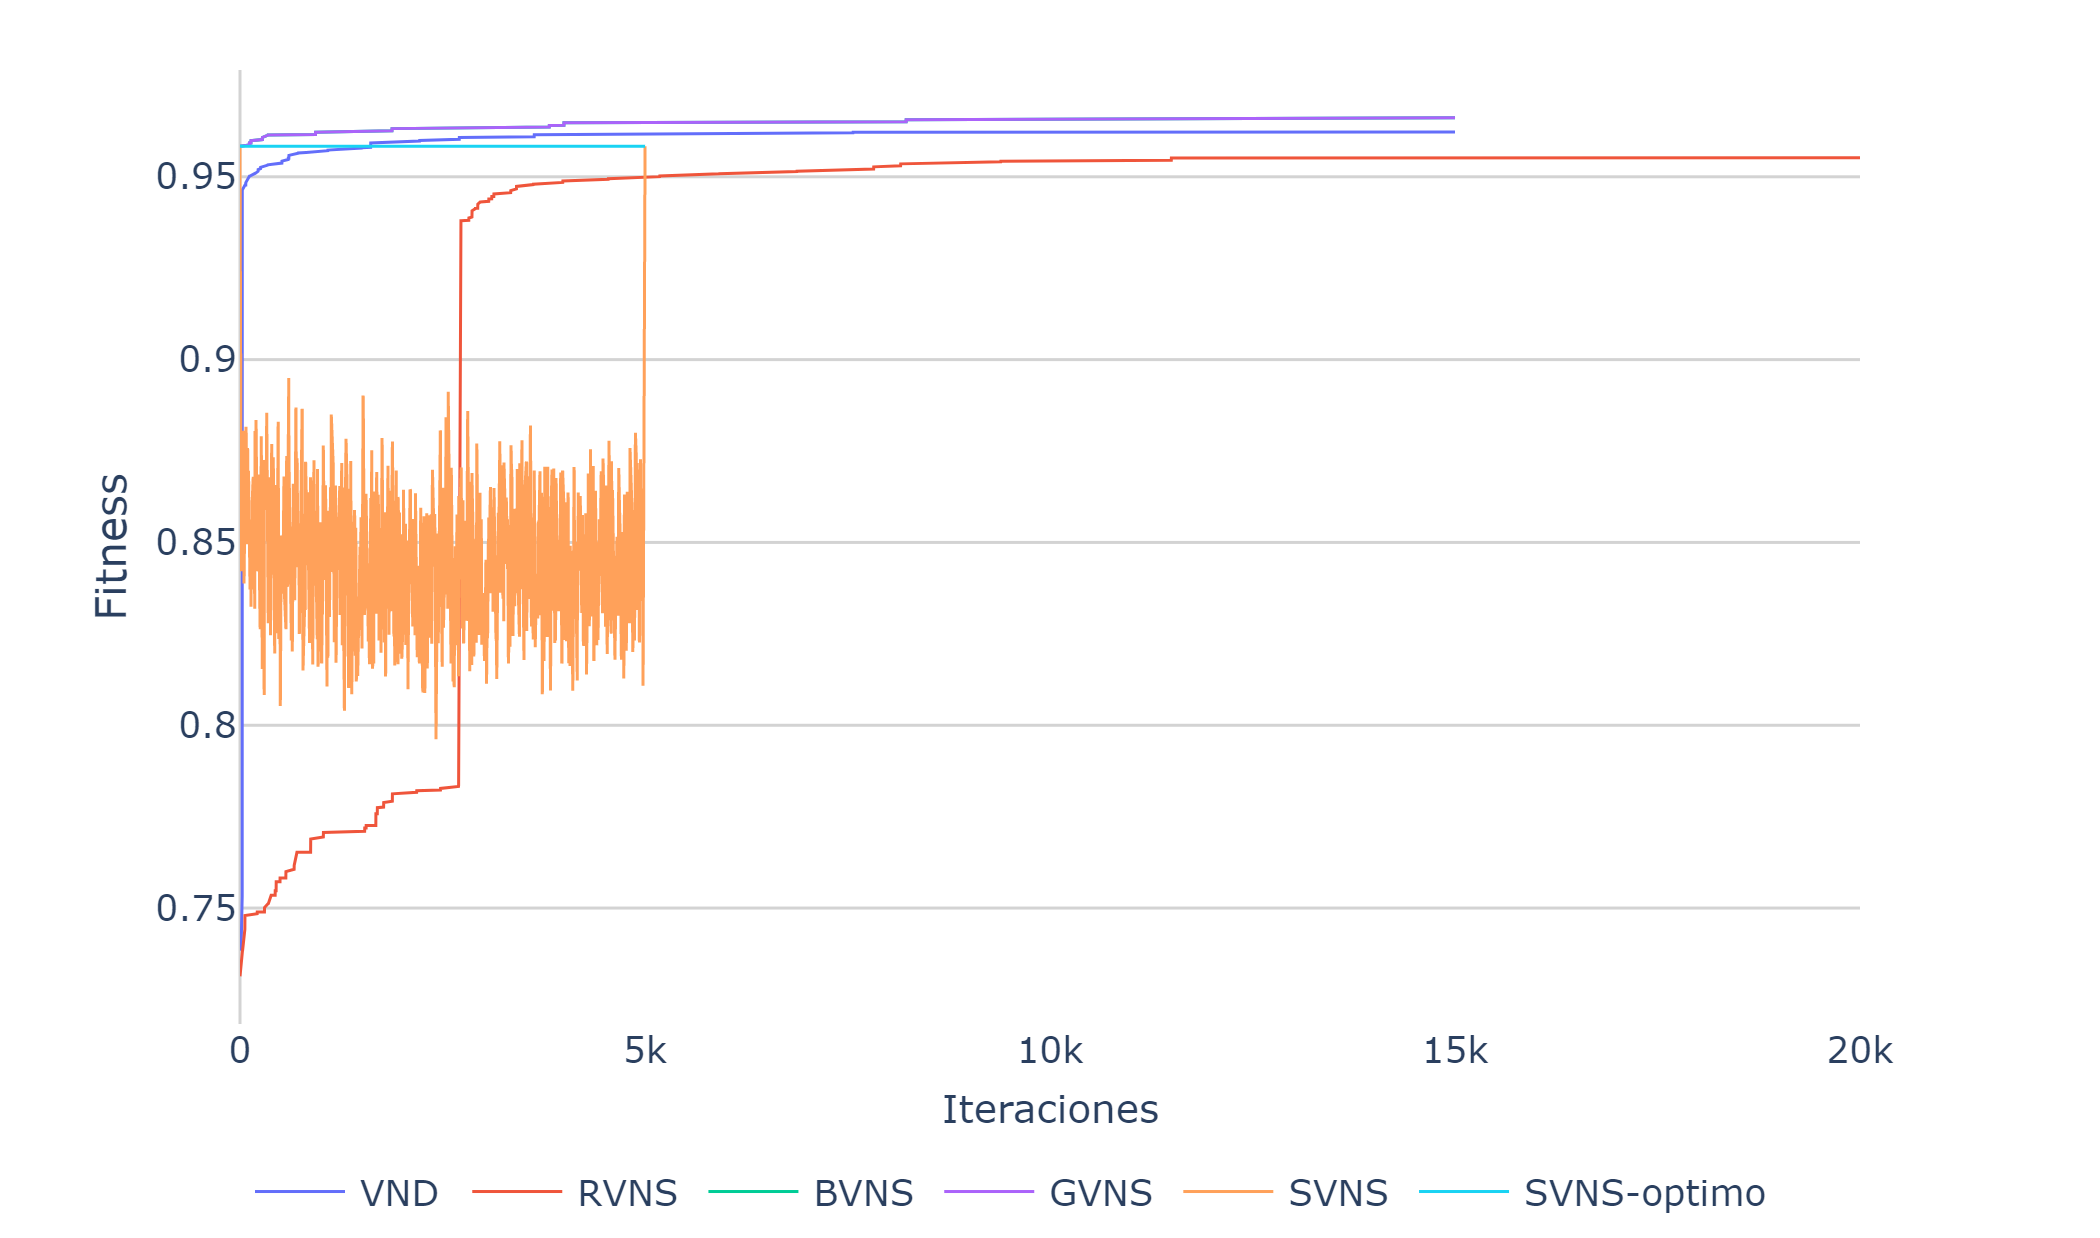
\includegraphics[width=\linewidth]{Caso9_comparativa-tipos-vns_iteracion}
		\caption{Caso 9}
		\label{fig:caso9comparativa-tipos-vnsiteracion}
	\end{subfigure}
	\caption[Evolución de cada tipo de VNS para una ejecución concreta del Caso 4 y 9.]{Evolución de cada \textbf{tipo de VNS} para una ejecución concreta del Caso 4 y 9.}
	\label{fig:caso4y9comparativa-tipos-vnsiteracion}
\end{figure}

En cuanto al orden de los entornos, no hay una clara tendencia, pero sí observamos que el primero planteado, (a), es el menos efectivo, puesto que sus resultados son superados por otros. Por otro lado, la selección óptima de los mismos es claramente determinista, salvo en el Caso 5 y 9. 
La comparativa es estos dos casos nos dice que diferencia entre determinista y probabilístico en cuanto a resultados obtenidos no es demasiado grande, del orden de una milésima (véase la \autoref{fig:caso5-naturaleza-entornos}) aunque para este caso concreto, con la opción probabilística, el número de restricciones incumplidas en la solución final es menos disperso que en la determinista, es decir, la diferencia entre una ejecución u otra no es tan grande como en el caso de la determinista. No obstante, para el resto de casos esta dispersión no sucede de una forma tan significativa.

\begin{figure}
	\centering
	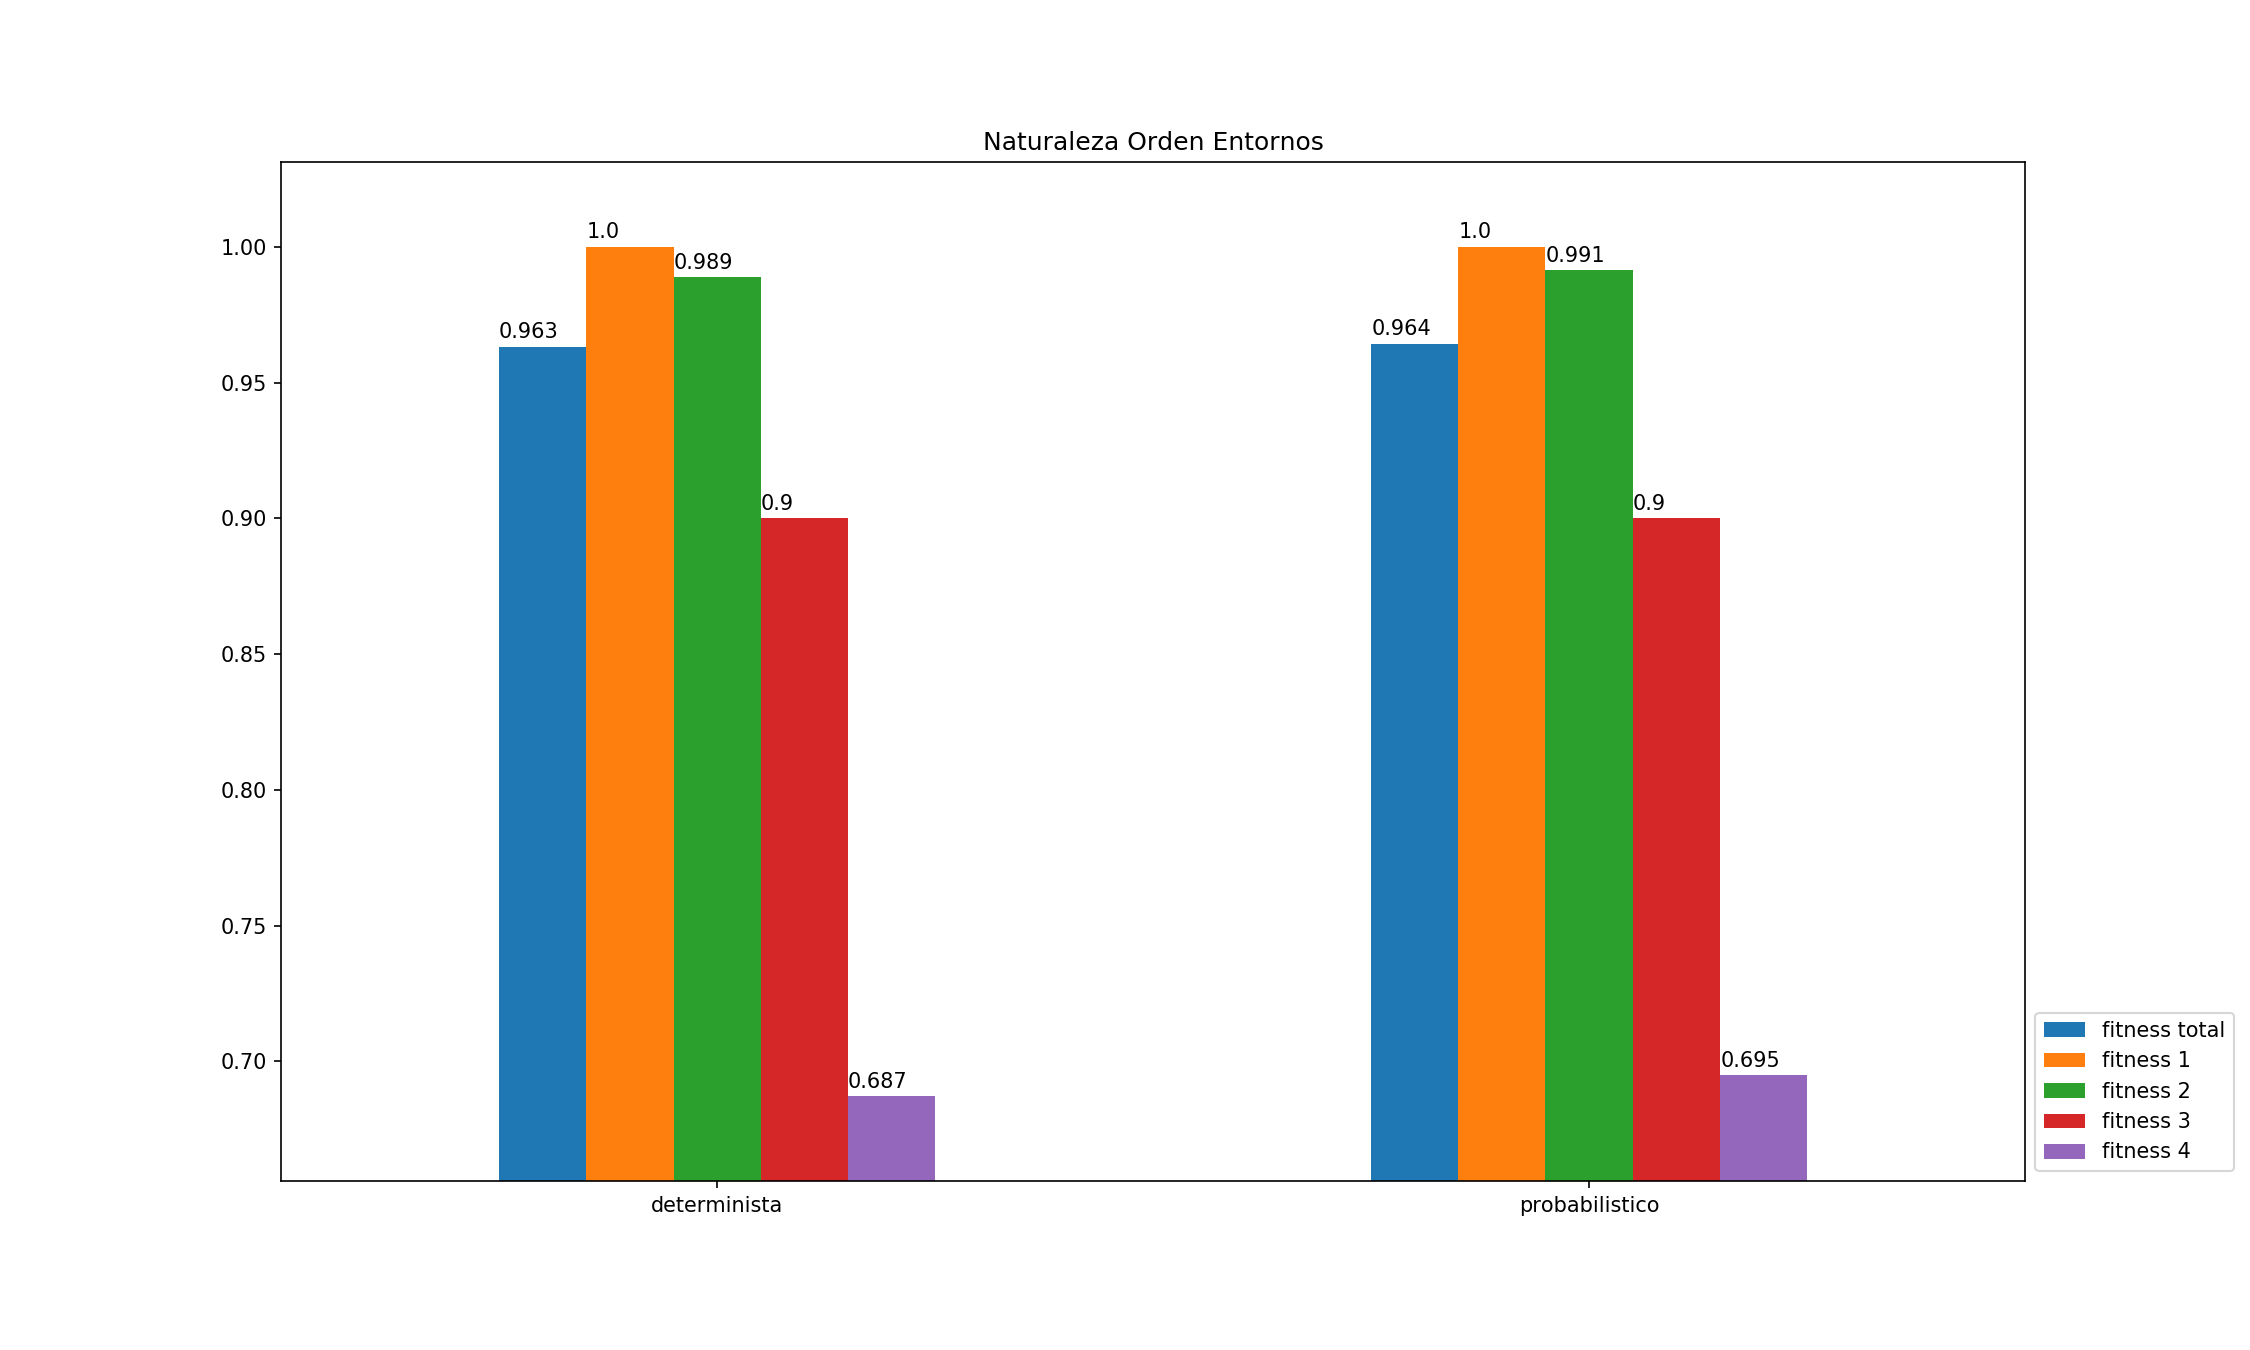
\includegraphics[width=1\linewidth]{caso5-naturaleza-entornos}
	\caption[Comparación desglosada por valor de cada objetivo para el tipo de cambio de entorno en el Caso 5]{Comparación desglosada por valor de cada objetivo para el \textbf{tipo de cambio de entorno} en el Caso 5.}
	\label{fig:caso5-naturaleza-entornos}
\end{figure}

En la \autoref{fig:caso4y9determinista-vs-probabilisticoiteracion} podemos observar la evolución de una ejecución, comparando el desempeño de sistema para cambios de entorno de tipo determinista y de tipo probabilístico, una vez seleccionados los parámetros óptimos relativos a este último. Se aprecia cómo, para el Caso 9  (\autoref{fig:caso9determinista-vs-probabilisticoiteracion}), la diferencia es significativa: el probabilístico aporta lo suficiente como para ser utilizado. Sin embargo, para el Caso 4~(\autoref{fig:caso4determinista-vs-probabilisticoiteracion}) el tipo de cambio de entornos determinista supera al probabilístico pero por muy poca diferencia.

\begin{figure}
	\begin{subfigure}{\linewidth}
		\centering
		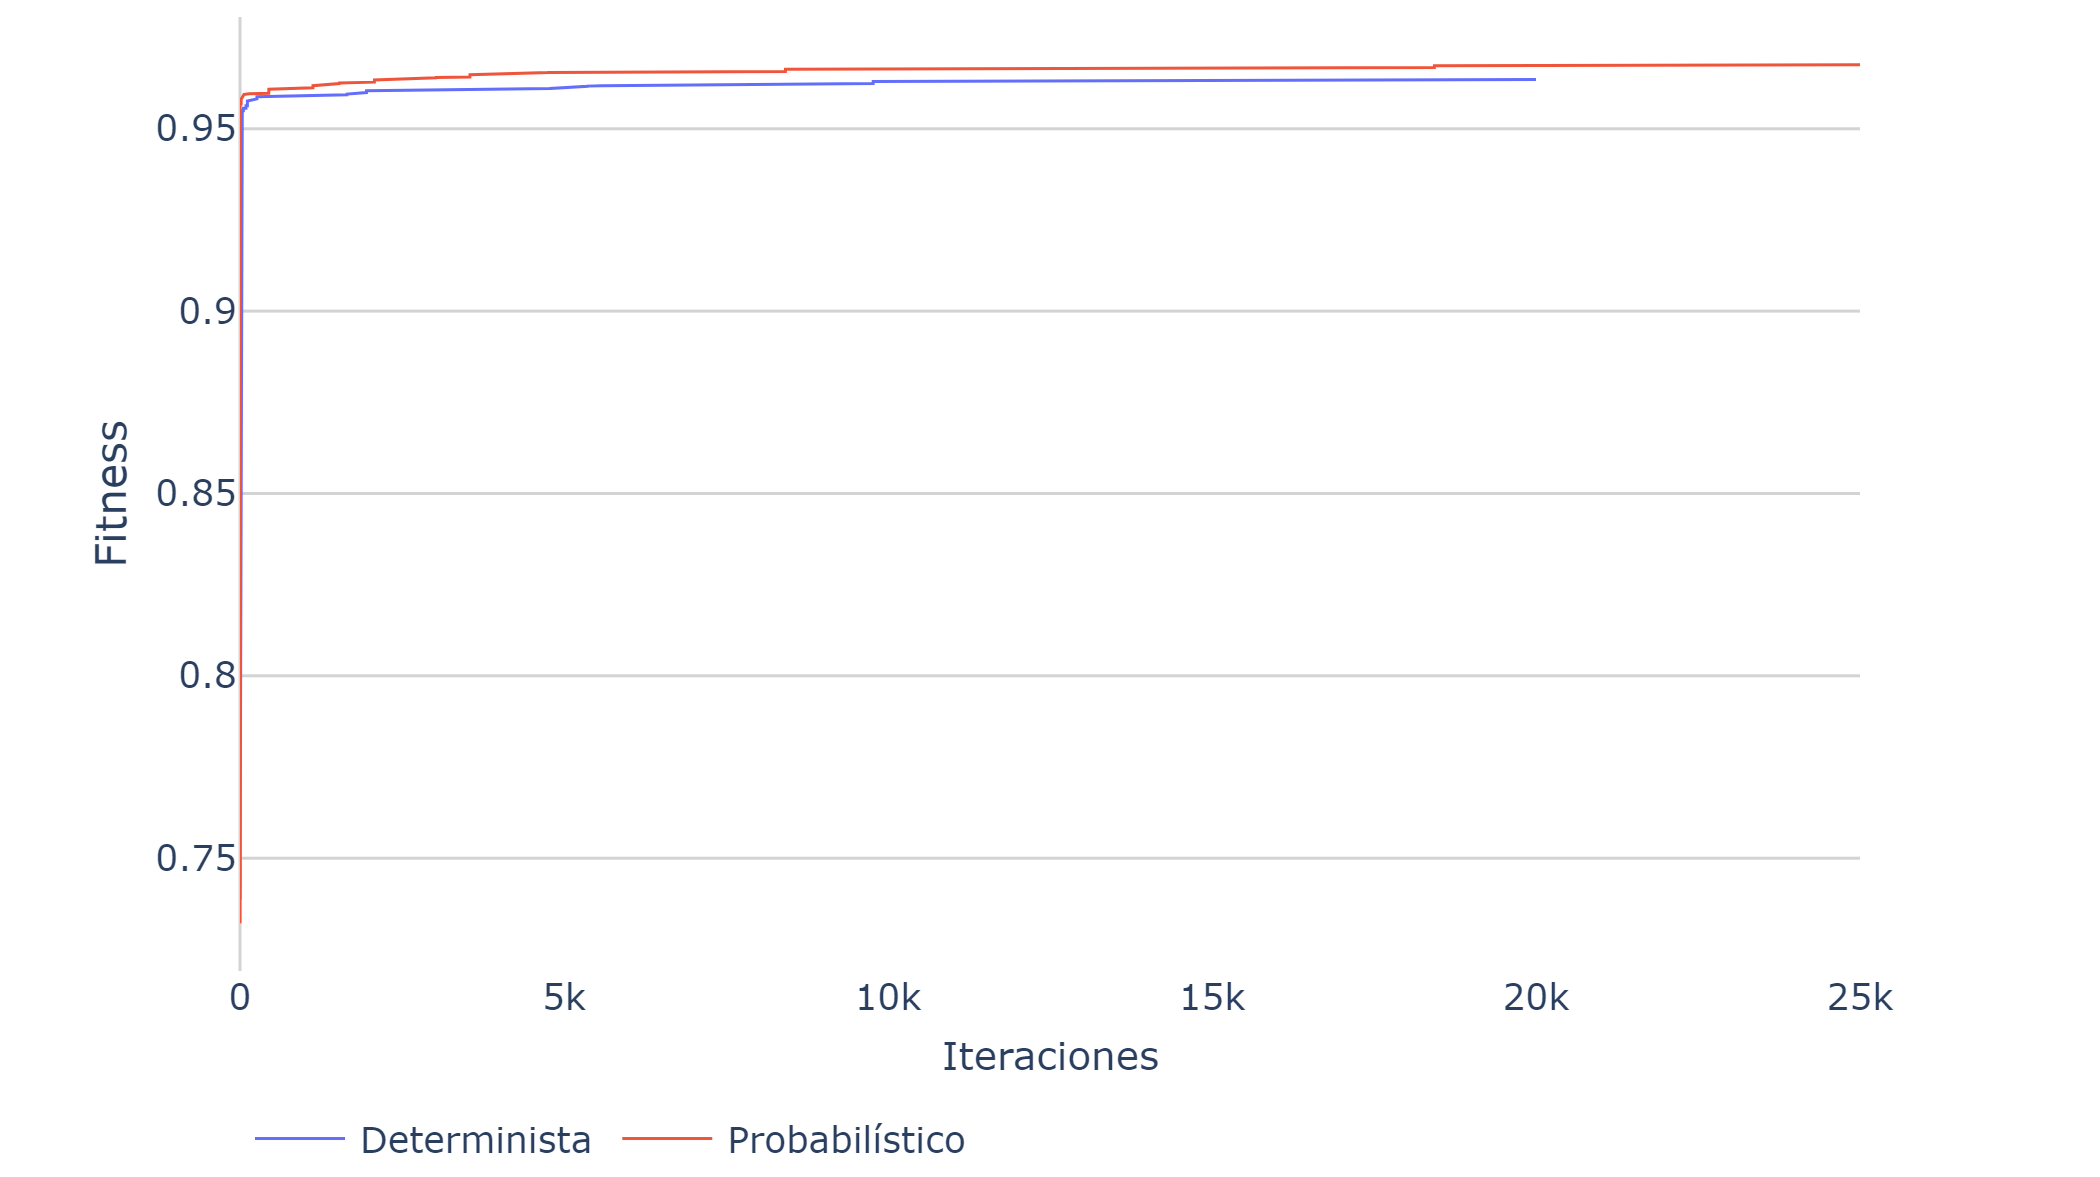
\includegraphics[width=1\linewidth]{Caso9_determinista-vs-probabilistico_iteracion}
		\caption{Caso 9}
		\label{fig:caso9determinista-vs-probabilisticoiteracion}
	\end{subfigure}

	\begin{subfigure}{\linewidth}
		\centering
		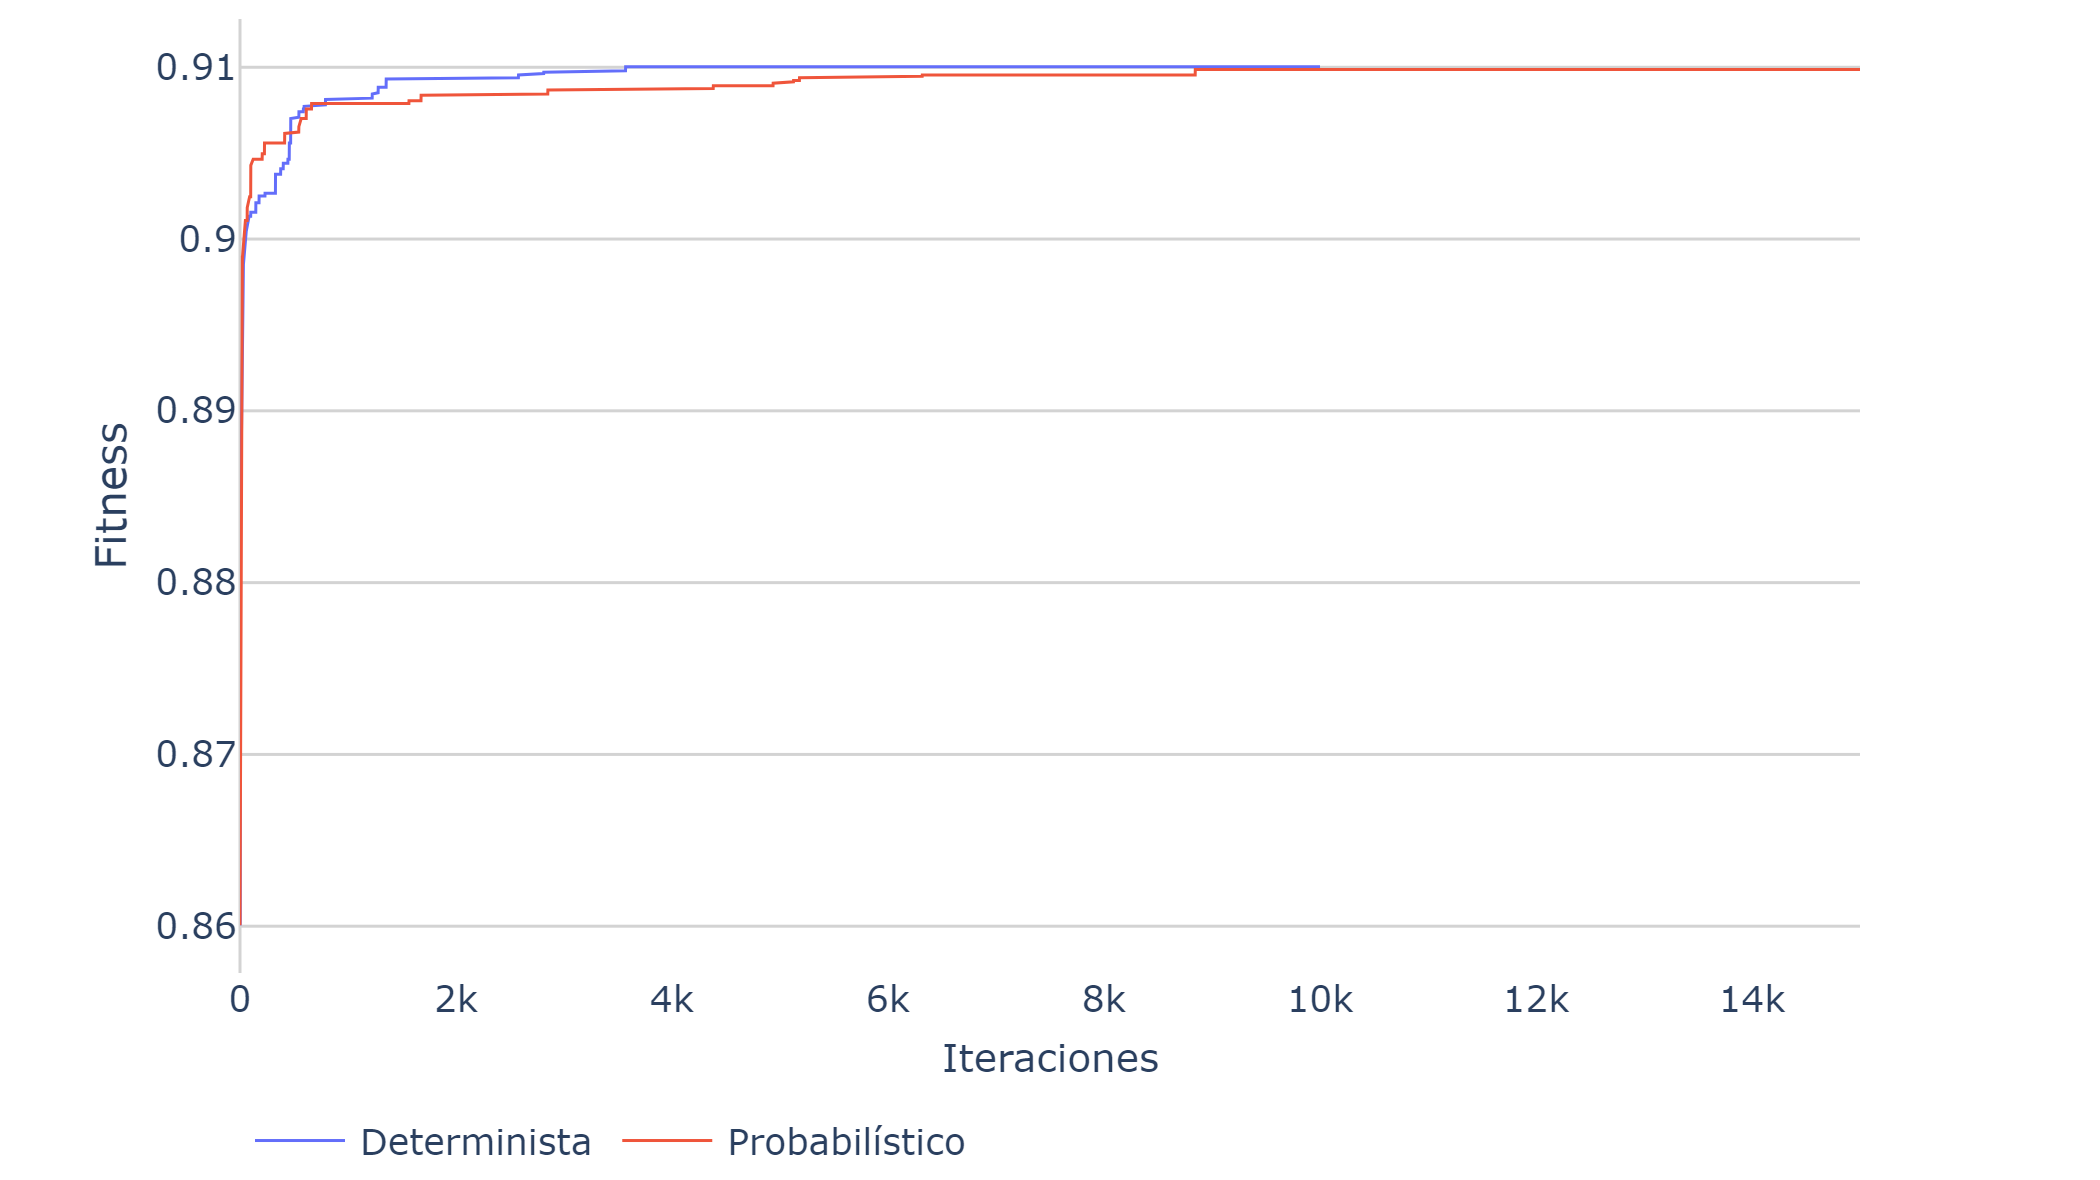
\includegraphics[width=1\linewidth]{Caso4_determinista-vs-probabilistico_iteracion}
		\caption{Caso 4}
		\label{fig:caso4determinista-vs-probabilisticoiteracion}
	\end{subfigure}
	\caption[Evolución del sistema para una ejecución concreta del Caso 9 y 4 con cambios de entorno de tipo determinista o probabilístico]{Evolución del sistema para una ejecución concreta del Caso 9 y 4 con \textbf{cambios de entorno} de tipo determinista o probabilístico.}
	\label{fig:caso4y9determinista-vs-probabilisticoiteracion}
\end{figure}


%Observamos que los parámetros óptimos que afectan a la modalidad probabilista de los entornos se adecuan al VNS en cuanto a que, por ejemplo emplear una probabilidad inicial de $0.7$ con una variación pequeña, en lugar de una probabilidad de 1, pues el número de iteraciones no es suficientemente grande como para que 

En cuanto a los demás parámetros, no hay diferencias importantes entre sí. El número de iteraciones que conforman el ciclo mínimo para comprobar la condición de parada se mueven entre $6\,000$ y $45\,000$. Para su elección fue tomado en cuenta no solo el valor de la función fitness, sino también el tiempo empleado, buscando un equilibrio entre ambos, pues como muestra la \autoref{fig:5:caso3-numero-iteraciones-para-comprobar-porcentaje-mejoria}, cuanto mayor es el número de iteraciones por ciclo, mayor es el valor de fitness hasta un punto en el que se estabiliza. No obstante, hay ocasiones en las que el crecimiento es especialmente lento o más estable, como sucede en el Caso 5 o 6. En esos casos, se ha optado por buscar el mencionado equilibrio, en el que el tiempo no fuese demasiado grande.

\begin{figure}
	\centering
	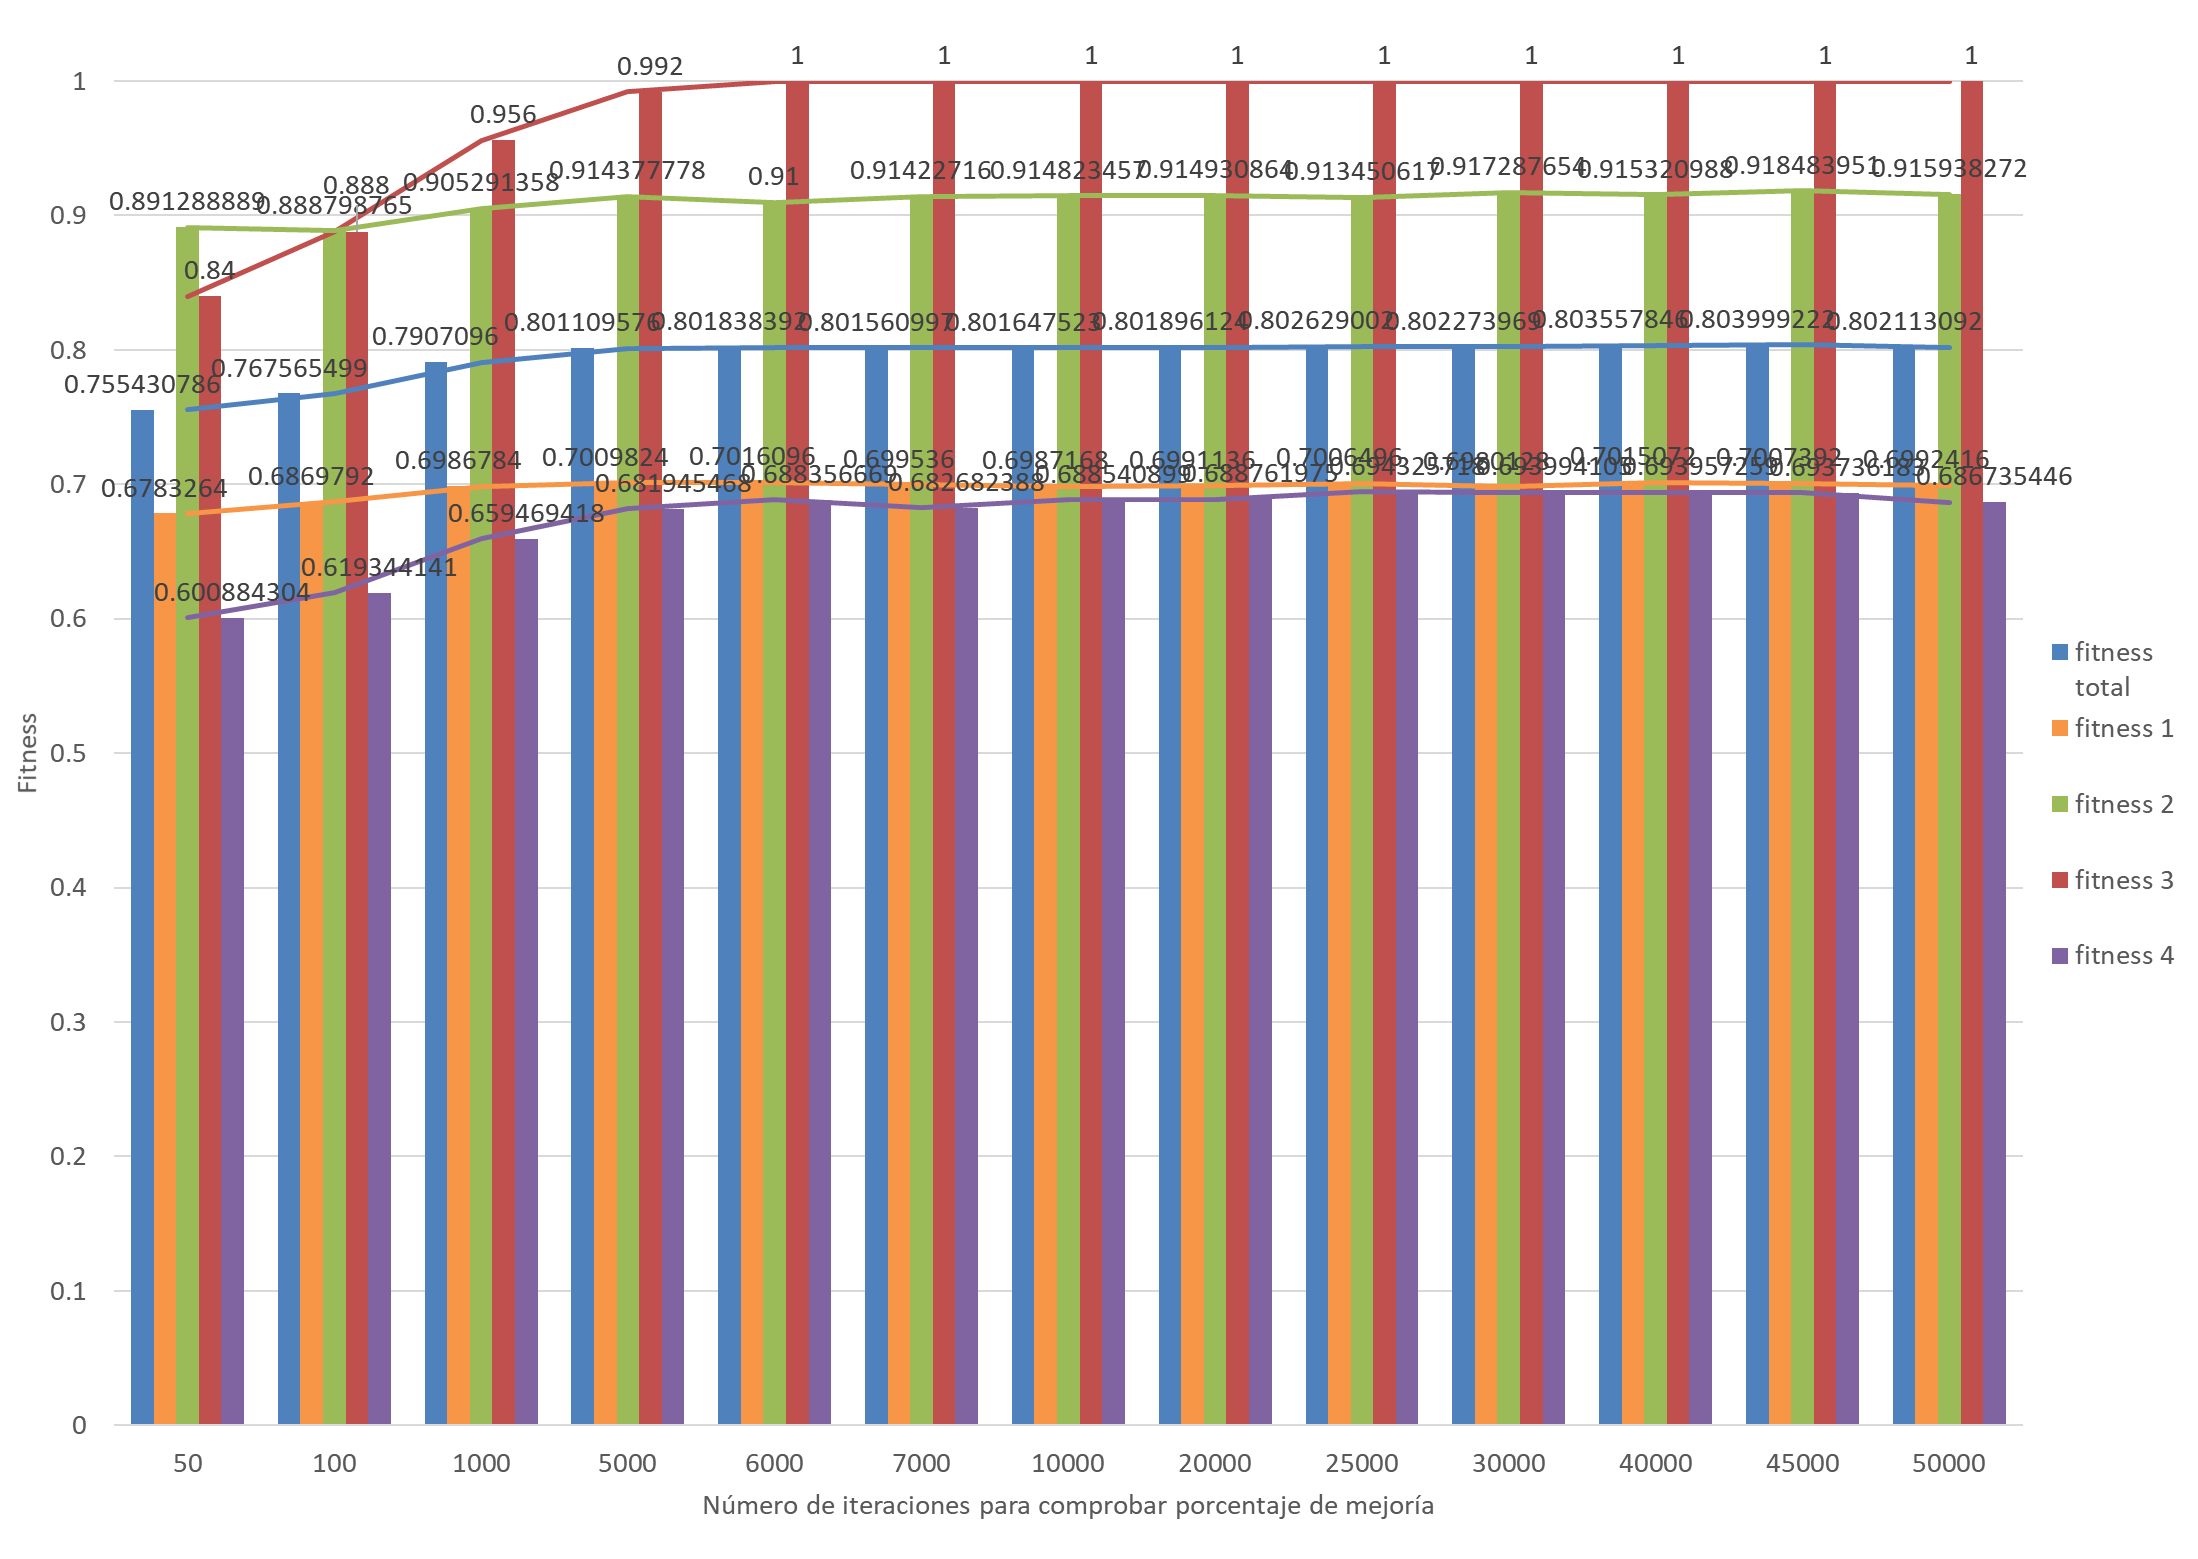
\includegraphics[width=\linewidth]{grafica-caso3-numero-iteraciones-para-comprobar-porcentaje-mejoria-maxi2}
	\caption{Variación del valor de fitness desglosado para diferentes valores del parámetro del número de iteraciones para comprobar el porcentaje de mejoría del Caso 3.}
	\label{fig:5:caso3-numero-iteraciones-para-comprobar-porcentaje-mejoria}
\end{figure}




La función de distancia aplicada para el \textit{SVNS} que mejores resultados alcanza es aquella que calcula el número de slots dispares entre ambas soluciones. Hemos observado que el valor del parámetro $\alpha$ óptimo oscila entre 0.5 y 2, y para tamaños superiores a 2, o bien deja de admitir soluciones peores, o bien se comporta de la misma forma que con otros valores inferiores. En la \autoref{fig:caso9comparativa-alphasiteracion0-5} podemos observar cómo se comporta la metaheurística \textit{SVNS} con diferentes $\alpha$ para el Caso 9, si bien exploran de diferentes formas, no logran mejorar significativamente los resultados iniciales, aunque esto sí sucede aunque muy levemente, para el Caso 3, como muestra la \autoref{fig:Caso3_comparativa-alphas_iteracion}.

\begin{figure}
	\begin{subfigure}{\linewidth}
	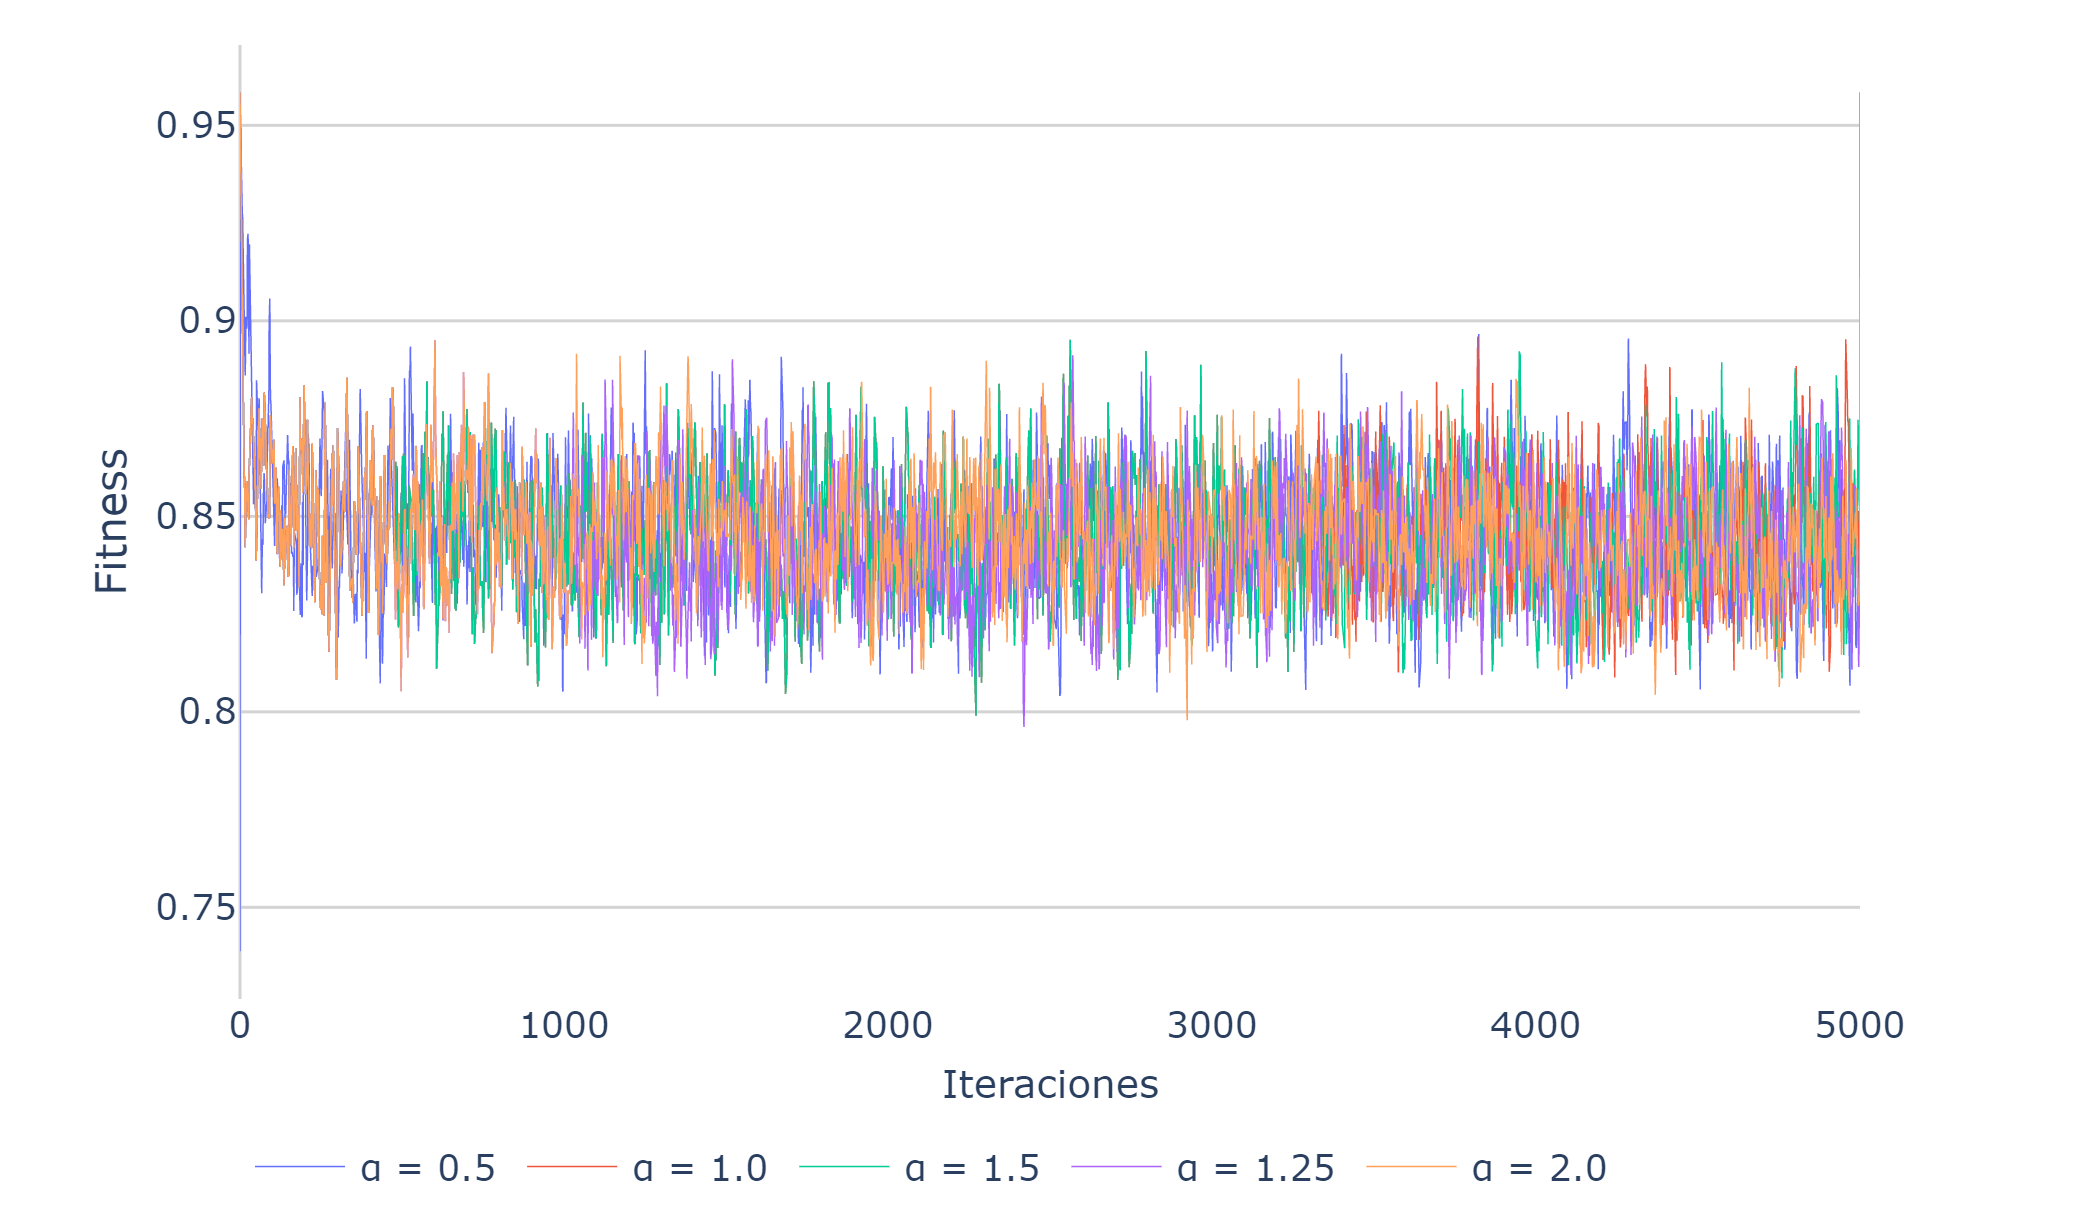
\includegraphics[width=\linewidth]{Caso9_comparativa-alphas_iteracion_0-5}
	\caption{Caso 9}
	\label{fig:caso9comparativa-alphasiteracion0-5}
	\centering
	\end{subfigure}

	\begin{subfigure}{\linewidth}
	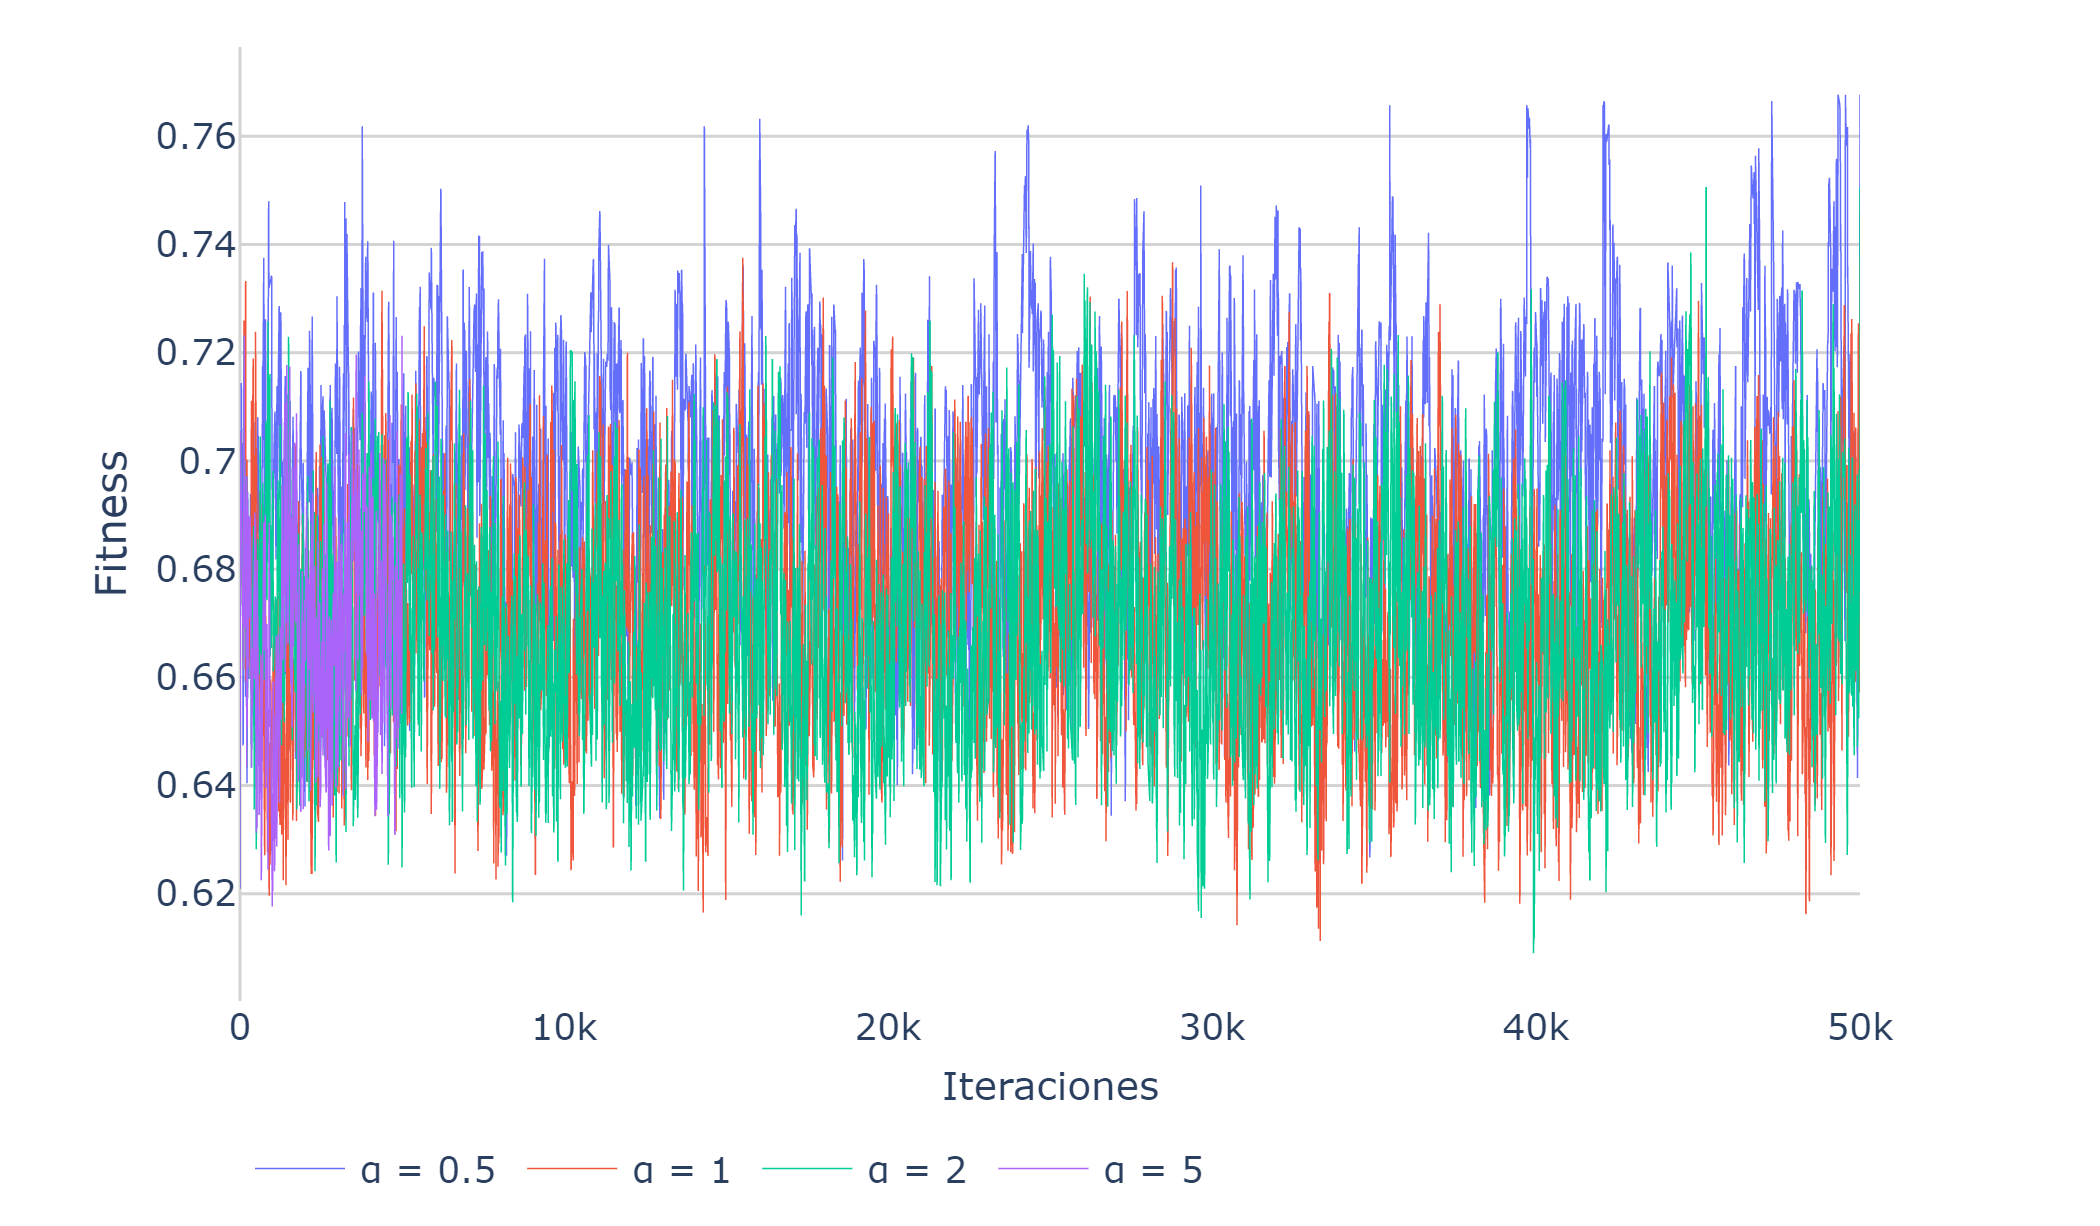
\includegraphics[width=\linewidth]{Caso3_comparativa-alphas_iteracion}
	\caption{Caso 3}
	\label{fig:Caso3_comparativa-alphas_iteracion}
	\centering
\end{subfigure}
	\caption{Evolución comparativa del desempeño del \textit{SVNS} con diferentes \textbf{$\alpha$} para el Caso 3 y el 9.}
\end{figure}

Las gráficas comparativas de los tipos de entornos, del tipo de VNS y de los distintos valores para el parámetro alpha incluidas en esta sección, junto con las demás del resto de los casos de prueba se encuentran disponibles y de manera interactiva en la web \url{https://sfv-tfm-recursos.000webhostapp.com/}.

\subsection{Comparación de metaheurísticas}
\label{sec:5:comparacion-metaheuristicas}

Una vez ajustados todos los parámetros para sacar el máximo rendimiento del sistema, podemos compararlo con otros, y en este caso, se ha hecho una comparación de resultados con la metaheurística \sa{} (SA), definida en la \autoref{sec:3:metaheurística}. Recuérdese que se trata de la metaheurística empleada para el desarrollo del sistema \legacy{} y que fue adaptada a las nuevas condiciones y restricciones del sistema implementado en este TFM.

Es importante destacar en este punto que la \faseuno{}, de inicialización, es la misma en ambas metaheurísticas. La única diferencia entre unas ejecuciones u otras está únicamente en la \fasedos{}, es decir, la metaheurística en sí.

Las Tablas \ref{table:comparativa-sa-vns-porcentaje} y \ref{table:comparativa-sa-vns-tiempo} recopilan los resultados medios (de 10 ejecuciones distintas) para ambas metaheurísticas, variando la condición de parada: porcentaje mínimo de mejora y tiempo máximo. El porcentaje de cada caso y de cada metaheurística empleados son aquellos con los que se alcanzan los resultados óptimos, por lo que dependen de las características tanto de las metaheurísticas como de los propios casos, por lo que no es invariante, a diferencia de la condición de parada por tiempo, que se optó por emplear un tiempo exacto de 10 minutos, de manera que forzamos a las metaheurísticas a ejecutar ese tiempo. 

Encontramos casos donde, tanto en VNS como en SA, empleando la condición de parada optimizada al porcentaje mínimo de mejora, terminaría su ejecución en un tiempo menor de los 10 minutos, pero también tenemos casos en los que sucede lo opuesto. Por ejemplo, el Caso 5 nos ocupa un tiempo de ejecución de 25 minutos, que al emplear como condición de parada el tiempo, se está limitando su tiempo de ejecución y por ende es natural que los resultados sean peores. Con la mayoría de los casos sucede lo contrario: tardan menos de los 10 minutos y, como vemos al comparar ambas tablas, en algunos casos hay una pequeña mejoría, pero no nos parece suficiente a cambio del tiempo empleado.

\begin{table}
	\centering
	\caption{Tabla comparativa con condición de parada establecida únicamente por porcentaje mínimo de mejora}
	\label{table:comparativa-sa-vns-porcentaje}
	\resizebox{\textwidth}{!}{%
		\begin{tabular}{cccccccccc}
			\hline
			\multicolumn{10}{c}{}                                                                                                                                                                                                                                                                                        \\
			\multicolumn{10}{c}{Condición de Parada: Porcentaje de mejora}                                                                                                                                                                                                                                               \\
			\multicolumn{10}{c}{}                                                                                                                                                                                                                                                                                        \\ \cline{3-10} 
			&     & \begin{tabular}[c]{@{}c@{}}Restricciones \\ incumplidas*\end{tabular} & \begin{tabular}[c]{@{}c@{}}Número de \\ controladores\end{tabular} & \begin{tabular}[c]{@{}c@{}}Fitness\\ total\end{tabular} & $f_1$    & $f_2$    & $f_3$    & $f_4$    & Tiempo (min) \\ \cline{3-10} 
			\multicolumn{10}{c}{}                                                                                                                                                                                                                                                                                        \\
			\multicolumn{1}{c|}{}                         & SA  & 58.13                                                                & {\color[HTML]{9A0000} \textbf{25}}                                 & {\color[HTML]{9A0000} \textbf{0.7117}}                  & 0.7229 & 0.8686 & 0.4400 & 0.5877 & 21.09        \\
			\multicolumn{1}{c|}{\multirow{-2}{*}{Caso 1}} & VNS & 12.8183                                                              & {\color[HTML]{9A0000} \textbf{24}}                                 & {\color[HTML]{9A0000} \textbf{0.9718}}                  & 1.0000 & 0.9703 & 1.0000 & 0.6632 & 6.1894       \\
			&     &                                                                      &                                                                    &                                                         &        &        &        &        &              \\
			\multicolumn{1}{c|}{}                         & SA  & -                                                                    & -                                                                  & -                                                       & -      & -      & -      & -      & -            \\
			\multicolumn{1}{c|}{\multirow{-2}{*}{Caso 3}} & VNS & 1.0778                                                              & 24                                                                 & 0.9662
			                                                  & 1.0000 & 0.9975 & 0.9167 & 0.6561  & 6.00       \\
			&     &                                                                      &                                                                    &                                                         &        &        &        &        &              \\
			\multicolumn{1}{c|}{}                         & SA  & 2.00                                                                 & 19                                                                 & 0.9111                                                  & 1.0000 & 0.9941 & 0.4737 & 0.8598 & 7.54         \\
			\multicolumn{1}{c|}{\multirow{-2}{*}{Caso 4}} & VNS & 2.00                                                               & 19                                                                 & 0.9105                                                  & 1.0000 & 0.9942 & 0.4737 & 0.8505 & 2.8527       \\
			&     &                                                                      &                                                                    &                                                         &        &        &        &        &              \\
			\multicolumn{1}{c|}{}                         & SA  & 0.00                                                                 & 20                                                                 & 0.9432                                                  & 1.0000 & 1.0000 & 0.8000 & 0.5539 & 4.76         \\
			\multicolumn{1}{c|}{\multirow{-2}{*}{Caso 5}} & VNS & 1.8000                                                               & 20                                                                 & 0.9668                                                  & 1.0000 & 0.9950 & 0.9000 & 0.7194 & 25.7926      \\
			&     &                                                                      &                                                                    &                                                         &        &        &        &        &              \\
			\multicolumn{1}{c|}{}                         & SA  & 5.00                                                                 & 19                                                                 & 0.9489                                                  & 1.0000 & 0.9795 & 0.7894 & 0.7675 & 9.68         \\
			\multicolumn{1}{c|}{\multirow{-2}{*}{Caso 6}} & VNS & 6.6200                                                               & 19                                                                 & 0.9467                                                  & 1.0000 & 0.9806 & 0.7895 & 0.7257 & 0.7935       \\
			&     &                                                                      &                                                                    &                                                         &        &        &        &        &              \\
			\multicolumn{1}{c|}{}                         & SA  & 27.50                                                                & {\color[HTML]{9A0000} \textbf{28}}                                 & {\color[HTML]{9A0000} \textbf{0.6146}}                  & 0.5221 & 0.9491 & 0.3000 & 0.6972 & 61.6         \\
			\multicolumn{1}{c|}{\multirow{-2}{*}{Caso 7}} & VNS & 5.2000                                                               & {\color[HTML]{9A0000} \textbf{26}}                                 & {\color[HTML]{9A0000} \textbf{0.9335}}                  & 1.0000 & 0.9889 & 0.6923 & 0.7102 & 7.5845       \\
			&     &                                                                      &                                                                    &                                                         &        &        &        &        &              \\
			\multicolumn{1}{c|}{}                         & SA  & 2.00                                                                 & 22                                                                 & 0.9684                                                  & 1.0000 & 0.9949 & 0.9090 & 0.7238 & 10.31        \\
			\multicolumn{1}{c|}{\multirow{-2}{*}{Caso 8}} & VNS & 4.4000                                                               & 22                                                                 & 0.9651                                                  & 1.0000 & 0.9889 & 0.9091 & 0.6953 & 22.5359      \\
			&     &                                                                      &                                                                    &                                                         &        &        &        &        &              \\
			\multicolumn{1}{c|}{}                         & SA  & 0.00                                                                 & 23                                                                 & 0.9711                                                  & 1.0000 & 1.0000 & 0.9130 & 0.7360 & 6.01         \\
			\multicolumn{1}{c|}{\multirow{-2}{*}{Caso 9}} & VNS & 4.0400                                                               & 23                                                                 & 0.9659                                                  & 1.0000 & 0.9902 & 0.9130 & 0.6923 & 9.3945       \\
			&     &                                                                      &                                                                    &                                                         &        &        &        &        &              \\
			\multicolumn{10}{c}{}                                                                                                                                                                                                                                                                                        \\ \hline
		\end{tabular}%
	}
	\footnotesize{*Valor de las restricciones ponderado}
\end{table}


\begin{table}
	\centering
	\caption{Tabla comparativa con condición de parada establecida que limita el tiempo de ejecución a 10 minutos}
	\label{table:comparativa-sa-vns-tiempo}
	\resizebox{\textwidth}{!}{%
		\begin{tabular}{cccccccccc}
			\hline
			\multicolumn{10}{c}{}                                                                                                                                                                                                                                                                                        \\
			\multicolumn{10}{c}{Condición de Parada: Tiempo de ejecución}                                                                                                                                                                                                                                                \\
			\multicolumn{10}{c}{}                                                                                                                                                                                                                                                                                        \\ \cline{3-10} 
			&     & \begin{tabular}[c]{@{}c@{}}Restricciones \\ incumplidas*\end{tabular} & \begin{tabular}[c]{@{}c@{}}Número de \\ controladores\end{tabular} & \begin{tabular}[c]{@{}c@{}}Fitness\\ total\end{tabular} & $f_1$  & $f_2$  & $f_3$  & $f_4$  & Tiempo (min) \\ \cline{3-10} 
			\multicolumn{10}{c}{}                                                                                                                                                                                                                                                                                        \\
			\multicolumn{1}{c|}{}                         & SA  & 6.00                                                                 & {\color[HTML]{9A0000} \textbf{27}}                                 & {\color[HTML]{9A0000} \textbf{0.6095}}                  & 0.4944 & 0.9877 & 0.3333 & 0.5946 & 10           \\
			\multicolumn{1}{c|}{\multirow{-2}{*}{Caso 1}} & VNS & 11.7111                                                              & {\color[HTML]{9A0000} \textbf{24}}                                 & {\color[HTML]{9A0000} \textbf{0.9721}}                  & 1.0000 & 0.9729 & 1.0000 & 0.6575 & 10           \\
			&     &                                                                      &                                                                    &                                                         &        &        &        &        &              \\
			\multicolumn{1}{c|}{}                         & SA  & -                                                                    & -                                                                  & -                                                       & -      & -      & -      & -      & -            \\
			\multicolumn{1}{c|}{\multirow{-2}{*}{Caso 3}} & VNS & 2.7944                                                              & 24                                                                 & 0.9656                                                  & 1.0000 & 0.9935 & 0.9167 & 0.6644 & 10           \\
			&     &                                                                      &                                                                    &                                                         &        &        &        &        &              \\
			\multicolumn{1}{c|}{}                         & SA  & 2.00                                                                 & 19                                                                 & 0.9107                                                  & 1.0000 & 0.9941 & 0.4737 & 0.8532 & 10           \\
			\multicolumn{1}{c|}{\multirow{-2}{*}{Caso 4}} & VNS & 2.00                                                               & 19                                                                 & 0.9107                                                  & 1.0000 & 0.9942 & 0.4737 & 0.8532 & 10           \\
			&     &                                                                      &                                                                    &                                                         &        &        &        &        &              \\
			\multicolumn{1}{c|}{}                         & SA  & 0.00                                                                 & 20                                                                 & 0.9599                                                  & 1.0000 & 1.0000 & 0.9000 & 0.5825 & 10           \\
			\multicolumn{1}{c|}{\multirow{-2}{*}{Caso 5}} & VNS & 1.75                                                               & 20                                                                 & 0.9659                                                  & 1.0000 & 0.9951 & 0.9000 & 0.7033 & 10           \\
			&     &                                                                      &                                                                    &                                                         &        &        &        &        &              \\
			\multicolumn{1}{c|}{}                         & SA  & 4.00                                                                 & 19                                                                 & 0.9483                                                  & 1.0000 & 0.9854 & 0.7895 & 0.7300 & 10           \\
			\multicolumn{1}{c|}{\multirow{-2}{*}{Caso 6}} & VNS & 9.35                                                               & 19                                                                 & 0.9436                                                  & 1.0000 & 0.9727 & 0.7895 & 0.7086 & 10           \\
			&     &                                                                      &                                                                    &                                                         &        &        &        &        &              \\
			\multicolumn{1}{c|}{}                         & SA  & 27.50                                                                & {\color[HTML]{9A0000} \textbf{28}}                                 & {\color[HTML]{9A0000} \textbf{0.6146}}                  & 0.5221 & 0.9491 & 0.3000 & 0.6972 & 10           \\
			\multicolumn{1}{c|}{\multirow{-2}{*}{Caso 7}} & VNS & 4.8101                                                               & {\color[HTML]{9A0000} \textbf{26}}                                 & {\color[HTML]{9A0000} \textbf{0.9337}}                  & 1.0000 & 0.9897 & 0.6923 & 0.7098 & 10           \\
			&     &                                                                      &                                                                    &                                                         &        &        &        &        &              \\
			\multicolumn{1}{c|}{}                         & SA  & 3.00                                                                 & 22                                                                 & 0.9702                                                  & 1.0000 & 0.9924 & 0.9000 & 0.7644 & 10           \\
			\multicolumn{1}{c|}{\multirow{-2}{*}{Caso 8}} & VNS & 4.75                                                               & 22                                                                 & 0.9642                                                  & 1.0000 & 0.9880 & 0.9091 & 0.6845 & 10           \\
			&     &                                                                      &                                                                    &                                                         &        &        &        &        &              \\
			\multicolumn{1}{c|}{}                         & SA  & 3.00                                                                 & 23                                                                 & 0.9689                                                  & 1.0000 & 0.9928 & 0.9130 & 0.7312 & 10           \\
			\multicolumn{1}{c|}{\multirow{-2}{*}{Caso 9}} & VNS & 5.0250                                                               & 23                                                                 & 0.9645                                                  & 1.0000 & 0.9879 & 0.9130 & 0.6798 & 10           \\
			&     &                                                                      &                                                                    &                                                         &        &        &        &        &              \\
			\multicolumn{10}{c}{}                                                                                                                                                                                                                                                                                        \\ \hline
		\end{tabular}%
	}
	\footnotesize{*Valor de las restricciones ponderado}
\end{table}

Por otra parte, lo más significativo que observamos se encuentra en los Casos 1 y 7, marcados en sendas tablas en negrita color rojo. En los que nuestra metaheurística, el VNS es claramente superior en relación al primer fitness, \ref{O1}, que recordemos, es el más relevante de todos, con mayor ponderación. Este valor está relacionado con aquel situado a su izquierda: el número de controladores que emplea la solución final. 

A continuación, analizaremos y mostraremos las soluciones obtenidas en cada fase del sistema para todos los casos, comenzando por los dos mencionados anteriormente.

En general, el VNS proporciona mejores resultados, aunque muy similares a los del salvo en los Casos 1 y 7, que el VNS lo supera y salvo en el Caso 9, donde el SA logra mejores resultados para el objetivo \ref{O2}, relativo a las restricciones incumplidas.

\subsubsection{Análisis del Caso 1}

Para el Caso 1, inicialmente tenemos un total de 24 controladores, como se puede ver en la \autoref{fig:5:solucion-inicial-caso1}, que asciende a 27 tras la \faseuno{} de inicialización: para poder codificar las condiciones del caso, se necesitan 3 controladores adicionales, \textit{imaginarios}, pues se abren dos sectores y se cierra uno a partir del slot 36, de forma que el sector que se cierra \texttt{ADL} (de color azul en la figura) es afín al sector \texttt{ADG} (en color marrón), que se abre, por lo que su carga se asigna directamente a esos controladores, siguiendo la heurística de inicialización ya descrita en la \autoref{sec:3:inicializacion-soluciones}. El otro sector que se abre no tiene posibilidades de ser sustituido, por lo que se añaden 3 controladores siguiendo una plantilla $3\times1$.

La \autoref{fig:5:solucion-fase1-caso1} muestra el resultado de la manipulación de la planificación inicial llevada a cabo por la \faseuno{} y que será tomada como solución inicial de la \fasedos{}.

\begin{figure}
	\centering
	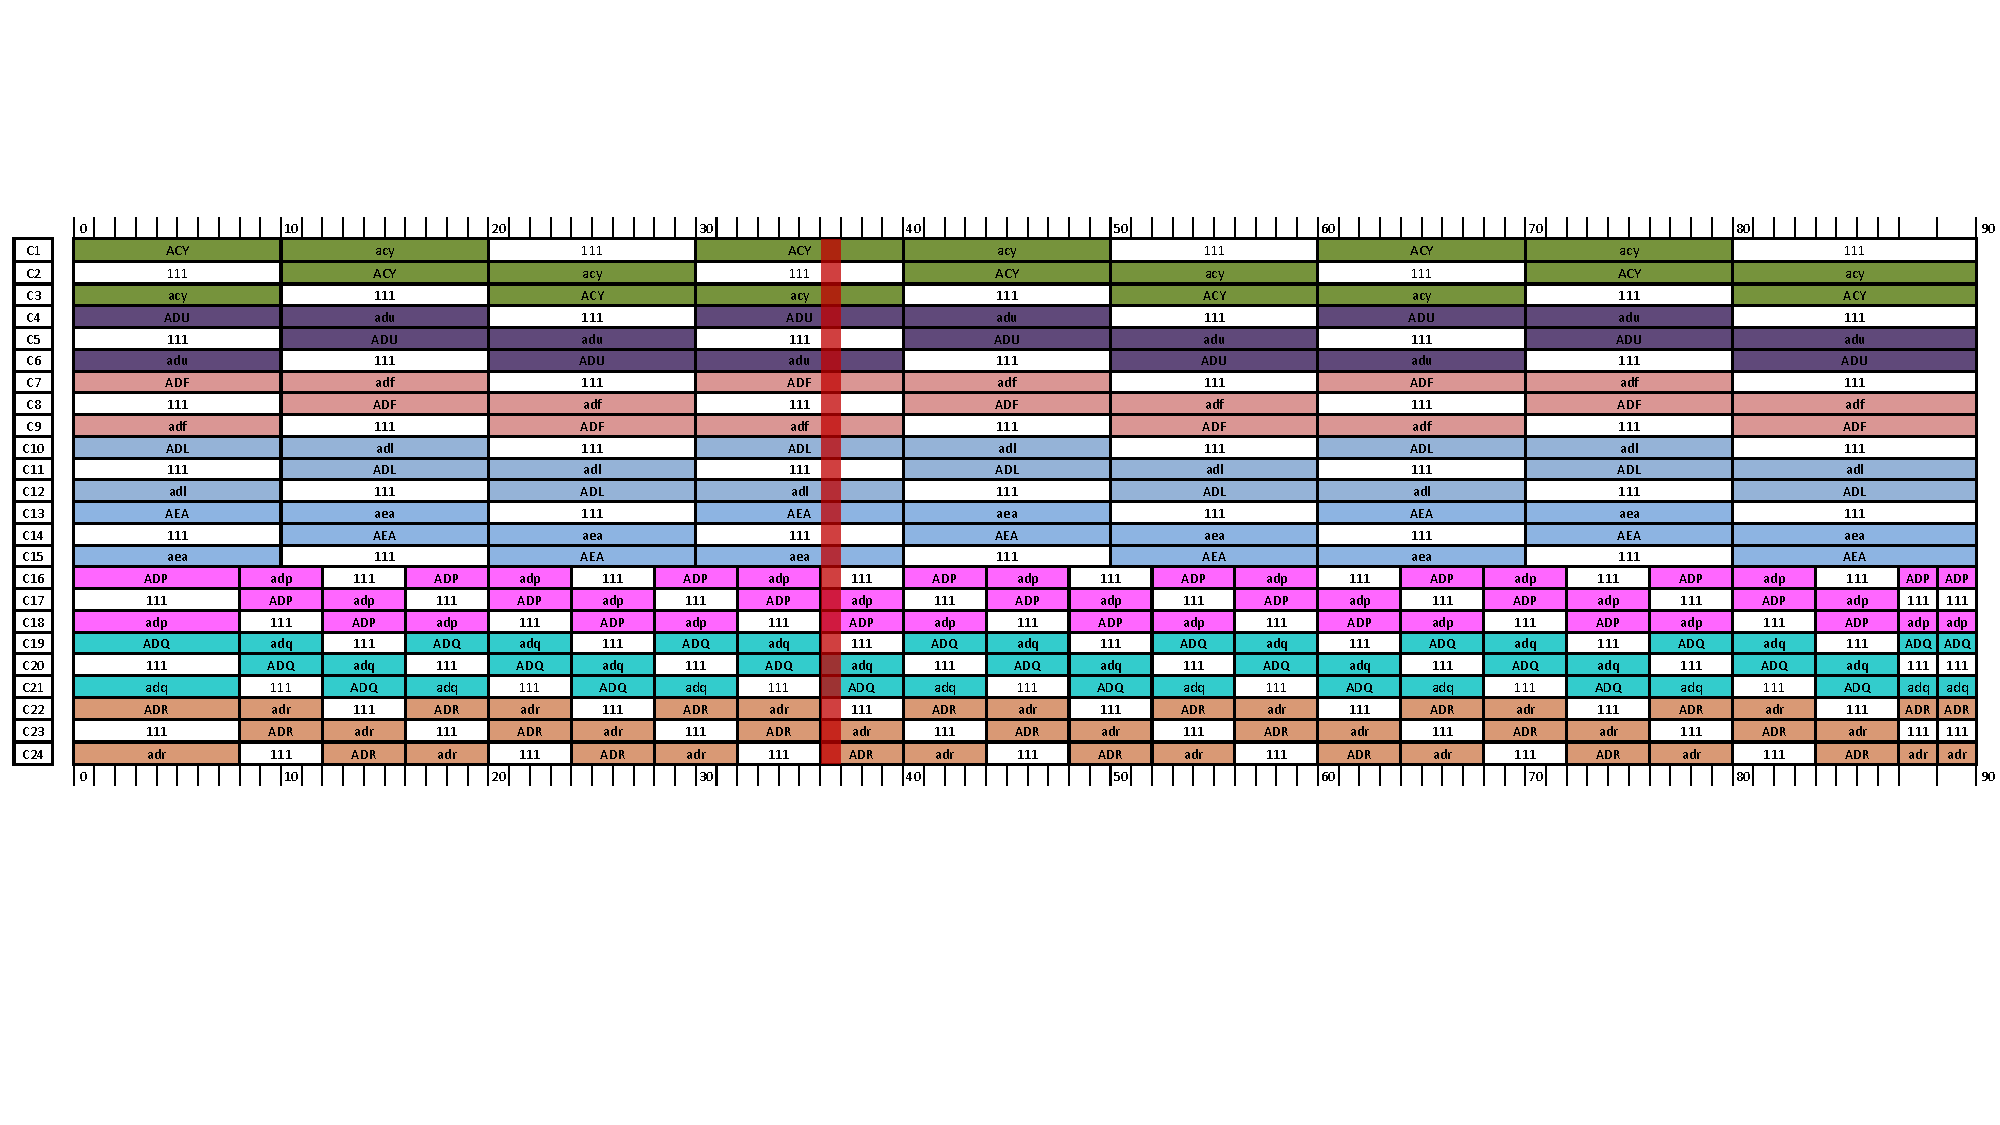
\includegraphics[width=\linewidth]{caso1/caso1-fase0}
	\caption{Planificación inicial del Caso 1.}
	\label{fig:5:solucion-inicial-caso1}
\end{figure}

\begin{figure}
	\centering
	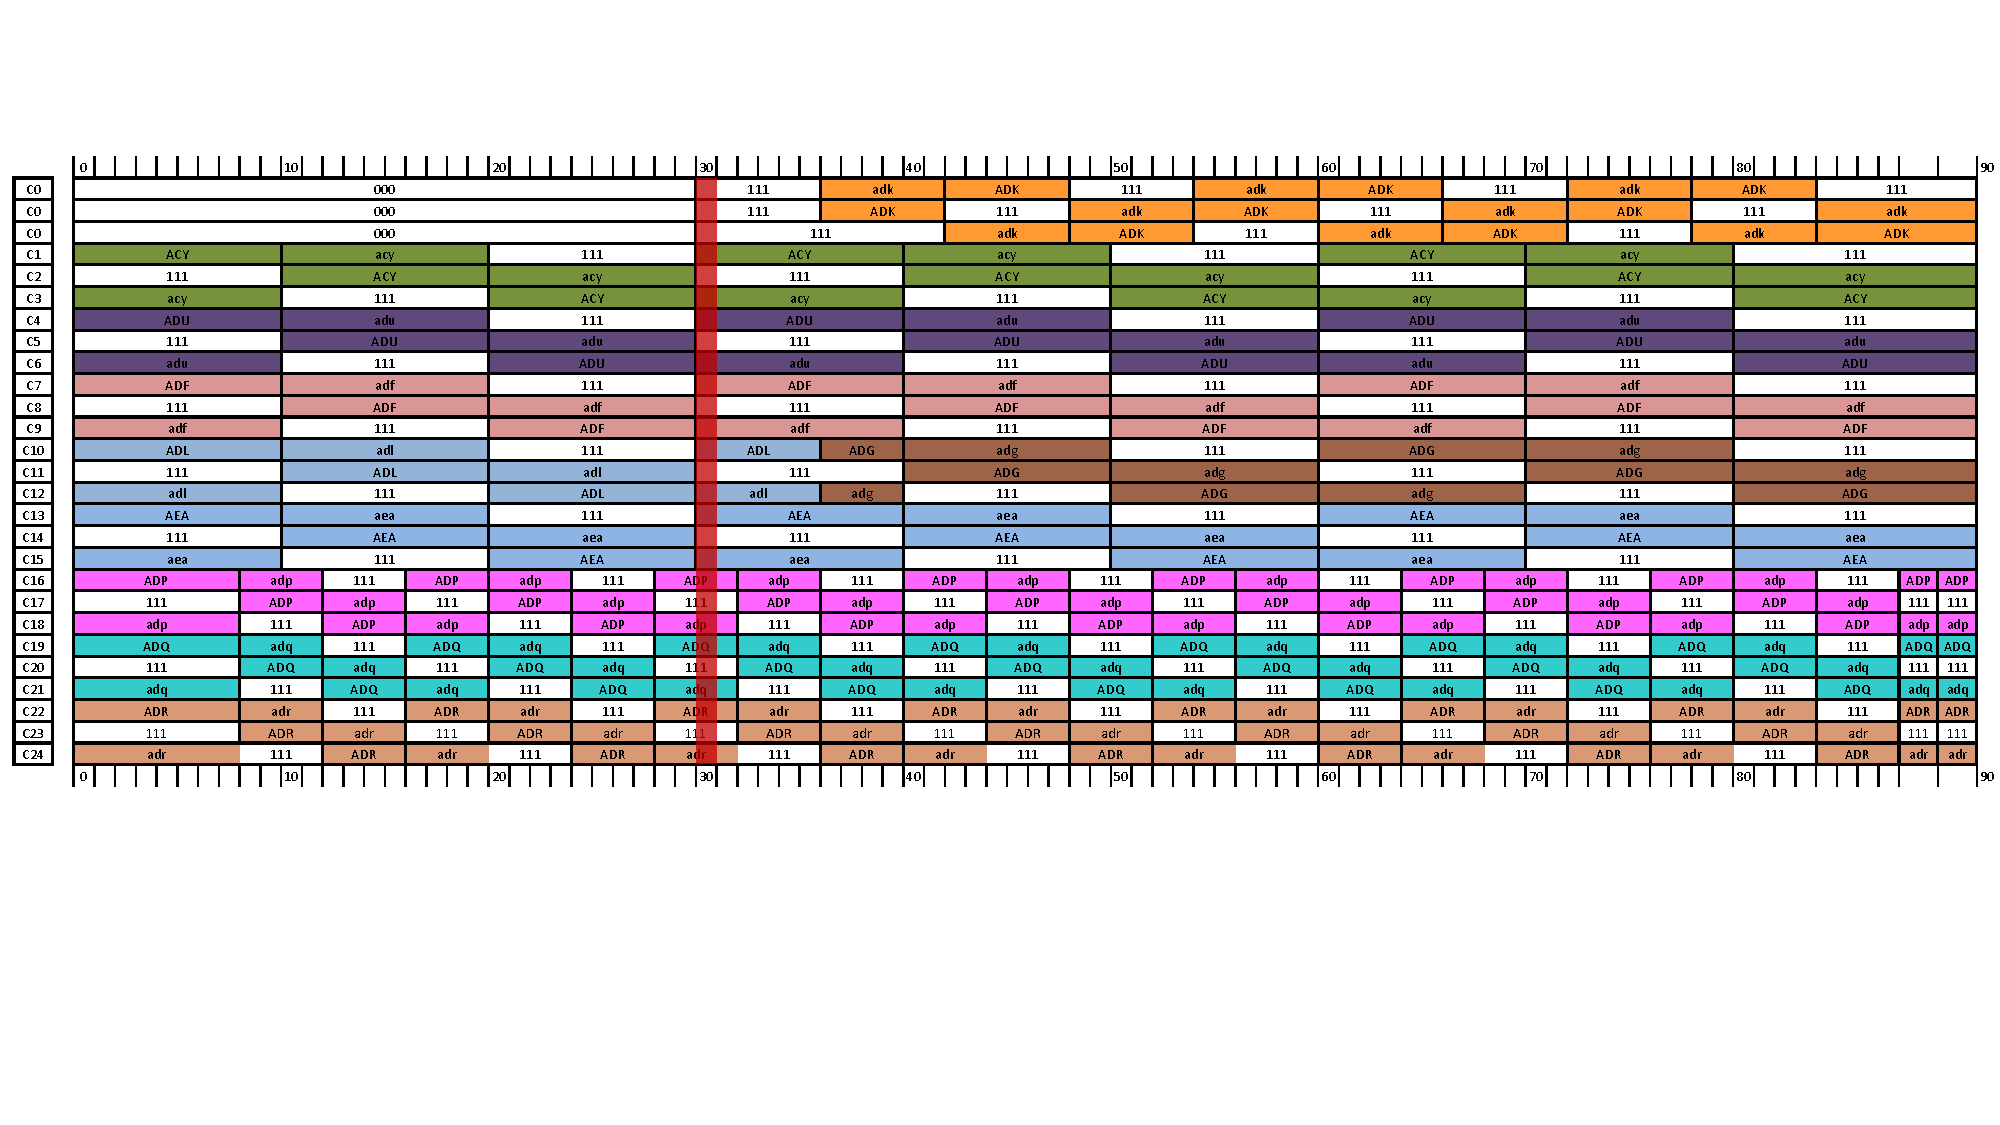
\includegraphics[width=\linewidth]{caso1/caso1-fase1}
	\caption{Solución inicial del Caso 1, obtenida como salida de la \faseuno{}.}
	\label{fig:5:solucion-fase1-caso1}
\end{figure}

Por su parte, la \fasedos{} que emplea la metaheurística de VNS (véase la \autoref{fig:5:solucion-fase2-vns-caso1}) logra eliminar todos los controladores imaginarios y reducir los recursos empleados a los mismos que los iniciales. Sin embargo, el SA (véase la \autoref{fig:5:solucion-fase2-sa-caso1}) no lo logra, dando como resultado una solución que emplea 25 controladores, uno más que la inicial. Como hemos mencionado, este valor es crítico para el sistema y por ello repercute en un gran impacto en el fitness, logrando el VNS un fitness total de $0.9718$ frente al $0.7117$ del SA. 

\begin{figure}
	\centering
	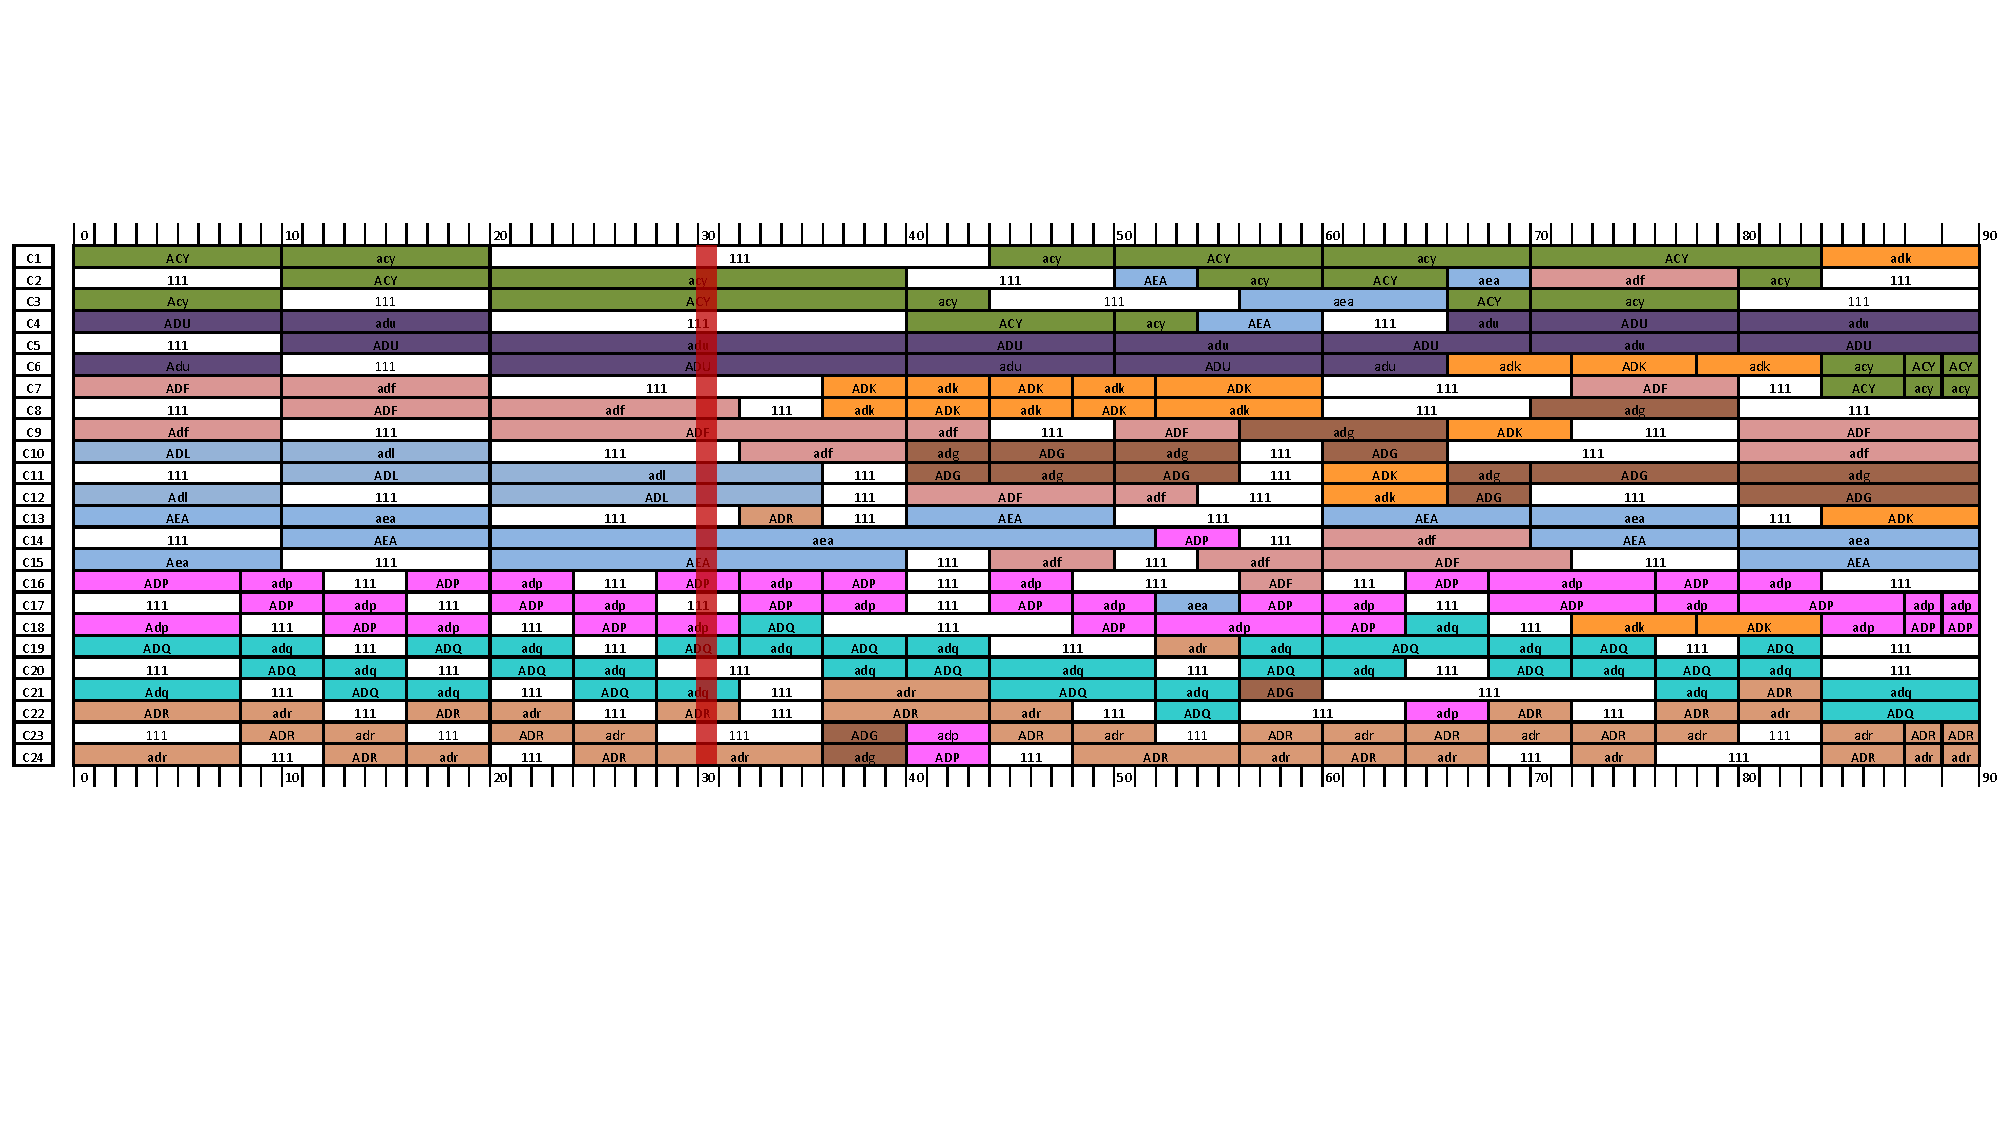
\includegraphics[width=\linewidth]{caso1/caso1-fase2-VNS}
	\caption{Solución final del sistema para el Caso 1, empleando para la \fasedos{} la metaheurística VNS.}
	\label{fig:5:solucion-fase2-vns-caso1}
\end{figure}

\begin{figure} 
	\centering
	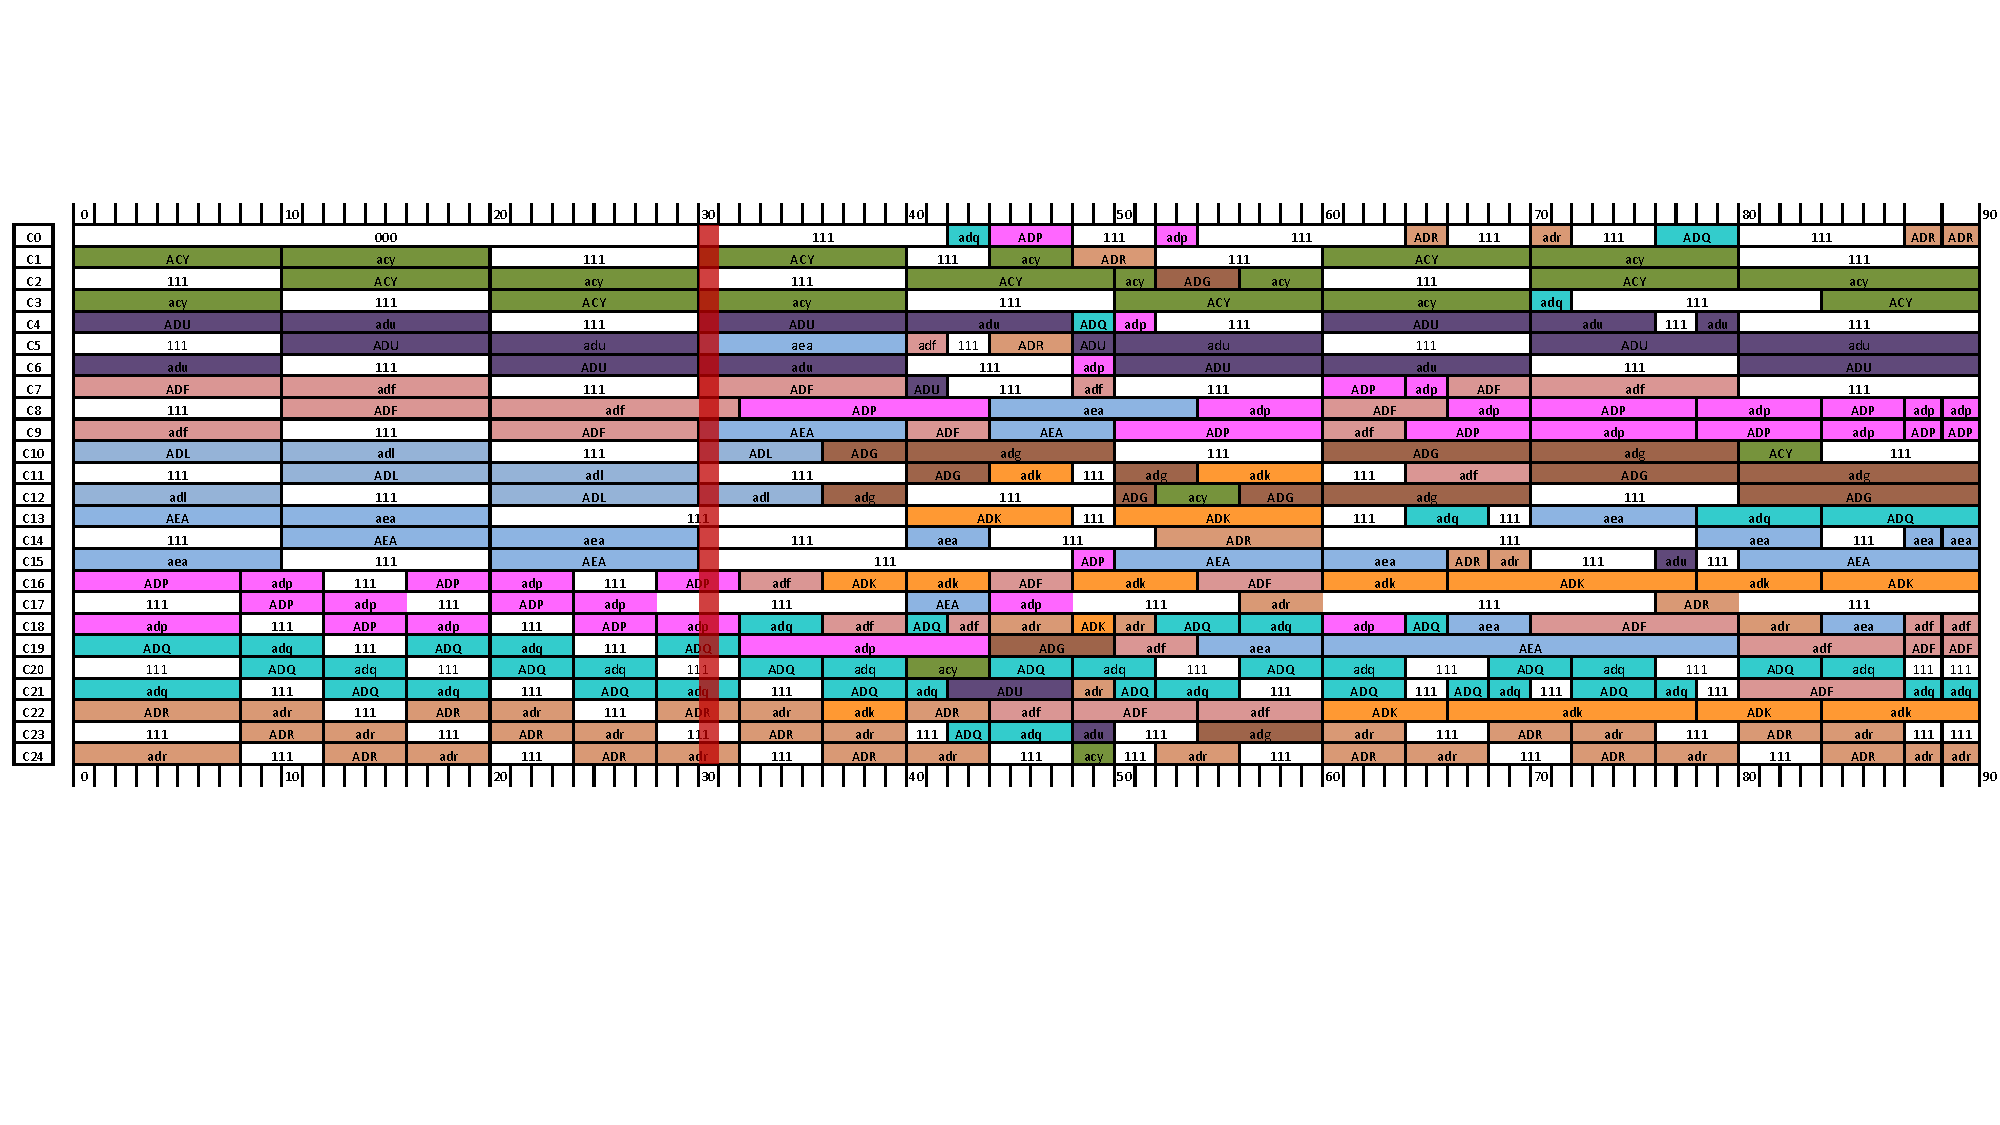
\includegraphics[width=\linewidth]{caso1/caso1-fase2-SA}
	\caption{Solución final del sistema para el Caso 1, empleando para la \fasedos{} la metaheurística SA.}
	\label{fig:5:solucion-fase2-sa-caso1}
\end{figure}

En cuanto a restricciones (\ref{O2}), la solución de VNS pasa inicialmente de incumplir 3 veces la restricción \ref{RD:9:tiempo-min-trabajo-continuado}, pues los dos últimos slots asignados a los controladores C16, C19 y C22 son de trabajo, lo que hace un total de 10 minutos, cuando el tiempo de trabajo mínimo es de 15 minutos, que son 3 slots.

Al adaptar la planificación inicial al problema del Caso 1, añadimos el incumplimiento de una restricción más: \ref{RD:controlador-por-cada-turno}, pues existen 3 turnos sin controlador real asignado.

Por último, la solución final logra reparar los problemas relativos a ambas restricciones antes nombradas, sin embargo a costa de incumplir las restricciones \ref{R:5:max-trabajo-continuado} y \ref{RD:3:porcentaje-min-descanso}, que están relacionadas entre sí, en 6 y 4 ocasiones respectivamente: para la solución que propone el sistema, algunos controladores deberán de trabajar más tiempo del adecuado y por consiguiente, descansar menos tiempo, algunos incluso por debajo del mínimo de tiempo total de la jornada.

Respecto al objetivo \ref{O3} y el objetivo \ref{O4}, el VNS parece que lo afronta mejor. Podemos apreciarlo visualmente: el momento del cambio es más homogéneo y la similitud a las plantillas es mayor en el caso del VNS.

\subsubsection{Análisis del Caso 7}

En el Caso 7 obtenemos unas soluciones peores que en otros casos, algo comprensible teniendo en cuenta la dificultad del mismo (véase la \autoref{sec:5:def-casos}), pero muy superiores pese a ello a las del SA. 

La planificación inicial de la que partimos consta de un total de 25 controladores. 
En la \faseuno{} se producen tres incidencias: varios cambios de sectorización, una baja y un alta.
La forma en la que las sectorizaciones cambian se encuentra representada en la \autoref{fig:5:esquema-sectorizacion-caso7}, que agrupa por colores aquellos sectores afines. 
Recuérdese que no es la misma sectorización 3A para el núcleo Ruta Este que para el Oeste. 

En la \autoref{fig:5:solucion-inicial-caso7} puede observarse el resultado del proceso que describiremos a continuación.

El núcleo Oeste pasa de una configuración 5A a una 5C a partir del slot 20, cerrándose cuatro sectores (ADL, ADP, ADQ y ADR) y abriéndose otros cuatro (ADH, ADI, ADM y ADN); uno de ellos permanece estático (AEA). 
A la hora de sustituir por afinidades (véase la \autoref{sec:3:fase1-paso1}), la heurística implementada sustituirá ADL por ADH, ADP por ADM y ADR por ADN, tal y como muestran ambas figuras. Por lo tanto, no es necesario añadir plantillas para estos sectores. 

Por último, al no haber afinidades entre los dos sectores que faltan, se ha de eliminar, durante el periodo de tiempo pertinente, la presencia del sector ADQ en la solución y añadir una nueva plantilla con tres controladores imaginarios para el sector ADI.

\begin{figure}
	\centering
	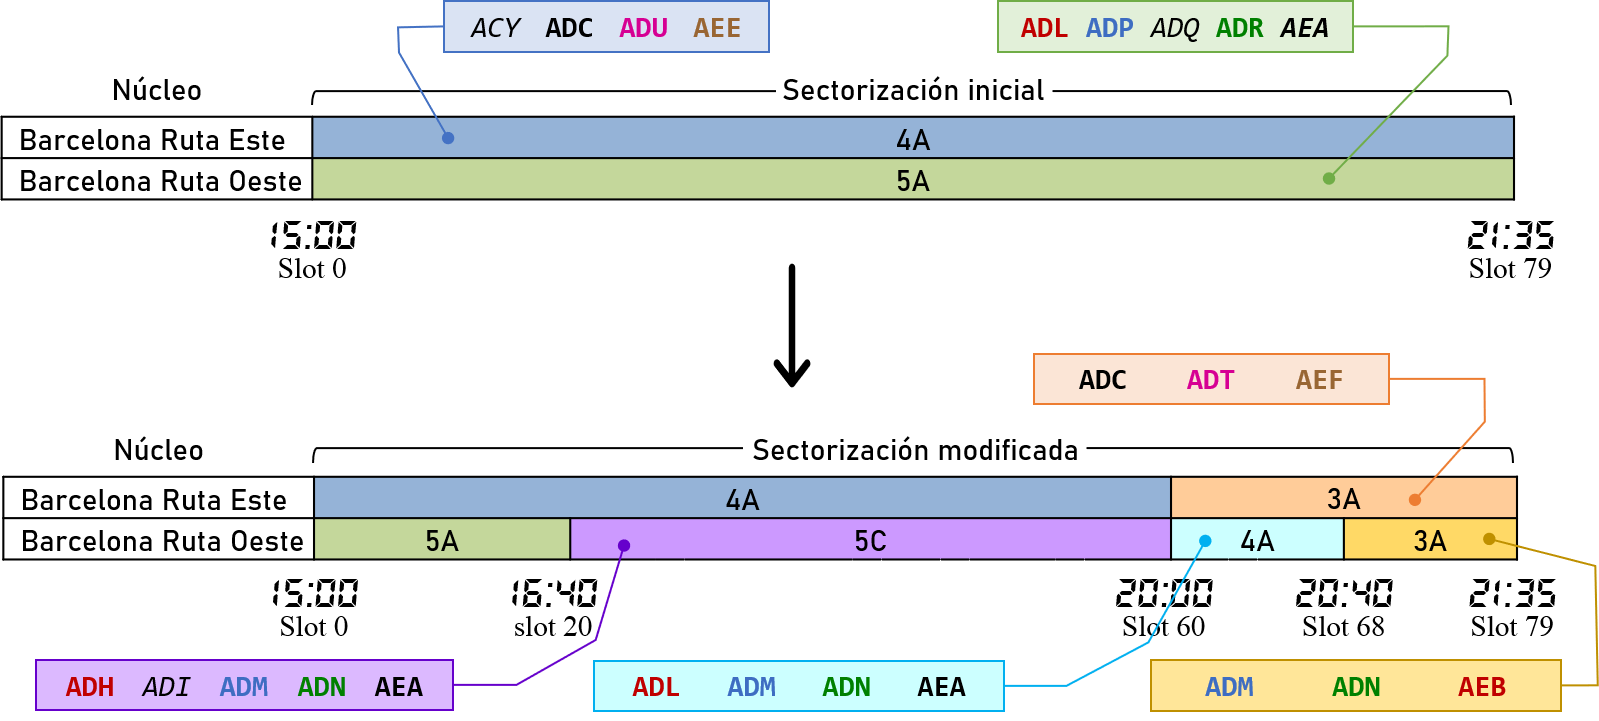
\includegraphics[width=\linewidth]{esquema-sectorizacion-caso7}
	\caption{Sectorización inicial y la modificada para el Caso 7.}
	\label{fig:5:esquema-sectorizacion-caso7}
\end{figure}

Por otro lado, para gestionar la baja del controlador C23 que se produce en el slot 42, se mueve toda su carga a partir de ese instante a un nuevo controlador imaginario, marcando ese intervalo de tiempo en C23 como inamovible para la \fasedos{} (mediante el ``000'').
Para gestionar el alta del nuevo controlador C26, se añade al final, y solo se permite que la \fasedos{} añada carga a partir del slot 60, que es cuando se produce el alta. De esta forma, la solución inicial que ofrece la \faseuno{} consta de un total de 28 controladores, de los cuales cuatro son imaginarios (véase la \autoref{fig:5:solucion-inicial-caso7}).

\begin{figure}
	\centering
	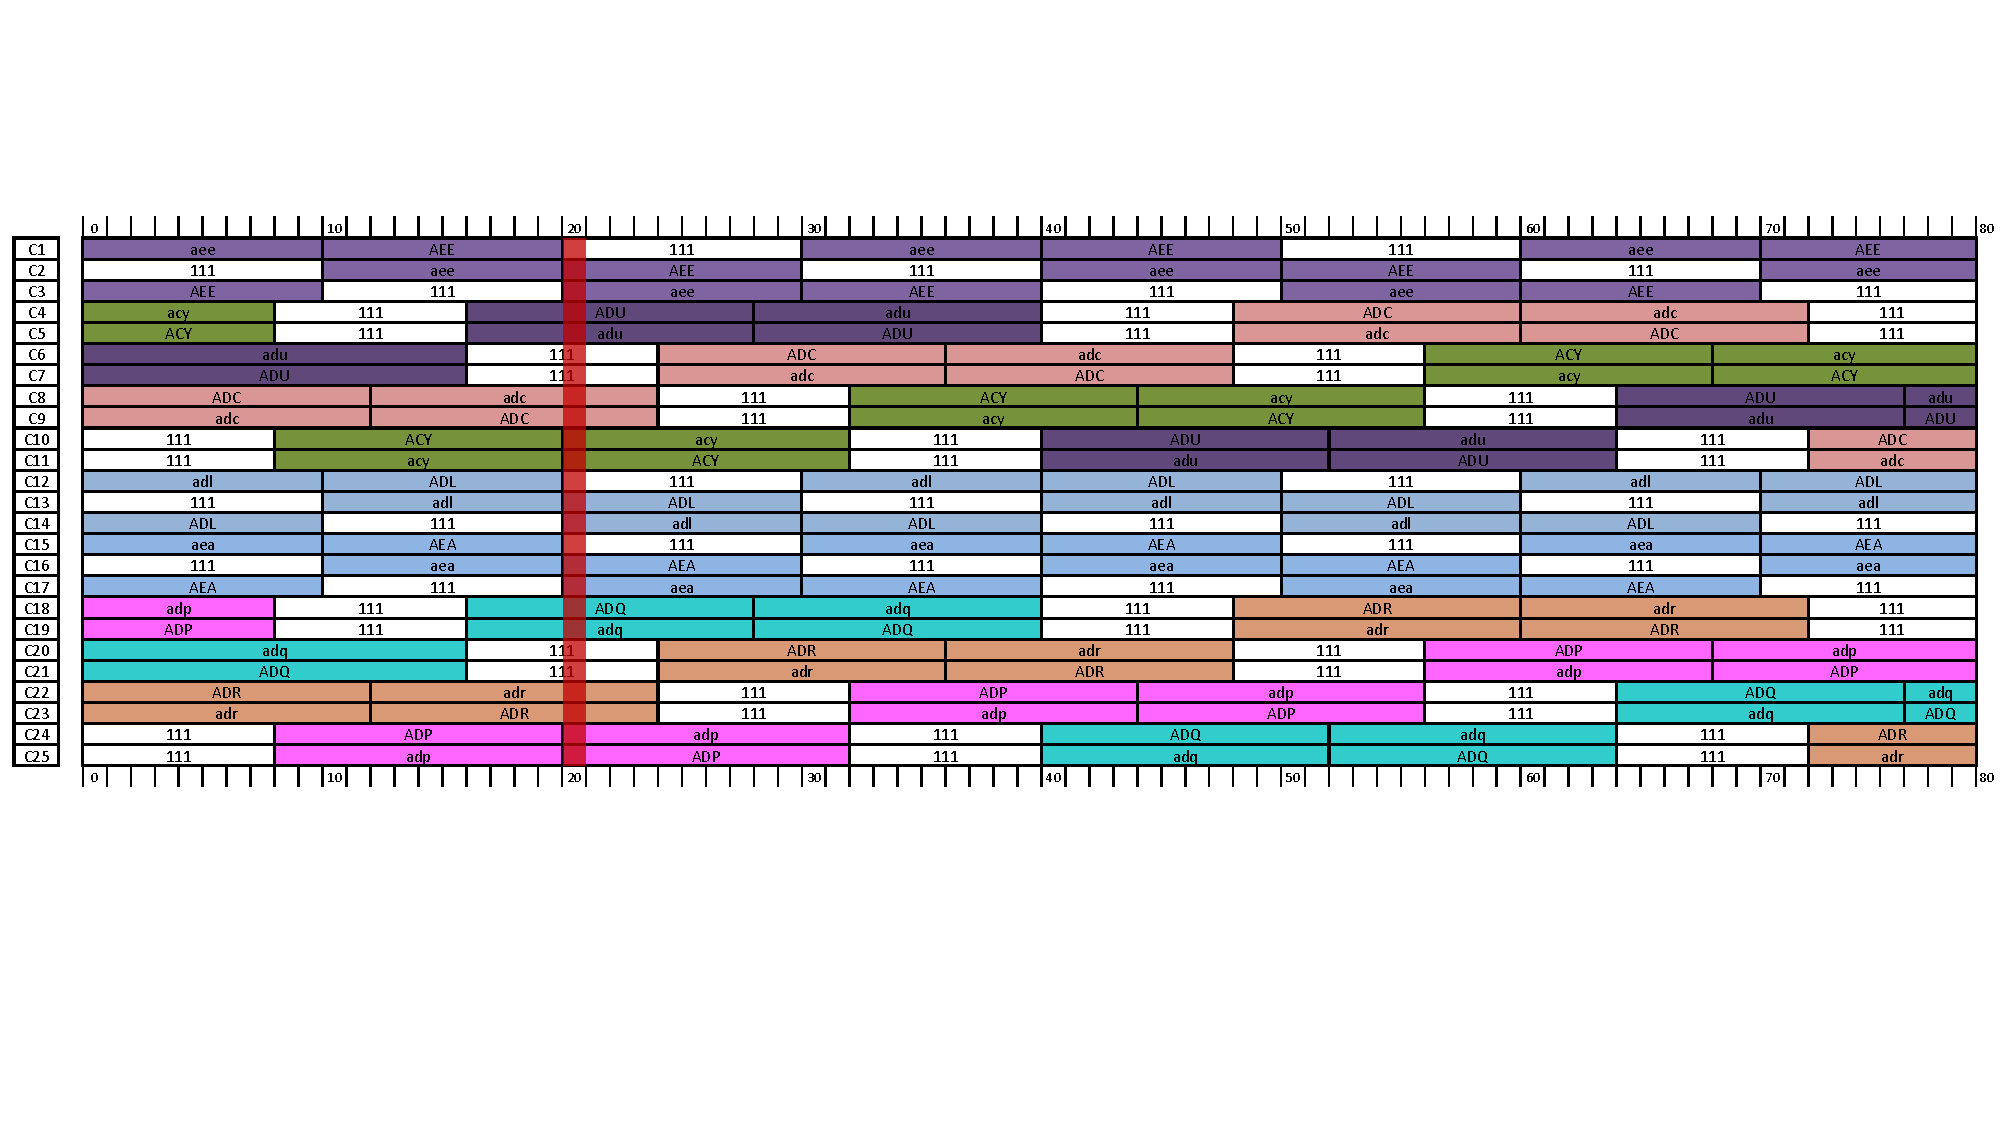
\includegraphics[width=\linewidth]{caso7/caso7-fase0}
	\caption{Planificación inicial del Caso 7.}
	\label{fig:5:solucion-inicial-caso7}
\end{figure}

\begin{figure}
	\centering
	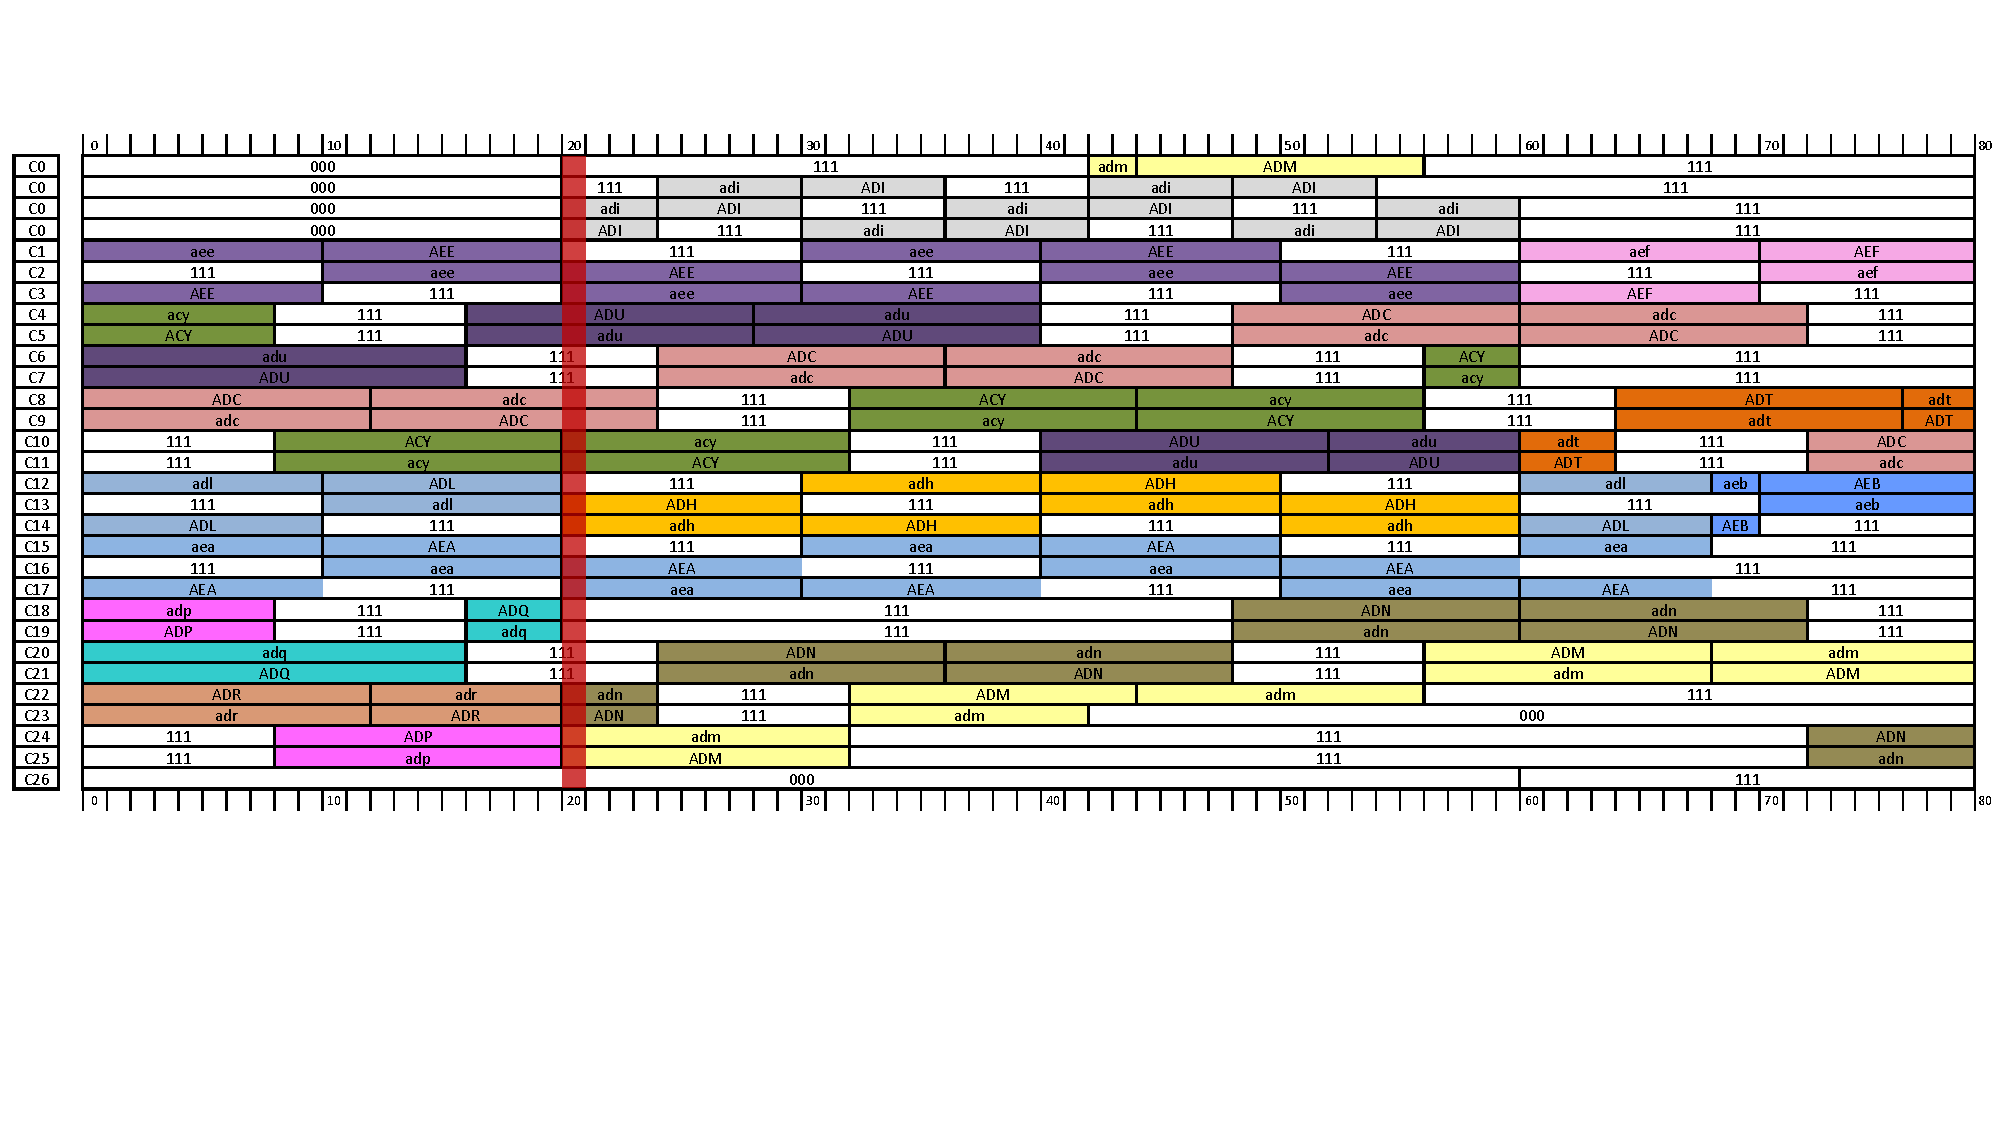
\includegraphics[width=\linewidth]{caso7/caso7-fase1}
	\caption{Solución inicial del Caso 7, obtenida como salida de la \faseuno{}.}
	\label{fig:5:solucion-fase1-caso7}
\end{figure}

La \fasedos{} toma dicha planificación y la logra reducir a 26 controladores en su solución final, eliminando todos los imaginarios (véase la \autoref{fig:5:solucion-fase2-vns-caso7}). Una diferencia muy grande respecto al SA, que ni siquiera logra reducir un solo controlador (véase la \autoref{fig:5:solucion-fase2-sa-caso7}). Por ello, la diferencia de valor total de la solución es muy grande: el SA obtiene una media de $0.6146$ mientras que el VNS logra la cifra de $0.9335$.

\begin{figure}
	\centering
	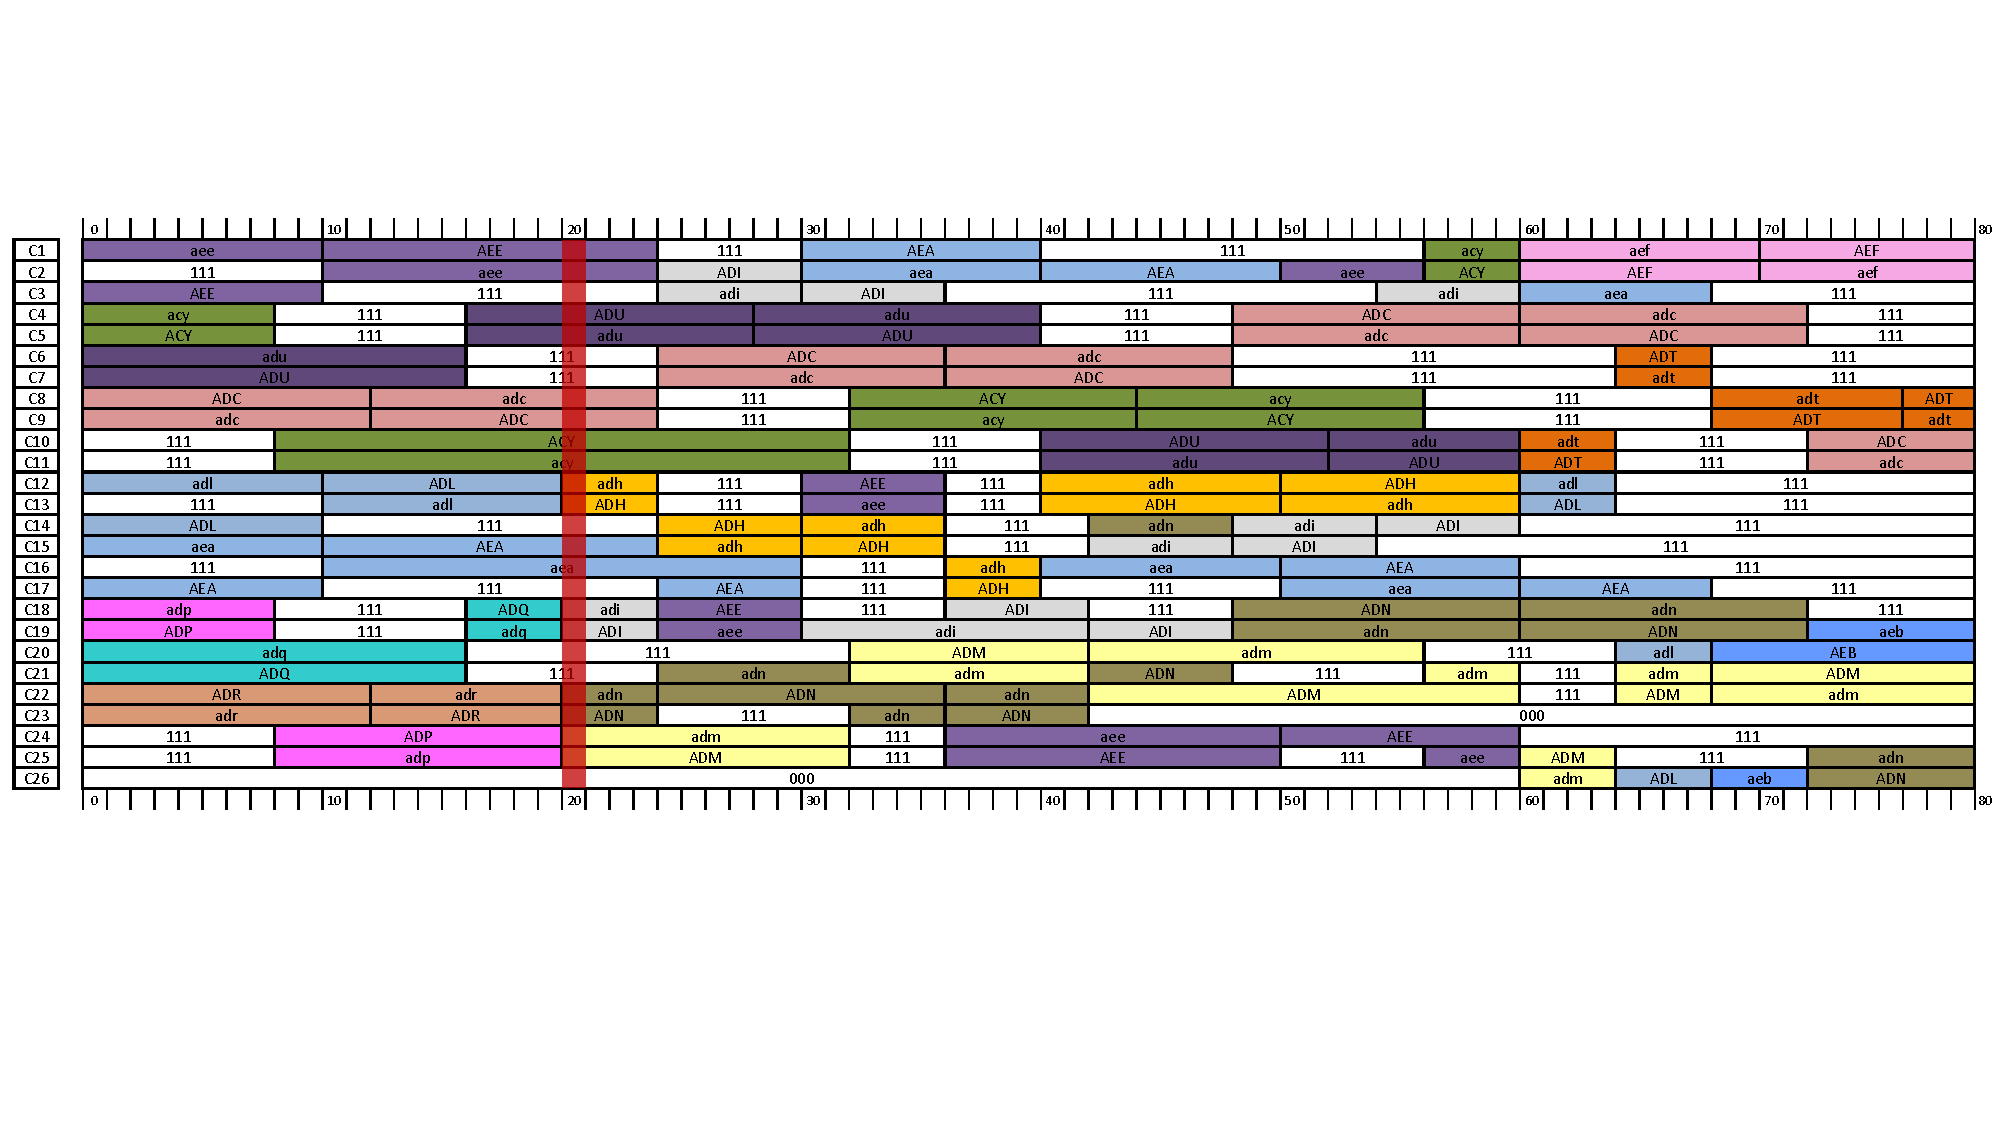
\includegraphics[width=\linewidth]{caso7/caso7-fase2-VNS}
	\caption{Solución final del sistema para el Caso 7, empleando para la \fasedos{} la metaheurística VNS.}
	\label{fig:5:solucion-fase2-vns-caso7}
\end{figure}

\begin{figure}
	\centering
	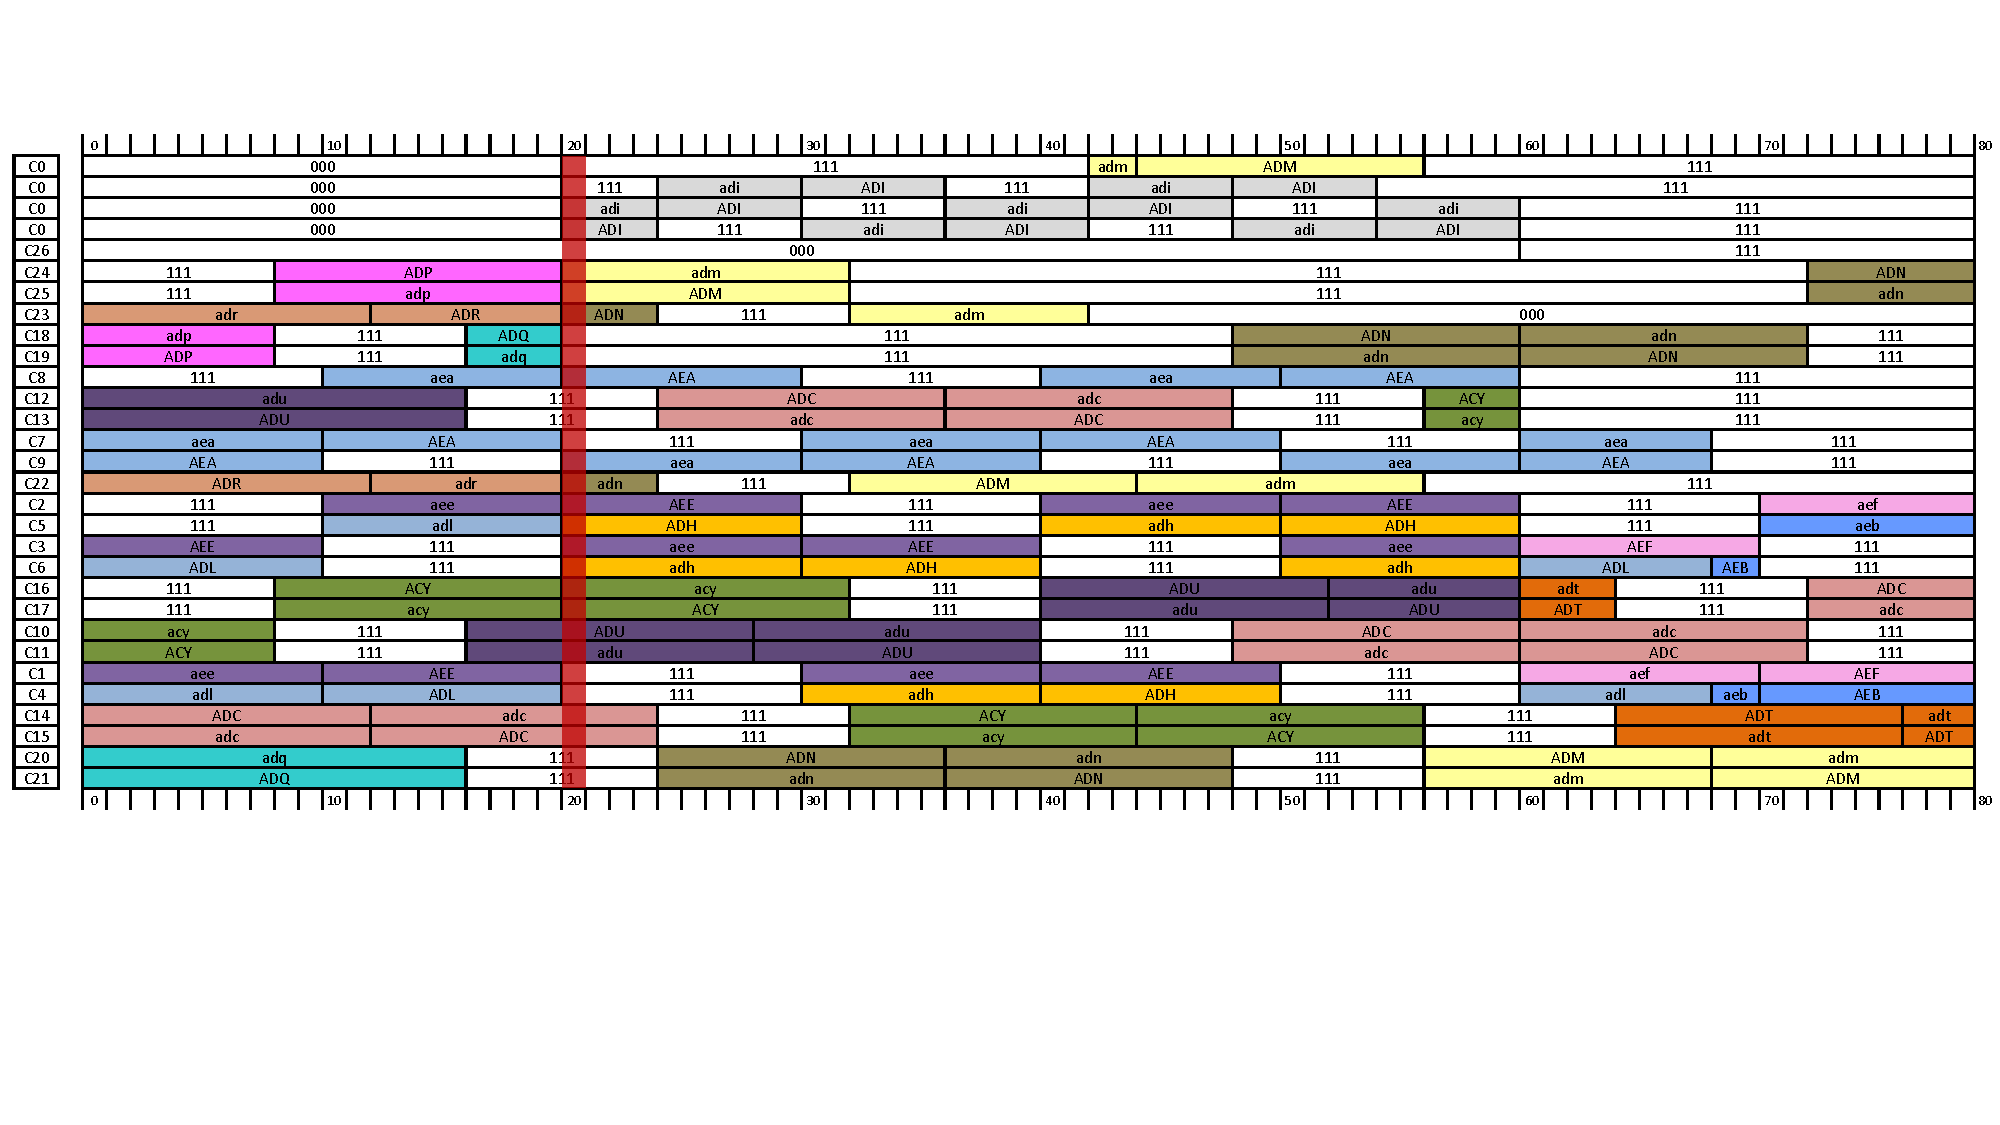
\includegraphics[width=\linewidth]{caso7/caso7-fase2-SA}
	\caption{Solución final del sistema para el Caso 7, empleando para la \fasedos{} la metaheurística SA.}
	\label{fig:5:solucion-fase2-sa-caso7}
\end{figure}

En cuanto a los demás objetivos, VNS es superior aunque similar tanto para el número de restricciones incumplidas \ref{O2} como para la semejanza a las plantillas \ref{O4}, aunque observamos resultados notablemente mejor, en media, para el \ref{O3}: la minimización del número de cambios en sala en el momento de la incidencia.

\subsubsection{Análisis del Caso 3}

Para este caso no disponemos de datos del SA, no obstante analizaremos los resultados obtenidos para el VNS.

Partimos de una planificación inicial idéntica a la anterior, con la única diferencia la hora del momento del cambio. De manera que partimos con un total de 24 controladores (\autoref{fig:caso3-fase0}) que, en este caso, debido a las necesidades de la incidencia, aumenta con un controlador imaginario adicional (véase la \autoref{fig:caso3-fase1}) al que se le pasa toda la carga del C23 a partir del slot 24, que es el que corresponde a la hora de la baja, las 9:30. Podemos observar cómo a partir de dicho slot, el controlador C23 tiene únicamente el valor de fuera de turno (``000'').

\begin{figure}
	\centering
	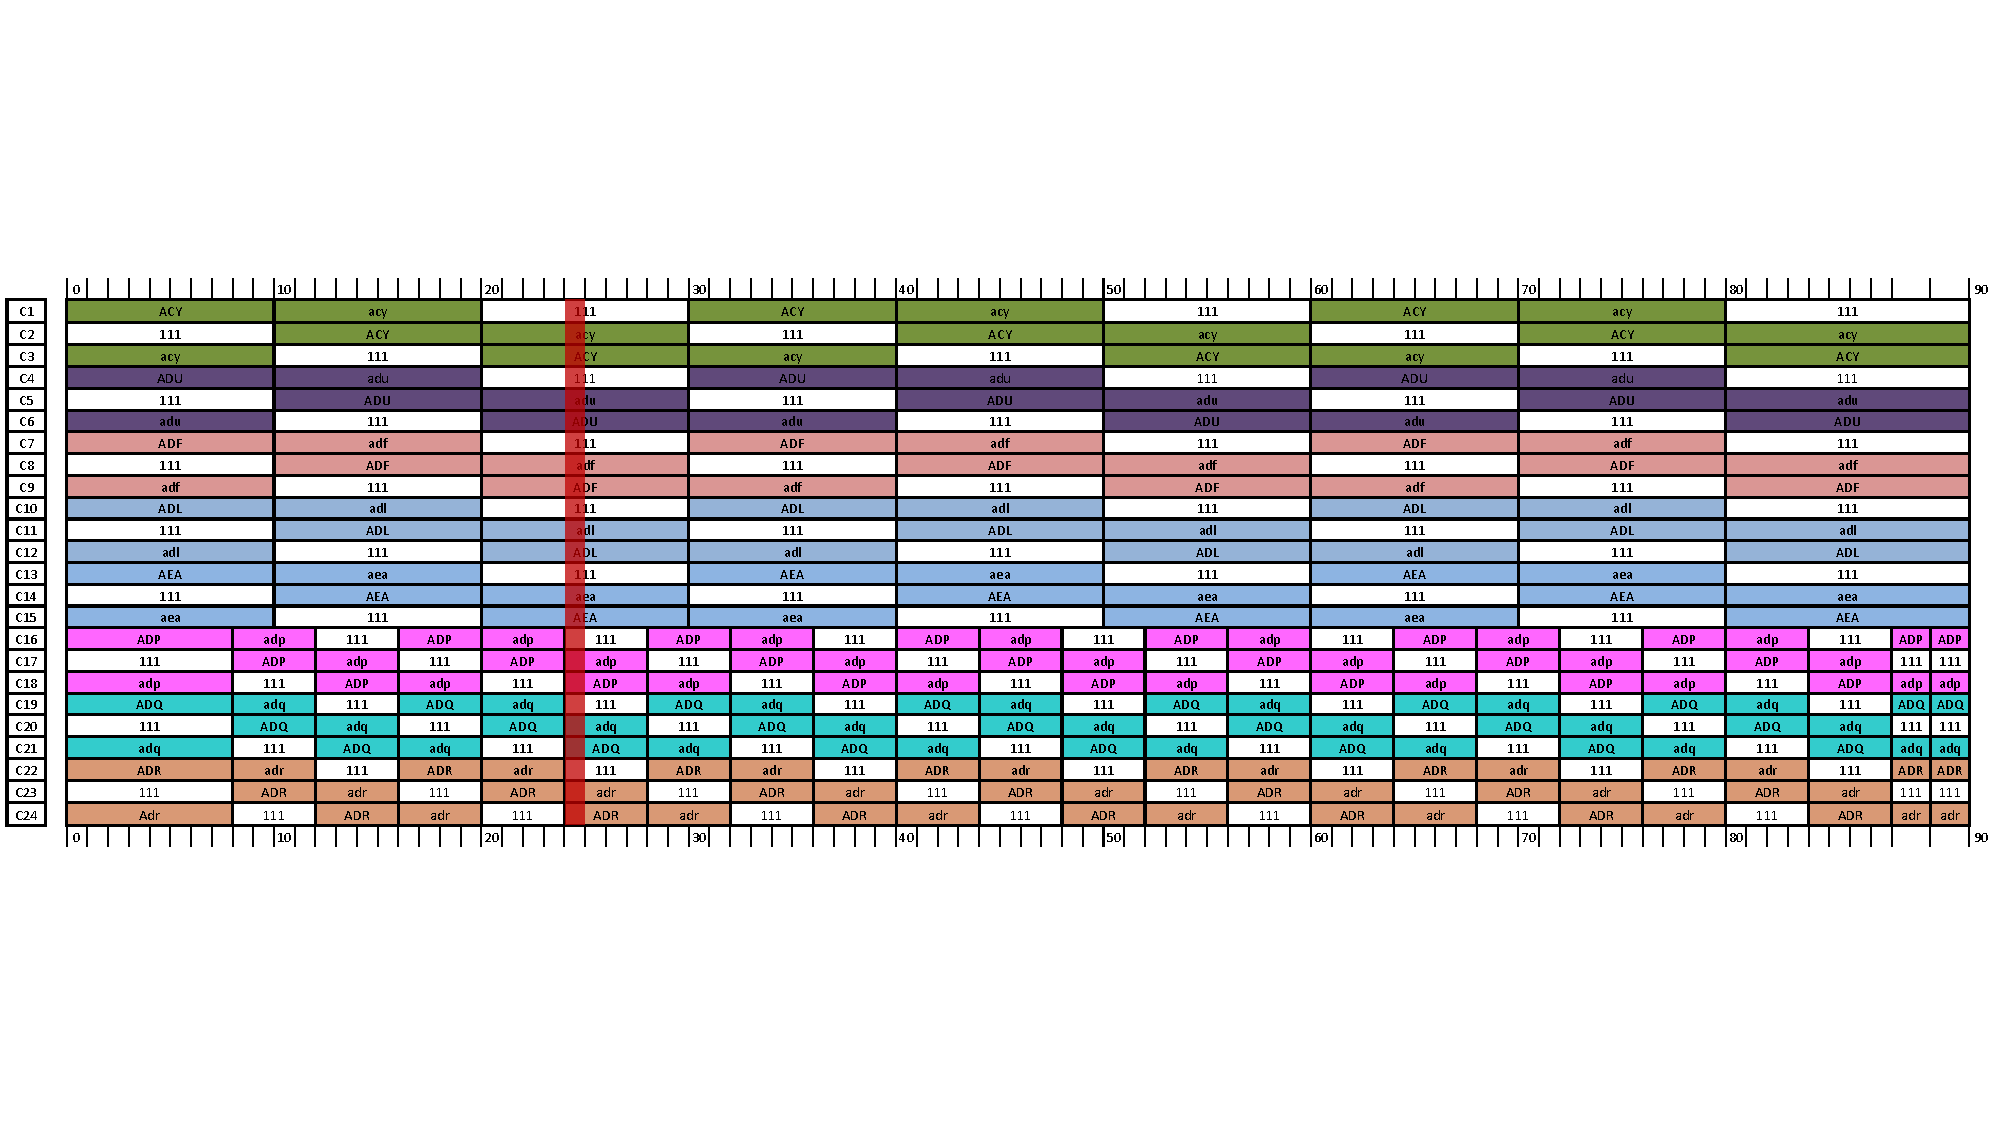
\includegraphics[width=\linewidth]{caso3/caso3-fase0}
	\caption{Planificación inicial del Caso 3}
	\label{fig:caso3-fase0}
\end{figure}

\begin{figure}
	\centering
	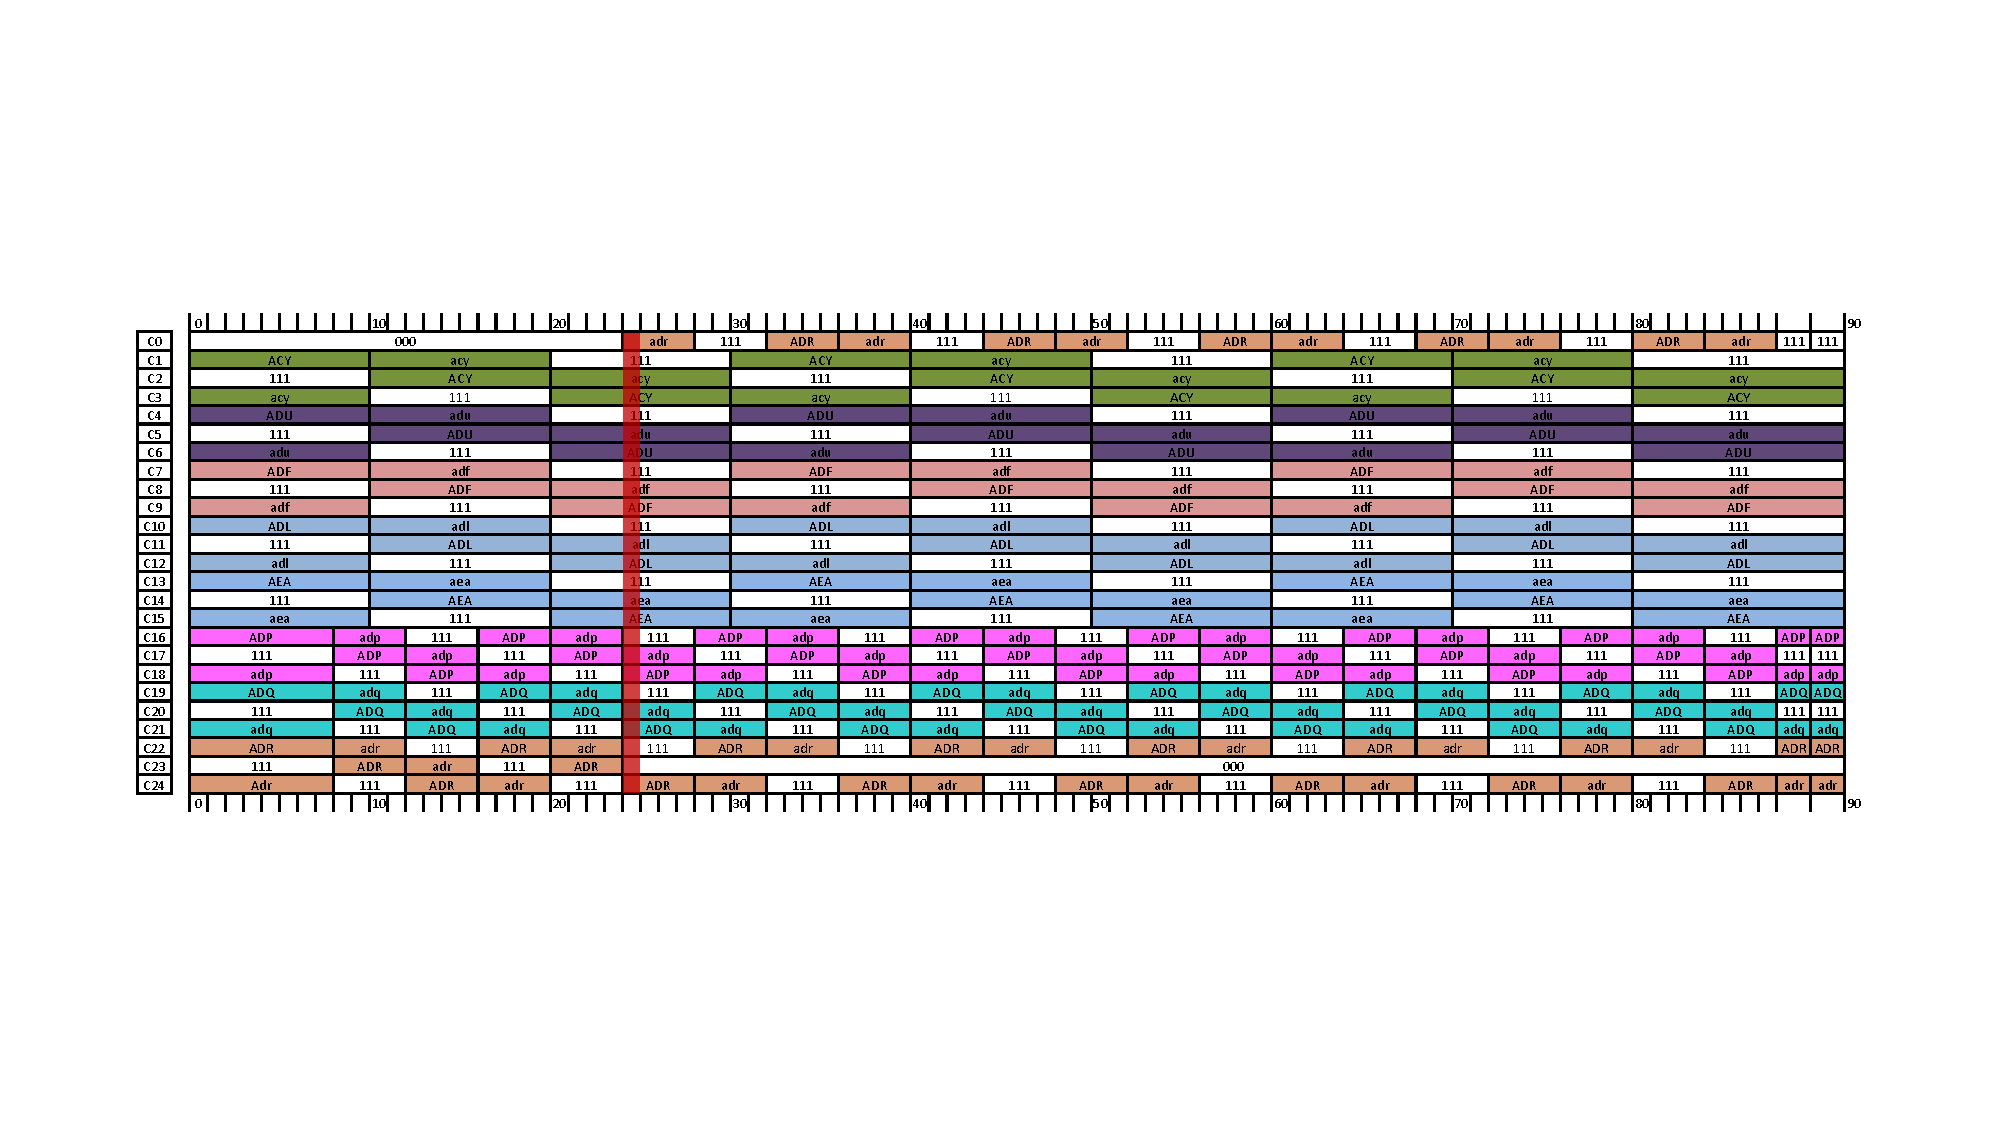
\includegraphics[width=\linewidth]{caso3/caso3-fase1}
	\caption{Solución inicial (\faseuno{}) para el Caso 3}
	\label{fig:caso3-fase1}
\end{figure}

La \fasedos{} no modifica este conjunto de slots, tal y como podemos observar en la solución final de la \autoref{fig:caso3-fase2}. De hecho, las modificaciones que observamos son mínimas para eliminar el imaginario. El objetivo \ref{O3}, relativo a los cambios de sala, ya parte de un valor óptimo. Lograr el objetivo primario, \ref{O1} se logra a expensas de destruir la estructura, es decir, el \ref{O4}. Esto es así porque es cómo lo hemos diseñado: es más importante el primer objetivo que el segundo y así sucesivamente. En cuanto al objetivo \ref{O2}, relativo a las restricciones, en la instancia concreta que presentamos en dicha figura, tiene un valor óptimo de 1, puesto que no se incumple ninguna. Y aunque en media no siempre sea así, dicha función objetivo se mueve entorno a un 0.99 en media, lo cual es un valor más que aceptable.

\begin{figure}[!h]
	\centering
	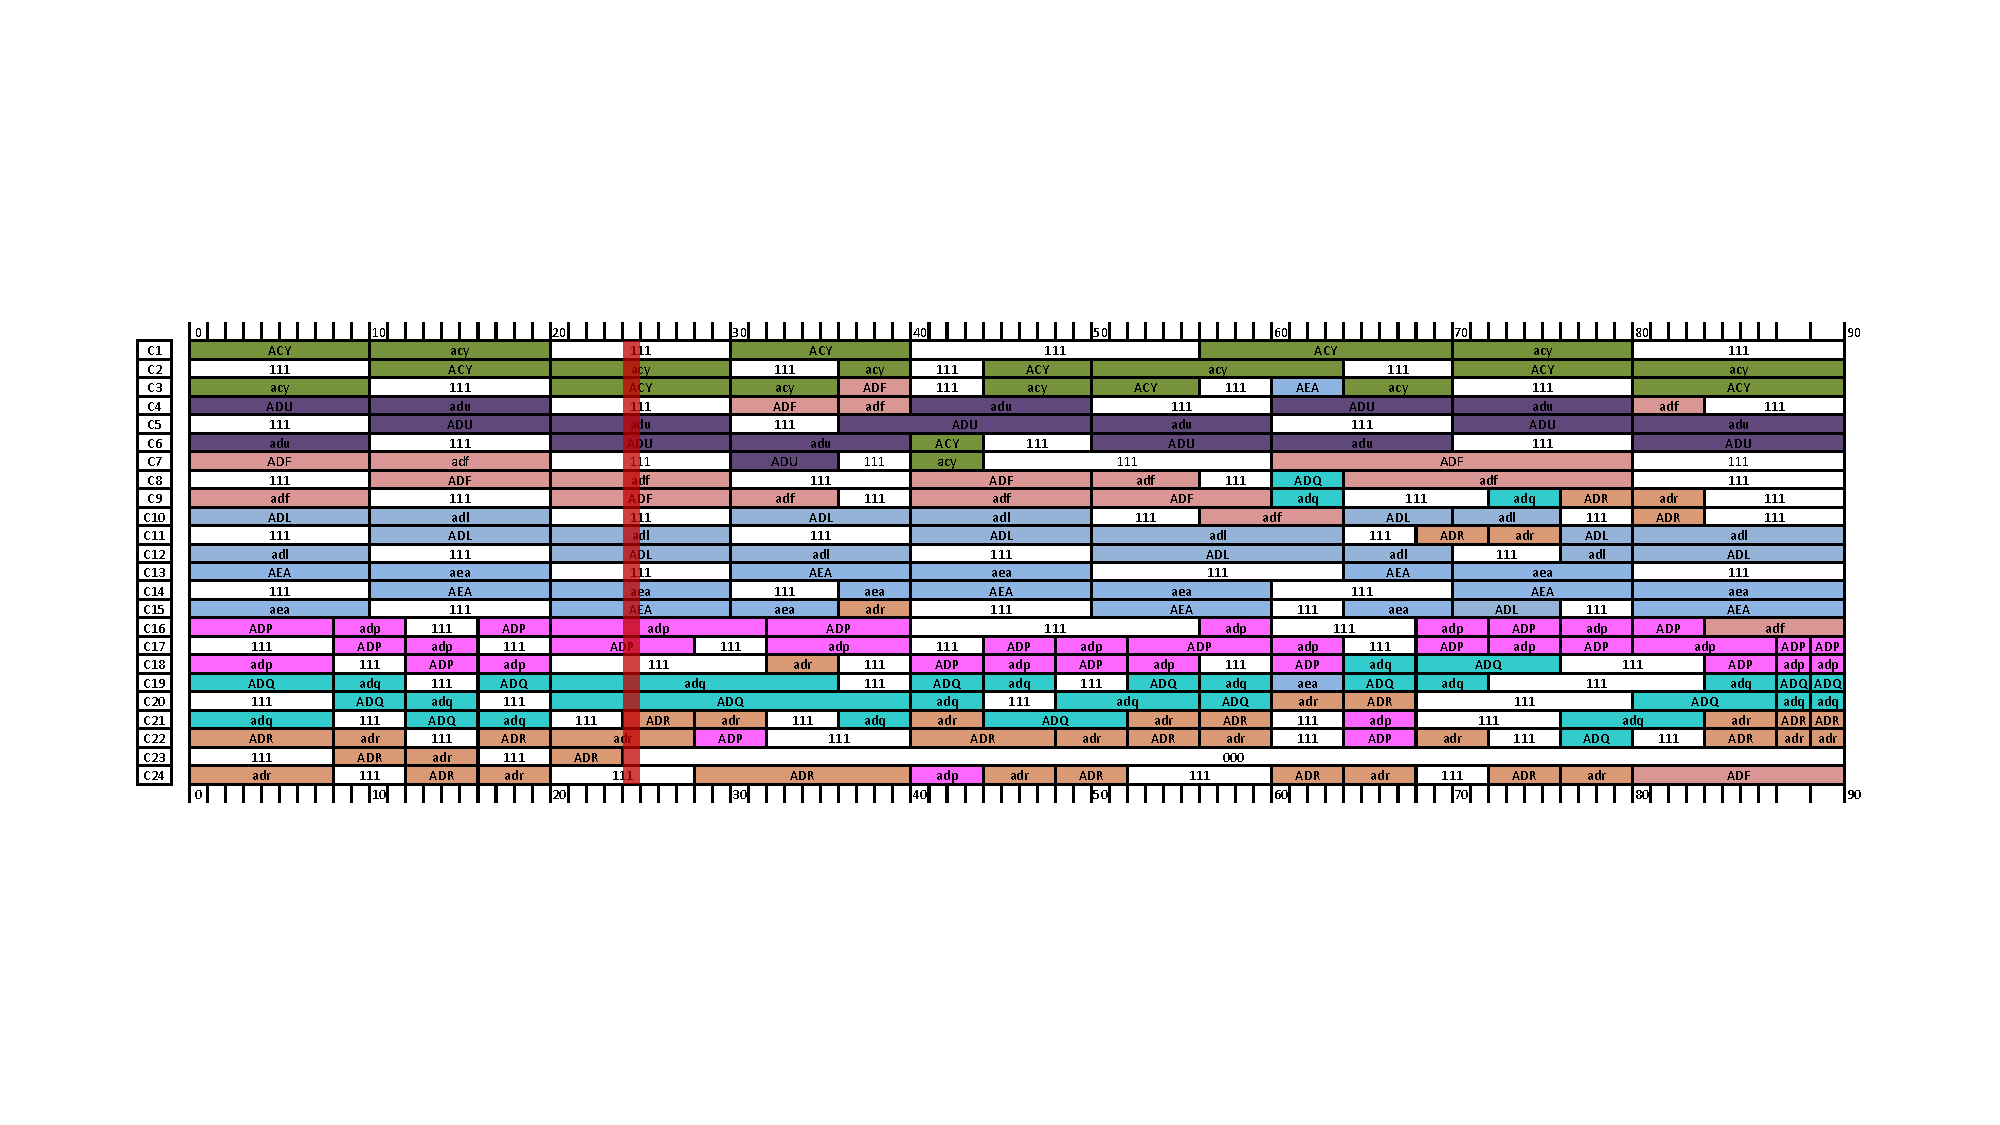
\includegraphics[width=\linewidth]{caso3/caso3-fase2}
	\caption{Solución final (\fasedos{}) para el Caso 3}
	\label{fig:caso3-fase2}
\end{figure}

\subsubsection{Análisis del Caso 4}

En el Caso 4, como ya se ha dicho, no se precisa de ningún controlador imaginario adicional, por lo que el valor del \ref{O1} ya toma el valor máximo en la primera iteración.

La sectorización inicial, planificada como se muestra en la \autoref{fig:caso4-fase0}, consta de un único núcleo con una única sectorización. La incidencia nos dice que esta sectorización ahora se ha desglosado en 4 con diferentes periodos, como muestra la \autoref{fig:caso4-cambio-sectorizacion}. Aquellos sectores que tengan el mismo color indica que son sustituidos por afinidad, y en cursiva se encuentran aquellos que se cierran.

\begin{figure}[!]
	\centering
	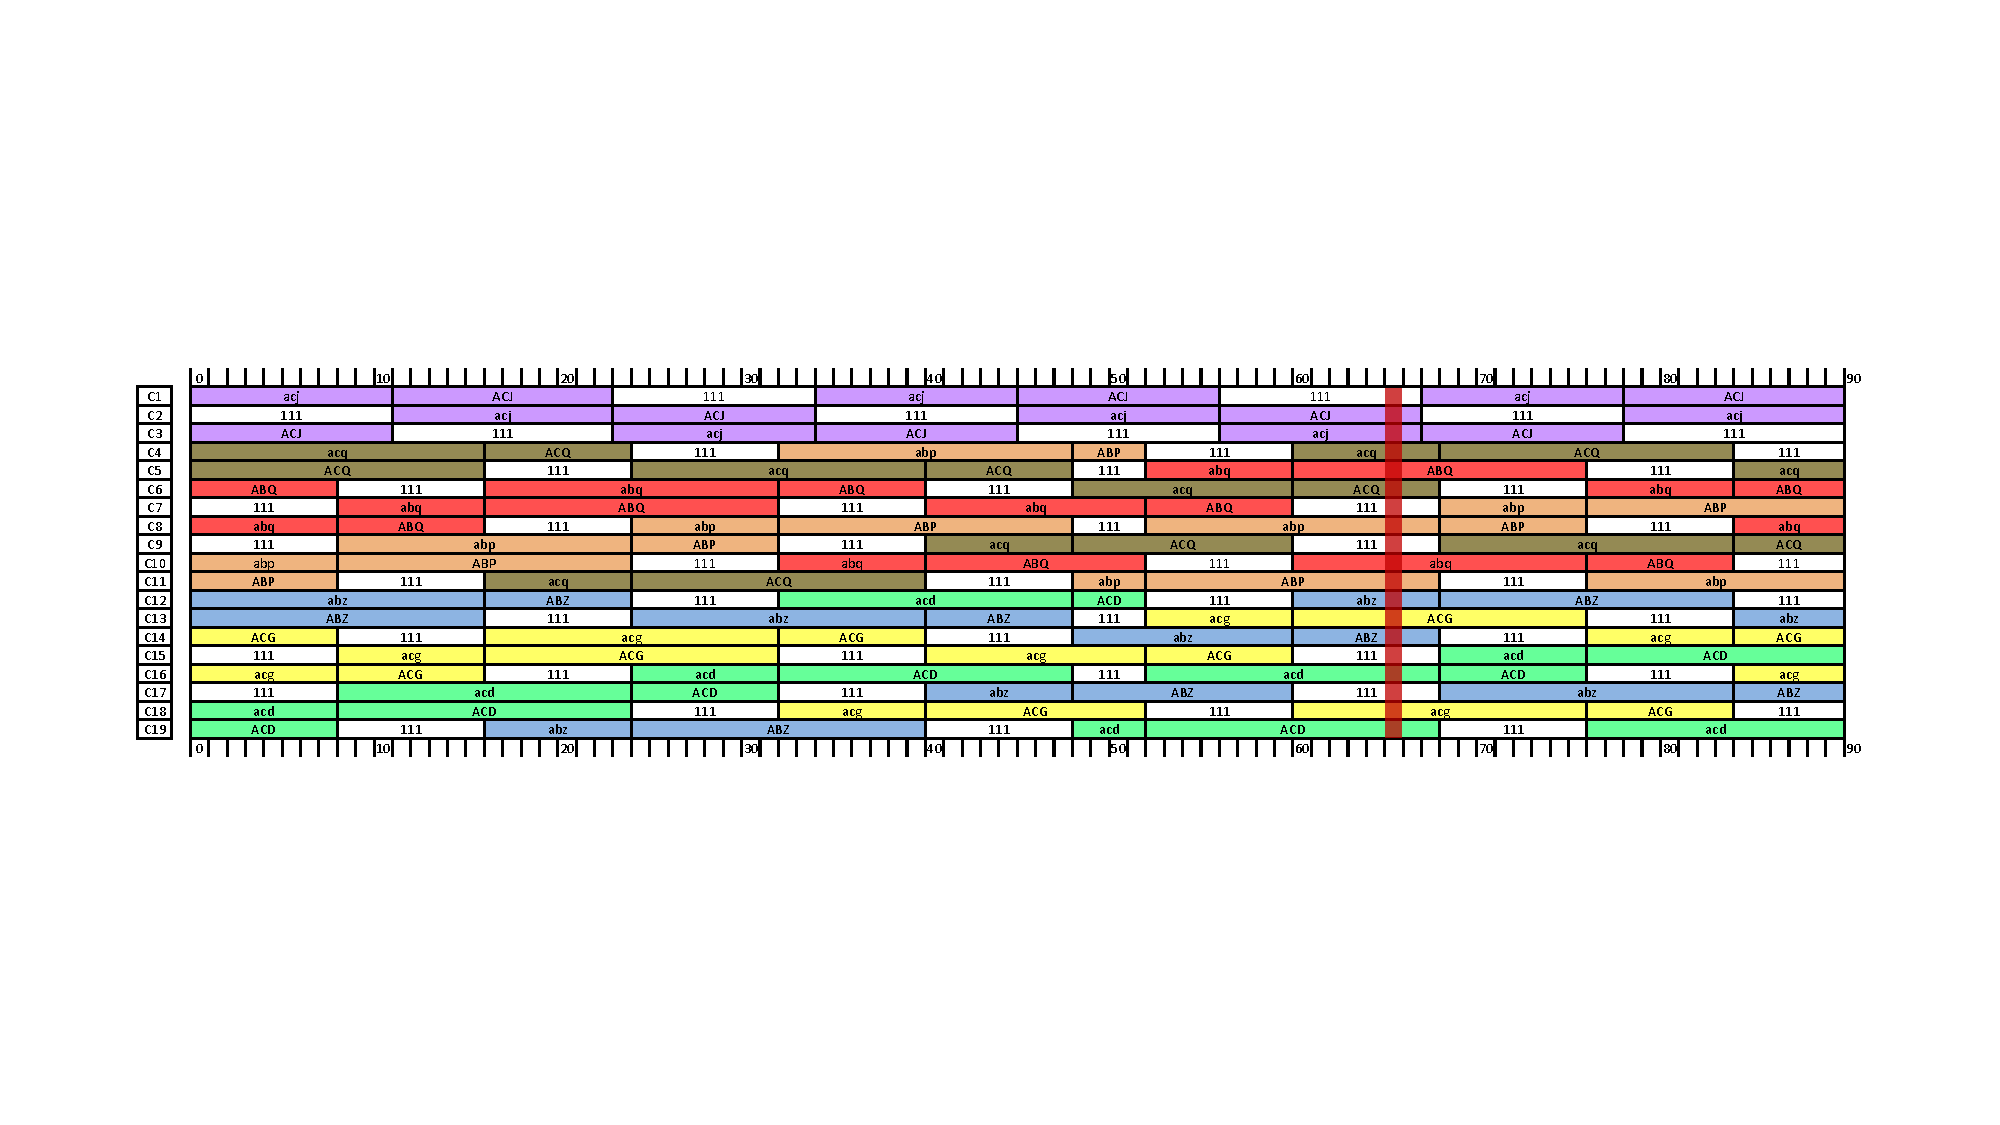
\includegraphics[width=\linewidth]{caso4/caso4-fase0}
	\caption{Planificación inicial del Caso 4}
	\label{fig:caso4-fase0}
\end{figure}

\begin{figure}[!]
	\centering
	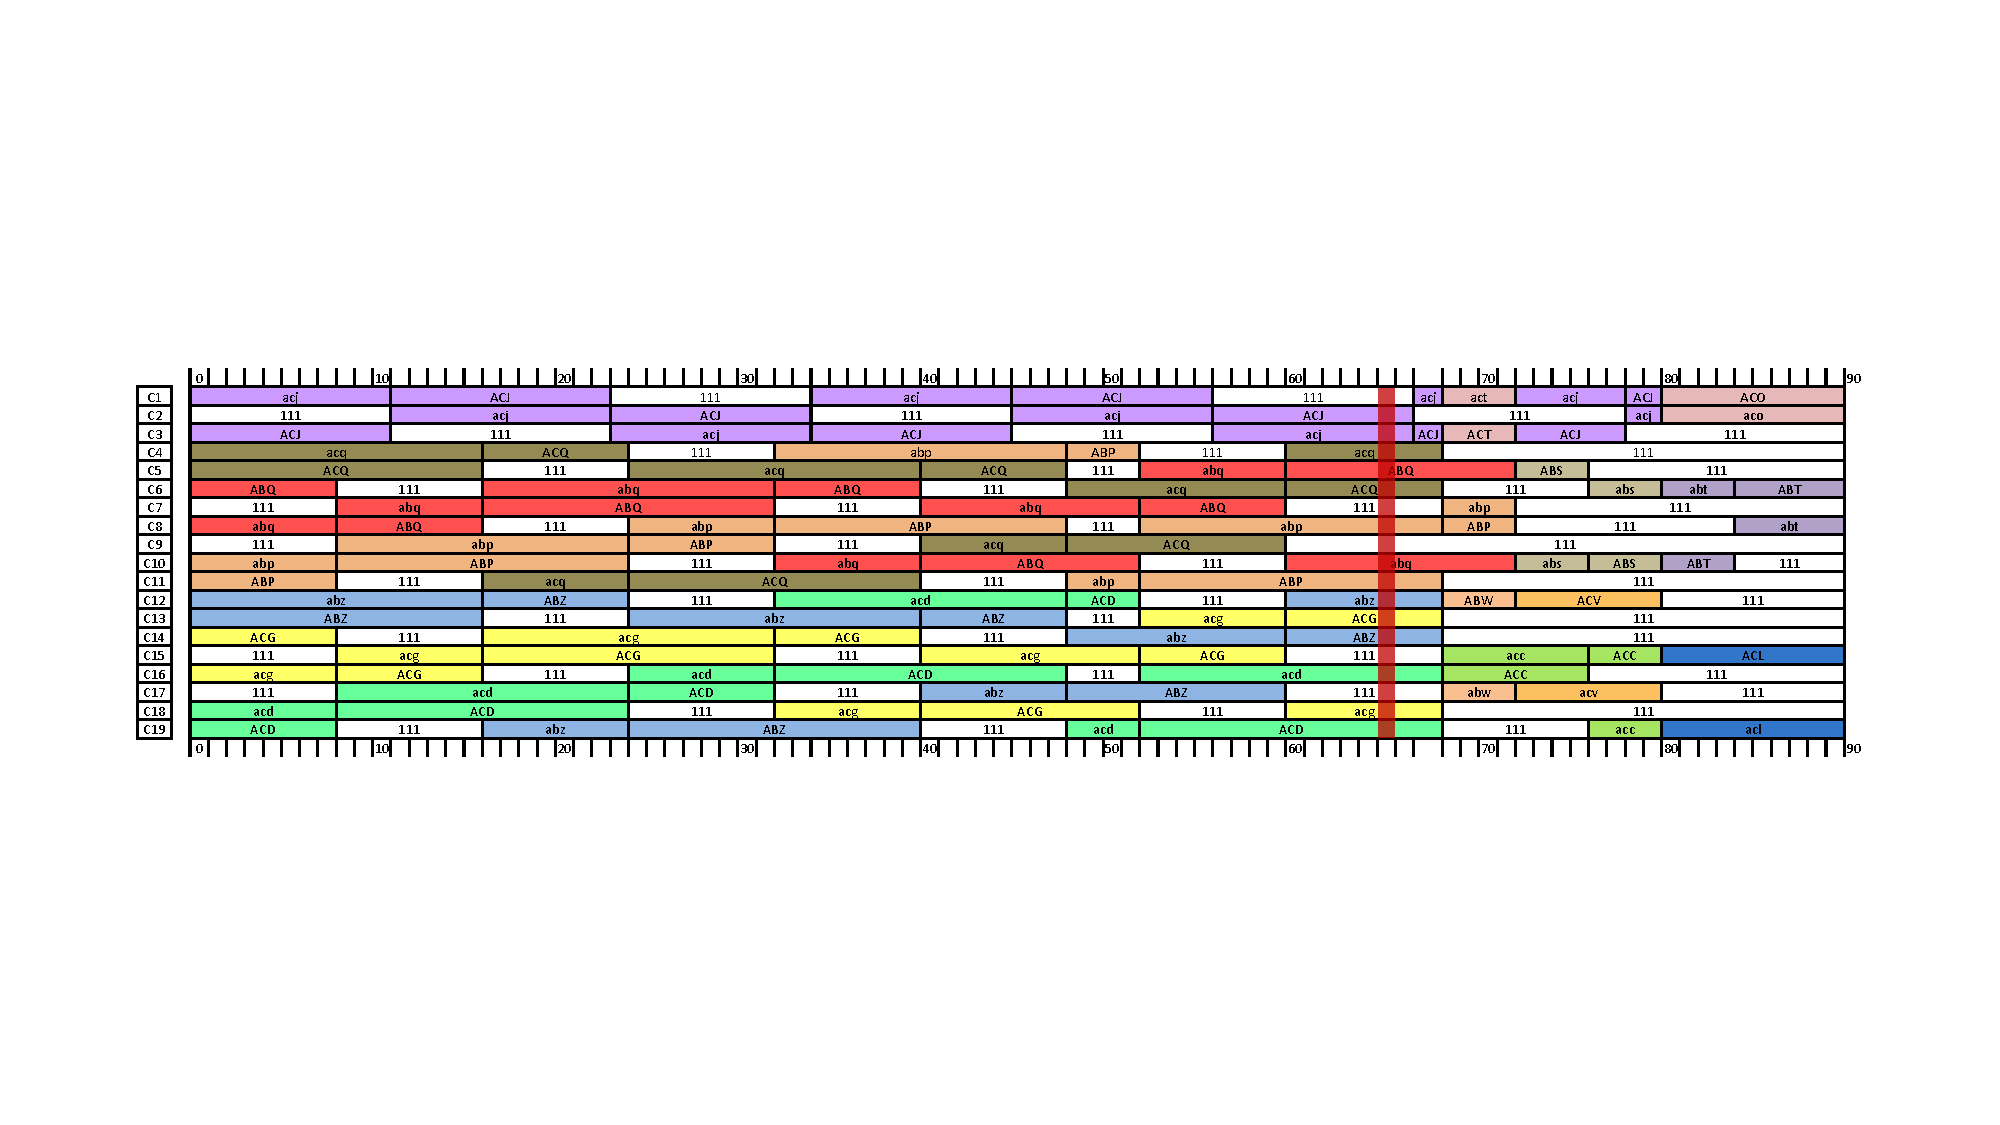
\includegraphics[width=\linewidth]{caso4/caso4-fase1}
	\caption{Solución inicial (\faseuno{}) para el Caso 4}
	\label{fig:caso4-fase1}
\end{figure}

\begin{figure}[!]
	\centering
	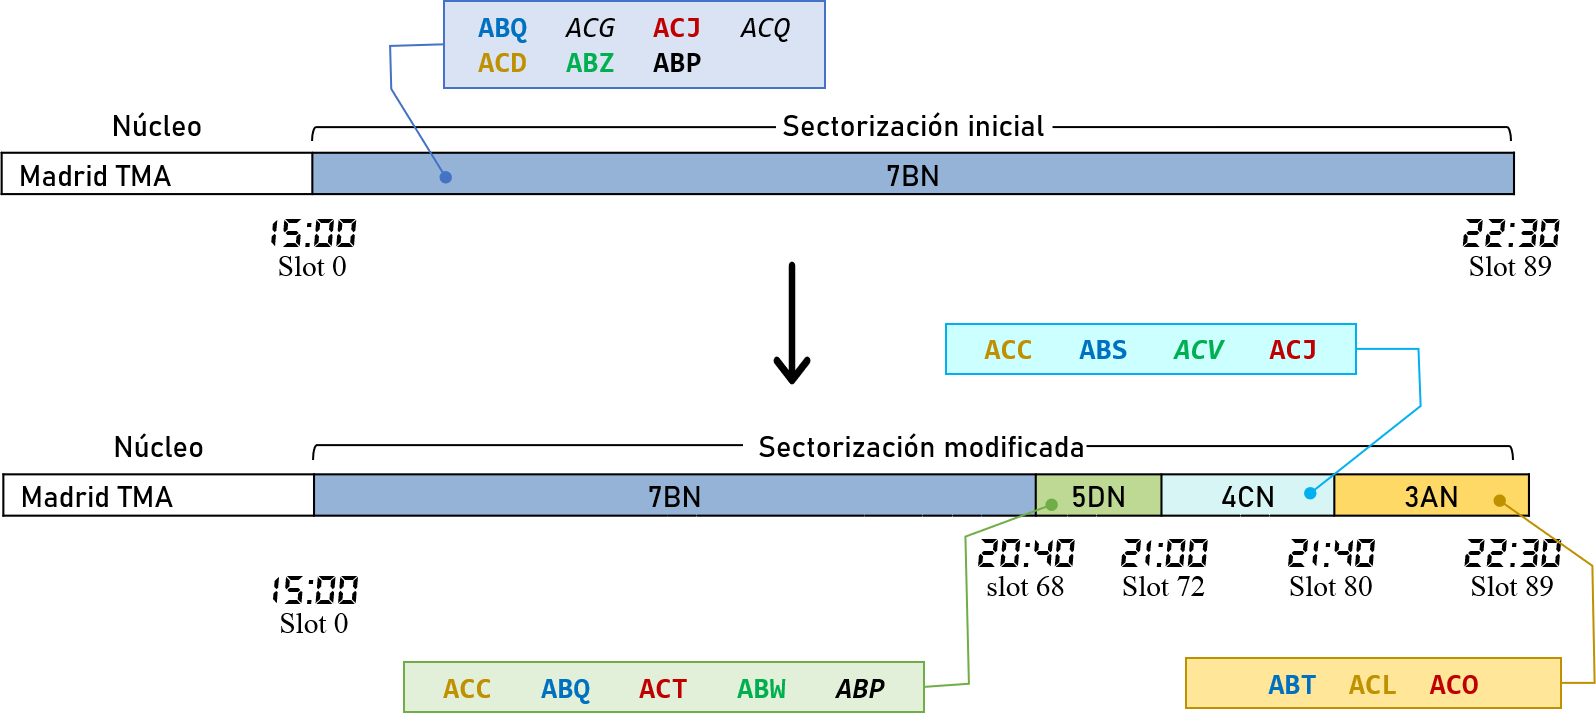
\includegraphics[width=\linewidth]{caso4/cambio-sectorizacion}
	\caption{Esquema del cambio de sectorización que sucede en el Caso 4 y 5}
	\label{fig:caso4-cambio-sectorizacion}
\end{figure}

Por ejemplo, el sector ACJ se cierra durante el primer periodo y es sustituido por el afín ACT; en el segundo periodo el sector ACJ vuelve a abrirse y en el último periodo nuevamente se cierra. 

Los sectores ACQ y ACG se cierran a partir del segundo tramo incluido, ABP a partir del tercero.

Como podemos observar en la \autoref{fig:caso4-fase1}, todos los sectores o bien se cierran o bien son sustituidos por otro afín por lo que no hay necesidad de añadir nuevas filas a la planificación de la solución inicial.

Una posible solución final, resultante de la \fasedos{}, es la de la \autoref{fig:caso4-fase2-vns} que, como podemos ver, es de una calidad notable, donde se incumple únicamente la restricción \ref{RD:3:porcentaje-min-descanso} en 9 ocasiones, con una similitud a los estadillos muy buena, que permite además disminuir el número de controladores necesarios para planificar las nuevas contingencias a partir de la incidencia a dos controladores menos, y a partir del segundo periodo en otros 7. Un total de 9 controladores menos de la solución inicial. Lógicamente, estos controladores no son eliminados de la planificación puesto que tienen carga de trabajo antes de la incidencia.

En el caso de SA (\autoref{fig:caso4-fase2-sa}), la calidad de la solución es muy similar en cuanto a restricciones incumplidas como a valores de fitness. Sí cabe destacar que el VNS llega a esta solución en mucho menos tiempo que el SA, este último en 7.5 minutos frente a los 2.8 del VNS.

\begin{figure}[!]
	\centering
	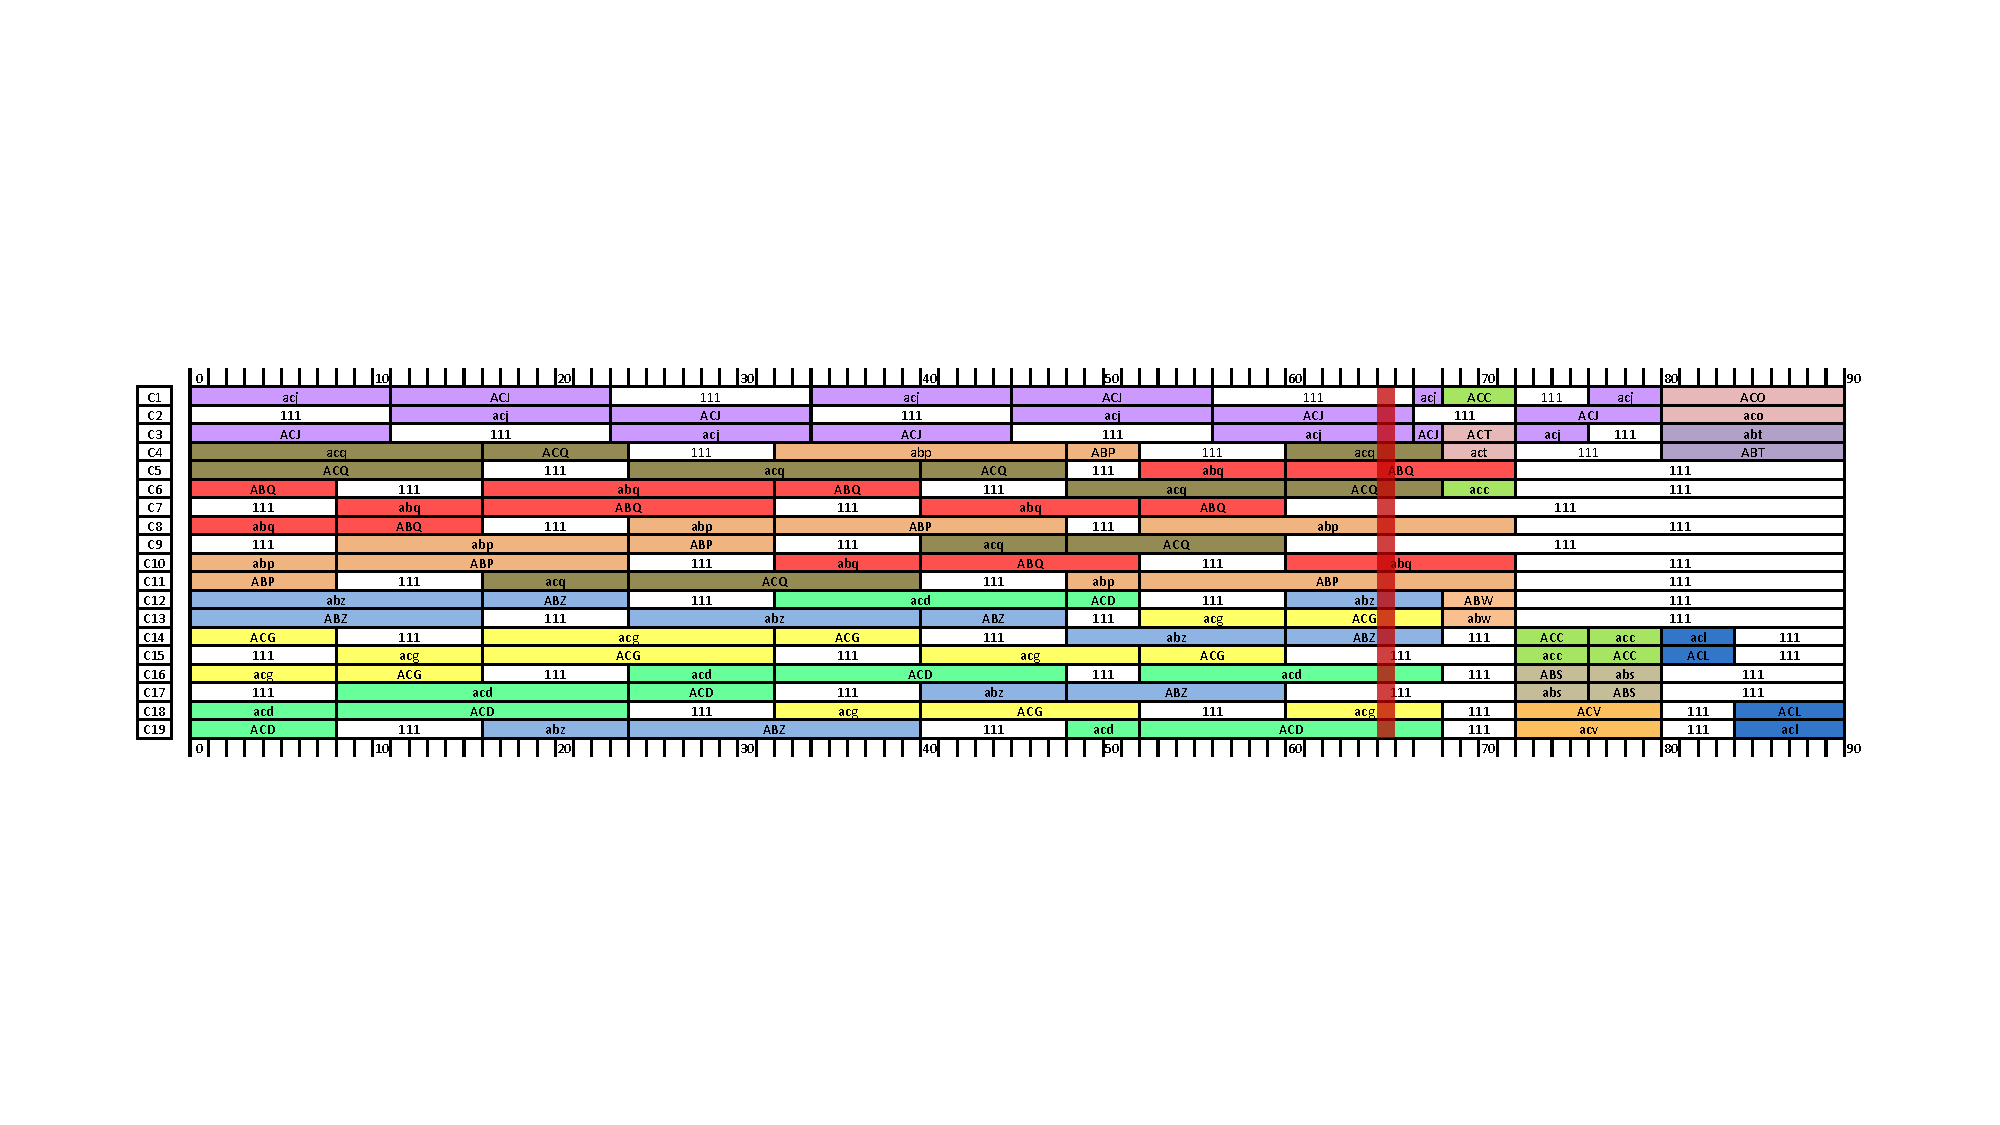
\includegraphics[width=\linewidth]{caso4/caso4-fase2-vns}
	\caption{Solución final (\fasedos{}) para el Caso 4 empleando VNS}
	\label{fig:caso4-fase2-vns}
\end{figure}

\begin{figure}[!]
	\centering
	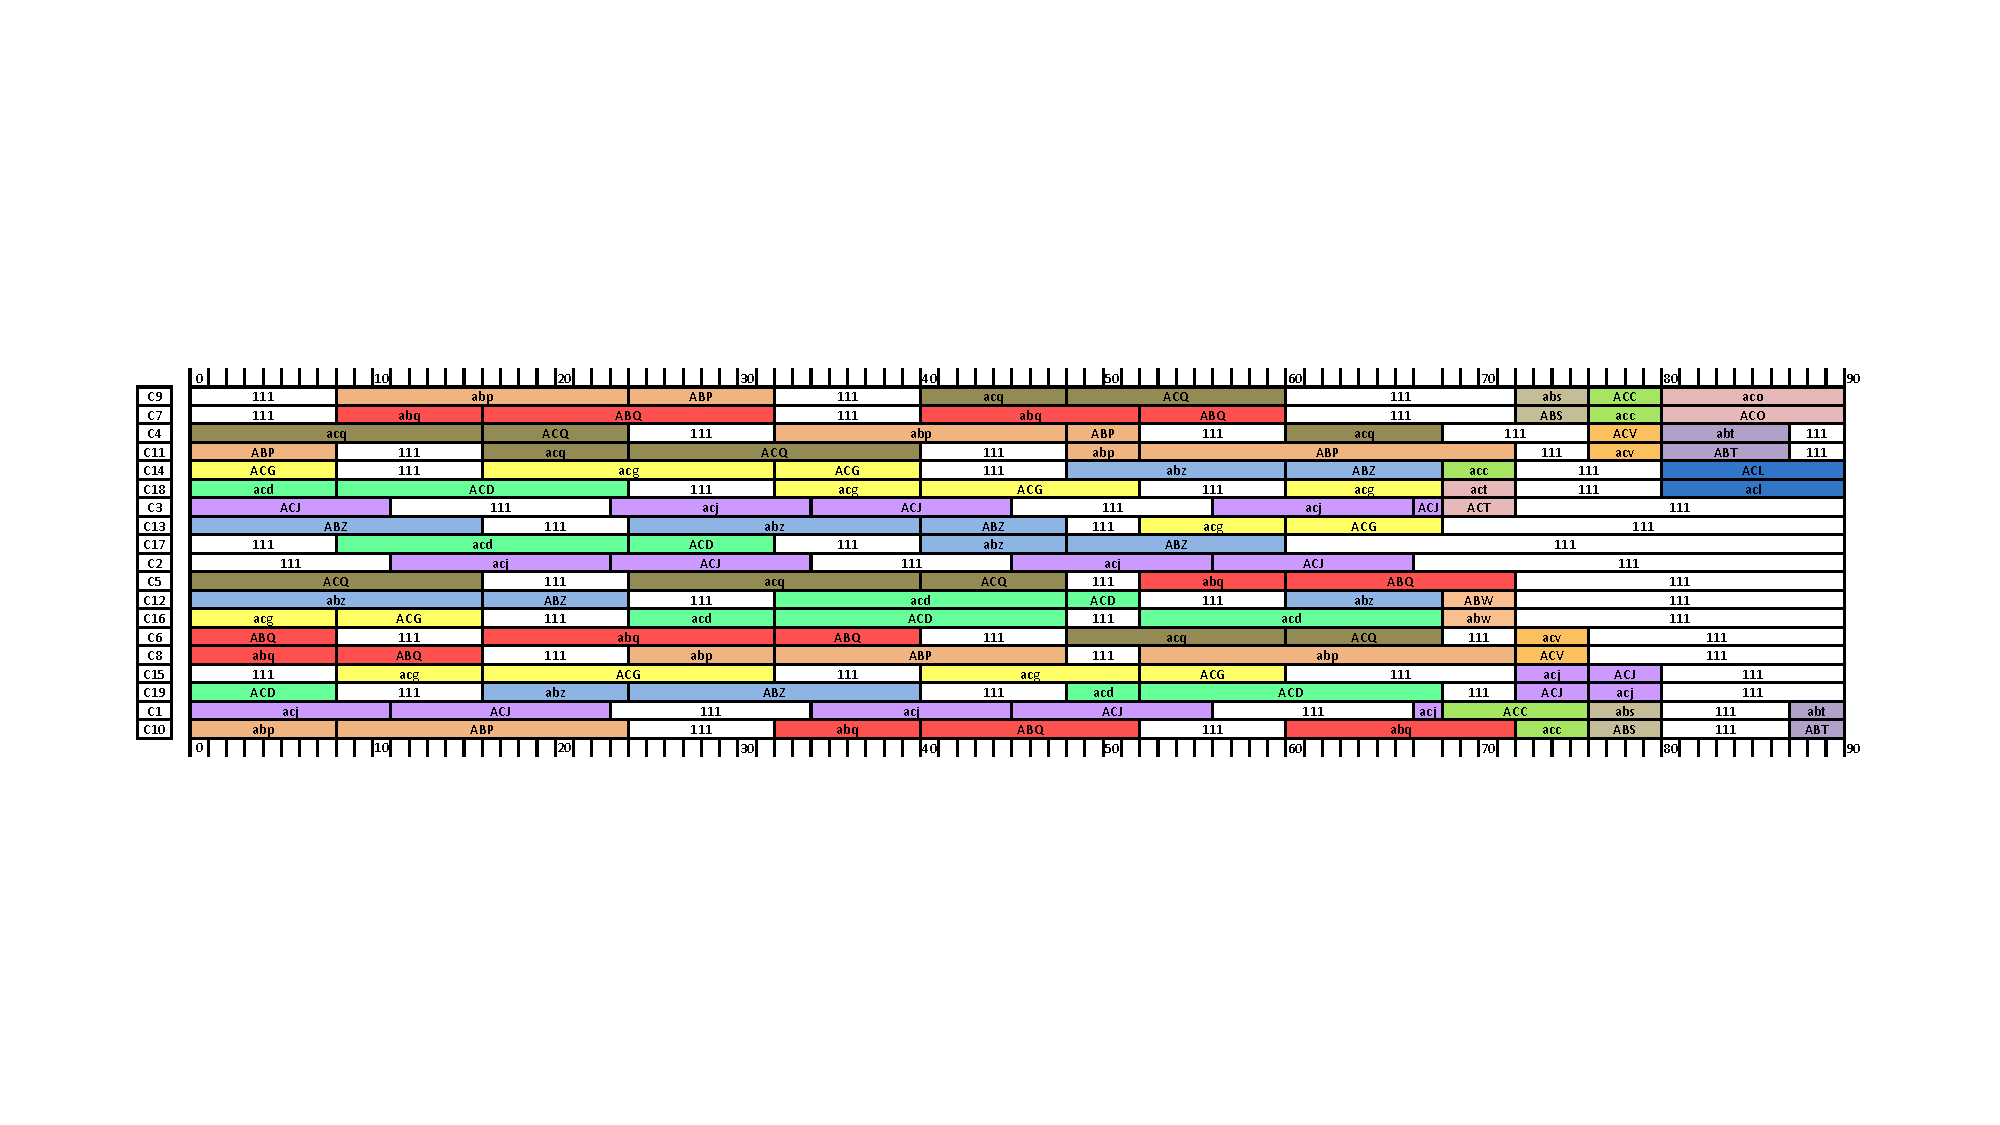
\includegraphics[width=\linewidth]{caso4/caso4-fase2-sa}
	\caption{Solución final (\fasedos{}) para el Caso 4 empleando SA}
	\label{fig:caso4-fase2-sa}
\end{figure}

\subsubsection{Análisis del Caso 5}

La planificación inicial del Caso 5 es la misma que la del caso anterior, cambiando el momento del incidente al slot 30 (véase la \autoref{fig:caso5-fase0}).

\begin{figure}[!]
	\centering
	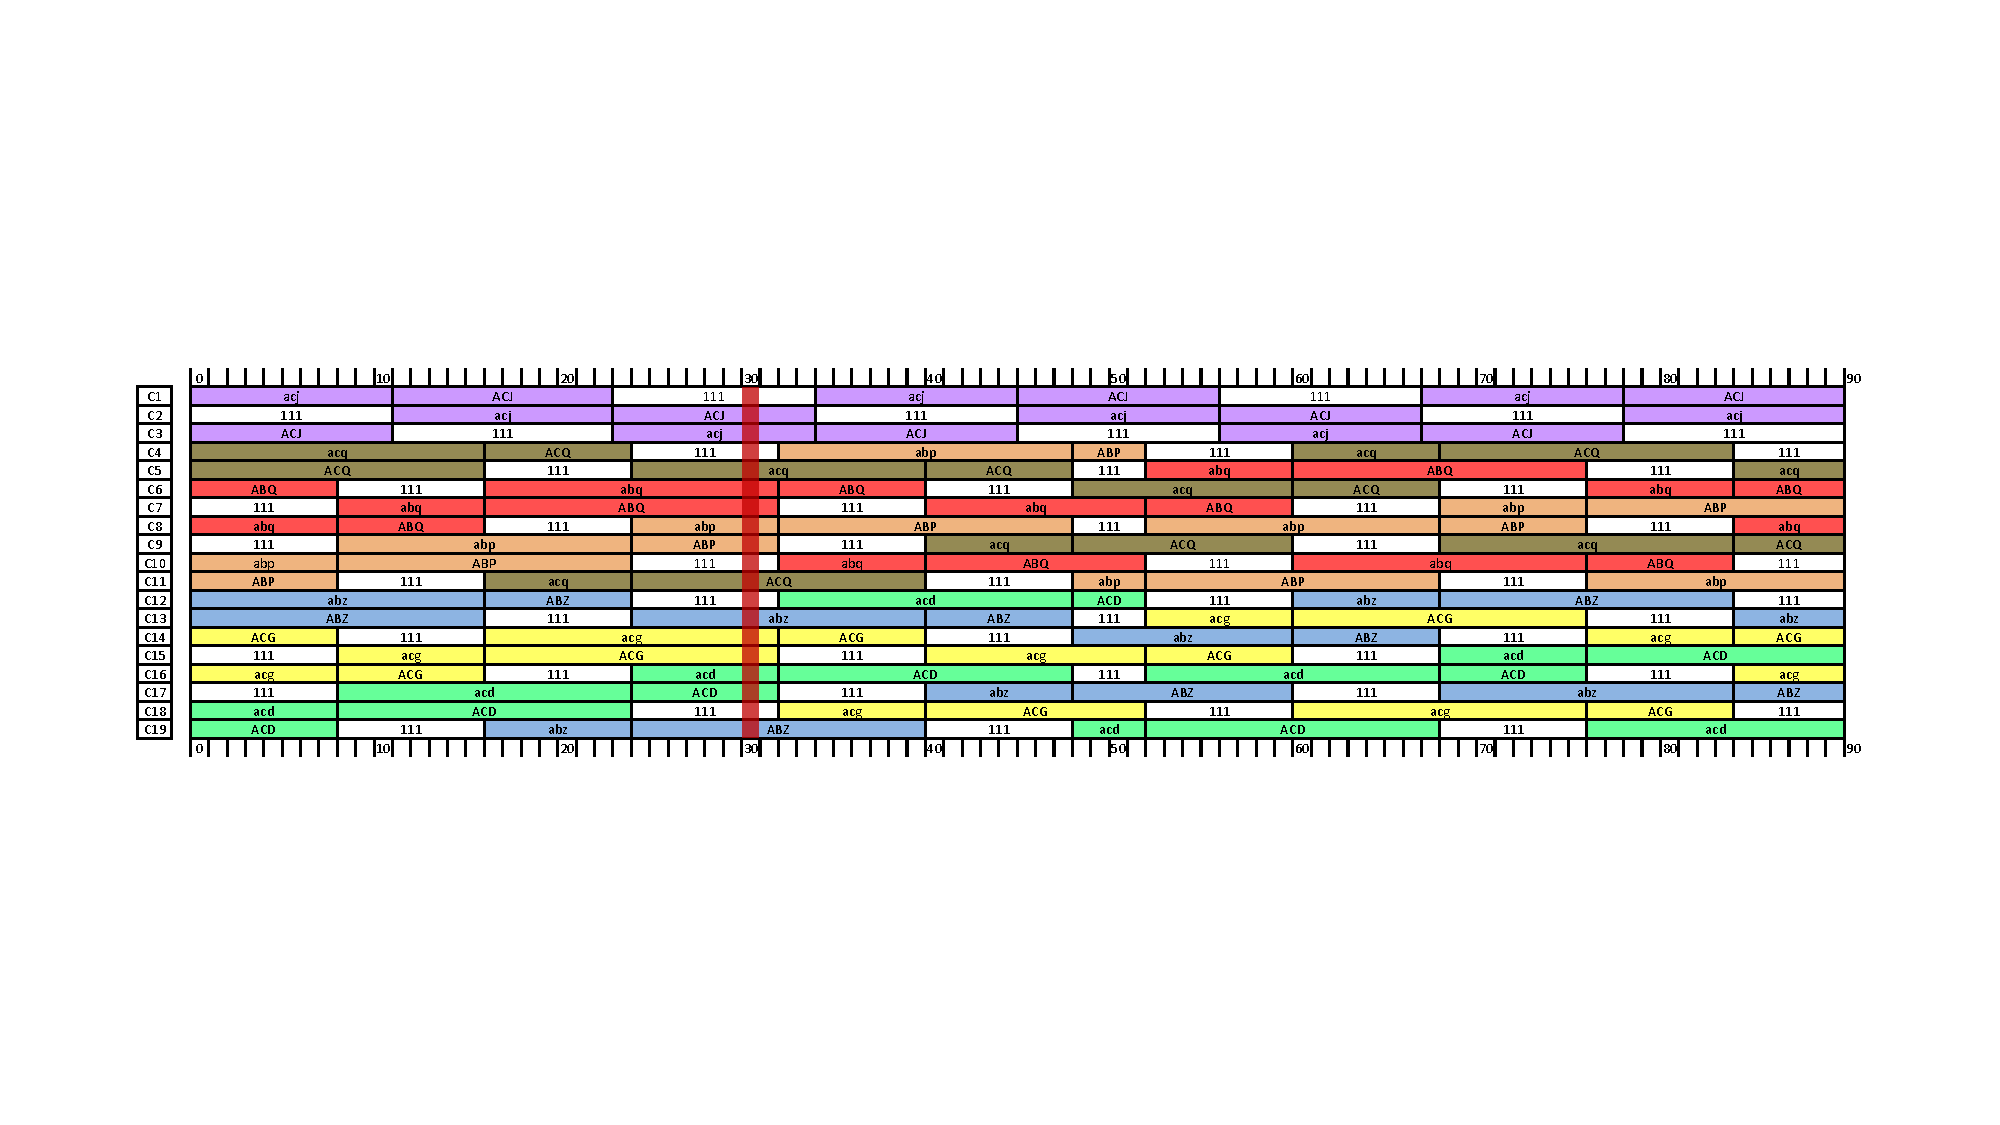
\includegraphics[width=\linewidth]{caso5/caso5-fase0}
	\caption{Planificación inicial del Caso 5}
	\label{fig:caso5-fase0}
\end{figure}

La \faseuno{} obtiene como resultado la misma que en el Caso 4, añadiéndole un controlador imaginario para suplir la carencia del controlador que se da de baja a partir del slot 30. Se produce una alta, por lo que se añade también un controlador, pero en este caso no imaginario, puesto que es un recurso que ya se conoce como disponible. La solución inicial se muestra en la \autoref{fig:caso5-fase1}.

\begin{figure}[!]
	\centering
	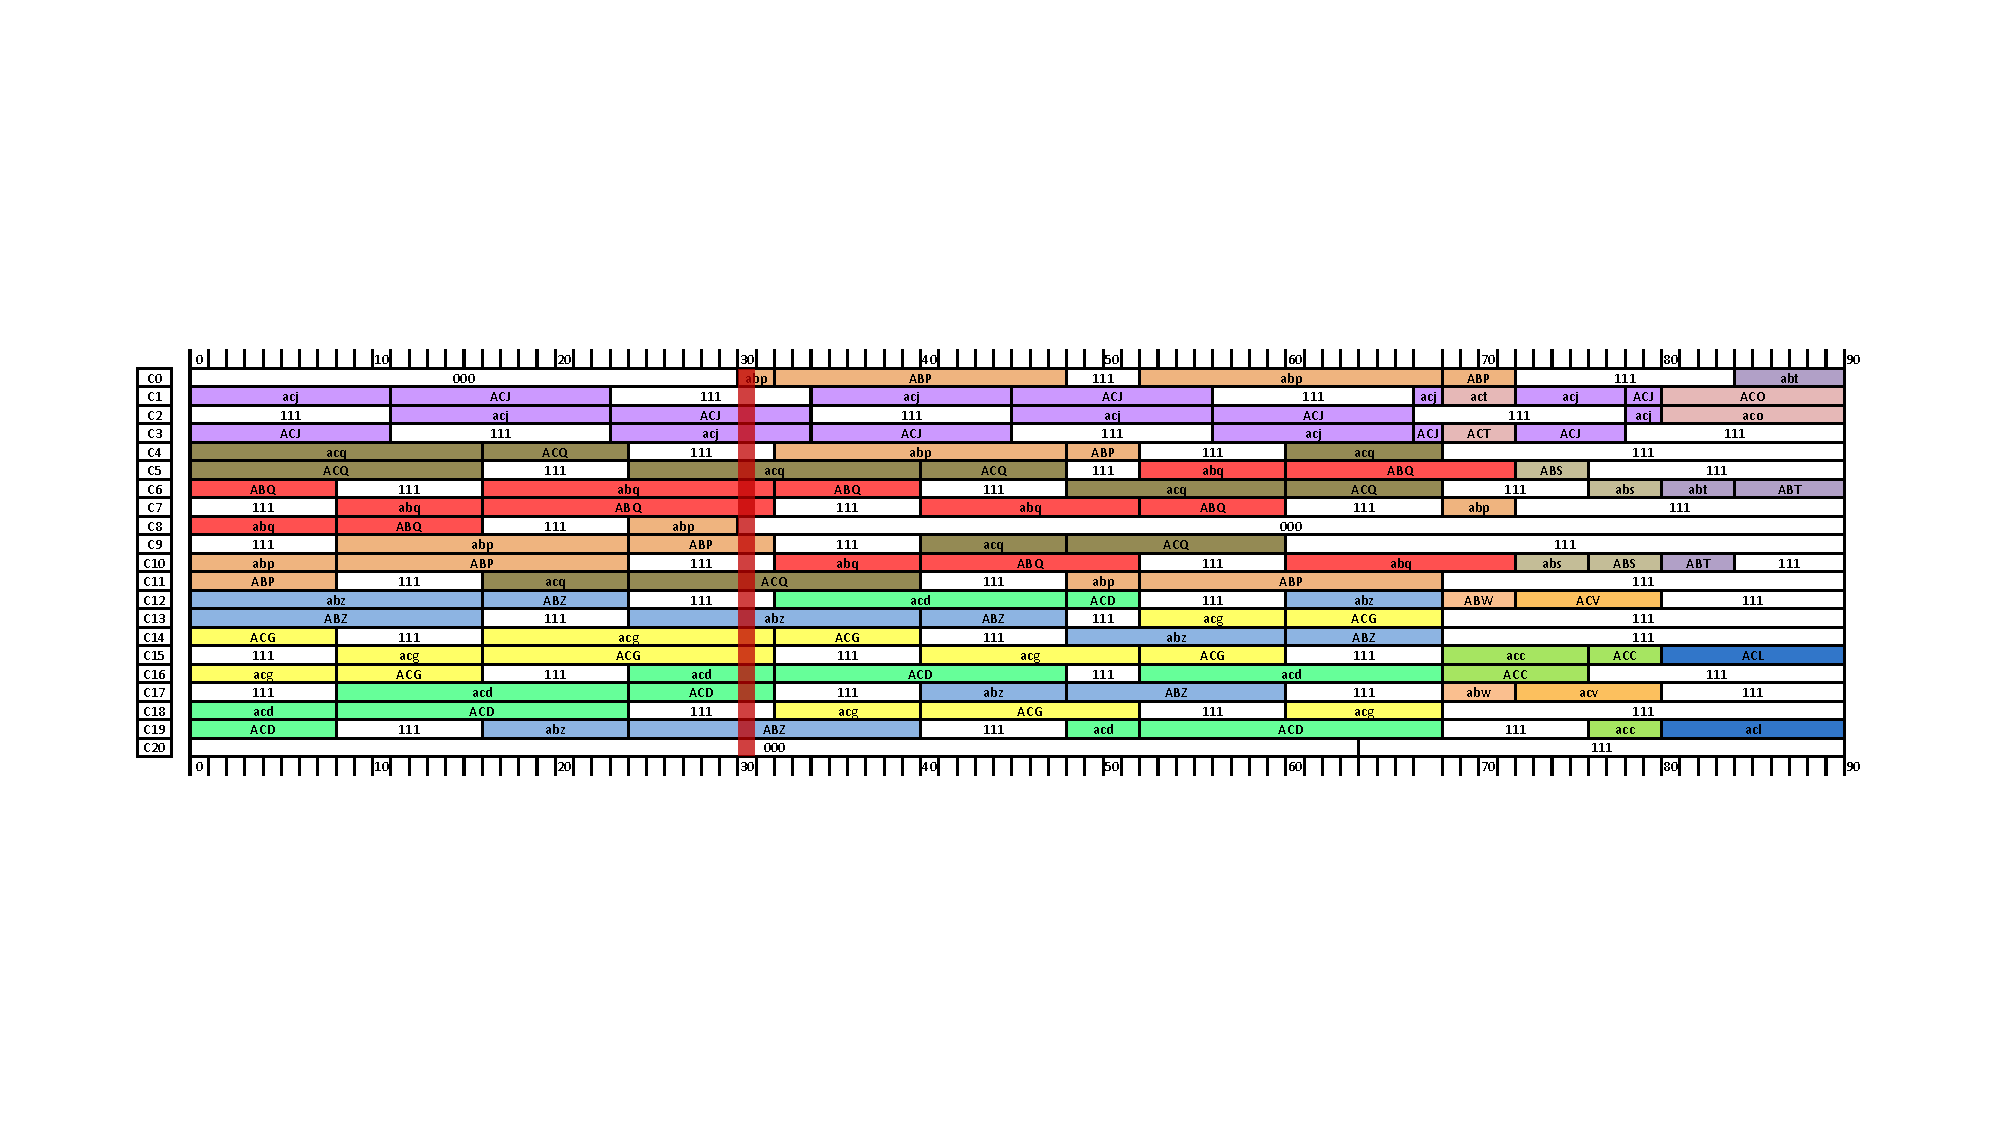
\includegraphics[width=\linewidth]{caso5/caso5-fase1}
	\caption{Solución inicial (\faseuno{}) para el Caso 5}
	\label{fig:caso5-fase1}
\end{figure}

La idea es que se reorganice toda la planificación a partir del momento de la baja del controlador para poder realizar el trabajo sin el controlador de baja, junto con realizar las adaptaciones a la nueva sectorización de la mejor forma posible.

La \autoref{fig:caso5-fase2-vns} representa un posible resultado alcanzado con nuestro VNS. Como podemos ver, sí es capaz de eliminar el controlador imaginario adicional, a expensas de incumplir la restricción \ref{R:5:max-trabajo-continuado} en dos ocasiones, algo que no sucede en la solución obtenida con SA de la \autoref{fig:caso5-fase2-sa}. Por ello, el objetivo \ref{O2} es inferior en valor en VNS.

Respecto al objetivo \ref{O3}, ambas metaheurísticas obtienen resultados similares, aunque en relación al \ref{O4}, la similitud con las plantillas es significativamente superior la del VNS.

\begin{figure}[!]
	\centering
	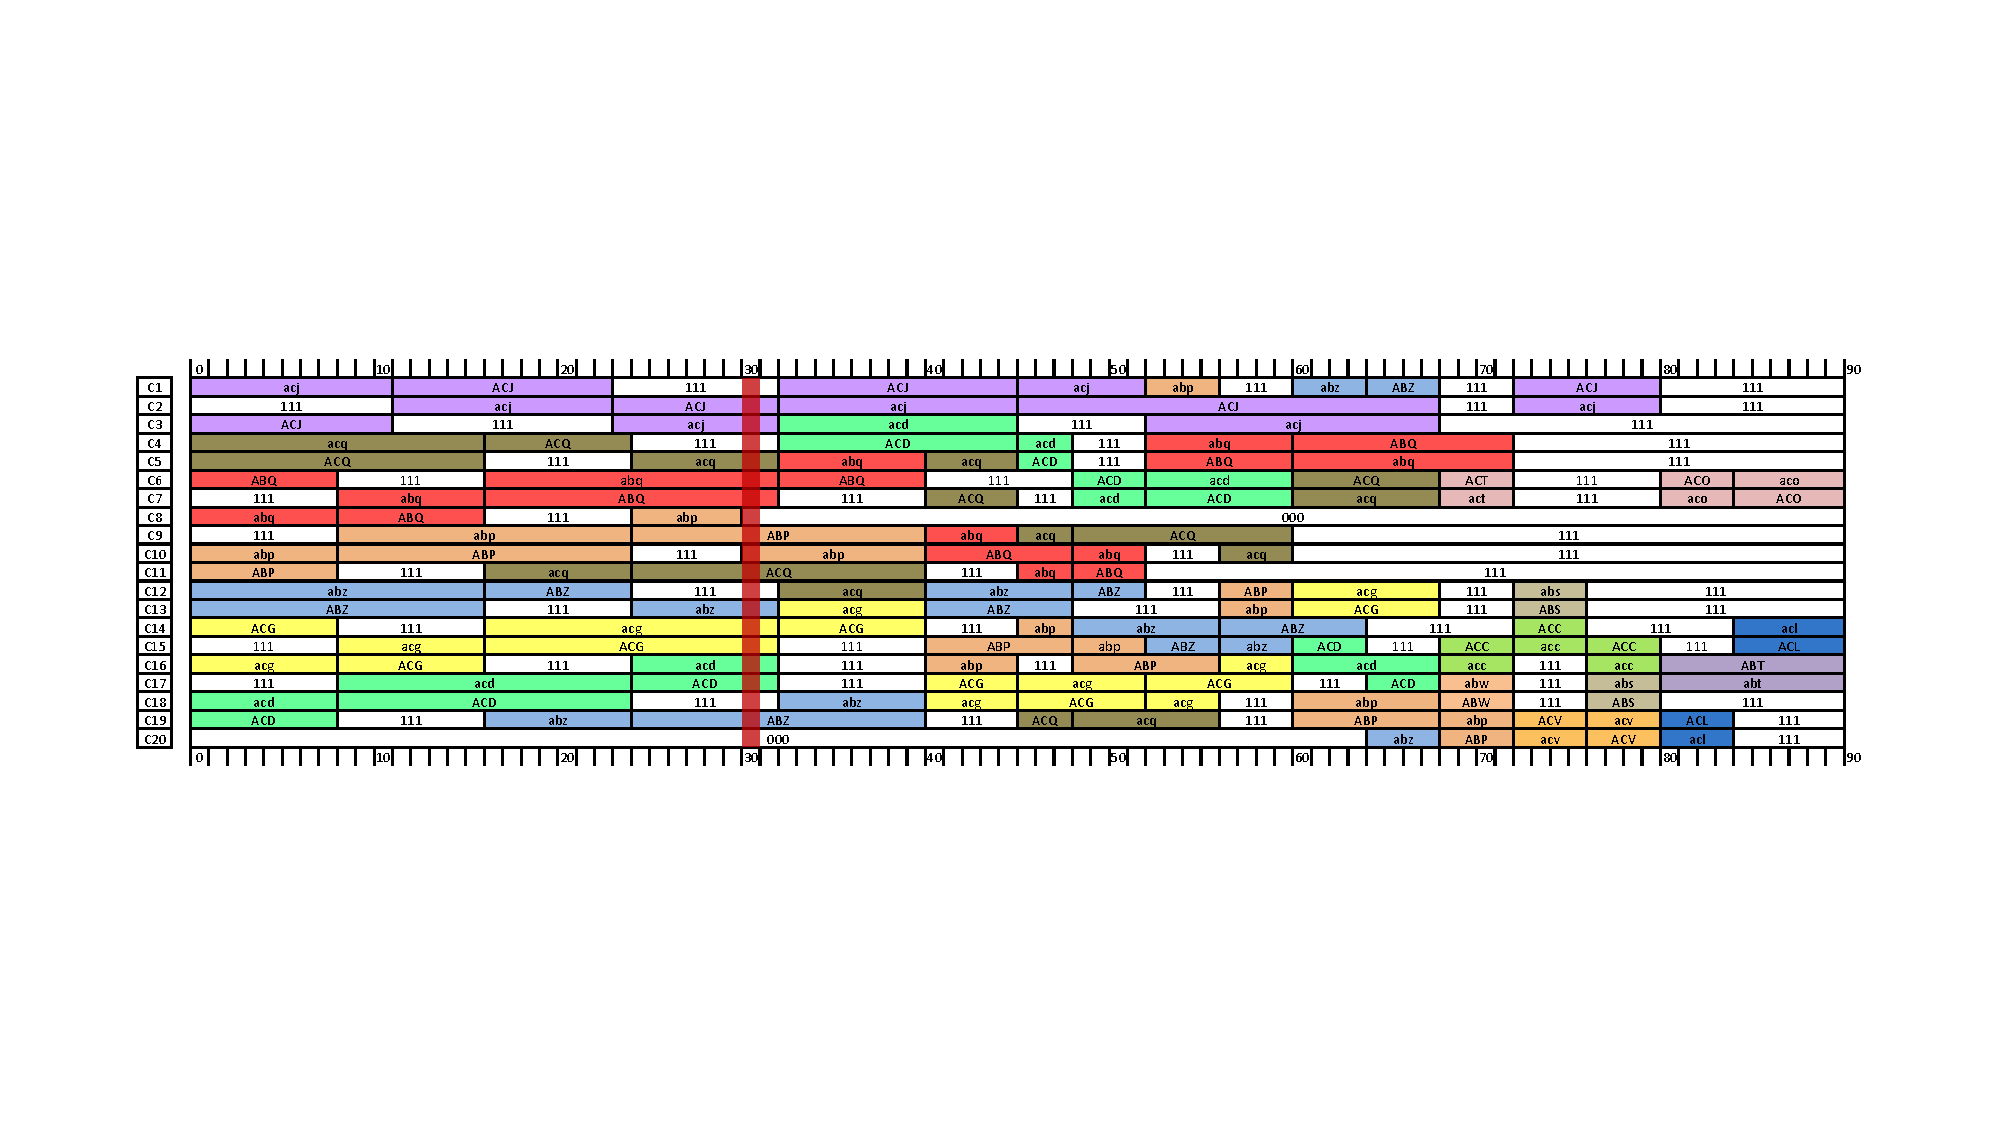
\includegraphics[width=\linewidth]{caso5/caso5-fase2-vns}
	\caption{Solución final (\fasedos{}) para el Caso 5 empleando VNS}
	\label{fig:caso5-fase2-vns}
\end{figure}

\begin{figure}[!]
	\centering
	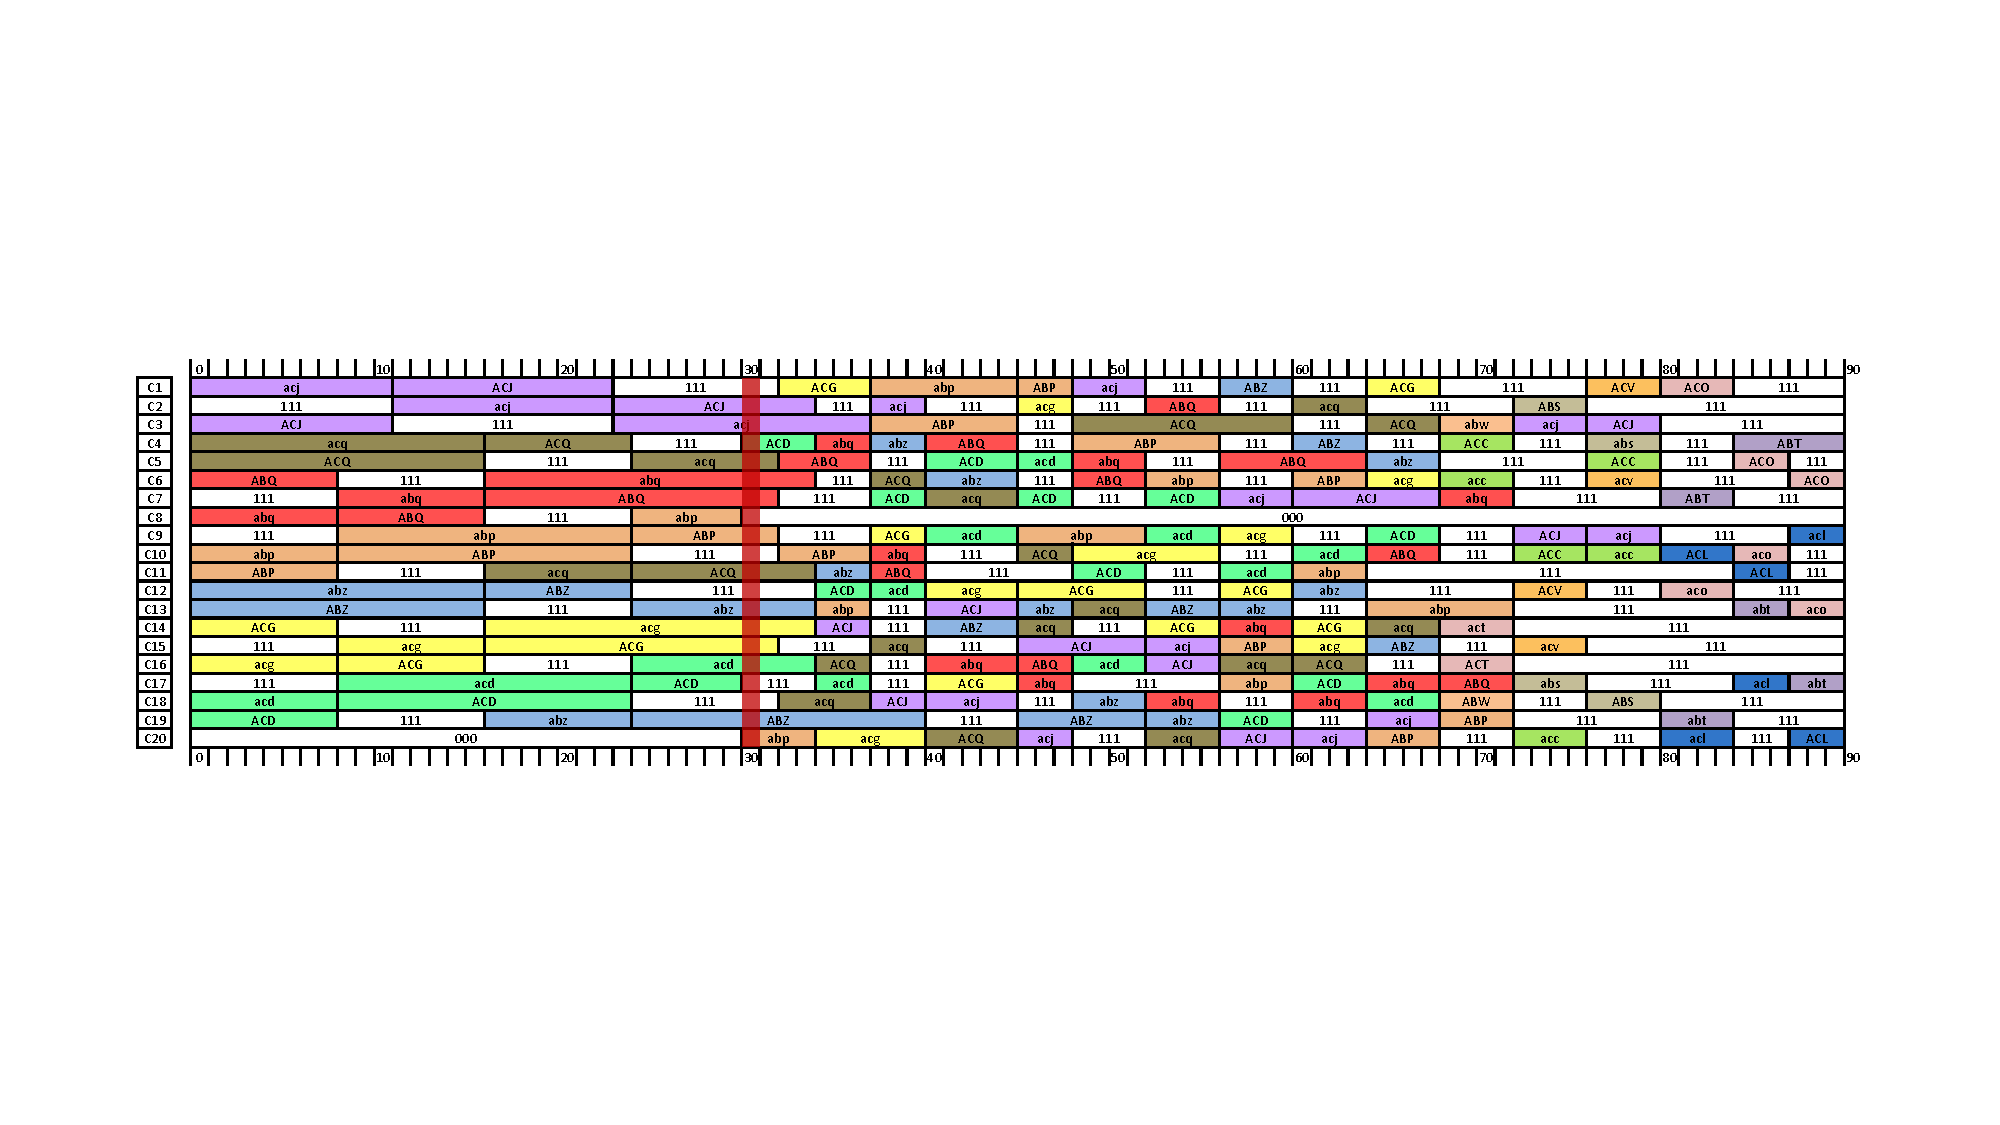
\includegraphics[width=\linewidth]{caso5/caso5-fase2-sa}
	\caption{Solución final (\fasedos{}) para el Caso 5 empleando SA}
	\label{fig:caso5-fase2-sa}
\end{figure}
\subsubsection{Análisis del Caso 6}

Nuevamente, la planificación inicial es la misma que la del Caso 4, pero en este caso el momento del cambio es antes, en el slot 32 (véase la \autoref{fig:caso6-fase0}).

La incidencia de este caso es consiste en un cambio de sectorización, no obstante, diferente al del Caso 4, mostrado en la \autoref{table:D:caso6-modif}. Implica la apertura de un mayor número de sectores, por lo que debido a esto, se ve necesario el uso de una plantilla $3 \times 1$ que introduce 3 controladores imaginarios (véase la \autoref{fig:caso6-fase1}).

\begin{figure}[!]
	\centering
	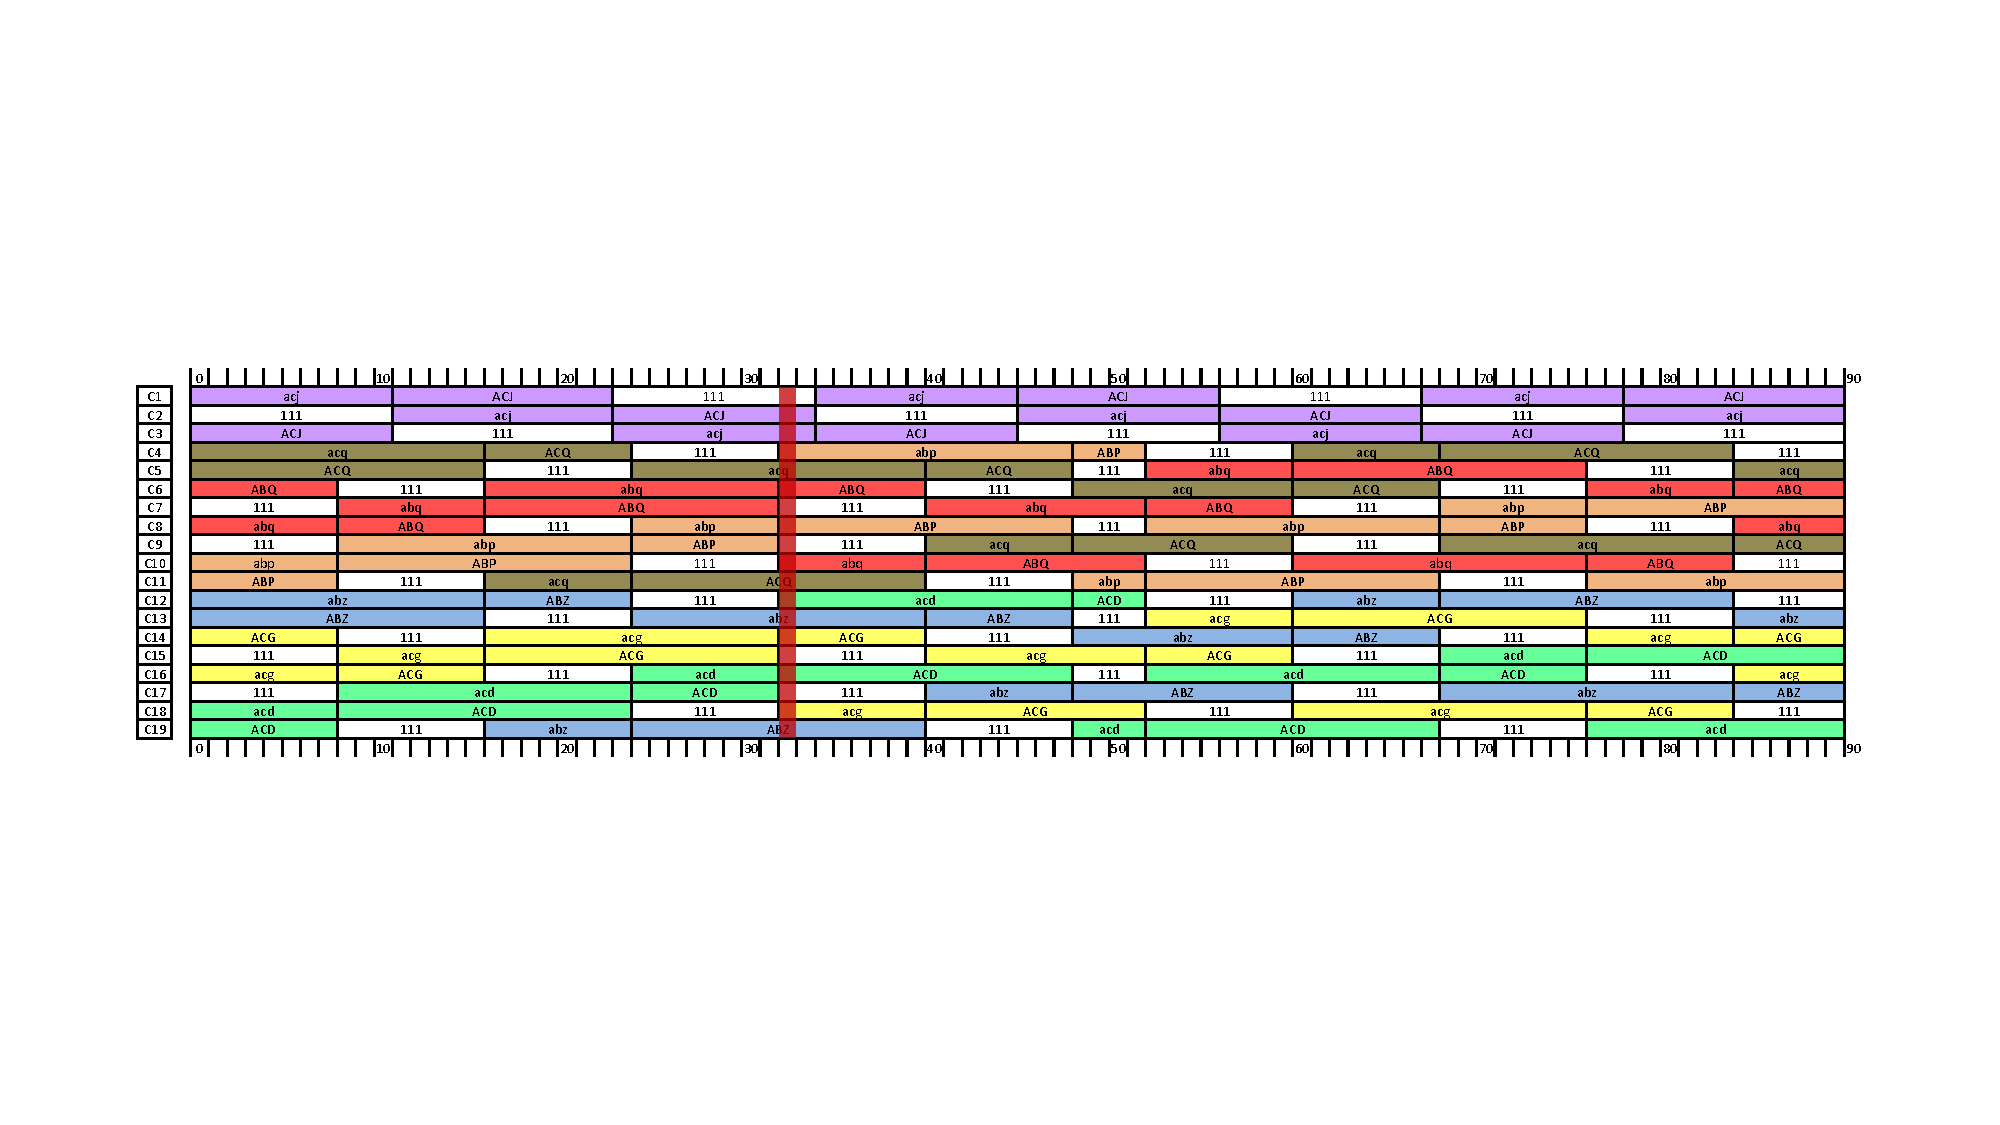
\includegraphics[width=\linewidth]{caso6/caso6-fase0}
	\caption{Planificación inicial para el Caso 6}
	\label{fig:caso6-fase0}
\end{figure}

\begin{figure}[!]
	\centering
	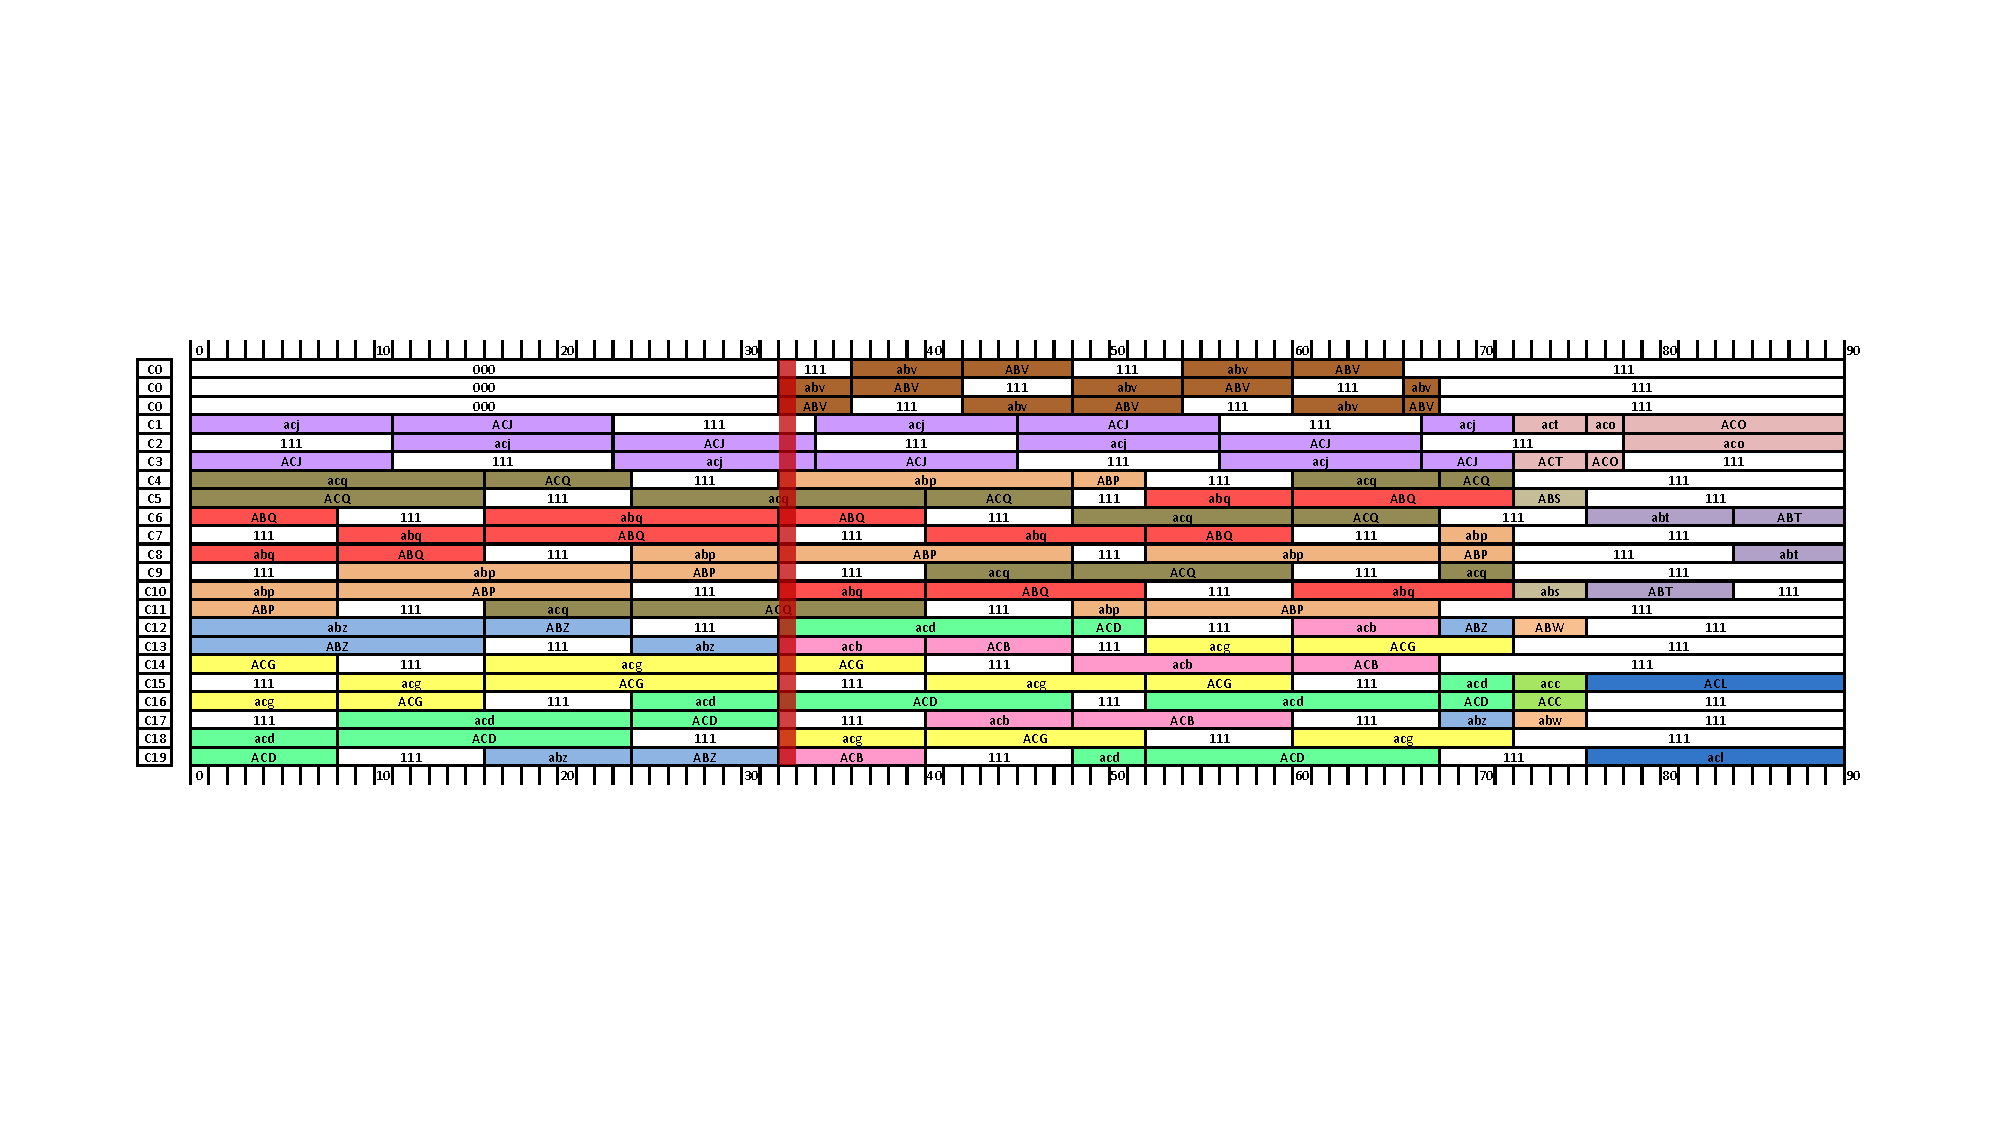
\includegraphics[width=\linewidth]{caso6/caso6-fase1}
	\caption{Solución inicial (\faseuno{}) para el Caso 6}
	\label{fig:caso6-fase1}
\end{figure}

En la \fasedos{} podemos apreciar visualmente que tanto el VNS (\autoref{fig:caso6-fase2-vns}) como el SA (\autoref{fig:caso6-fase2-sa}) logran resultados similares para los tres primeros objetivos, \ref{O1}, \ref{O2}, \ref{O3}, aunque en el caso del cuarto, podemos observar cómo el SA obtiene una mayor similitud con los estadillos a partir del momento del cambio. Por esta razón, el valor global del fitness en la solución del SA es mejor que en el VNS.

\begin{figure}[!]
	\centering
	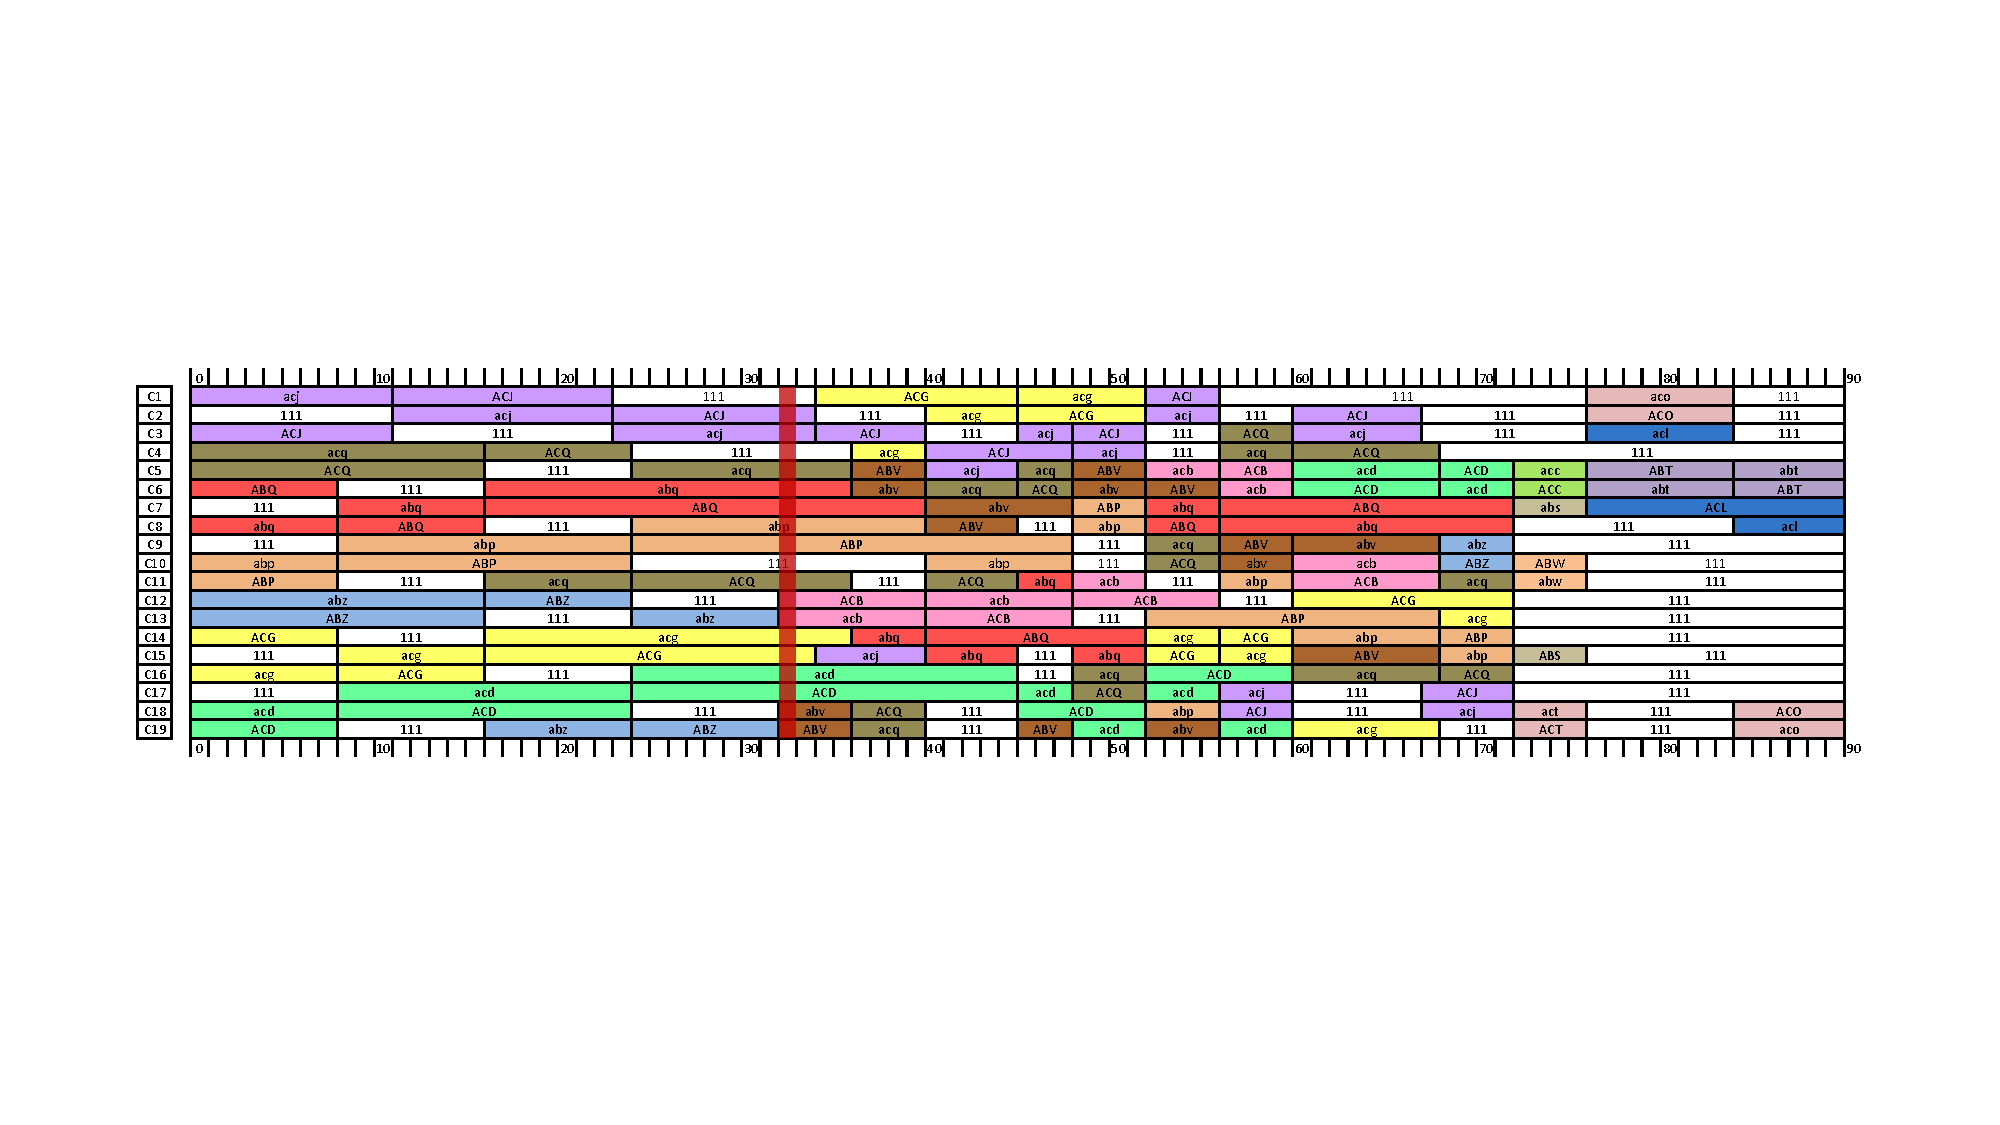
\includegraphics[width=\linewidth]{caso6/caso6-fase2-vns}
	\caption{Solución final (\fasedos{}) para el Caso 6 empleando VNS}
	\label{fig:caso6-fase2-vns}
\end{figure}

\begin{figure}[!]
	\centering
	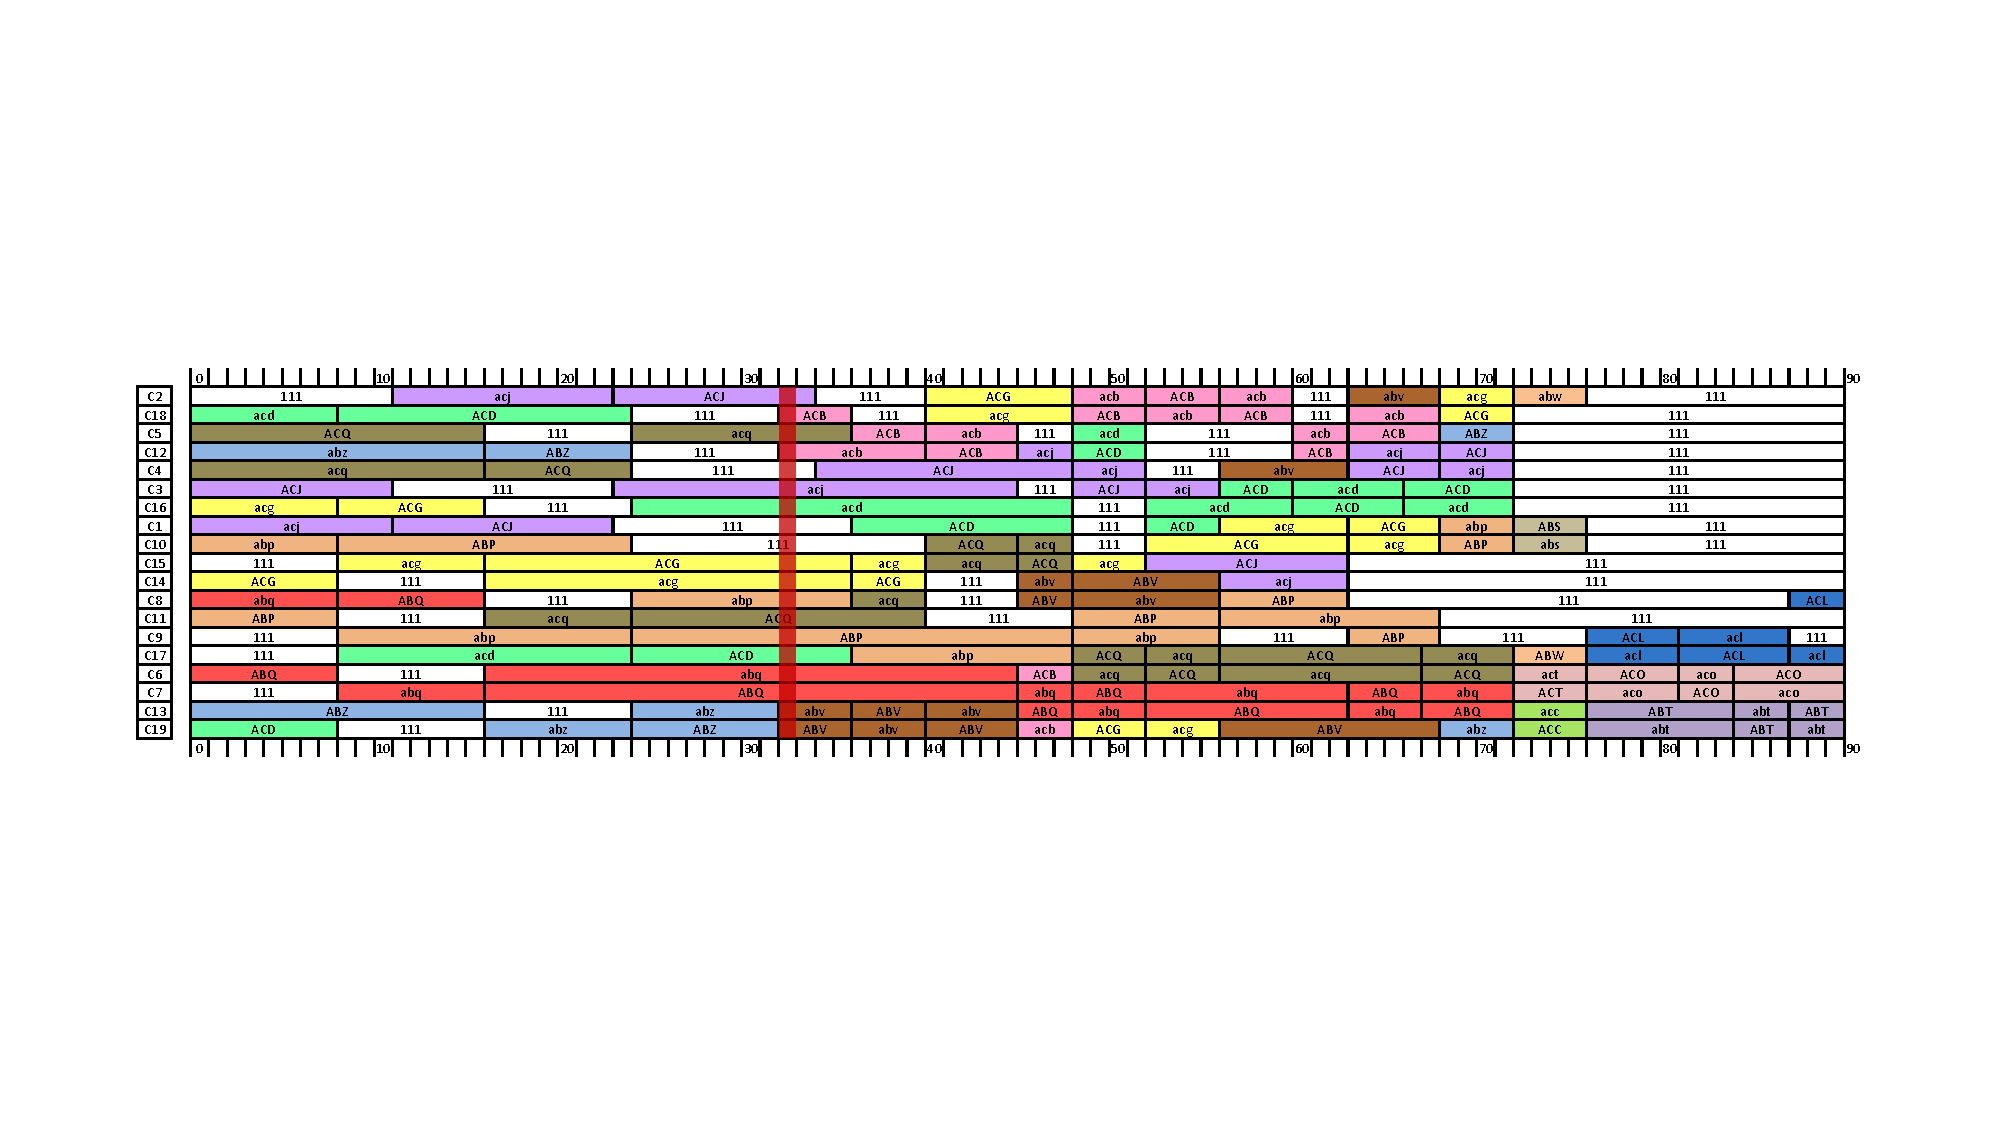
\includegraphics[width=\linewidth]{caso6/caso6-fase2-sa}
	\caption{Solución final (\fasedos{}) para el Caso 6 empleando SA}
	\label{fig:caso6-fase2-sa}
\end{figure}

\subsubsection{Análisis del Caso 8}

El Caso 8 es de los más sencillos, pues únicamente debe gestionar la baja del controlador C16. La planificación inicial es la de la \autoref{fig:caso8-fase0} que se amplía con un controlador imaginario siguiendo la heurística implementada (descrita en la \autoref{sec:baja-alta-controladores}) para la \faseuno{} como muestra la \autoref{fig:caso8-fase1}. 

\begin{figure}[!]
	\centering
	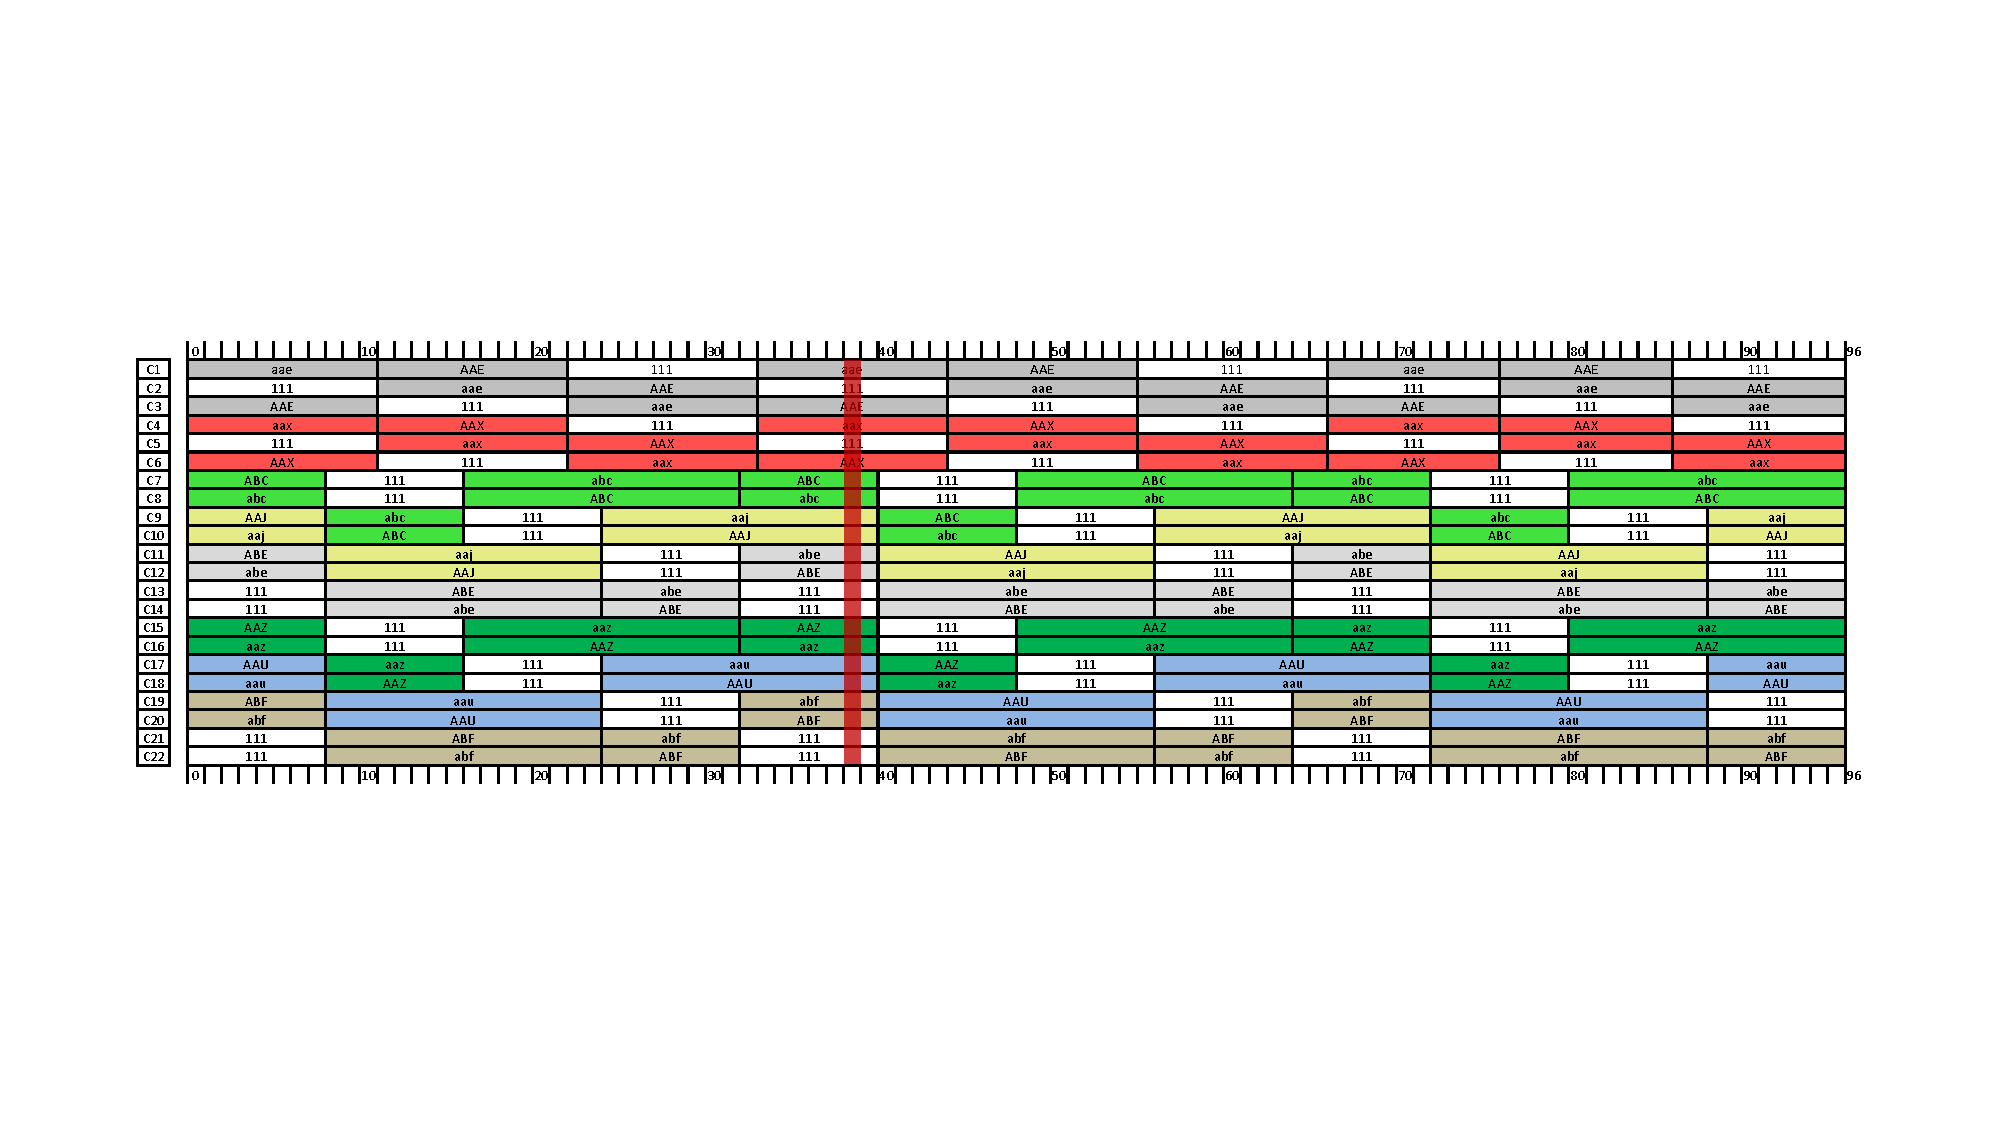
\includegraphics[width=\linewidth]{caso8/caso8-fase0}
	\caption{Planificación inicial para el Caso 8}
	\label{fig:caso8-fase0}
\end{figure}

\begin{figure}[!]
	\centering
	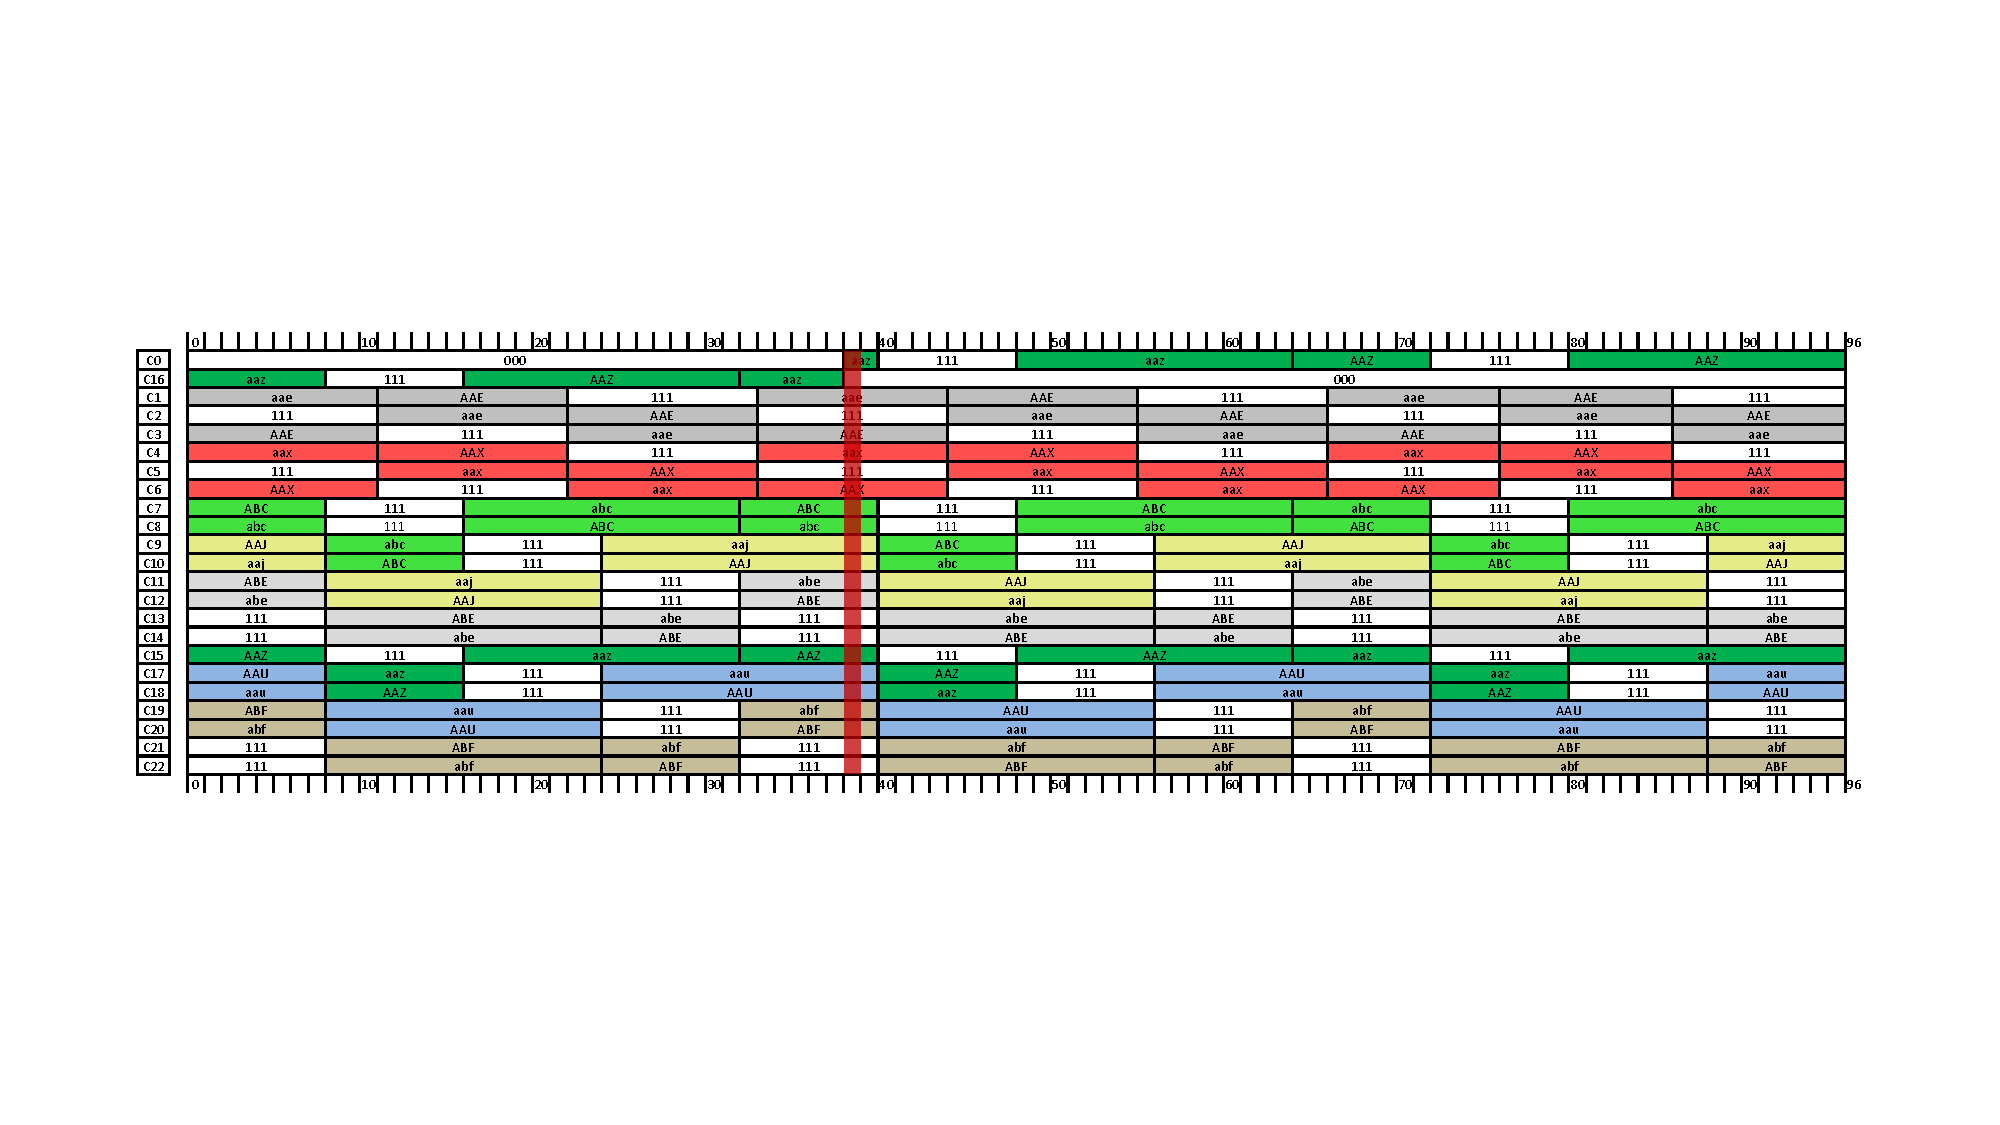
\includegraphics[width=\linewidth]{caso8/caso8-fase1}
	\caption{Solución inicial (\faseuno{}) para el Caso 8}
	\label{fig:caso8-fase1}
\end{figure}

En cuanto al desempeño de la \fasedos{}, ambas opciones agrupan bastante bien los slots como pretende el \ref{O4}. Sin embargo, el VNS logra un mejor resultado en dicho objetivo. El primer objetivo \ref{O1} se logra en ambos casos, eliminando el controlador imaginario añadido en la Fase 1. Aunque para el objetivo de las restricciones, \ref{O2}, en esta solución el SA solo incumple la restricción \ref{RD:12:rotaciones} en 2 ocasiones, mientras que el VNS incumple dos: la restricción \ref{R:5:max-trabajo-continuado} en tres ocasiones y la \ref{RD:3:porcentaje-min-descanso} en dos.
En media, como recogía la \autoref{table:comparativa-sa-vns-porcentaje}, esa mejora de restricciones no es muy significativa.


\begin{figure}[!]
	\centering
	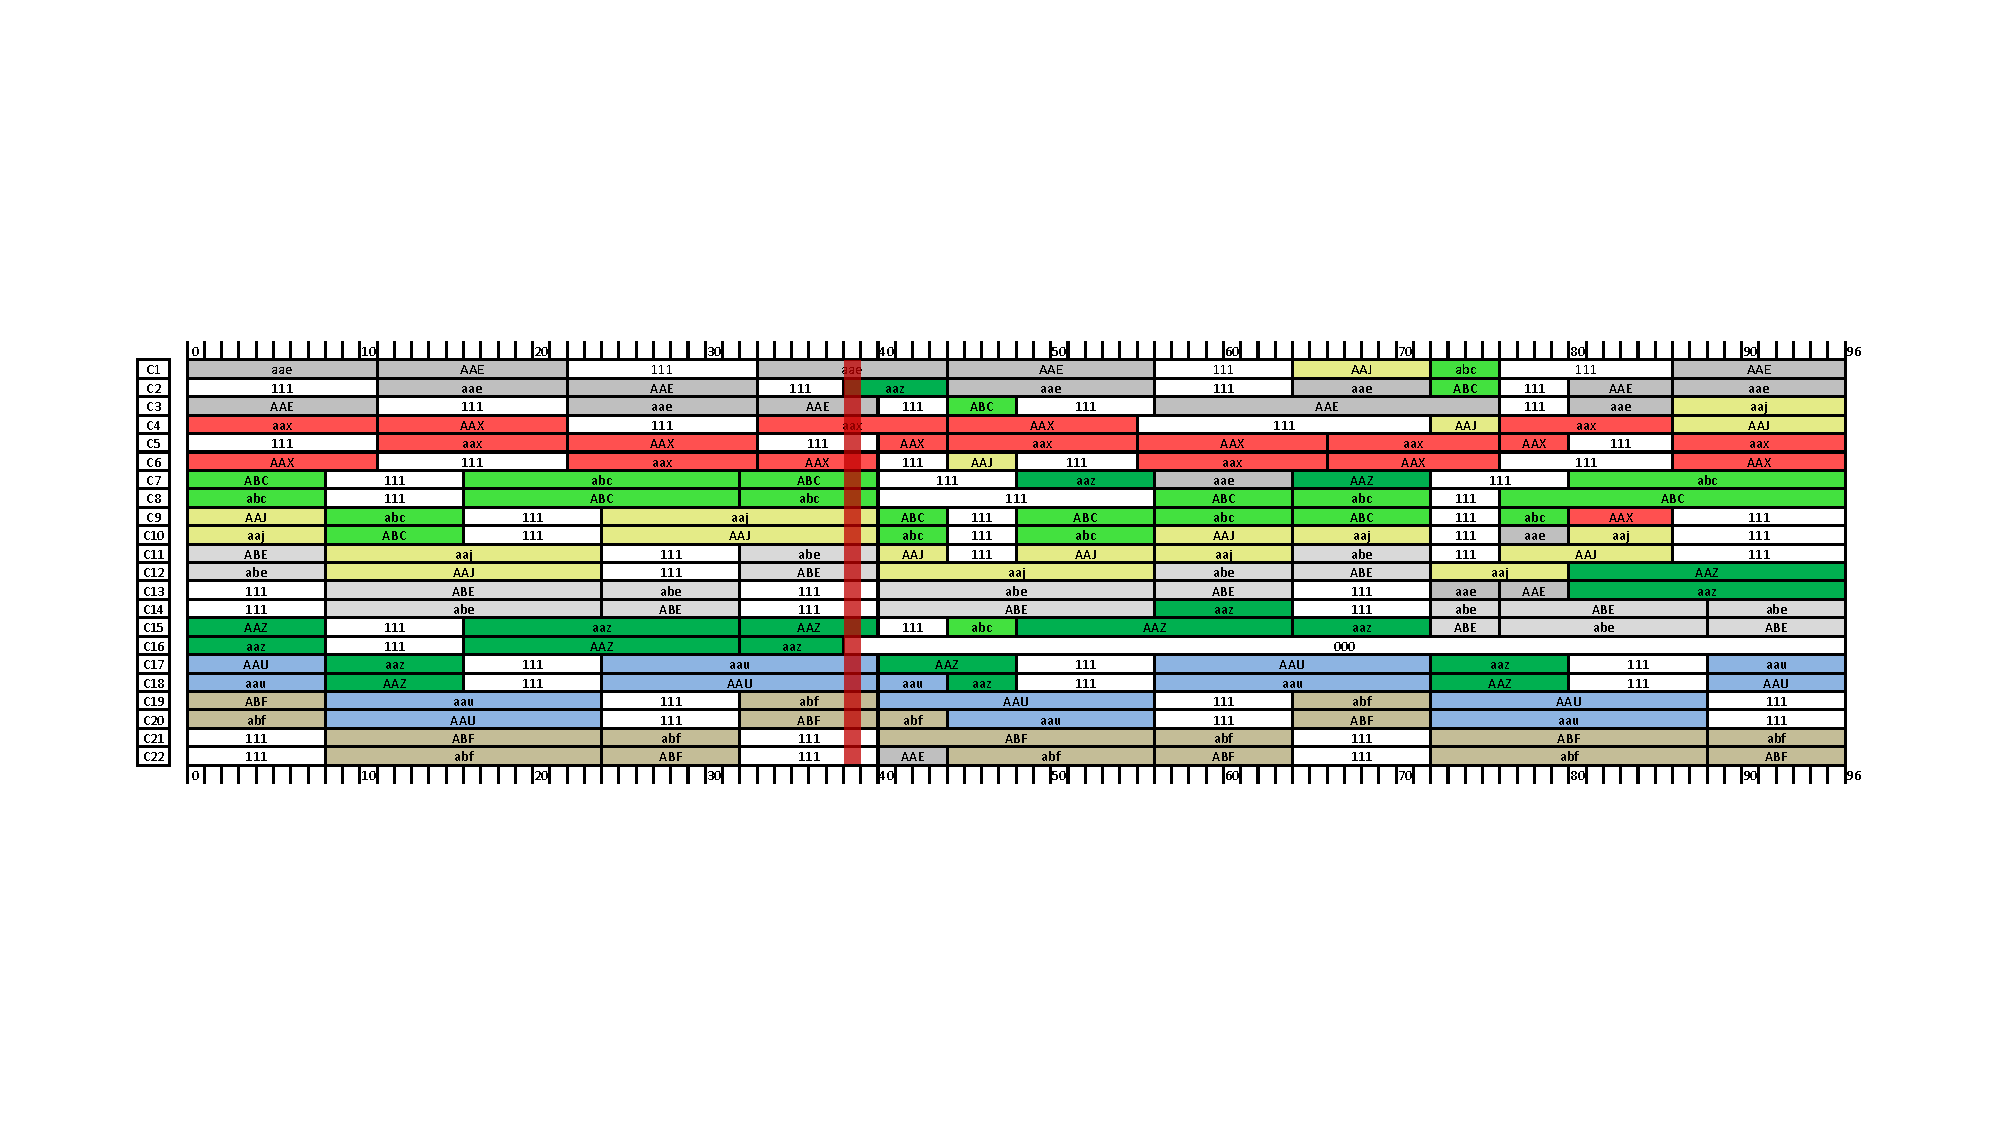
\includegraphics[width=\linewidth]{caso8/caso8-fase2-vns}
	\caption{Solución final (\fasedos{}) para el Caso 8 empleando VNS}
	\label{fig:caso8-fase2-vns}
\end{figure}

\begin{figure}[!]
	\centering
	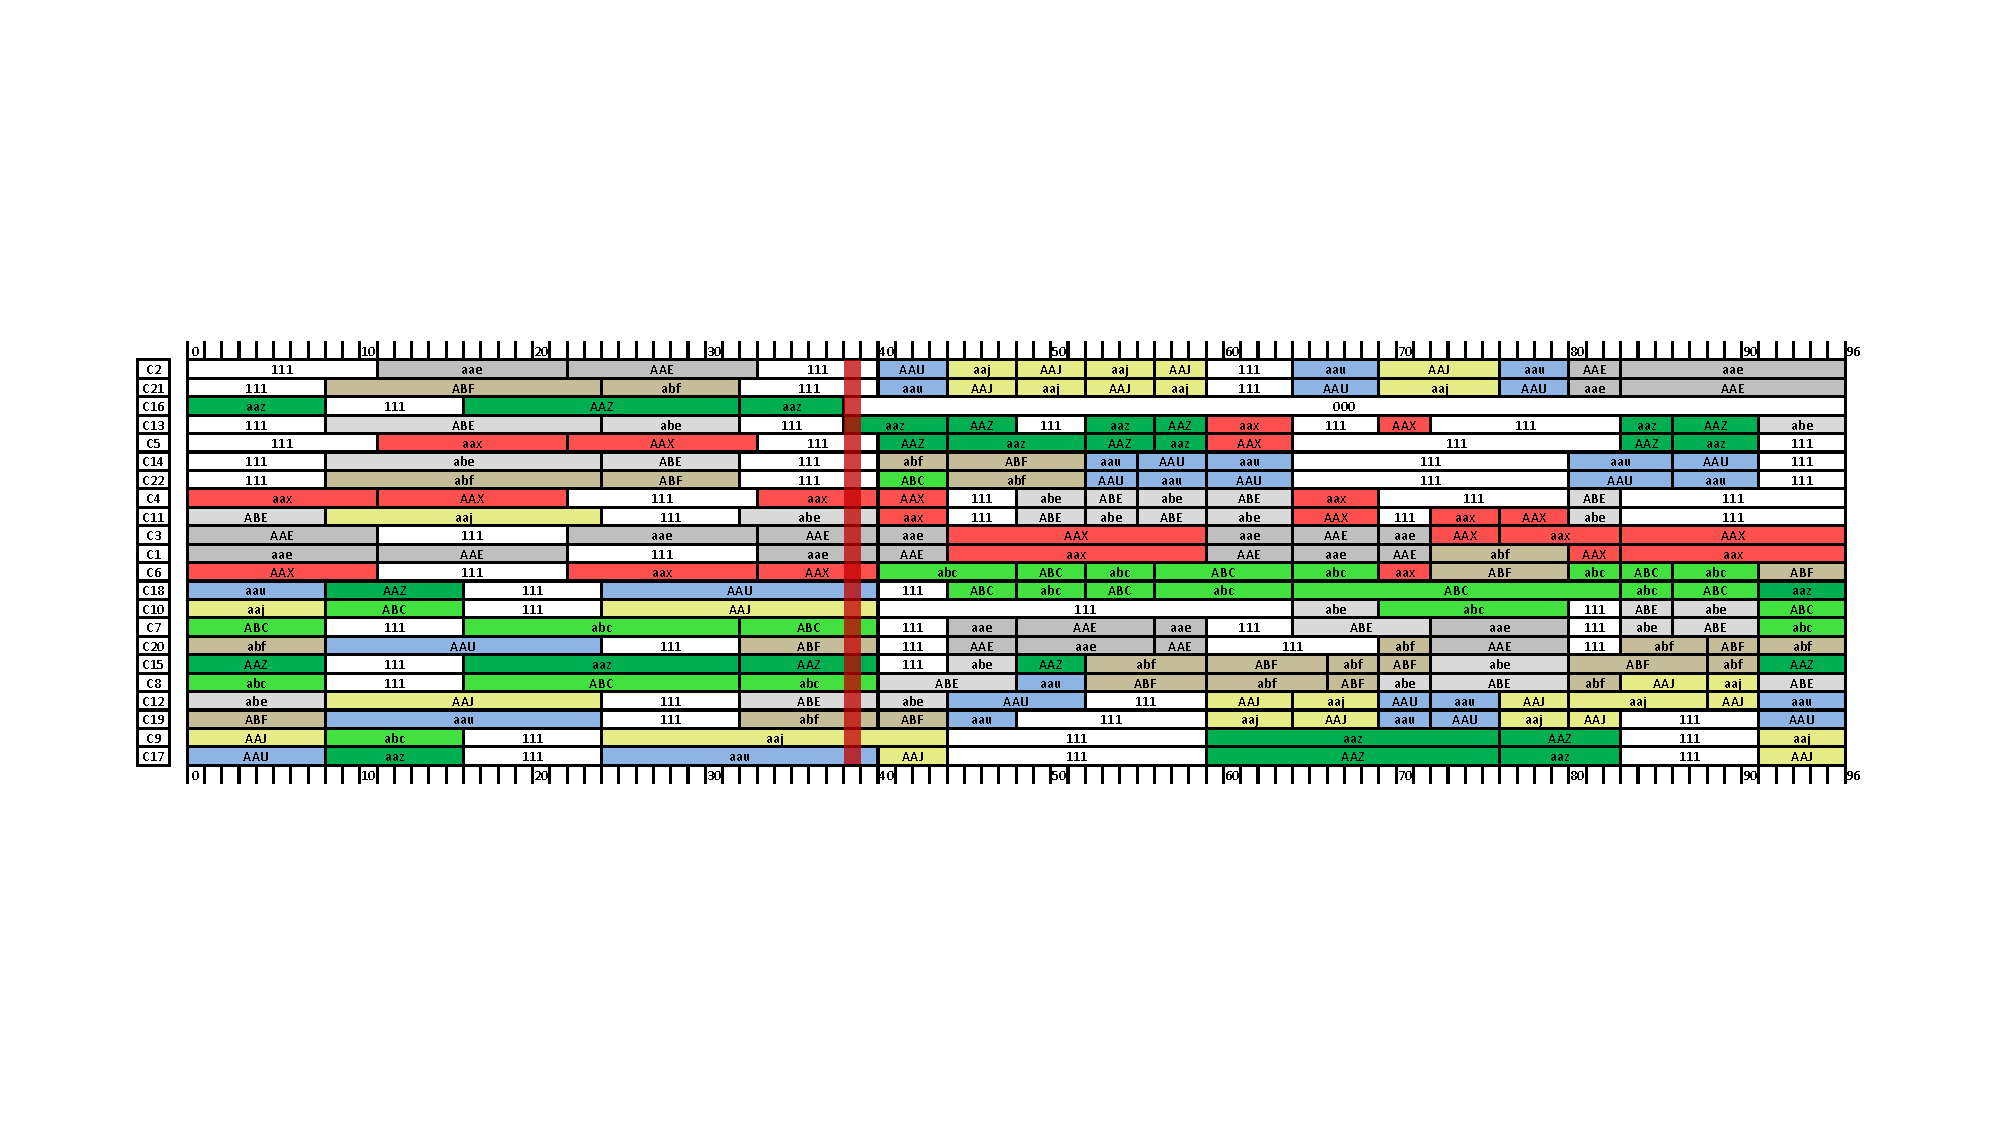
\includegraphics[width=\linewidth]{caso8/caso8-fase2-sa}
	\caption{Solución final (\fasedos{}) para el Caso 8 empleando SA}
	\label{fig:caso8-fase2-sa}
\end{figure}


\subsubsection{Análisis del Caso 9}

El Caso 9 es equivalente al anterior, el Caso 8, con la diferencia de que ahora sí sucede un alta de otro controlador, C23. La planificación inicial es idéntica a la del caso anterior (\autoref{fig:caso8-fase0}) y la solución inicial (tras la \faseuno{}) es la misma pero añadiendo el alta, como muestra la \autoref{fig:caso9-fase1}.

\begin{figure}[!]
	\centering
	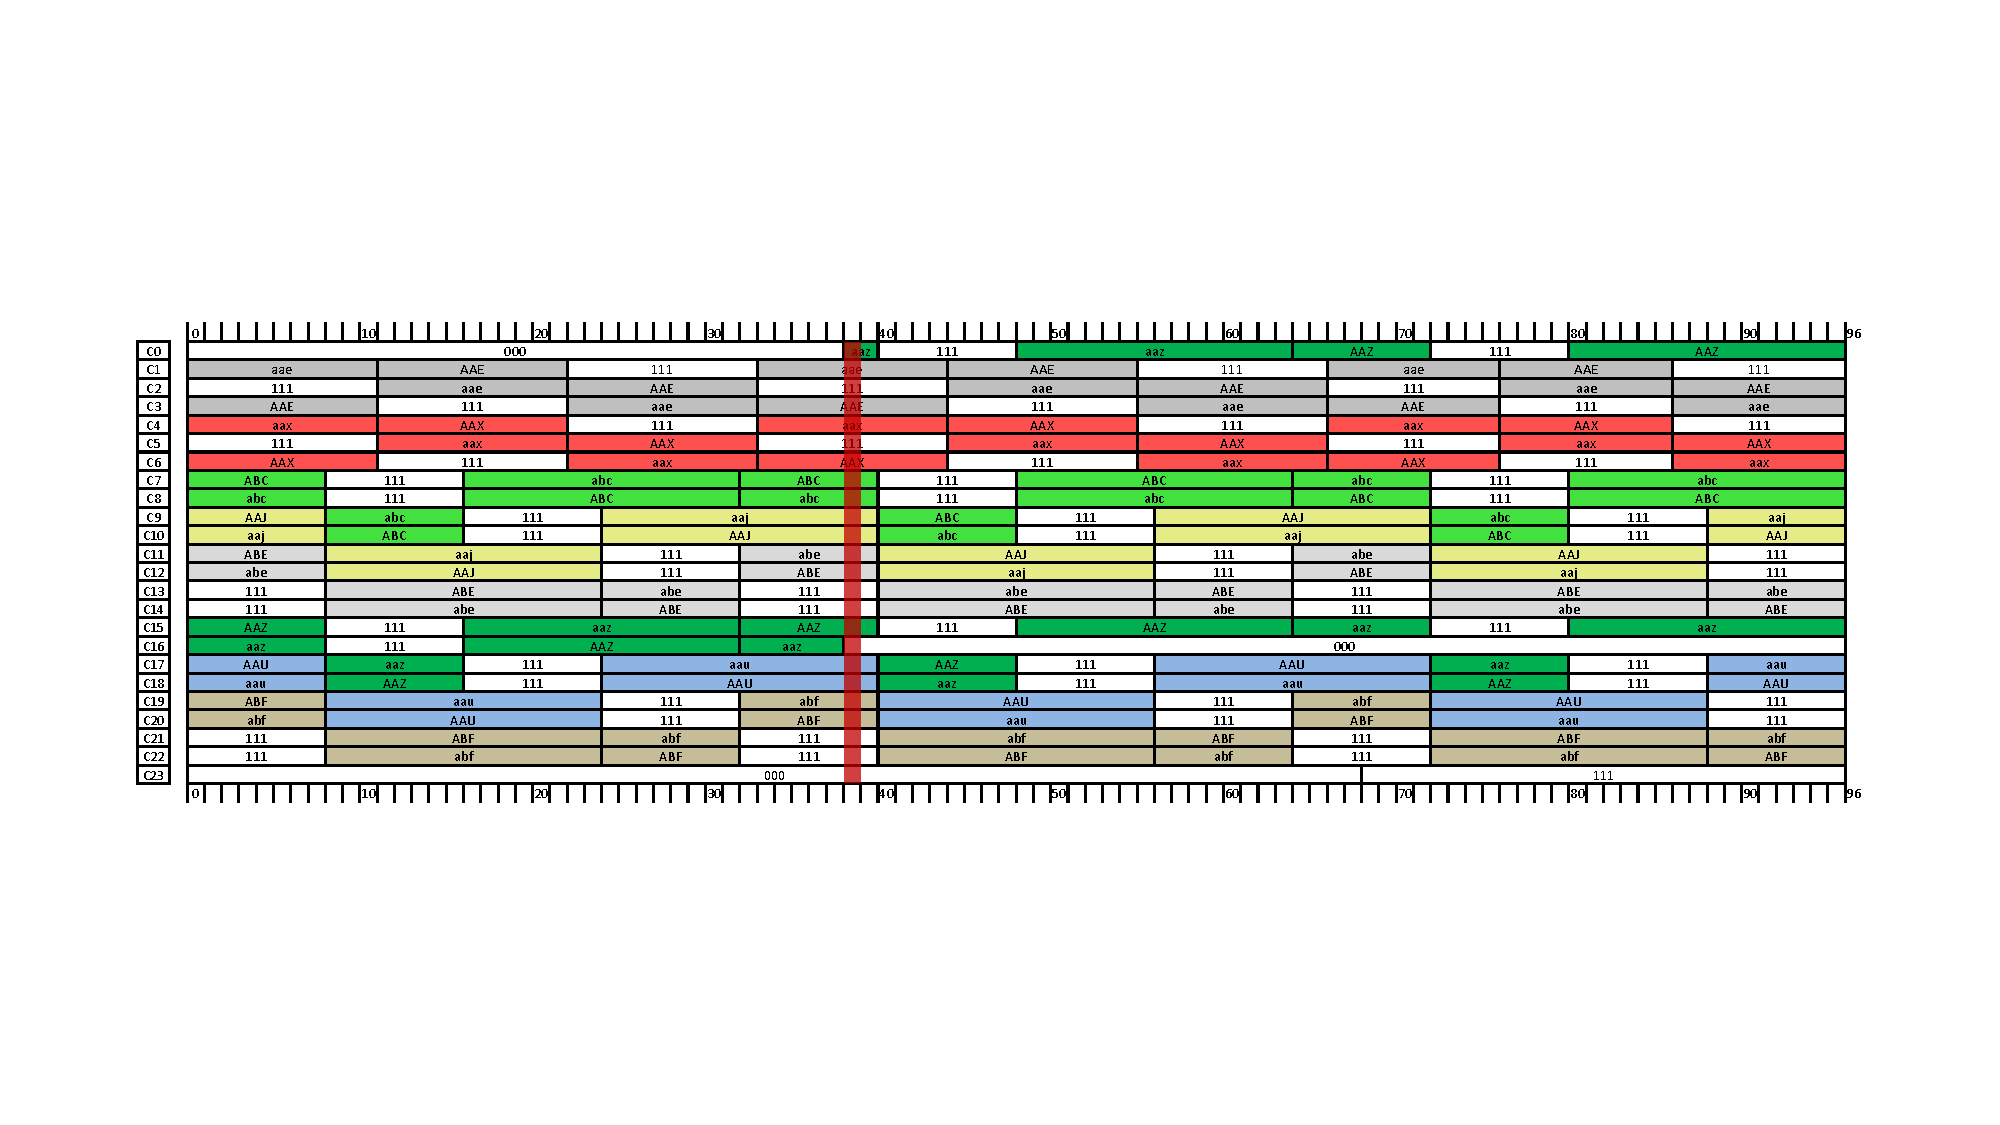
\includegraphics[width=\linewidth]{caso9/caso9-fase1}
	\caption{Solución inicial (\faseuno{}) para el Caso 9}
	\label{fig:caso9-fase1}
\end{figure}

Respecto a la comparación entre metaheurísticas, este es el único caso en el que el SA (\autoref{fig:caso9-fase2-sa}) realmente logra mejores resultados que el VNS (\autoref{fig:caso9-fase2-vns}) con una diferencia significativa. Ambas metaheurísticas logran alcanza el valor máximo del \ref{O1}, sin embargo es en el \ref{O2}, las restricciones incumplidas, aquel objetivo que el SA obtiene valores mayores (es decir, que incumple menos restricciones).

\begin{figure}[!]
	\centering
	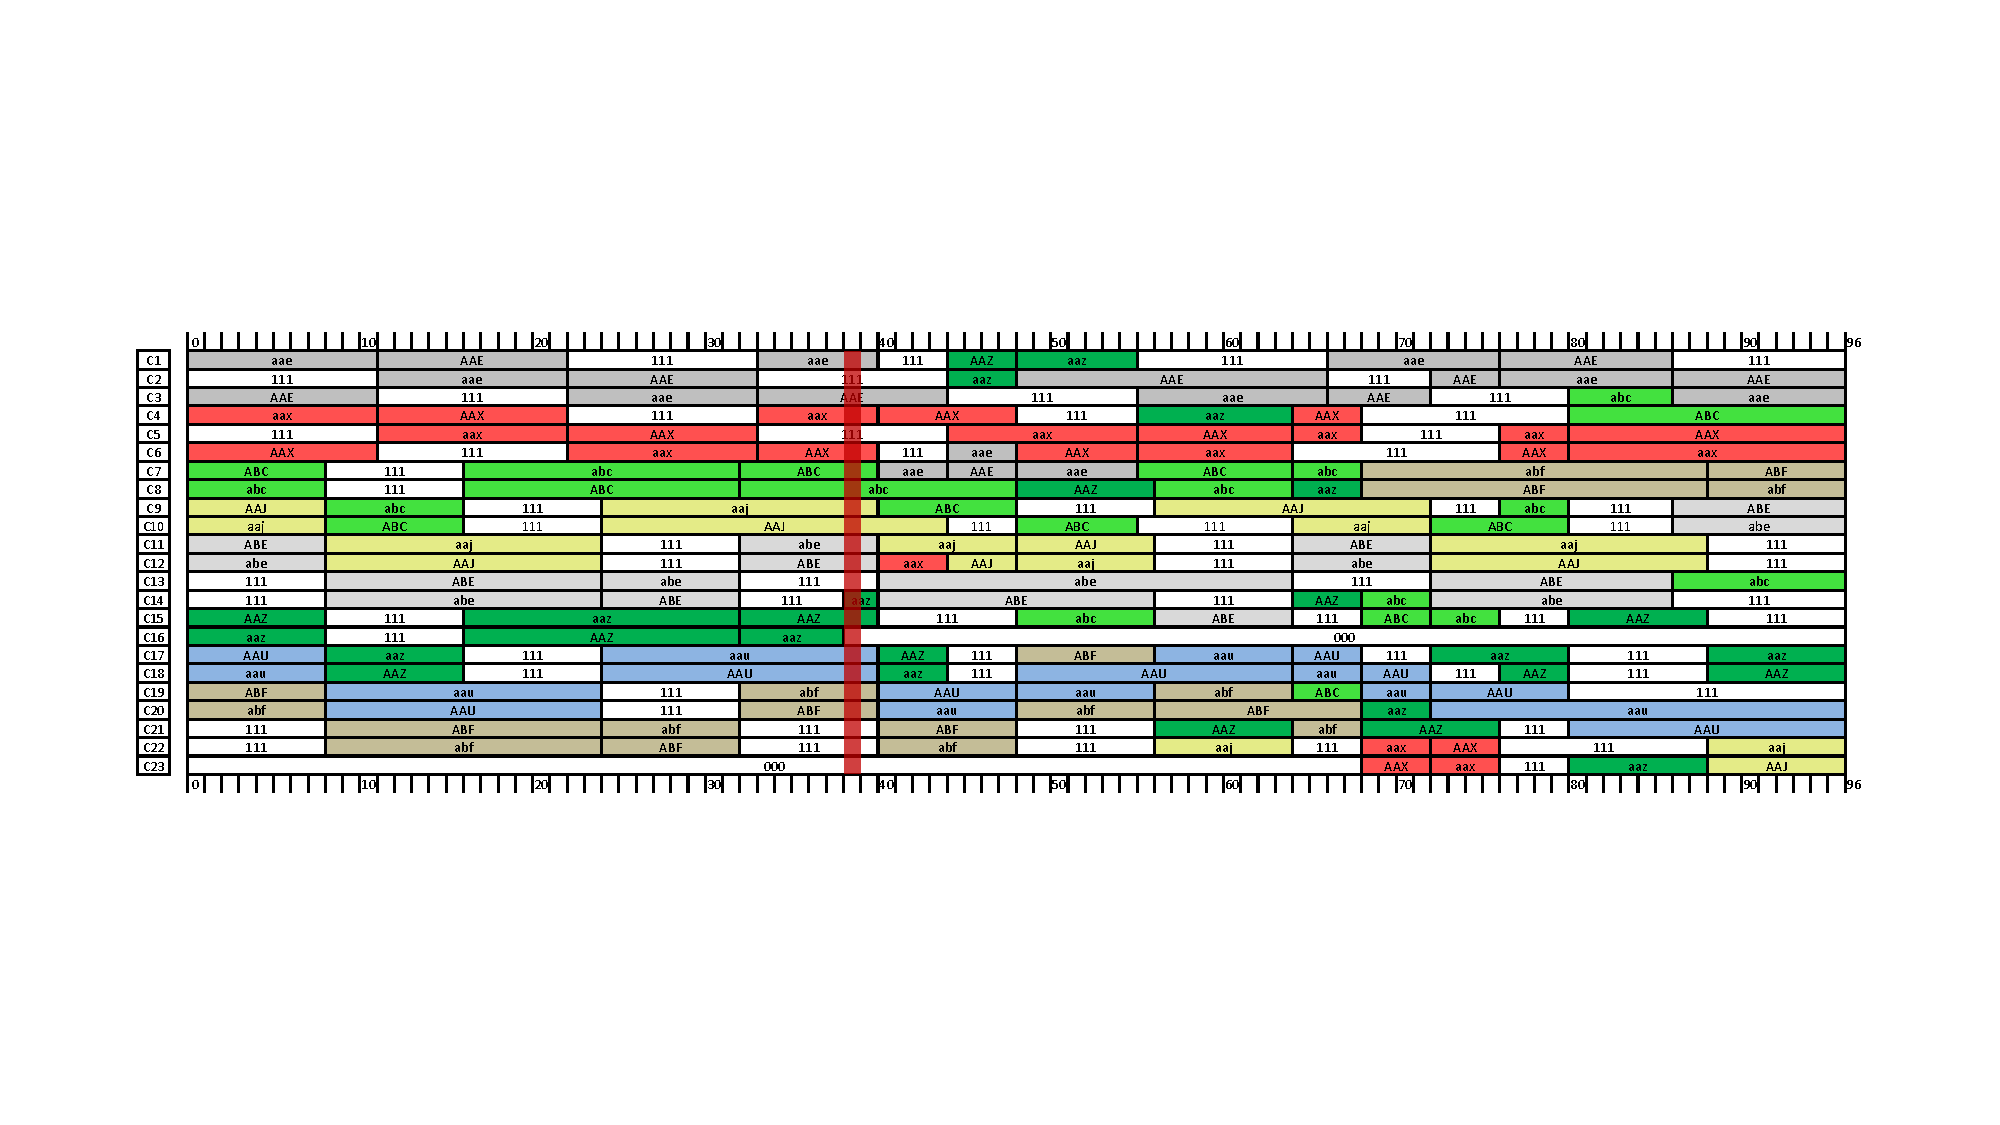
\includegraphics[width=\linewidth]{caso9/caso9-fase2-vns}
	\caption{Solución final (\fasedos{}) para el Caso 9 empleando VNS}
	\label{fig:caso9-fase2-vns}
\end{figure}

\begin{figure}[!]
	\centering
	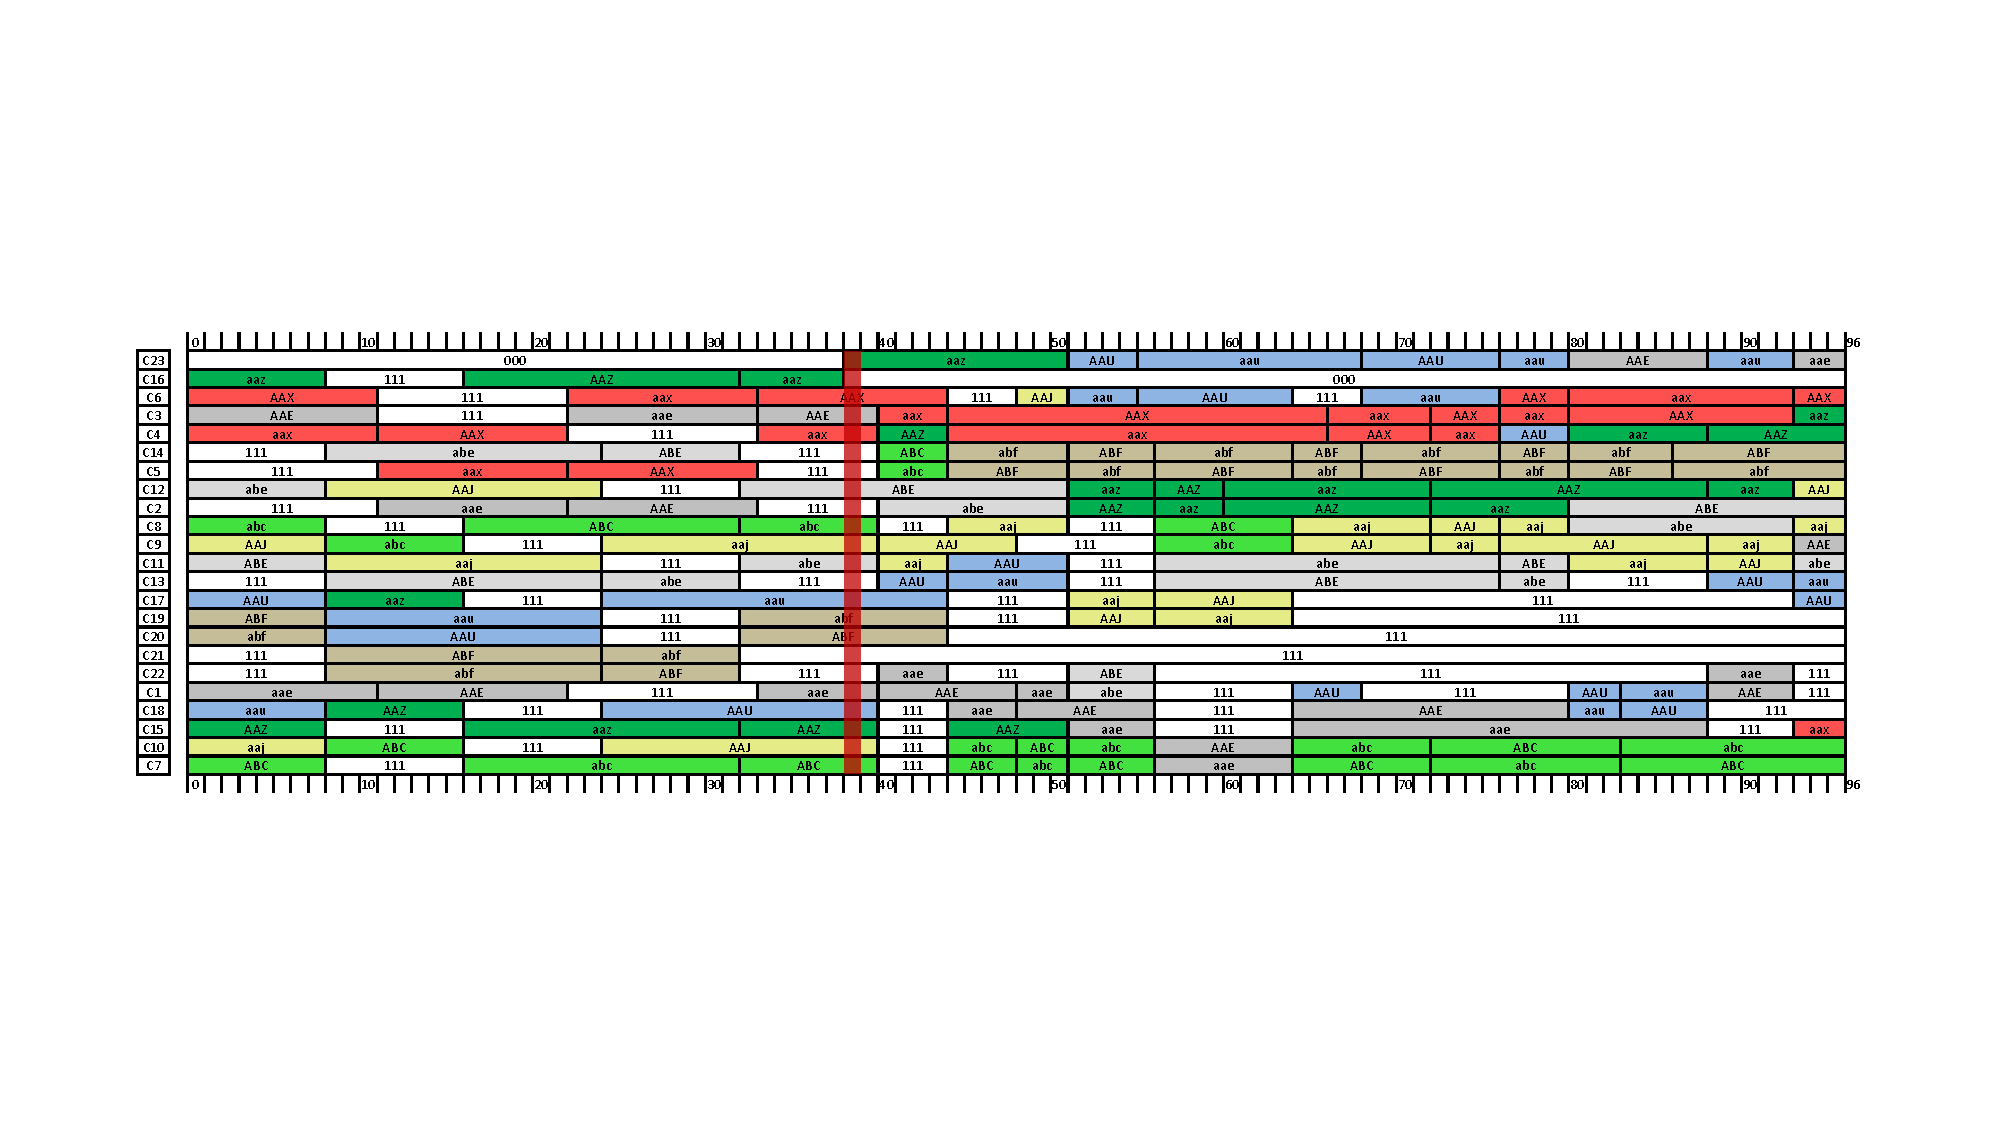
\includegraphics[width=\linewidth]{caso9/caso9-fase2-sa}
	\caption{Solución final (\fasedos{}) para el Caso 9 empleando SA}
	\label{fig:caso9-fase2-sa}
\end{figure}

En las soluciones concretas mostradas anteriormente, el VNS incumple tres veces \ref{RD:3:porcentaje-min-descanso}, cuatro \ref{R:5:max-trabajo-continuado} y una \ref{RD:11:tiempo-min-posicion}; mientras que el SA no incumple ni una sola.

\subsection{Otros experimentos}

En el \autoref{capitulo:3} describimos las alternativas de metodología y parámetros barajadas en el TFM y el porqué fueron elegidas finalmente las empleadas. Una de esas alternativas se trata del comportamiento de la búsqueda local, pudiendo ser \textit{First Improvement} y \textit{Best Improvement}. La segunda, no puede ser aplicada en este problema debido a que no podemos generar todas las posibles soluciones (para quedarnos con la mejor), por lo que se propuso una opción híbrida que precisaba de dos nuevos parámetros al sistema: el número máximo de iteraciones sin mejora para la búsqueda local y el porcentaje mínimo de mejoría para la búsqueda local.

Un experimento interesante puede ser una comparativa entre ambos comportamientos, que puede verse la \autoref{fig:5:first-vs-bestiteracioncaso1}, que representa gráficamente el desempeño medio en cada iteración para el Caso 1, que emplea un \textit{VND}, que es únicamente determinista, por lo que tan solo emplea la búsqueda local como medio de búsqueda dentro del entorno. Se ha llamado al comportamiento híbrido como simplemente \textit{Best Improvement} por ser una adaptación de este.

\begin{figure}
	\centering
	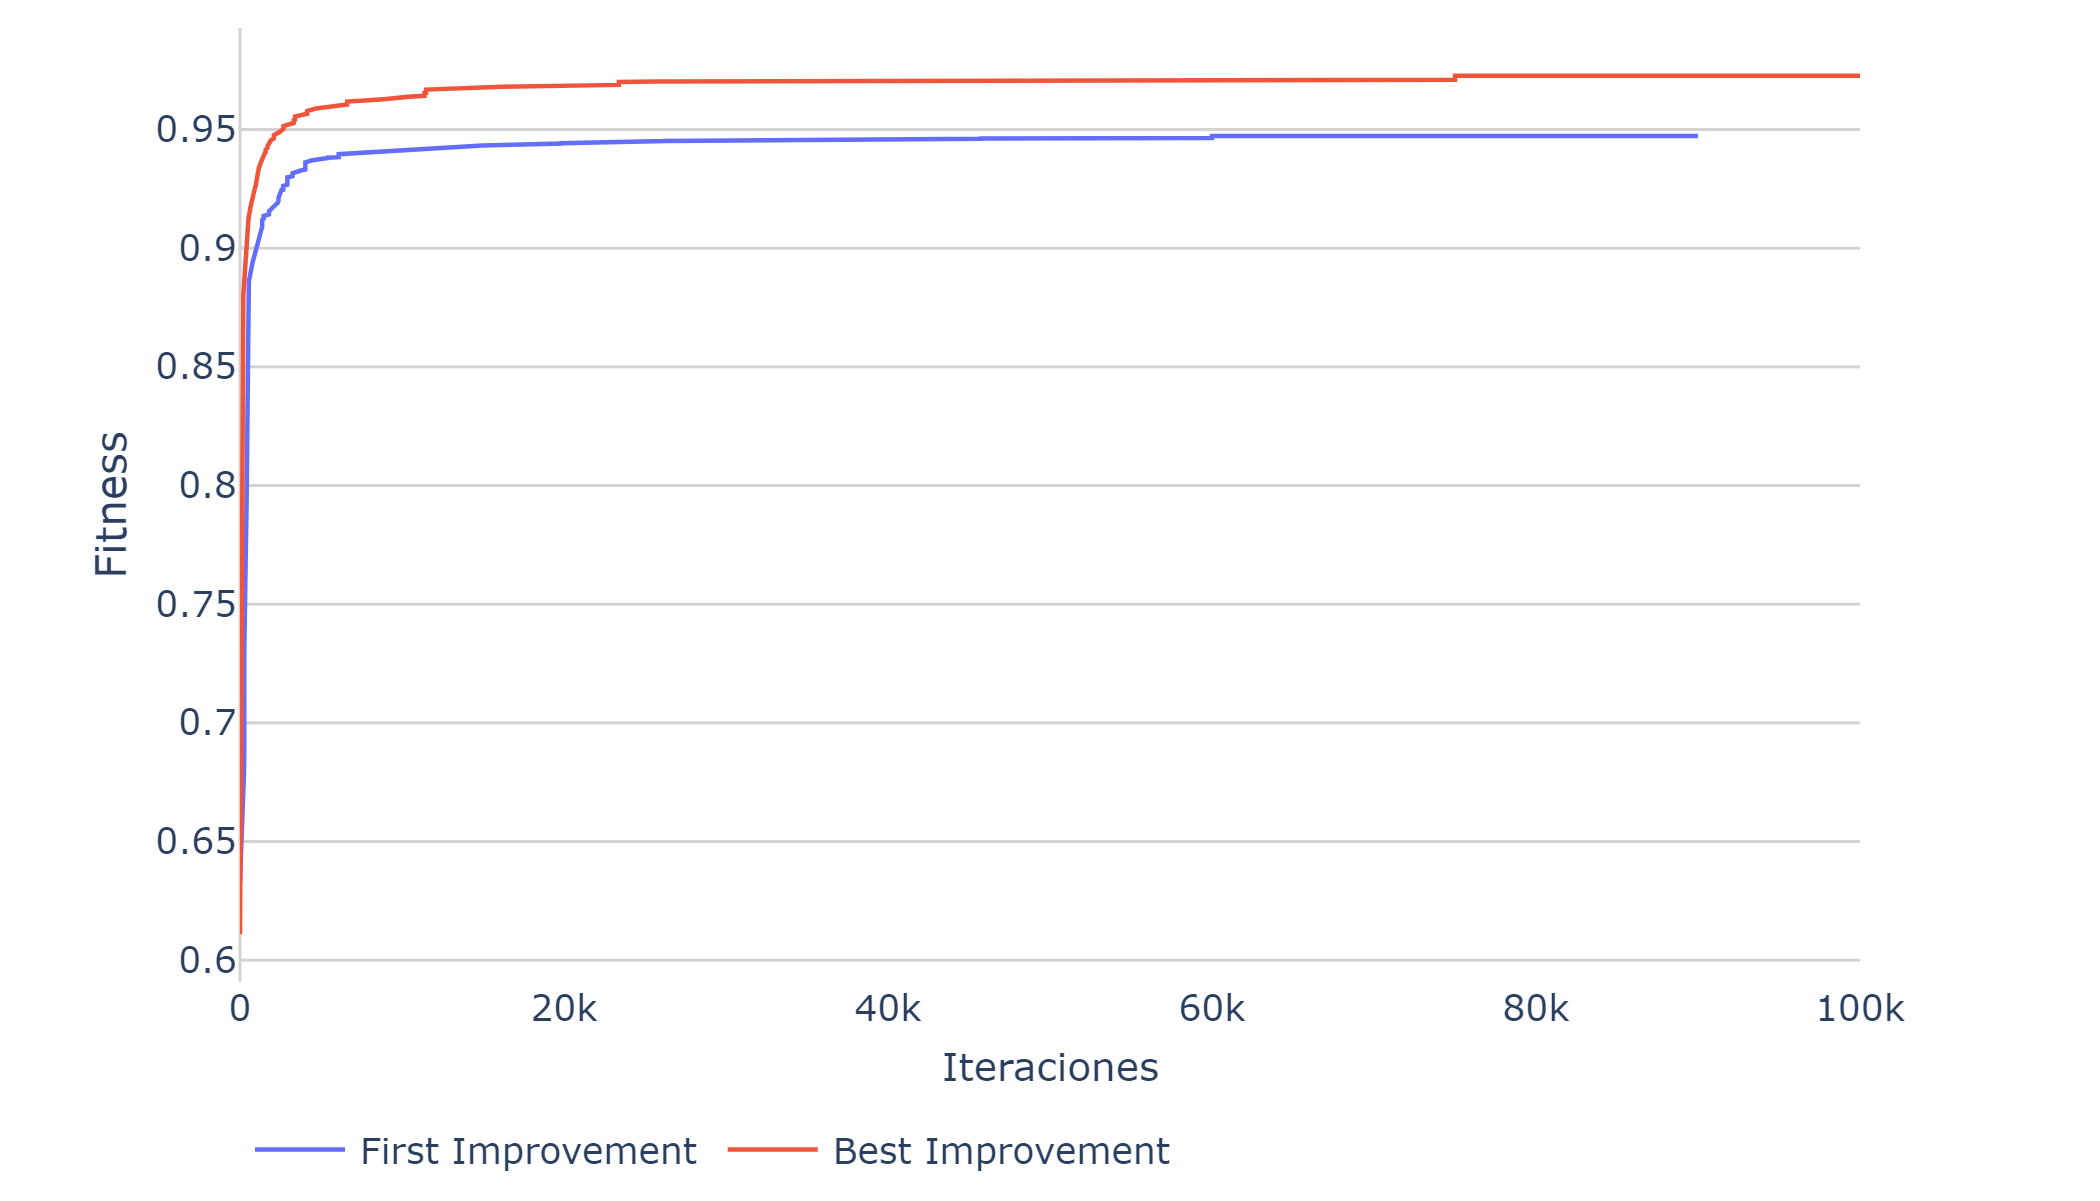
\includegraphics[width=\linewidth]{First-vs-best_iteracion_Caso1}
	\caption{Gráfica comparativa del desempeño del sistema para el Caso 1, empleando los dos posibles comportamientos de la búsqueda local.}
	\label{fig:5:first-vs-bestiteracioncaso1}
\end{figure}

Podemos observar cómo el comportamiento propuesto mejora sustancialmente el desempeño final del algoritmo.